\documentclass[a4paper, 12pt] {report}
\usepackage{graphicx}
\usepackage{amsmath}
\usepackage{wrapfig}
\usepackage{multirow}
\usepackage{float}
\usepackage{csvsimple}
\usepackage{makecell}
\usepackage{fancyvrb, fancybox, calc}
\usepackage{color}
\usepackage{hyperref}
\usepackage[english]{babel}
\usepackage[svgnames]{xcolor}
\usepackage{apacite}
\hypersetup{
    colorlinks=true,
    linkcolor=black,
    filecolor=magenta,      
    urlcolor=blue,
    citecolor=black}
\urlstyle{same}
\usepackage{lineno}

\renewcommand{\familydefault}{\sfdefault}

\newenvironment{verbcode}{\VerbatimEnvironment% 
  \noindent
  %      {\columnwidth-\leftmargin-\rightmargin-2\fboxsep-2\fboxrule-4pt} 
\color{white}
  \begin{Sbox} 

  \begin{minipage}{\linewidth-2\fboxsep-2\fboxrule-4pt}    
  \begin{Verbatim}[commandchars=\\\{\}]
\textcolor{white}{}
}{% 
  \end{Verbatim}  
  \end{minipage}   
  \end{Sbox} 
  \fcolorbox{black}{black}{\TheSbox} 
} 

\begin{document}


     \title{%
University of Virginia Forest Model Enhanced \\
\large Version 3 - July 2022\\
---\\
\large Technical Documentation 
}
\author{Adrianna Foster}
     \maketitle

\tableofcontents

\chapter{Introduction} \label{chap:intro}
\section{Model Structure}
The University of Virginia Forest Model Enhanced (UVAFME) is an update and extension of the individual-based gap model FAREAST \cite{yanFAREASTForestGap2005}. As a traditional gap model, UVAFME simulates the establishment, growth, and mortality of individual trees and shrubs (as of version 3) on independent patches (i.e. plots) of a forested landscape (Fig. \ref{fig:maindiagram}). The model is only spatially distributed in the vertical dimension, and plots are assumed to have no direct spatial interactions with one another. Through a Monte Carlo-style aggregation, the average of several hundred of these independent patches represents the average expected conditions of a forested landscape through time. As such, output from UVAFME is comparable to a statistically robust sampling of replicate forest inventory plots \cite{shugartGlobalChangeTerrestrial2011, shugartGapModelsTheir2018}.

\begin{figure}
  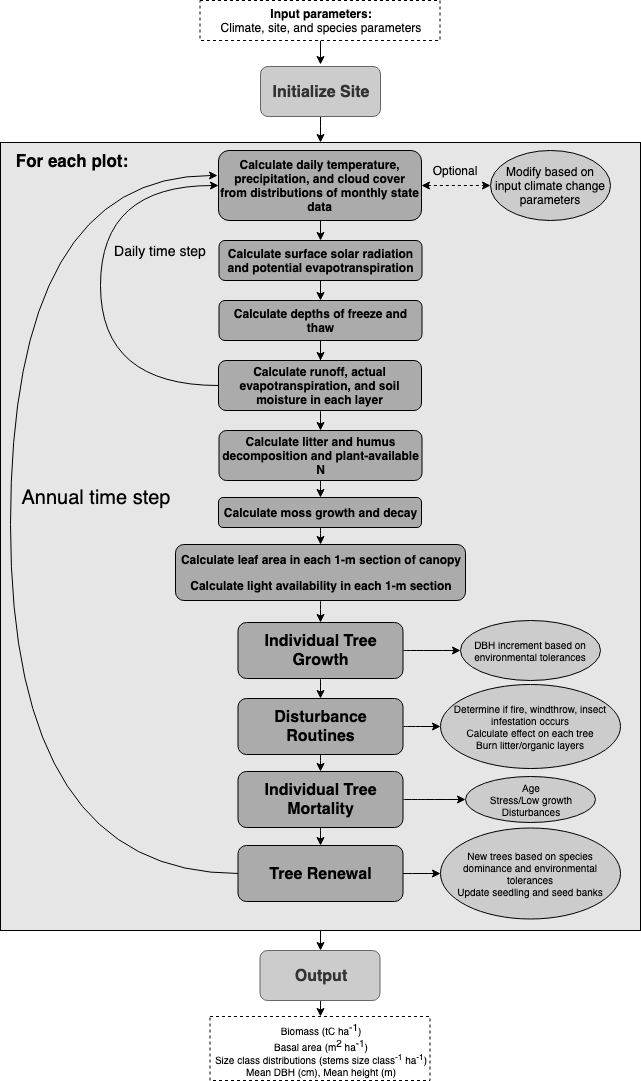
\includegraphics[width=\linewidth]{Figures/UVAFME_MainSchematic.png}
  \caption{Main structure of UVAFME.}
  \label{fig:maindiagram}
\end{figure}

Climate is based on input distributions of monthly precipitation, temperature, cloud cover, and relative humidity, derived from the historical data record. Daily soil moisture and nutrient dynamics are simulated based on a coupled, two-layer soil submodule using input site and soil characteristics.

Individual plant growth for each year is calculated through optimal diameter increment growth, modified by available resources and species- and plant size-specific tolerances to temperature and permafrost (if present), and light, moisture, and nutrient availability. Individual plants can thus compete with one another for above- and belowground resources. Light availability throughout the canopy is calculated using the Beer-Lambert Law and is dependent on the vertical distribution of leaf area within the plot. Tree/shrub growth response to temperature is based on an asymptotic relationship between growth rate and annual growing degree-days. Drought response is based on an index that represents the proportion of the growing season that experiences soil moisture limitation and/or high atmospheric demand. Nutrient availability response is based on responses to a relative nitrogen availability variable, calculated by comparing plant-available N (simulated in the decomposition subroutine) to the required N that year. The final annual increment growth for each plant is determined by multiplying the smallest (i.e. most limiting) growth-limiting factor by the optimal increment growth. Establishment of seedlings and saplings is based on species-specific resources and environmental tolerances as well as plot conditions. 

Trees and shrubs may die from age- or growth stress-related factors or by disturbances (i.e. fire, windthrow, or insect infestation). Fire and windthrow occurrence are probabilistic, based on site-specific mean return intervals. Fire and windthrow mortality are based on intensity (for fire), as well as species- and size-specific tolerances. Insect infestation is based on plant- and stand-level factors that increase probability of infestation and mortality. Plants that die, as well as annual leaf litter and woody debris are transferred to litter cohorts for decomposition.

\subsection{Scale and Spatial Interaction} \label{scales}

Currently, UVAFME sites do not interact with one another and thus may be run in parallel or in sequence. Within a site, several hundred (generally 200) independent plots about the area of influence of a dominant tree crown (e.g. 500 m$^{2}$) are simulated that represent patches of a forested landscape (Fig. \ref{fig:scales}b). Forest ``landscape" in this context is defined as a dynamic mosaic of forest gaps (i.e. patches/plots) \cite{shugartModelingForestLandscapes1985}. Within each patch, gap dynamics play out through the establishment of new plants following some major disturbance, growth and competition between plants to fill in the gap,  eventual dominance or co-dominance of a few trees, and death of such canopy dominants, which starts the cycle anew (Fig. \ref{fig:scales}c) \cite{shugartTheoryForestDynamics1984}. Within UVAFME, the plots do not interact with one another, and thus represent independent replicates of potential forest dynamics occurring at a location with input environmental and climatological conditions. Due to the stochastic factors within UVAFME (i.e. disturbances, mortality, and regeneration; see Sections \ref{mortality} and \ref{regen}), each plot represents a forest patch undergoing some gap dynamics process, driven by both deterministic processes (e.g. plant growth response to external factors; Section \ref{gmult}) and stochastic factors (e.g. mortality and disturbance events; Section \ref{mortality}). A Monte Carlo-style average of such plots thus represents average, non-spatially explicit (i.e. per area) \textit{expected} forested conditions for the site location (Fig. \ref{fig:scales}d, e). This aggregation also produces emergent properties at the landscape scale (i.e. the average of several hundred gaps) such as forest succession (Fig. \ref{fig:scales}e), cyclical effects \shortcite{fosterModelbasedEvidenceCyclic2015, emanuelSpectralAnalysisForest1978, pastorSuccessionalChangesNitrogen1987}, and response to shifting climate and disturbance regimes \cite{fosterValidationApplicationForest2017, shumanFireDisturbanceClimate2017, shugartGapModelsTheir2018}.

Climate and daily weather conditions in UVAFME are the same across all plots within a site, thus each plot experiences the same temperature, precipitation, cloud cover, and PET each simulation day. As of Version 3 of UVAFME, soil conditions within each plot are independent of one another, driven by the site-wide factors such as climate and input/initial soil conditions, as well as plot-specific factors such as forest cover and disturbances (Sections \ref{soil} and \ref{disturbances}). Additionally, within each plot individual plants are placed on a 30$\times$30 grid. Each plot is assumed to be horizontally (but not vertically) homogeneous with respect to canopy cover and leaf area, seed rain and seedling banks, as well as soil conditions.

\begin{figure}
  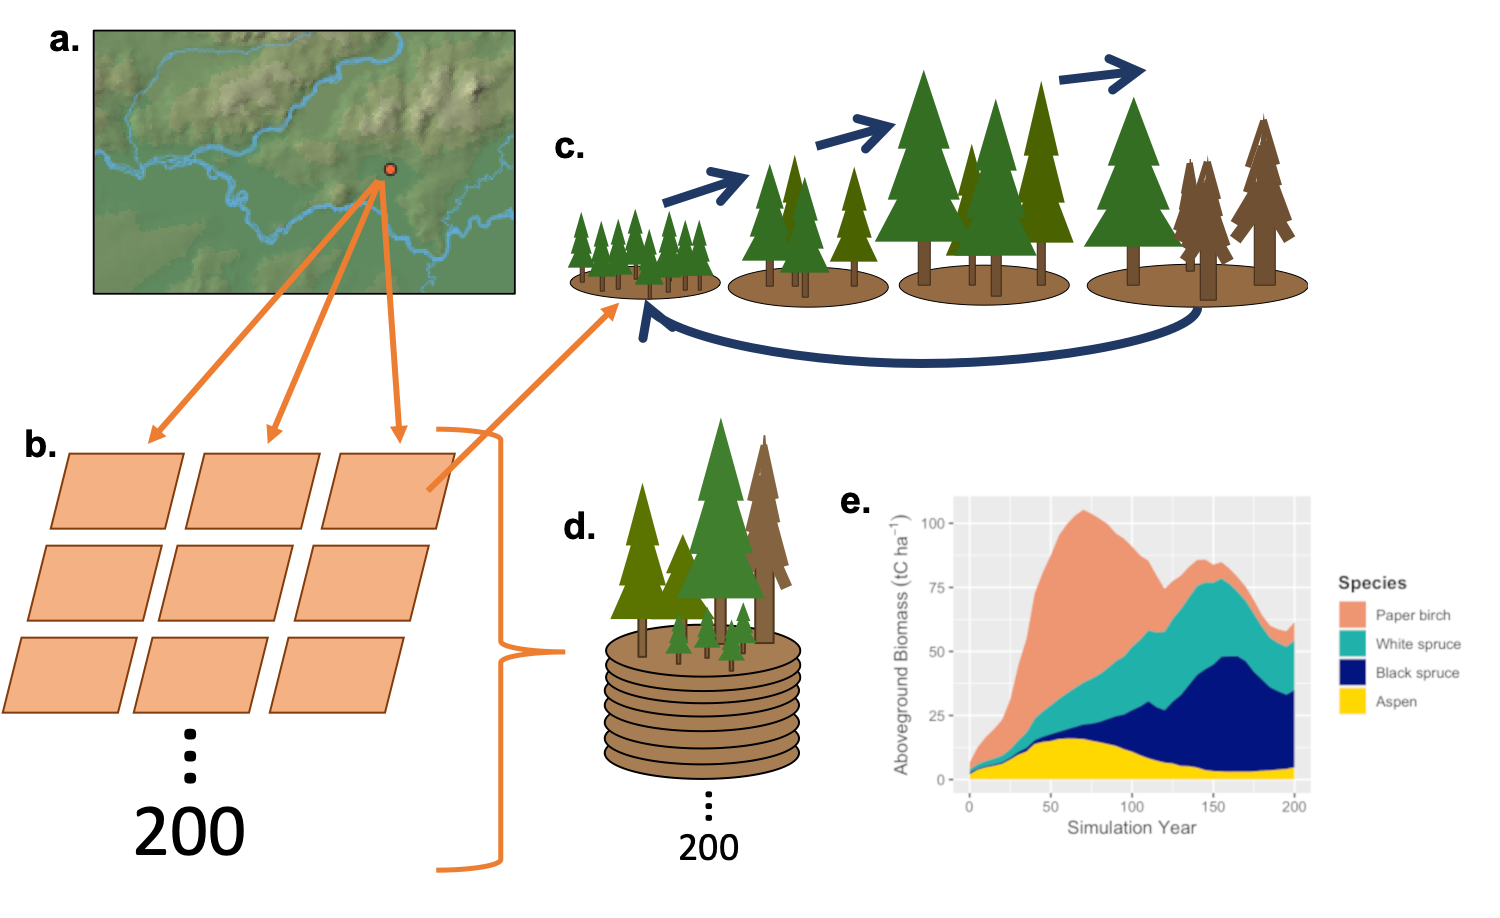
\includegraphics[width=\linewidth]{Figures/Scales_full.png}
  \caption{A single site simulated with UVAFME (a) contains several hundred independent plots (b), each undergoing independent gap dynamics processes (c). These plots are averaged together (d) to produce landscape-scale expected forested conditions over time, from bare-ground initiation and through forest succession (e).}
  \label{fig:scales}
\end{figure}

\chapter{Model Equations and Processes} \label{chap:modelproc}

\section{Climate} \label{climate}

\subsection{Temperature, Precipitation, and Cloud Cover} \label{weather}
\numberwithin{equation}{section}

Climate in UVAFME is simulated through input distributions of monthly temperature (ºC), precipitation (cm), cloud cover (tenths of sky covered), and relative humidity (\%). The average monthly minimum and maximum temperatures, precipitation, cloud cover, and relative humidity, as well as standard deviations for these values (generally derived from at least 30 years of historical climate data) are used to create a range of possible values for a site in question. Monthly and daily weather conditions are the same across all plots within a site.

\subsubsection{Monthly Weather Values}

The input distributions of climate variables are used to generate daily values of maximum temperature ($t_{max}$), minimum temperature ($t_{min}$), precipitation ($p$), cloudiness ($c$), and relative humidity ($RH$), throughout the simulation. For each year, the input mean monthly values are used to generate monthly values for that year using the variable's standard deviation and a normally distributed random number (mean = 0.0, sd = 1.0) between -1.0 and 1.0 for temperature, cloud cover, and humidity, and -0.5 and 0.5 for precipitation (see Section \ref{random} on random processes):

\begin{equation}
t_m = \bar{t}_m + \bar{t}_{sd} t_f
\end{equation}

\begin{equation}
p_m = \max{(\bar{p}_m + \bar{p}_{sd} p_f, 0.0)}
\end{equation}

\begin{equation}
c_m = \max{(\bar{c}_m + \bar{c}_{sd} c_f, 0.0)}
\end{equation}

\begin{equation}
RH_m = \max{(\bar{RH}_m + \bar{RH}_{sd} RH_f, 0.0)}
\end{equation}

where $t_m$ is the monthly minimum or maximum temperature for a particular simulated month, $\bar{t}_m$ and $\bar{t}_{sd}$ are the input average and standard deviations of temperature (minimum or maximum) for that month, $p_m$ is the monthly precipitation for a particular simulated month, $\bar{p}_m$ and $\bar{p}_{sd}$ are the input average and standard deviations of precipitation for that month, $c_m$ is the monthly cloud cover for a particular simulated month, $\bar{c}_m$ and $\bar{c}_{sd}$ are the input average and standard deviations of cloud cover for that month, $RH_m$ is the mean monthly relative humidity for a particular simulated month, $\bar{RH}_m$ and $\bar{RH}_{sd}$ are the input average and standard deviations of relative humidity for that month, and $t_f$, $p_f$, $c_f$, and $RH_f$ are normally distributed random numbers, generated anew for each month of each year (see Section \ref{random}).

\begin{figure}
  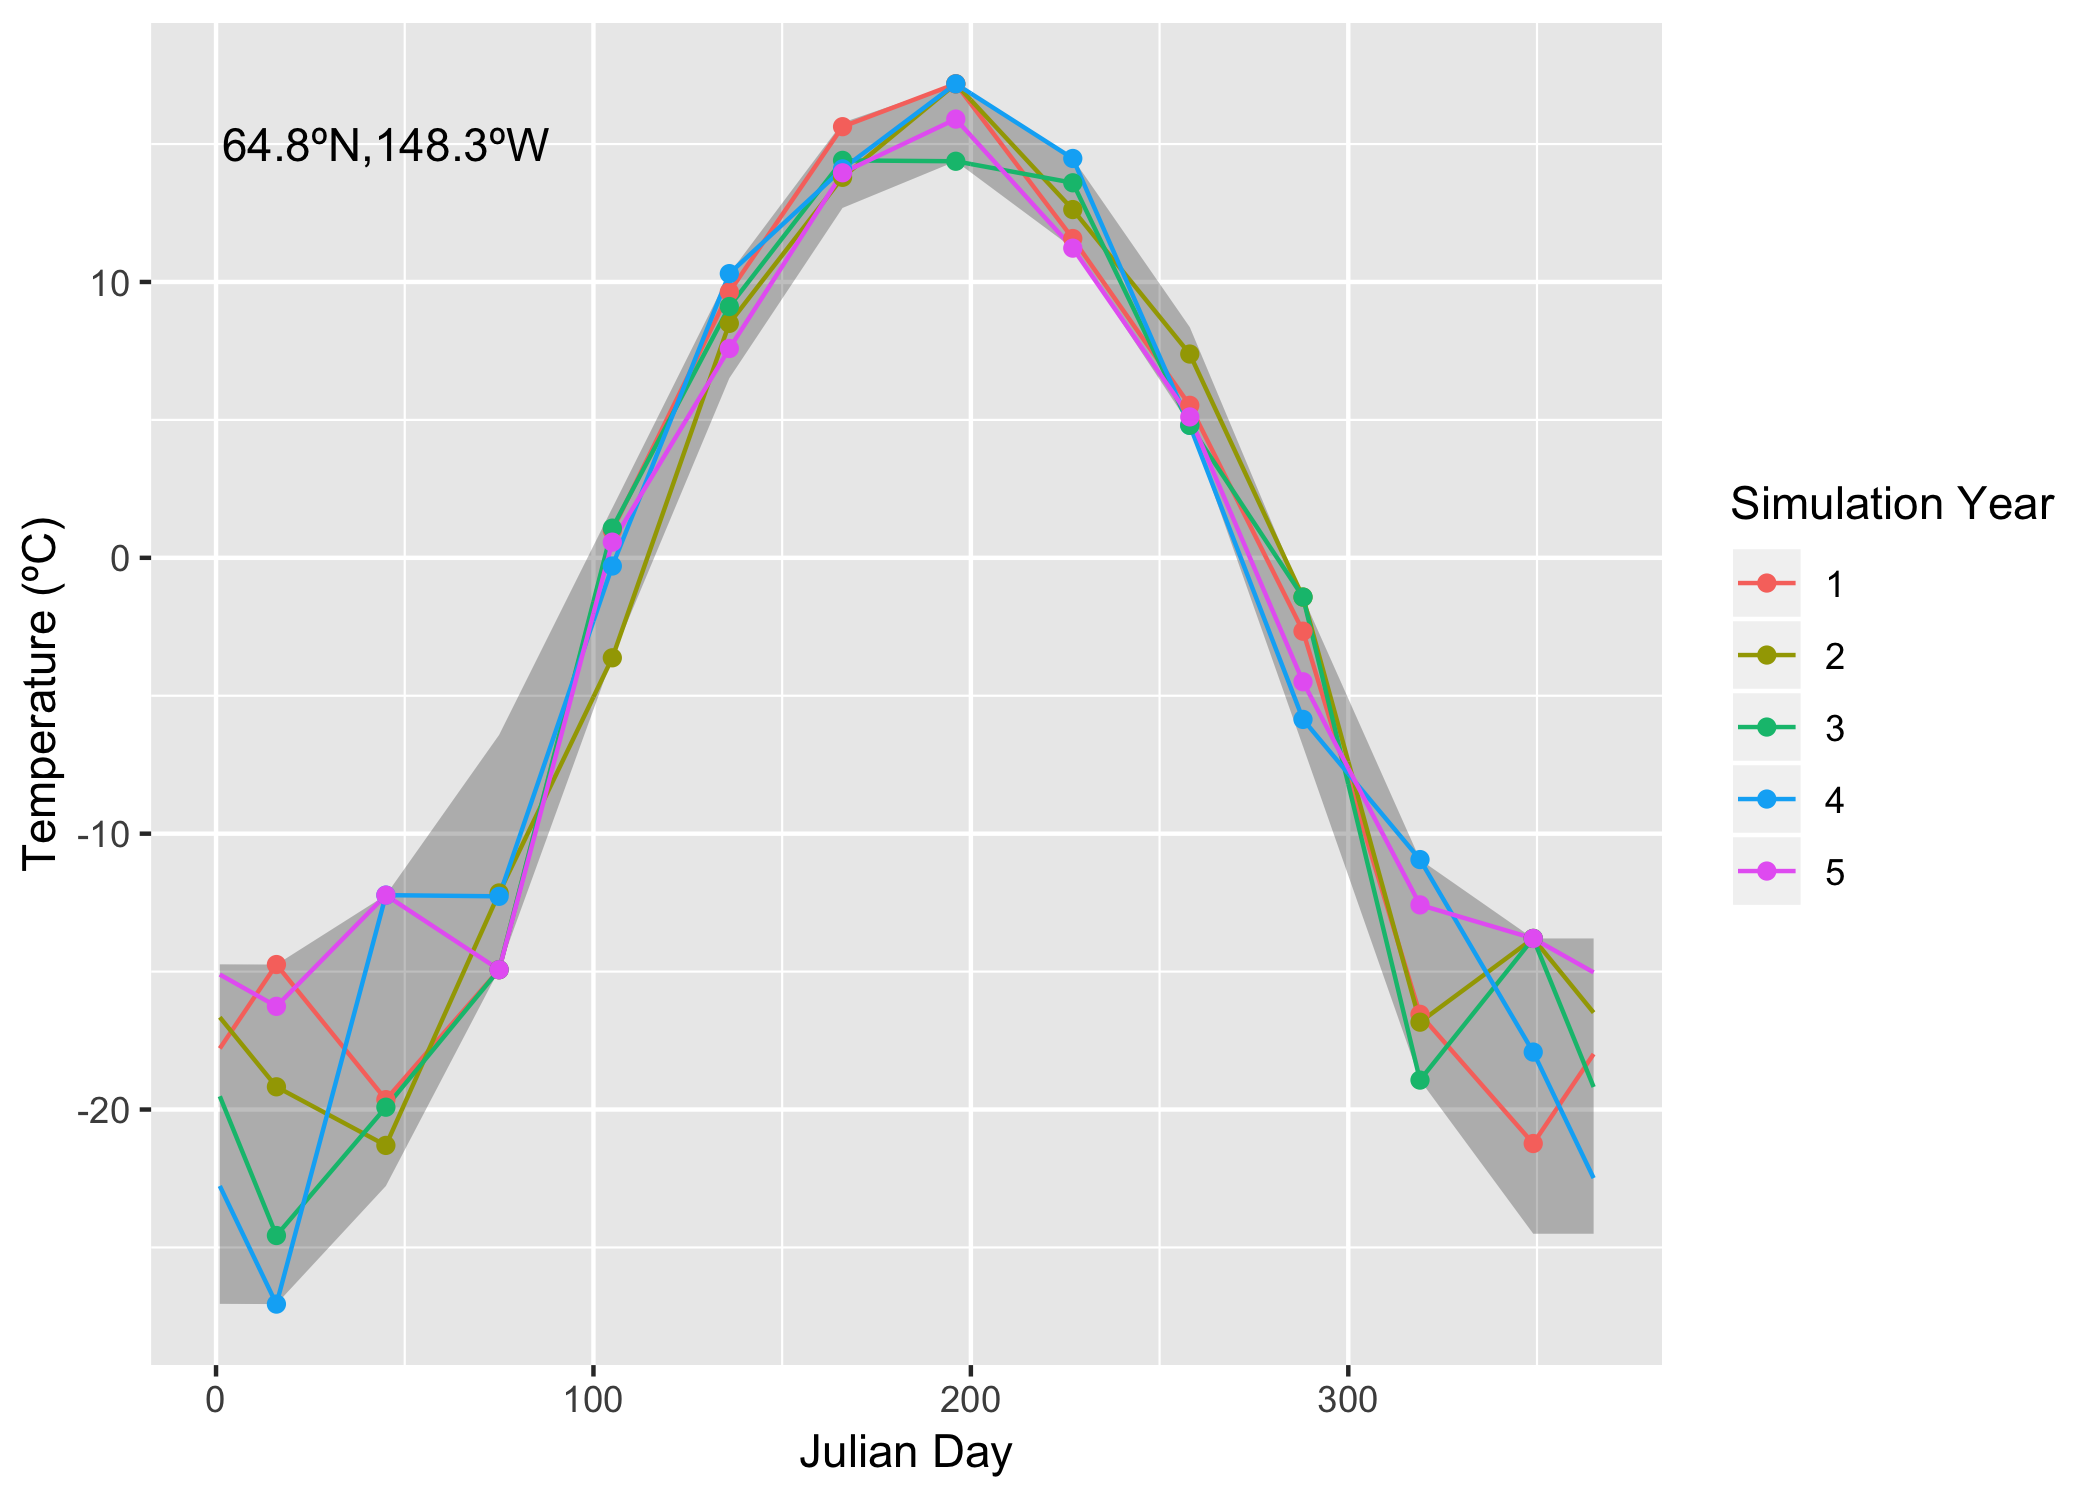
\includegraphics[width=0.78\linewidth]{Figures/Temperature_Daily.png}
  \caption{Example average monthly (points) and daily (lines) temperature (ºC) simulated by UVAFME for a site in interior Alaska. Shaded areas indicate the input mean $\pm$ standard deviation.}
  \label{fig:dailytemp}
\end{figure}

These monthly values are generated anew for each year of the simulation on each site and are equal across all plots within a site.

\subsubsection{Daily Weather Values}

The monthly simulated weather data are used to generate daily values for each year using a Gaussian approach (Fig. \ref{fig:dailytemp}). For temperature, cloud cover, and relative humidity, daily values are generated via:

\begin{equation}
v_d = v_m + \Big(\frac{v_{m+1} - v_m}{j_{m+1}-j_m}\Big)(j - j_m)
\end{equation}

where $v_d$ is the daily generated weather value (i.e. temperature, cloud cover, or relative humidity), $v_{m}$ and $v_{m+1}$ are the mean monthly value for the current and following months, $j$ is the Julian day, and $j_m$ and $j_{m+1}$ are the Julian days corresponding to the middle of the current and following months. For days in December, monthly means from January of that year are used for the ``following'' month.

To generate daily precipitation values, the monthly precipitation is used to calculate the number of days it rains that month (Fig. \ref{fig:raindays}), and the amount of rainfall for each rain day (Fig. \ref{fig:dailyprecip}). Rain days per month ($d_r$, Fig. \ref{fig:raindays}) is calculated as:

\begin{equation}\label{rd}
d_r = \min{(25, \frac{p_m}{4.0} + 1.0)}
\end{equation}

\begin{figure}
  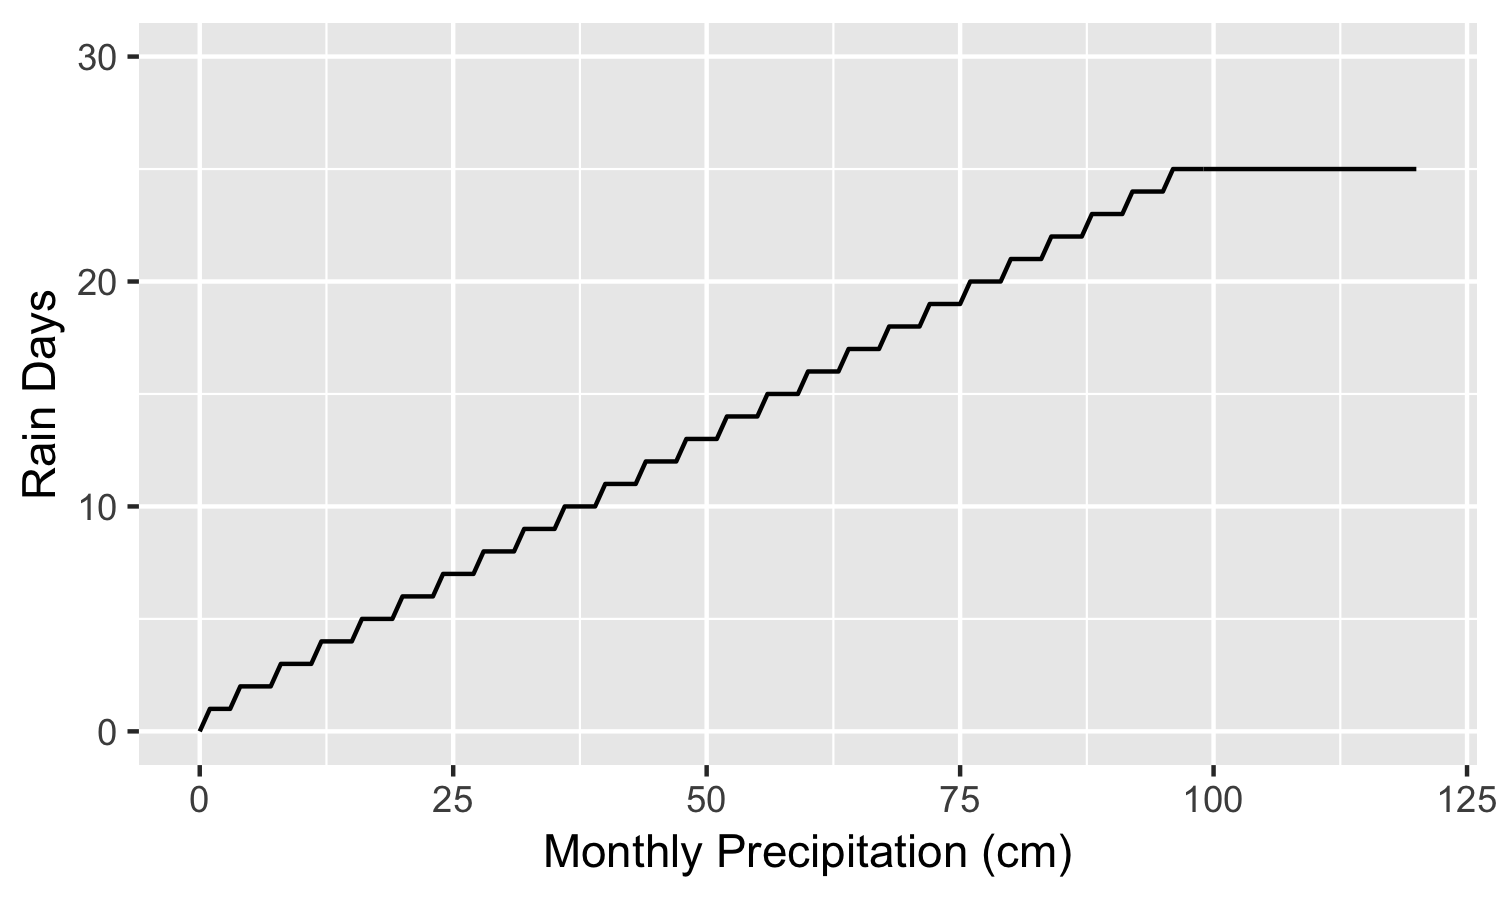
\includegraphics[width=0.58\textwidth]{Figures/RainDays.png}
  \caption{Number of rain days for a month based on monthly precipitation (cm) (Eq. \ref{rd}).}
  \label{fig:raindays}
\end{figure}

Monthly rain days are distributed across the days in the month until all rain days have been used. Starting from the first of each month, if the number of rain days is greater than 0, a uniformly distributed random number between 0.0 and 1.0 is generated ($u_r$; Section \ref{random}). If this number is less than or equal to the percent of rain days that month (i.e. $u_r \leq{\frac{d_r}{d_m}}$, where $d_m$ is the number of days in the month), then the amount of rainfall for that day is set as $\frac{p_m}{d_r}$, otherwise no rainfall occurs that day. Once the number of rain days in the month have been assigned, all subsequent days in the month have no rainfall.

\begin{figure}
  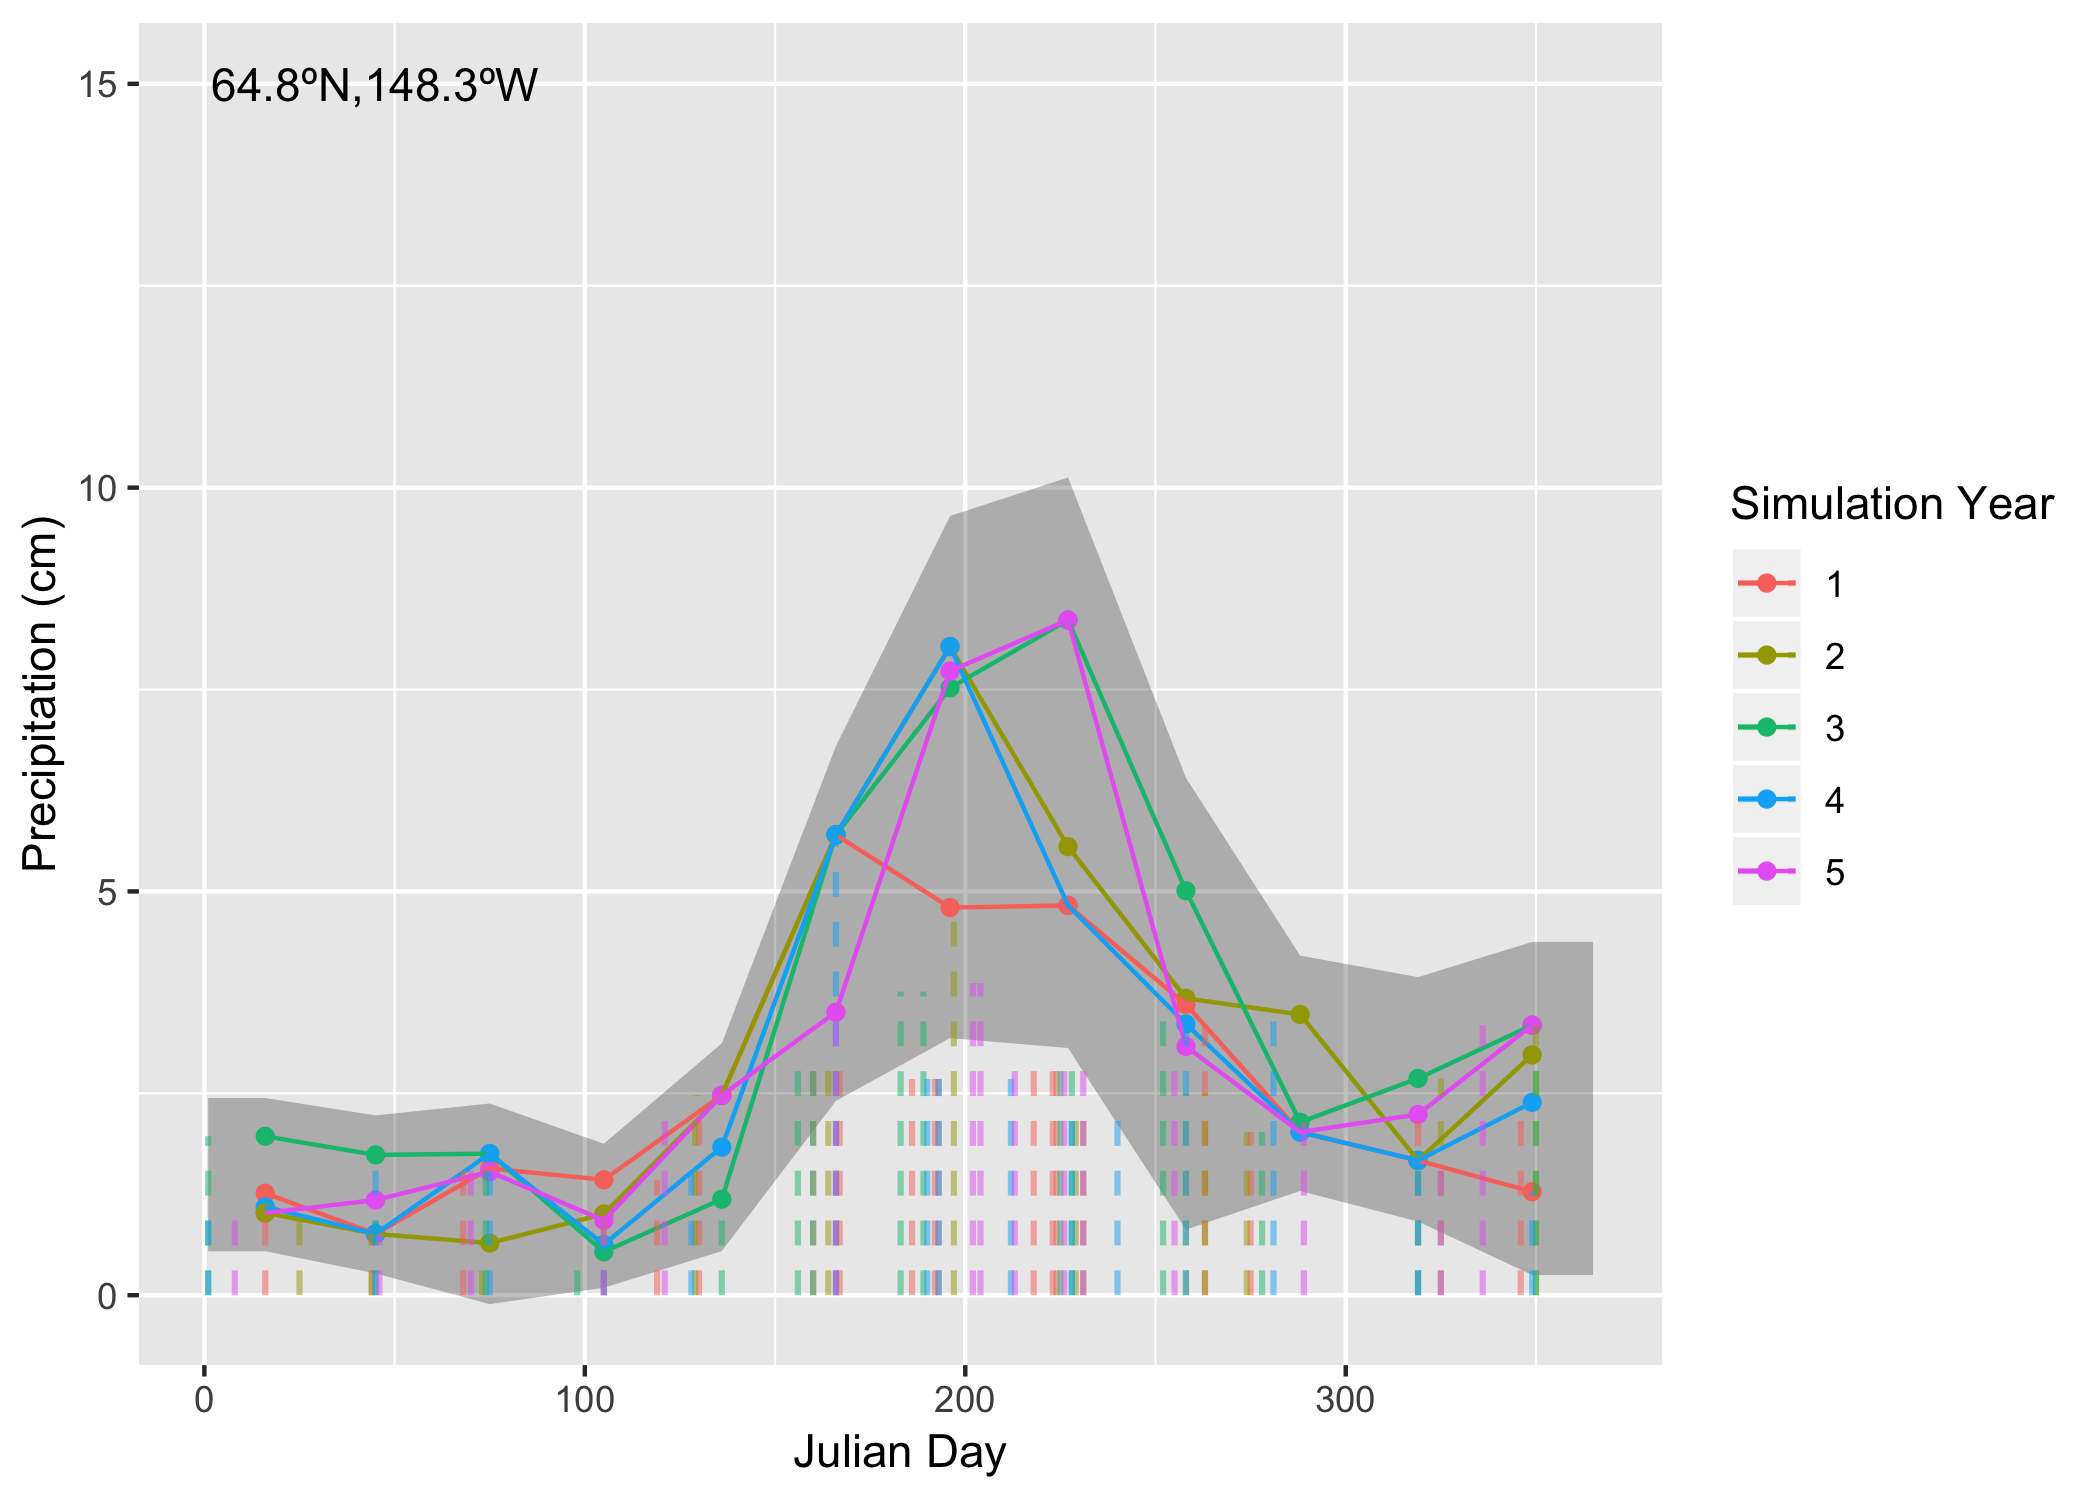
\includegraphics[width=0.8\linewidth]{Figures/Precipitation_Daily.png}
  \caption{Example monthly (solid) and daily (dashed) precipitation (cm) simulated by UVAFME for a site in interior Alaska. Shaded areas indicate the input mean $\pm$ standard deviation.}
  \label{fig:dailyprecip}
\end{figure}

\subsubsection{Hourly Temperature Values}
Hourly temperatures can also be calculated via a sinusoidal formula from \shortcite{reicoskyAccuracyHoulyAir1989}. This formulation is based on daily minimum, maximum, and mean temperatures ($t_{min}$, $t_{max}$, and $t_{mean} = (t_{max} + t_{min})/2$) as well as sunrise hour ($h_{rise}$). Hourly temperature ($t_h$, ºC) is calculated as:

\begin{equation}\label{hourlytemp}
t_h=\begin{cases}
	t_{mean} + \frac{t_{max} - t_{min}}{2}\cos{(\frac{\pi (h + 10)}{10 + h_{rise}})}, & \text{$0 \leq h < h_{rise}$} \\
	t_{mean} -  \frac{t_{max} - t_{min}}{2}\cos{(\frac{\pi (h - h_{rise})}{h_{max} - h_{rise}})}, & \text{$h_{rise} \leq h \leq h_{max}$} \\
	t_{mean} + \frac{t_{max} - t_{min}}{2}\cos{(\frac{\pi (h + h_{max})}{10 + h_{rise}})}, & \text{$h_{max} < h \leq 24$}
  \end{cases}
\end{equation}

where $h_{max}$ is the hour of maximum temperature, currently set to a default of 14 across all sites and year. Sunrise hour is calculated in the solar radiation subroutine (see Section \ref{solar}) (Fig. \ref{fig:htemp}).

\begin{figure}
  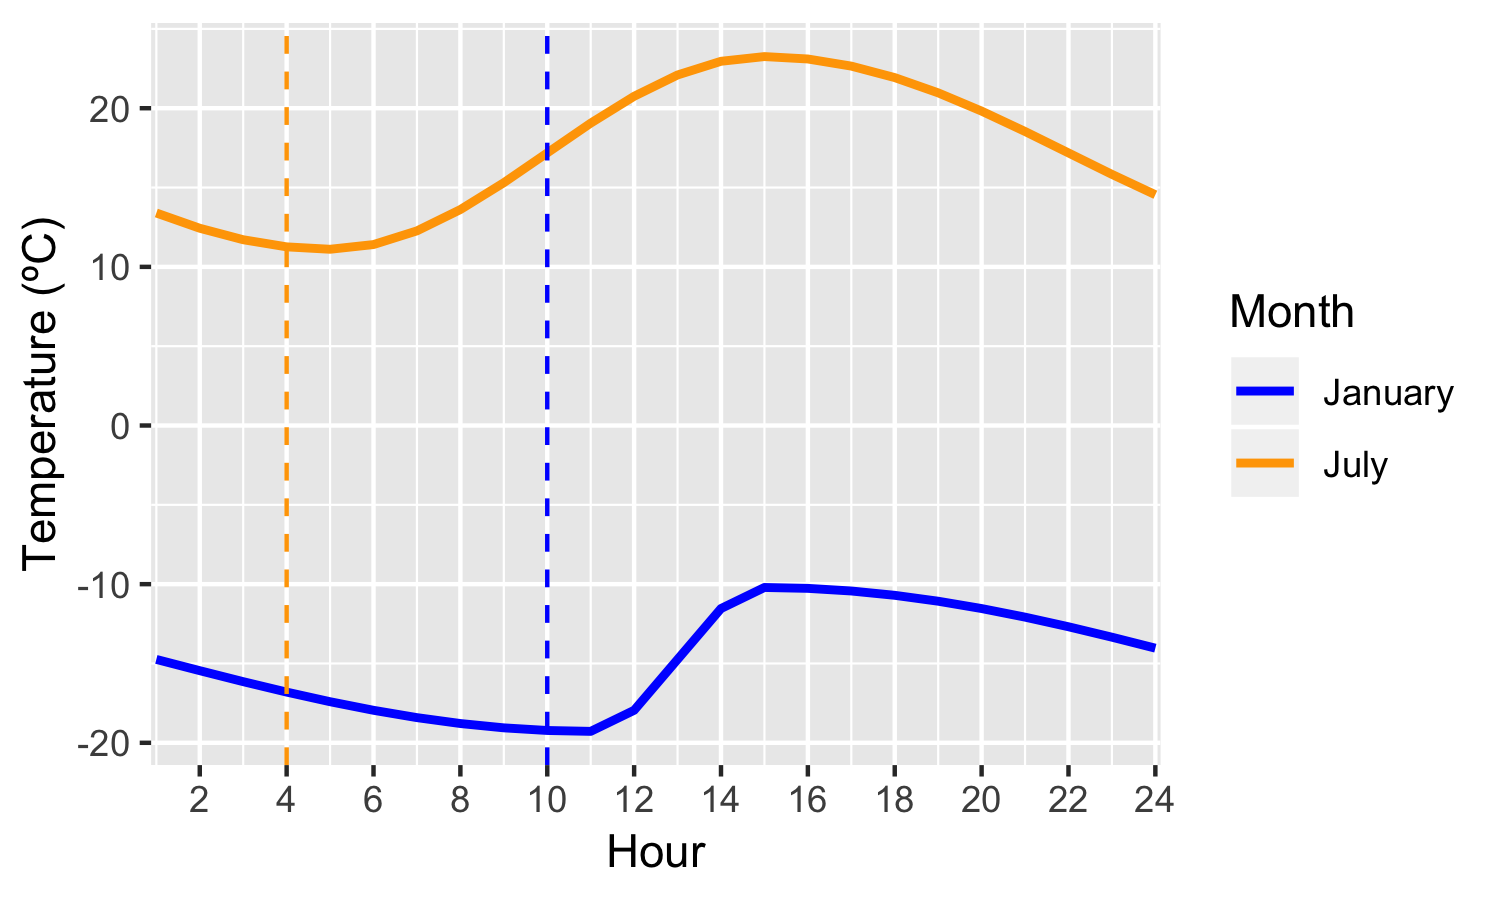
\includegraphics[width=0.8\linewidth]{Figures/HourlyTemp.png}
  \caption{Example hourly temperature (ºC) for a site in interior Alaska on a typical day in mid-January ($t_{min} = -19$ºC, $t_{max} = -10$ºC) and mid-July ($t_{min} = 11$ºC, $t_{max} = 23$ºC). Dashed lines show time of sunrise.}
  \label{fig:htemp}
\end{figure}

\subsubsection{Climate Change}
Climate change can be prescribed either linearly or via an input climate change file. Climate change, in the form of changing mean monthly temperatures, precipitation, and relative humidity, is achieved by modifying the input values of average monthly minimum and maximum temperatures ($\bar{t}_{min}$ and $\bar{t}_{max}$), precipitation ($\bar{p}_m$), and relative humidity ($\bar{RH}_m$) for a simulated site. 

For linear climate change, total input temperature and/or precipitation change ($t_c$, ºC or $p_c$, percent change, 0 to 1) is applied over an input duration ($y_c$, years) such that the amount of change per year is calculated as $t' = \frac{t_c}{y_c + 1}$ and $p' = \frac{p_c}{y_c + 1}$. Currently changes in relative humidity are only available via an input climate change file (see below). 

When climate change starts in the model, the initial minimum and/or maximum temperatures are modified each year for the duration of the climate change application via $\bar{t}_m = \bar{t}_m + t'$. Likewise, the initial monthly precipitation values are modified each year for the duration of climate change application via $\bar{p}_m = \bar{p}_m + \bar{p}_mp'$. These modifications continue for the duration of climate change, at which point the total change in temperature or precipitation will have occurred, and all variables stabilize at the new values of $\bar{t}_m + t_c$ and $\bar{p}_m + \bar{p}_mp_c$.

For non-linear climate change simulations, new mean monthly values for each year are read in from an input climate change file.

Currently, all cloudiness variables and all monthly standard deviations do not change from the historical inputs during the climate change application.

\subsubsection{Elevational Change}
Often it is beneficial to run the model at the same site latitude and longitude, but at different elevations (such as in studies in complex terrain or for testing applications). Both temperature and precipitation change as altitude/elevation changes. These changes can be generated in UVAFME using input values of the base site elevation, the new elevation, and temperature and precipitation lapse rates. As with climate change, these modifications are made to the initial input average minimum and maximum temperatures and precipitation for a particular site. Temperature and precipitation are modified as:

\begin{equation}
\bar{t}_m = \bar{t}_m - 0.01(E' - E)t_l
\end{equation}

\begin{equation}
\bar{p}_m = \max{(\bar{p}_m + 0.001(E' - E)p_l, 0.0)}
\end{equation}

where $E'$ is the new elevation at which the model is to be run (m), $E$ is the original elevation at which the input climate data were derived (m), $t_l$ is the input temperature lapse rate (ºC km$^{-1}$), and $p_l$ is the input precipitation lapse rate (mm km$^{-1}$).

\subsection{Solar Radiation} \label{solar}
Daily and annual solar radiation is used to calculate potential evapotranspiration (PET) (Section \ref{pet}) and permafrost dynamics (Section \ref{perm}) within UVAFME. Previous versions of the model used top-of-atmosphere solar radiation to derive PET \cite{fosterValidationApplicationForest2017}, however as of Version 3, surface solar radiation is used to account for the effects of slope, aspect, and cloud cover on solar radiation received at a surface (Fig. \ref{fig:solardiagram}). 

\begin{figure}
  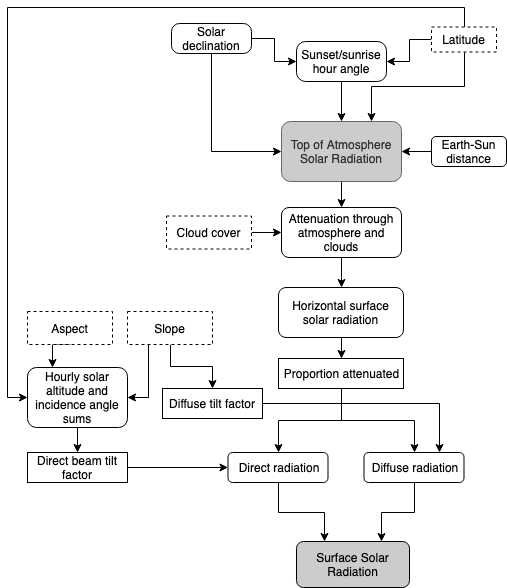
\includegraphics[width=0.7\linewidth]{Figures/SolarRadiation.png}
  \caption{Flow diagram showing how solar radiation is calculated in UVAFME.}
  \label{fig:solardiagram}
\end{figure}

\subsubsection{Top-of-Atmosphere Radiation}

Top-of-atmosphere solar radiation (cal cm$^{-2}$ day$^{-1}$) is calculated as a function of latitude, solar declination, relative Earth-Sun distance, and sunrise/sunset hour angle \cite{brockCalculatingSolarRadiation1981}. The eccentricity of Earth's orbit around the Sun causes the Earth-Sun distance to vary by $\sim$3\% throughout a single revolution \cite{brockCalculatingSolarRadiation1981} (Fig. \ref{fig:esdist}). Such variation affects the amount of solar radiation received by the Earth throughout the year. The relative Earth-Sun distance ($r_{ES}$, in AU; 1 AU = 1.485$\times$10$^{11}$ m) for day of year $j$ can be calculated as \cite{brockCalculatingSolarRadiation1981, nichollsSolarRadiationCharts1979} (Fig. \ref{fig:esdist}):

\begin{figure}
  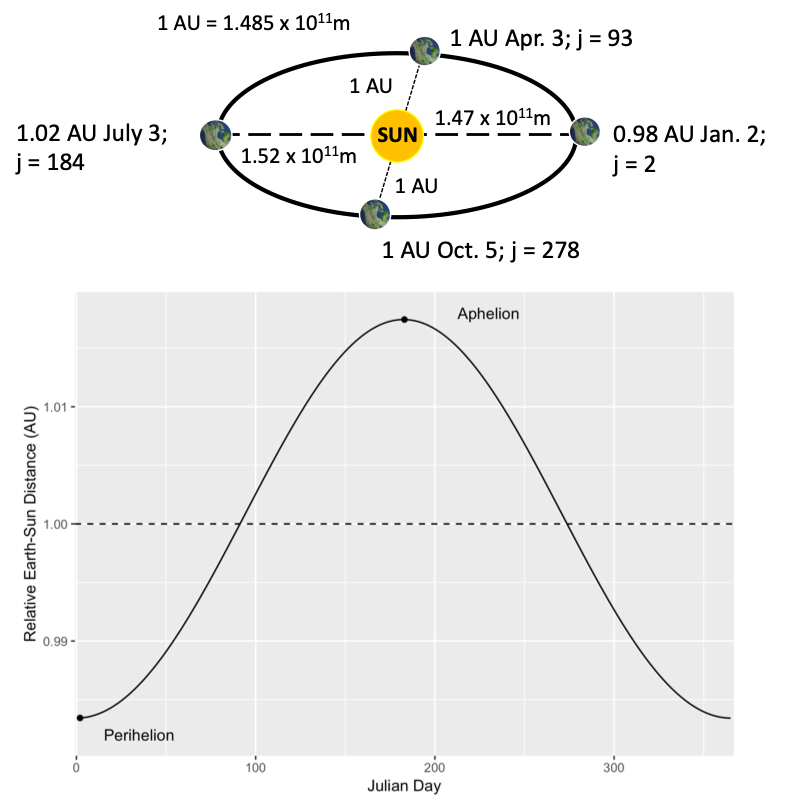
\includegraphics[width=0.75\linewidth]{Figures/Earth_Sun_Distance.png}
  \caption{The Earth-Sun distance varies throughout the year due to the Earth's orbital eccentricity (Eq. \ref{esr})}
  \label{fig:esdist}
\end{figure}

\begin{equation}\label{esr}
r_{ES} = \Big(1.0 + 0.033\cos{(0.017214j)}\Big)^{-1/2}
\end{equation}

Solar declination is the angular distance at solar noon between the Sun and the Equator (north-positive) and affects the solar radiation received at the top of the atmosphere. Earth is tilted at 23.4º from its plane of orbit. As the Earth revolves around the Sun, the solar declination changes such that at the spring and autumn equinoxes ($j =$ 80 and 264) the Sun shines equally in both hemispheres and the declination is 0º. At the summer and winter solstices ($j=$ 173 and 356) the Sun is directly overhead at 23.45ºN and 23.45ºS, respectively \cite{brockCalculatingSolarRadiation1981} (Fig. \ref{fig:decl}).

\begin{figure}
  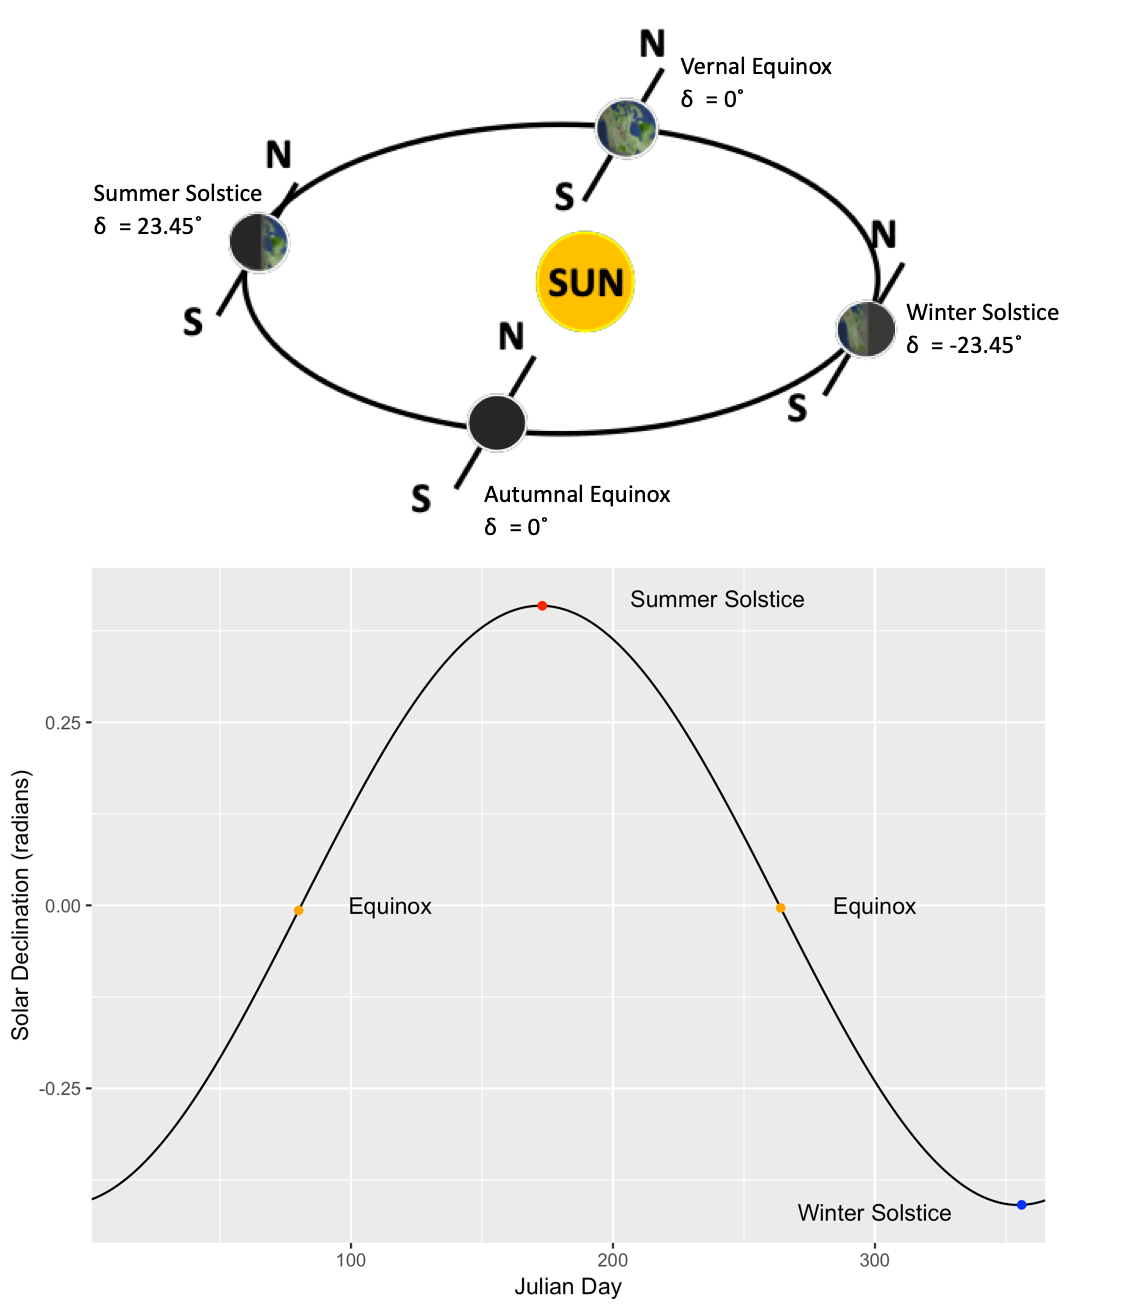
\includegraphics[width=0.75\linewidth]{Figures/Solar_Declination.png}
  \caption{Declination varies throughout the year impacting top-of-atmosphere radiation (Eq. \ref{declin})}
  \label{fig:decl}
\end{figure}

Solar declination ($\delta$, radians) can be calculated using an equation from Cooper (1969):

\begin{equation}\label{declin}
\delta = 23.45\sin{(\frac{284 + j}{365}2\pi)}\frac{\pi}{180}
\end{equation}

Finally, sunset/sunrise hour angle is used to account for the daily rotation of Earth around itself. Sunset/sunrise hour-angle is the angle between the setting/rising Sun and the south point. This angle depends on declination as well as latitude on Earth, and can be calculated as \cite{brockCalculatingSolarRadiation1981} :

\begin{equation}\label{hourangle}
\cos{\omega} = -\tan{\phi}\tan{\delta}
\end{equation}

where $\omega$ is the sunset/sunrise hour angle (radians), and $\phi$ is the site's latitude (radians). When $\tan{\phi}\tan{\delta} > 1.0$ the sun never sets, and the sunset/sunrise angle is set to $\pi$. When $\tan{\phi}\tan{\delta} < -1.0$ the sun never rises above the horizon and the sunset/sunrise angle is set to 0 \cite{keithPrinciplesSolarEngineering1978} (Fig. \ref{fig:sunset}).

\begin{figure}
  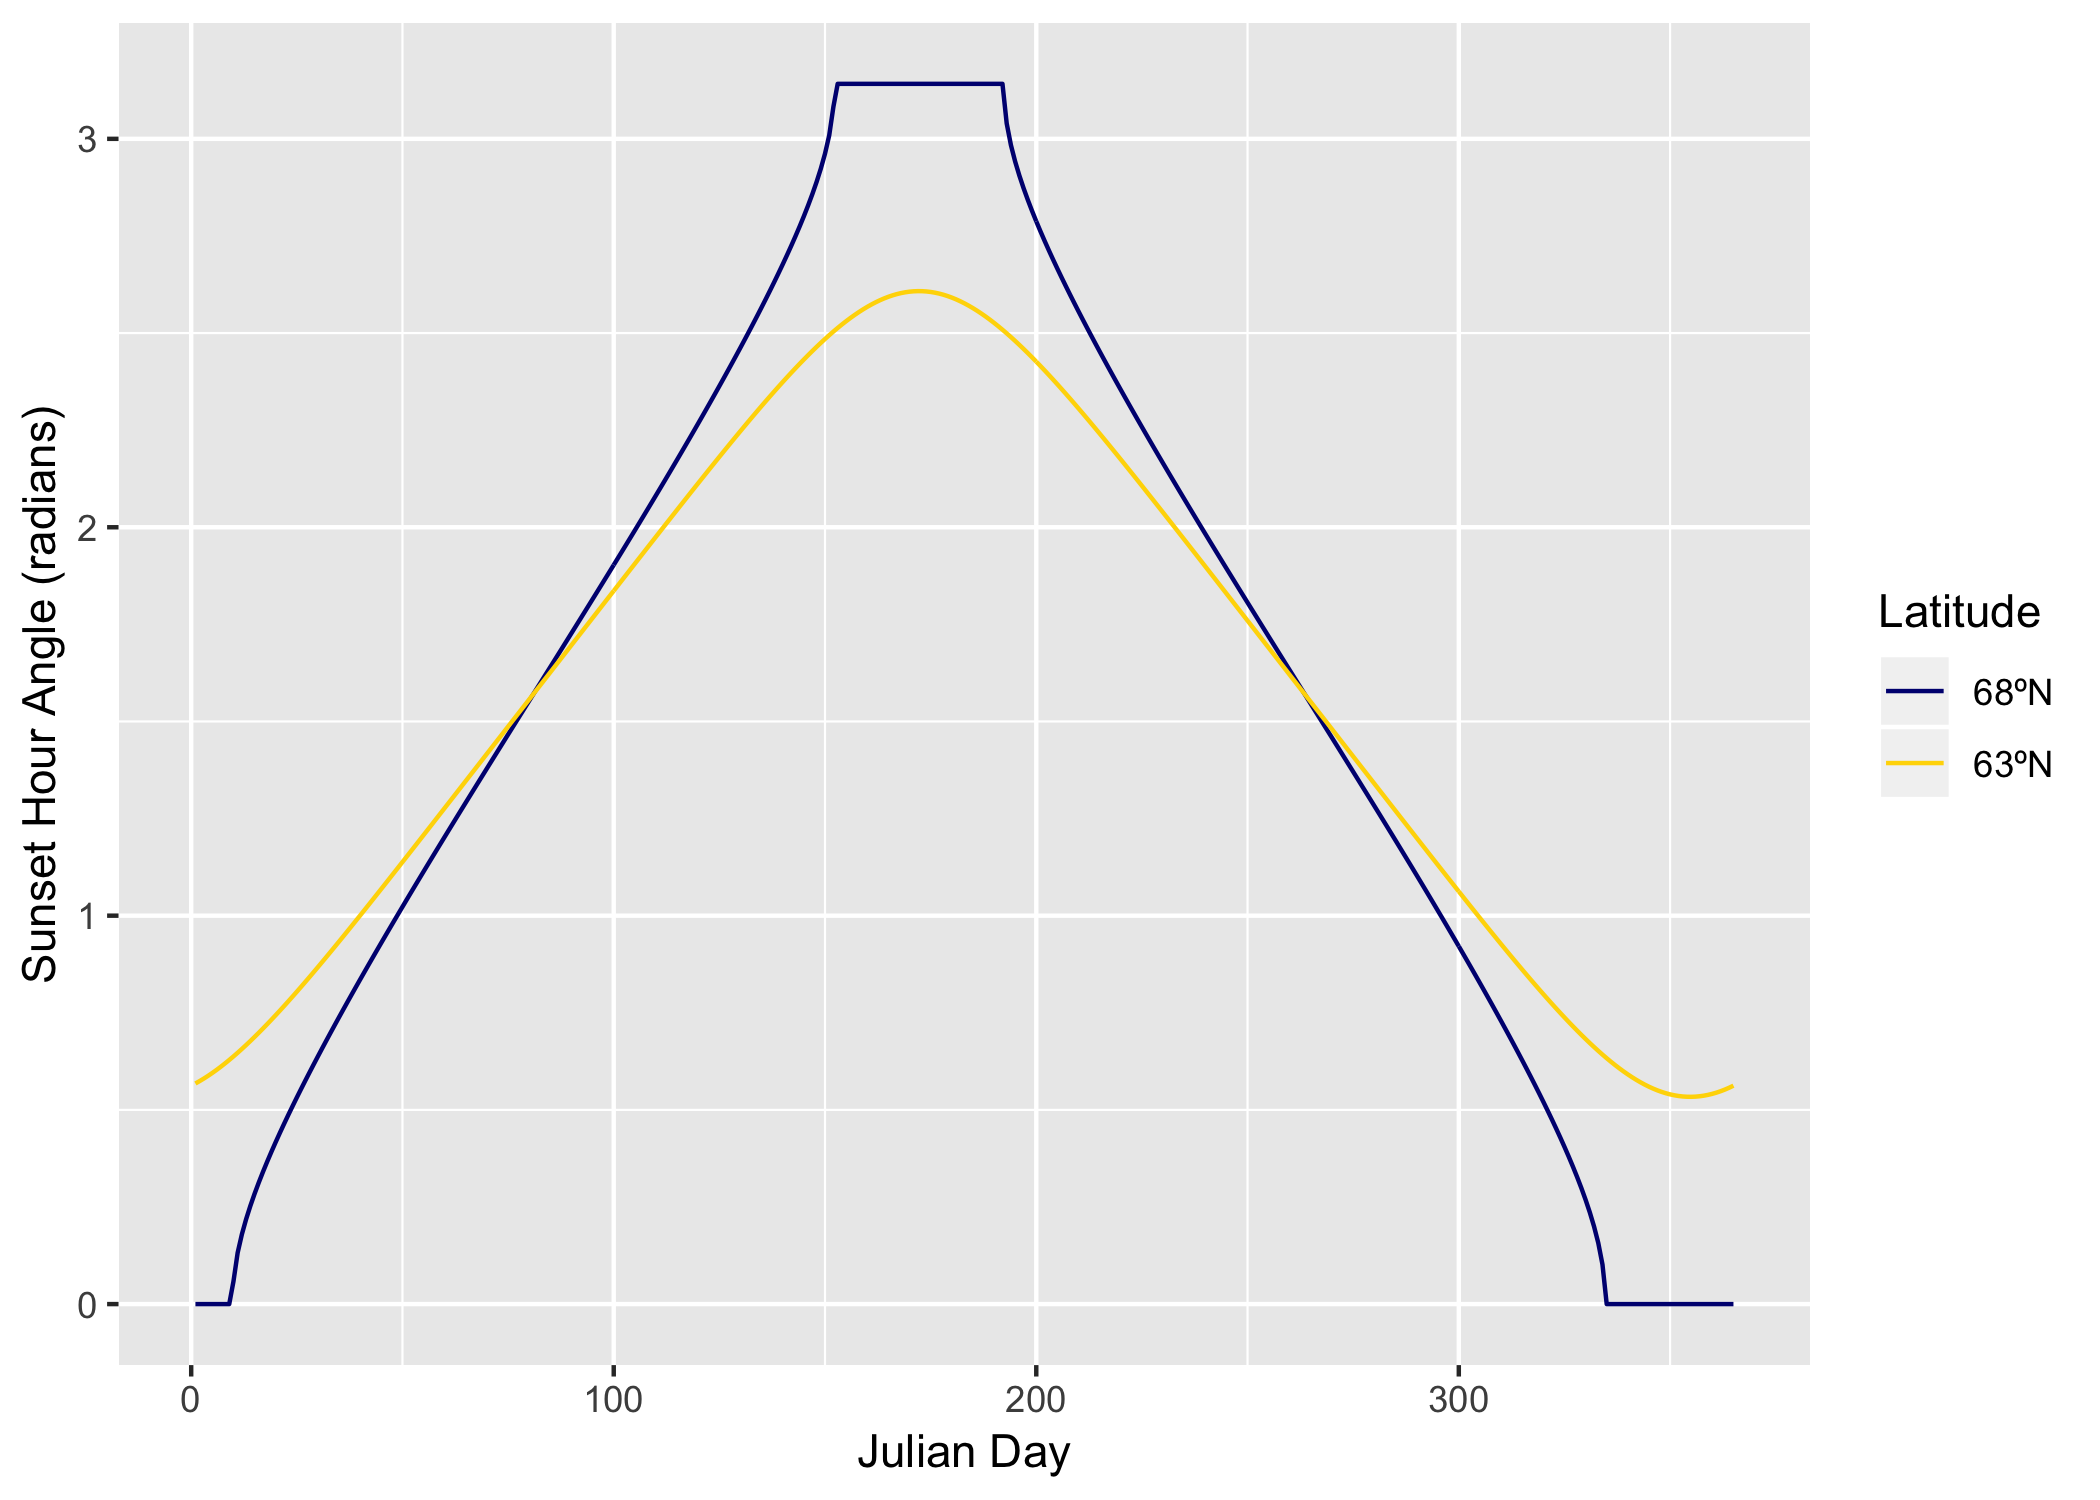
\includegraphics[width=0.75\linewidth]{Figures/SunsetHourAngle.png}
  \caption{Example sunset hour angle calculation for two sites in interior Alaska (Eq. \ref{hourangle})}
  \label{fig:sunset}
\end{figure}

Top-of-atmosphere solar radiation is then calculated as \cite{kleinCalculationMonthlyAverage1977}:

\begin{equation}\label{Srad}
R_{toa} = \frac{S}{\pi}\frac{1}{{r_{ES}}^2}\cos{(\phi)}\cos{(\delta)}\Big(\sin{(\omega)} - \omega\cos{(\omega)}\Big)
\end{equation}

where $R_{toa}$ is the solar radiation received at the top of the Earth's atmosphere (cal cm$^{-2}$ day$^{-1}$) and $S$ is the solar constant (2880 cal cm$^{-2}$ day$^{-1}$) (Fig. \ref{fig:toa}).

\begin{figure}[H]
  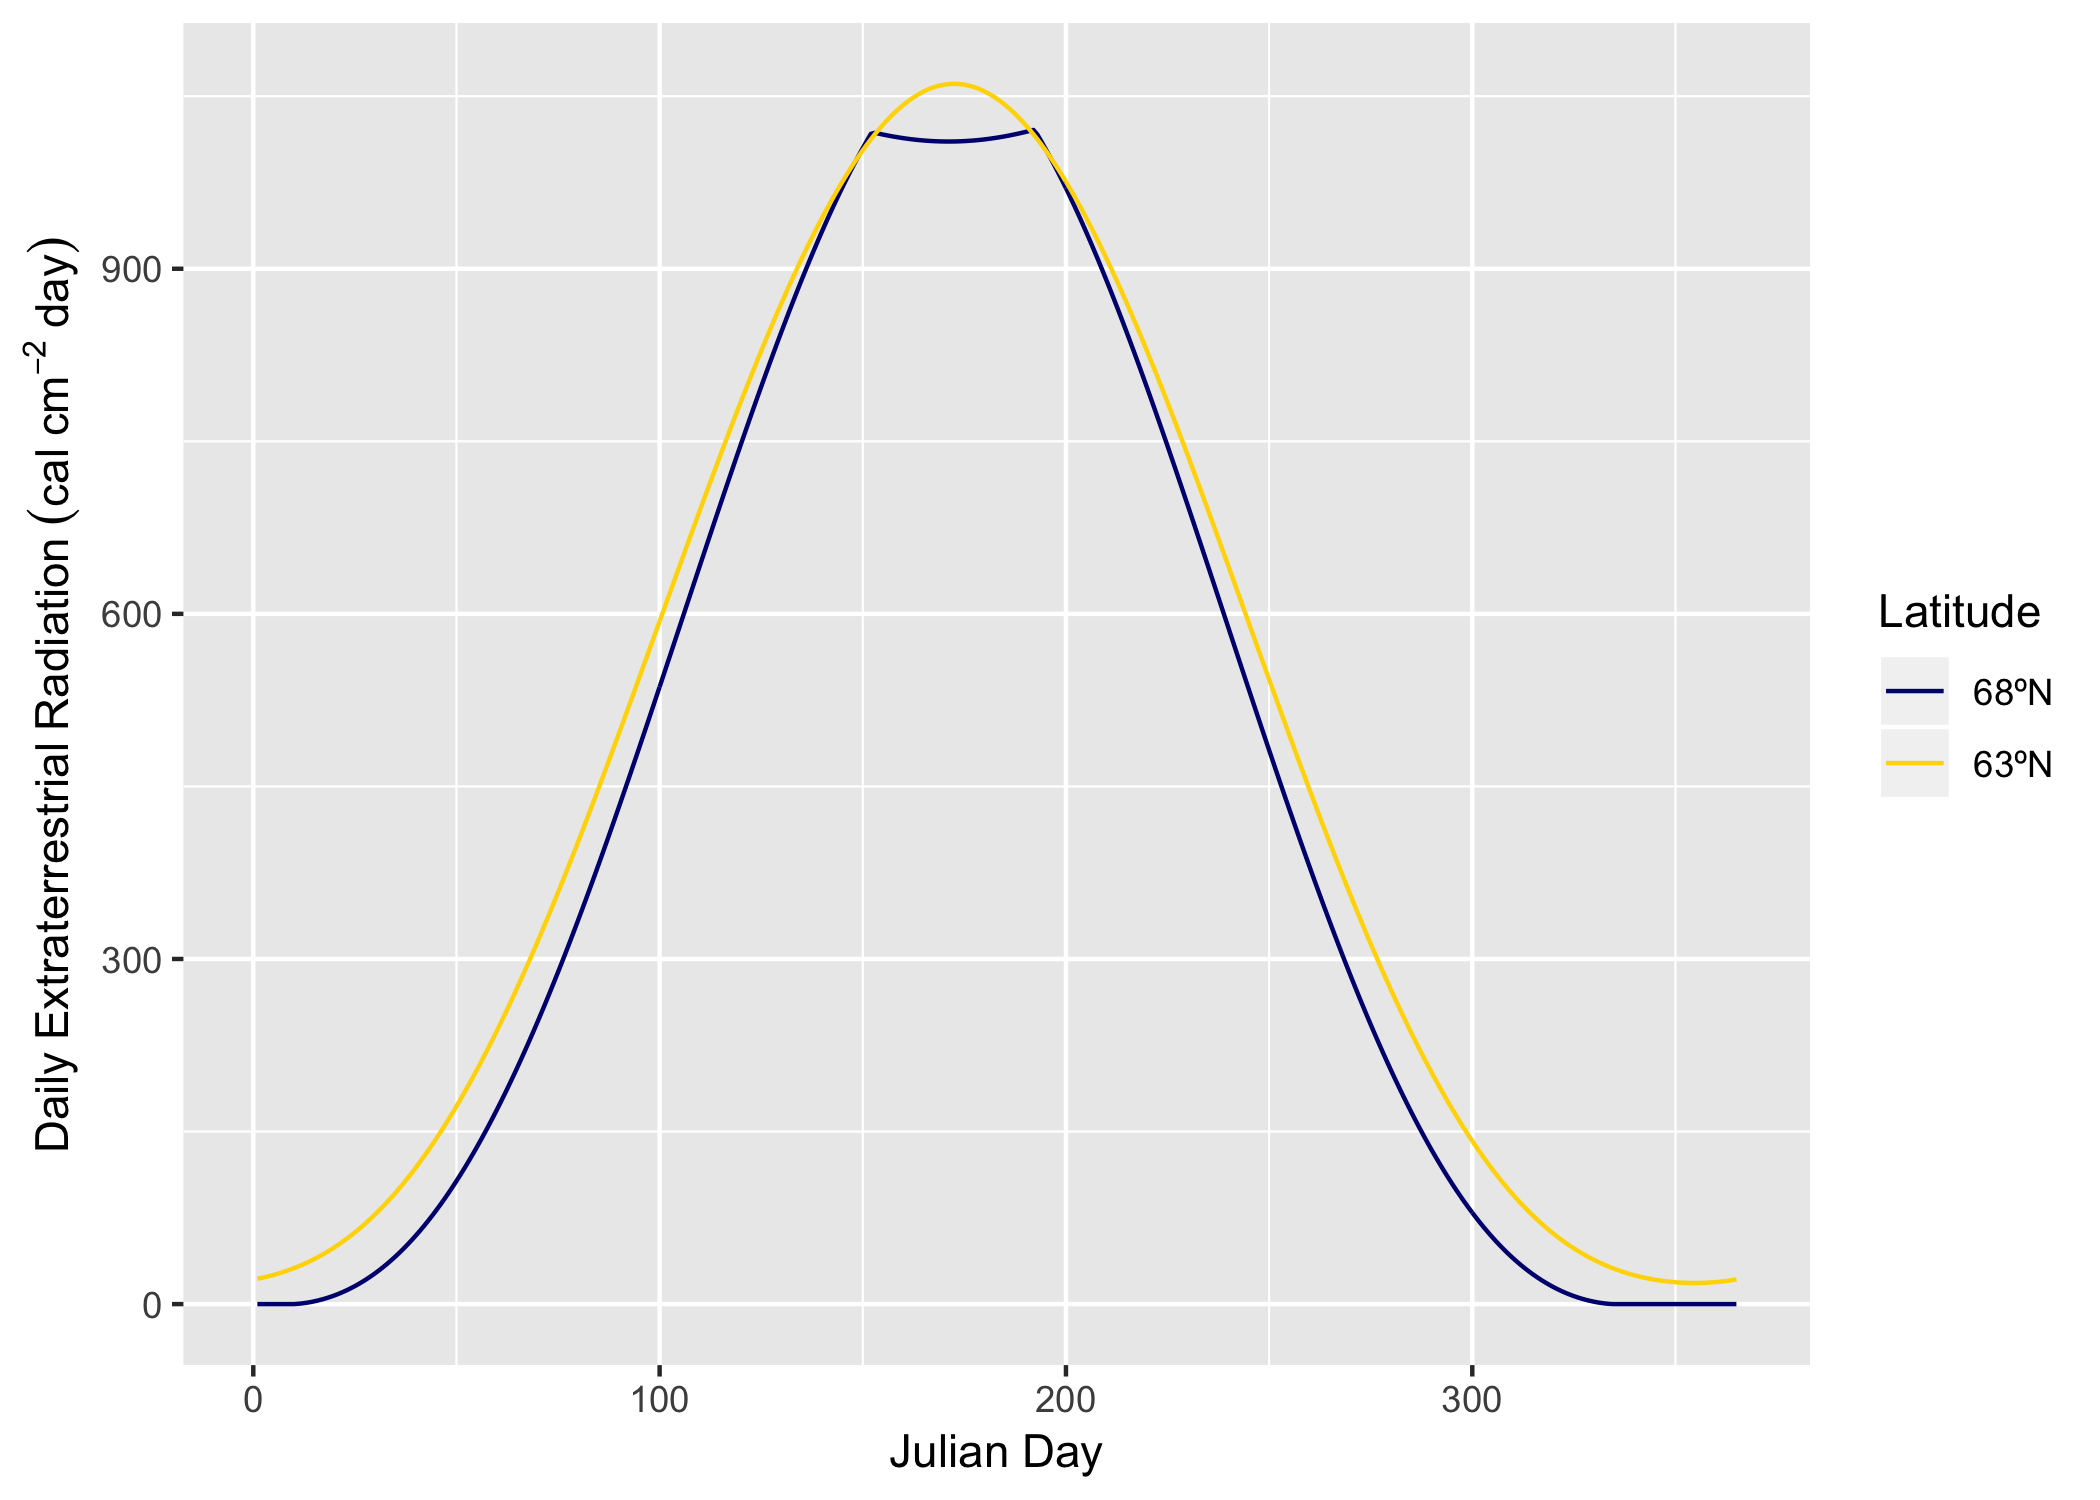
\includegraphics[width=0.75\linewidth]{Figures/SolarRad_toa.png}
  \caption{Example TOA solar radiation calculation for two sites in interior Alaska  (Eq. \ref{Srad})}
  \label{fig:toa}
\end{figure}

\subsubsection{Surface Radiation}
Top-of-atmosphere solar radiation is first attenuated through the atmosphere and clouds using an equation from \citeA{bonanComputerModelSolar1989} (Eq. \ref{cld}). Bonan developed linear regressions of data from meteorological stations across North America, Scandinavia, and Russia on solar radiation and cloud cover (Fig. \ref{fig:cld_eq}).

\begin{equation} \label{cld}
R_{H} = s_1 + s_2R_{toa} - s_3R_{toa}(c/10)
\end{equation}

\begin{figure}
  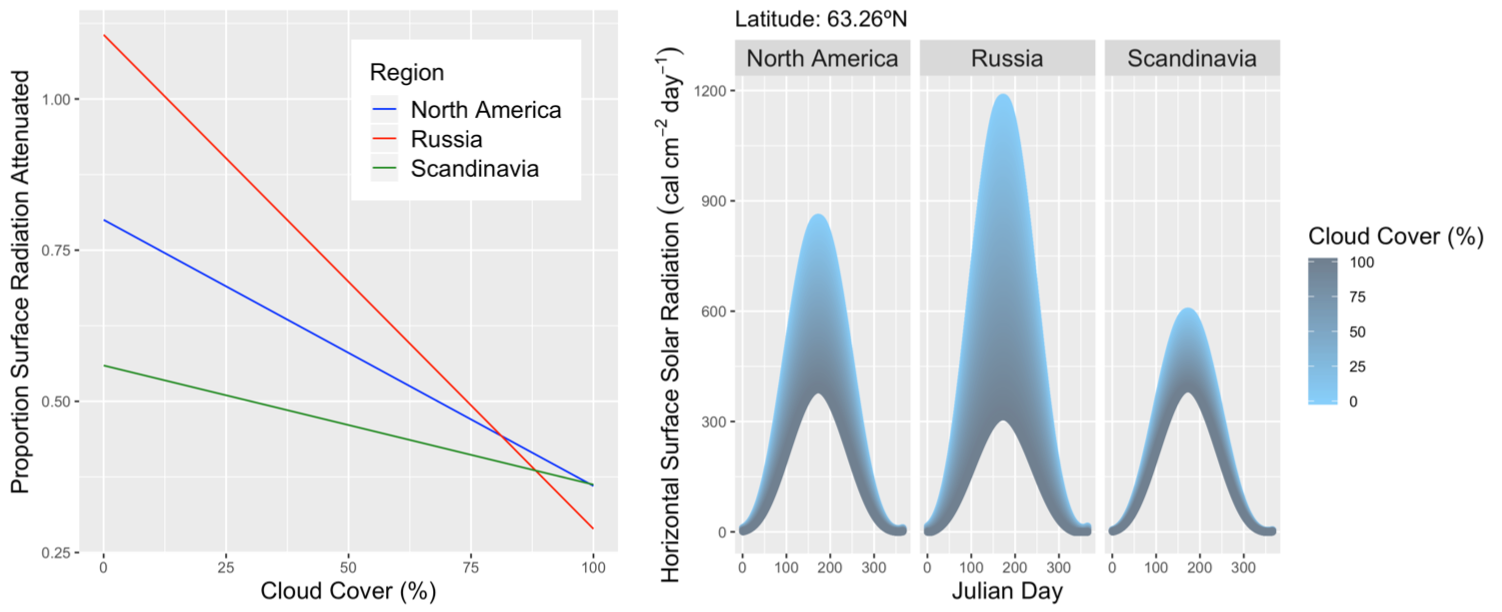
\includegraphics[width=\linewidth]{Figures/Cloud_Cover.png}
  \caption{Left: linear regressions for attenuating top-of-atmosphere solar radiation through the atmosphere and clouds. Right: Example attenuated radiation at the same latitude for different levels of cloud cover for the three regions modeled in \protect\citeA{bonanComputerModelSolar1989} (Eq. \ref{cld}).}
  \label{fig:cld_eq}
\end{figure}

where $R_H$ is surface solar radiation (cal cm$^{-2}$ day$^{-1}$) received on a horizontal surface, $c$ is cloudiness (in tenths of sky covered), and $s_1$, $s_2$, and $s_3$ are parameters from \citeA{bonanComputerModelSolar1989}, with $s_1 = -7.130$, $s_2 = 0.812$, and $s_3 = 0.440$ for North America. This surface radiation is partitioned into direct and diffuse radiation using equations from \citeA{keithPrinciplesSolarEngineering1978} (Fig. \ref{fig:KK}). Horizontal diffuse radiation ($R_{Hd}$, cal cm$^{-2}$ day$^{-1}$) is calculated as:

\begin{equation} \label{kk}
R_{Hd}=\begin{cases}
	\Big(1.0045 + 0.04349K_t - 3.5227{K_t}^2 + 2.6313{K_t}^3\Big)R_H, & \text{$K_t \leq 0.75$}.\\
	0.166R_H, & \text{$K_t > 0.75$}.
  \end{cases}
\end{equation}

\begin{figure}
  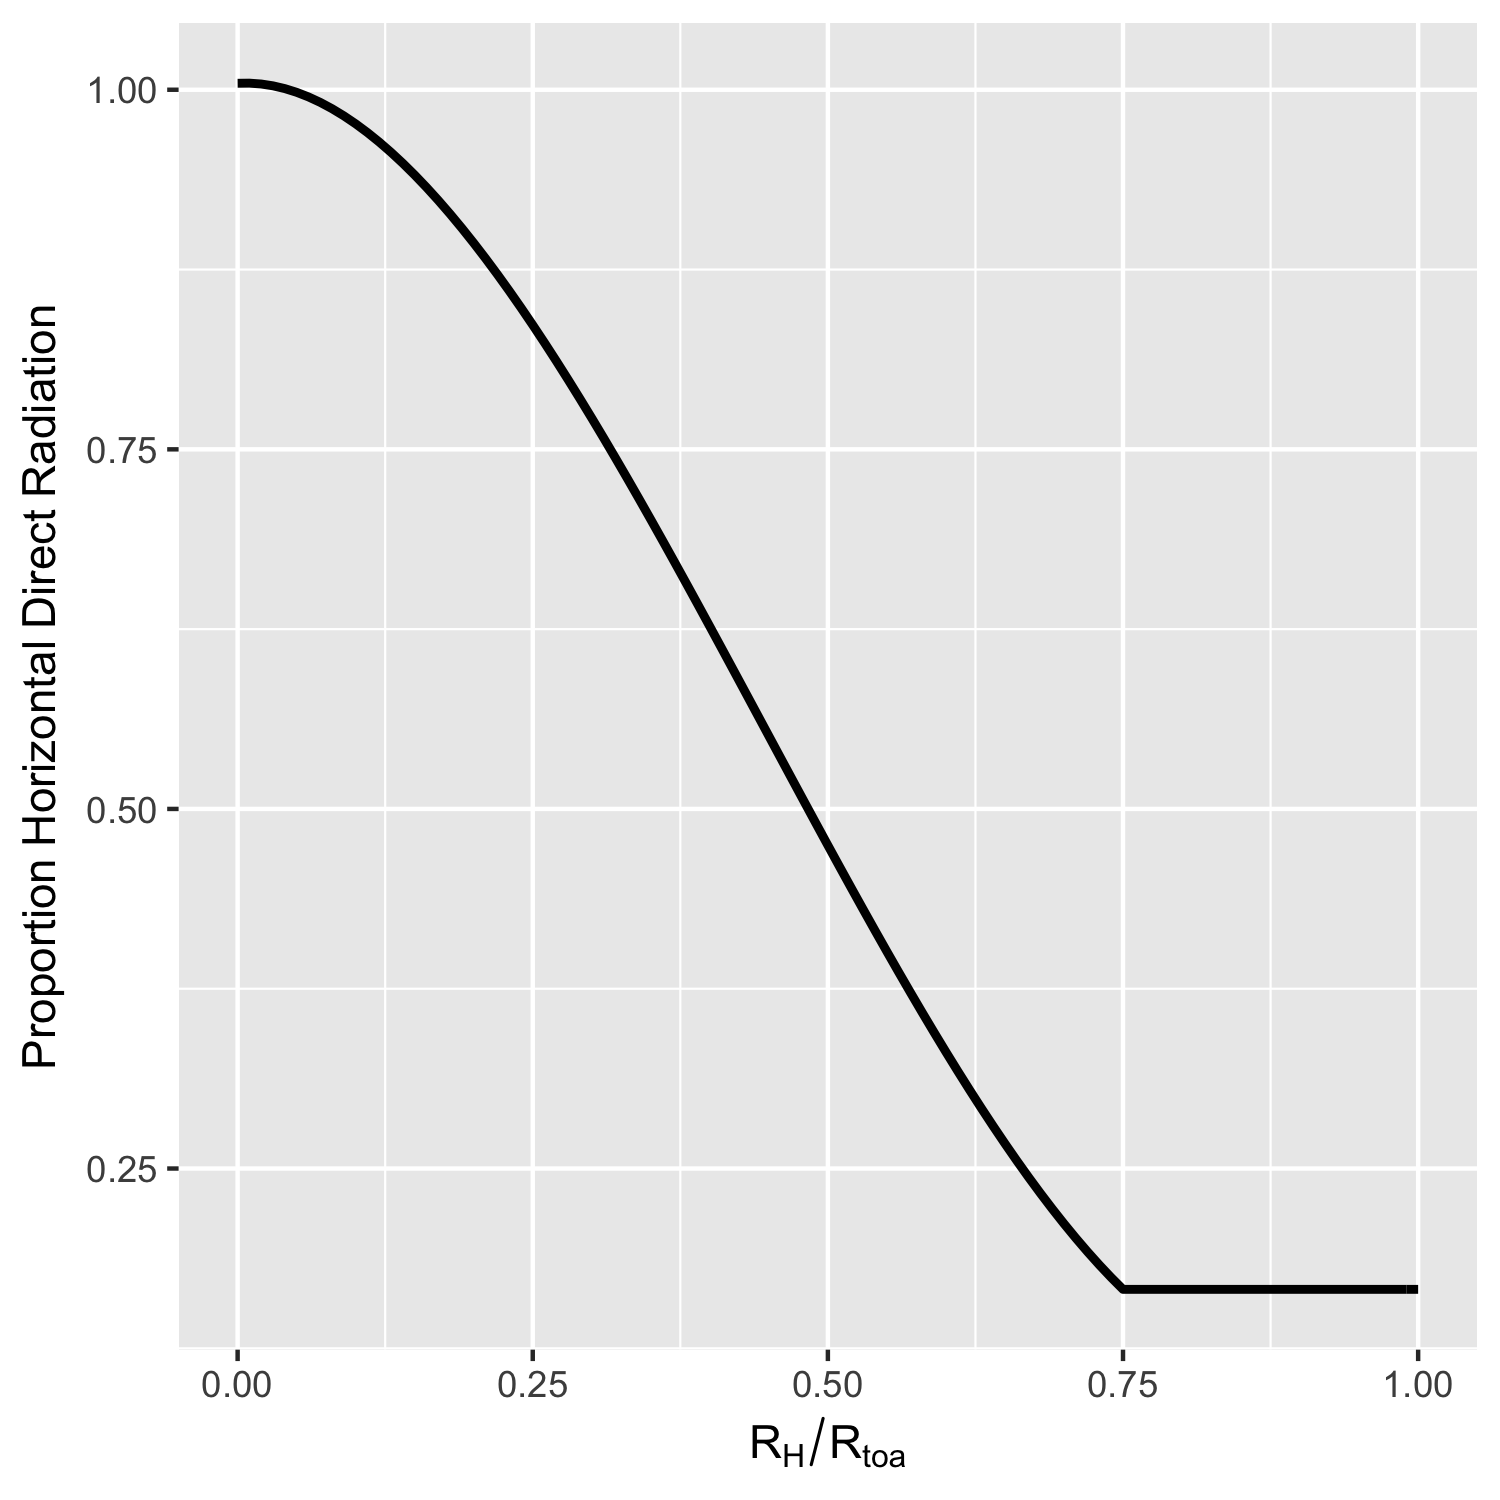
\includegraphics[width=0.55\linewidth]{Figures/Keith_Kreider.png}
  \caption{Relationship of fraction of TOA radiation attenuated by the atmosphere to direct radiation on a horizontal surface \protect\cite{keithPrinciplesSolarEngineering1978} (Eq. \ref{kk}).}
  \label{fig:KK}
\end{figure}

where $K_t$ is the fraction of top-of-atmosphere solar radiation attenuated by the atmosphere ($K_t = \frac{R_H}{R_{toa}}$). Horizontal direct beam radiation ($R_{Hb}$, cal cm$^{-2}$ day$^{-1}$) is then calculated as:

\begin{equation}
R_{Hb} = R_H - R_{Hd}
\end{equation}

Tilt factors, calculated using a site's slope and aspect, are used to convert horizontal surface diffuse and direct radiation into actual diffuse and direct radiation using equations from \citeA{bonanComputerModelSolar1989} and \citeA{liuDailyInsoluationSurfaces1962}. The direct beam tilt factor is calculated using the daily sums of the cosine of hourly solar incidence angles and sine of hourly solar altitude angles. 

\begin{figure}
  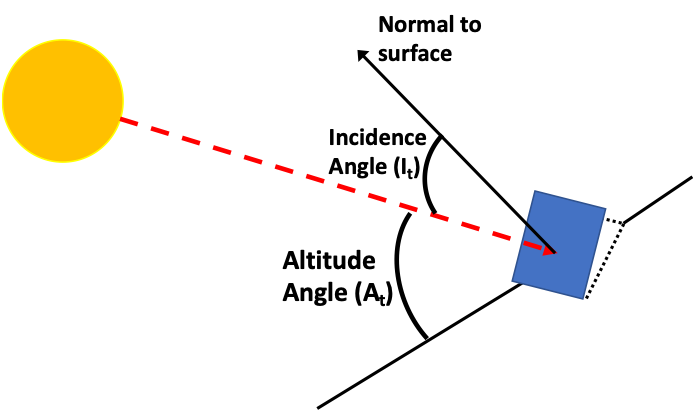
\includegraphics[width=0.6\linewidth]{Figures/Azimuth_Incidence.png}
  \caption{Solar altitude and incidence angles for a tilted surface.}
  \label{fig:aziinc}
\end{figure}

For each day in the simulation, hourly solar altitude angles ($A_t$, radians) (i.e. altitude of the Sun relative to the Earth's horizon; Fig. \ref{fig:aziinc}) depend on latitude ($\phi$, radians), solar declination ($\delta$, radians), and the solar hour angle: 

\begin{equation}
A_t = \arcsin{\Big(\sin{(\phi)}\sin{(\delta)} + \cos{(\phi)}\cos{(\delta)}\cos{(h_s)}\Big)}
\end{equation}

where $h_s$ is the solar hour angle (radians), calculated as $h_s = 15(12 - \frac{2t - 1}{2})(\frac{\pi}{180})$, where $t$ is hours from midnight. Hourly solar incidence angles ($I_t$, radians) (i.e. the angle at which the Sun's rays strike a surface; Fig. \ref{fig:aziinc}) are calculated using latitude, solar declination, solar hour angle, and surface orientation:

\begin{equation}
  \begin{split}
    I_t = \arccos\Big( & \sin{(\delta)}\sin{(\phi)}\cos{(z)} - \\
    & \sin{(\delta)}\cos{(\phi)}\sin{(z)}\cos{(a_z)} +  \\
     &  \cos{(\delta)}\cos{(h_s)}\cos{(\phi)}\cos{(z)} + \\
     & \cos{(\delta)}\cos{(h_s)}\sin{(\phi)}\sin{(z)}\cos{(a_z)} + \\
     & \cos{(\delta)}\sin{(z)}\sin{(a_z)}\sin{(h_s)}\Big)
  \end{split}
\end{equation}

where $z$ is the slope of the site (radians) and $a_z$ is the wall azimuth angle (radians), calculated as $a_z = (180-a)(\frac{\pi}{180})$, where $a$ is the site's aspect (degrees) (Fig. \ref{fig:angles}).

\begin{figure}
  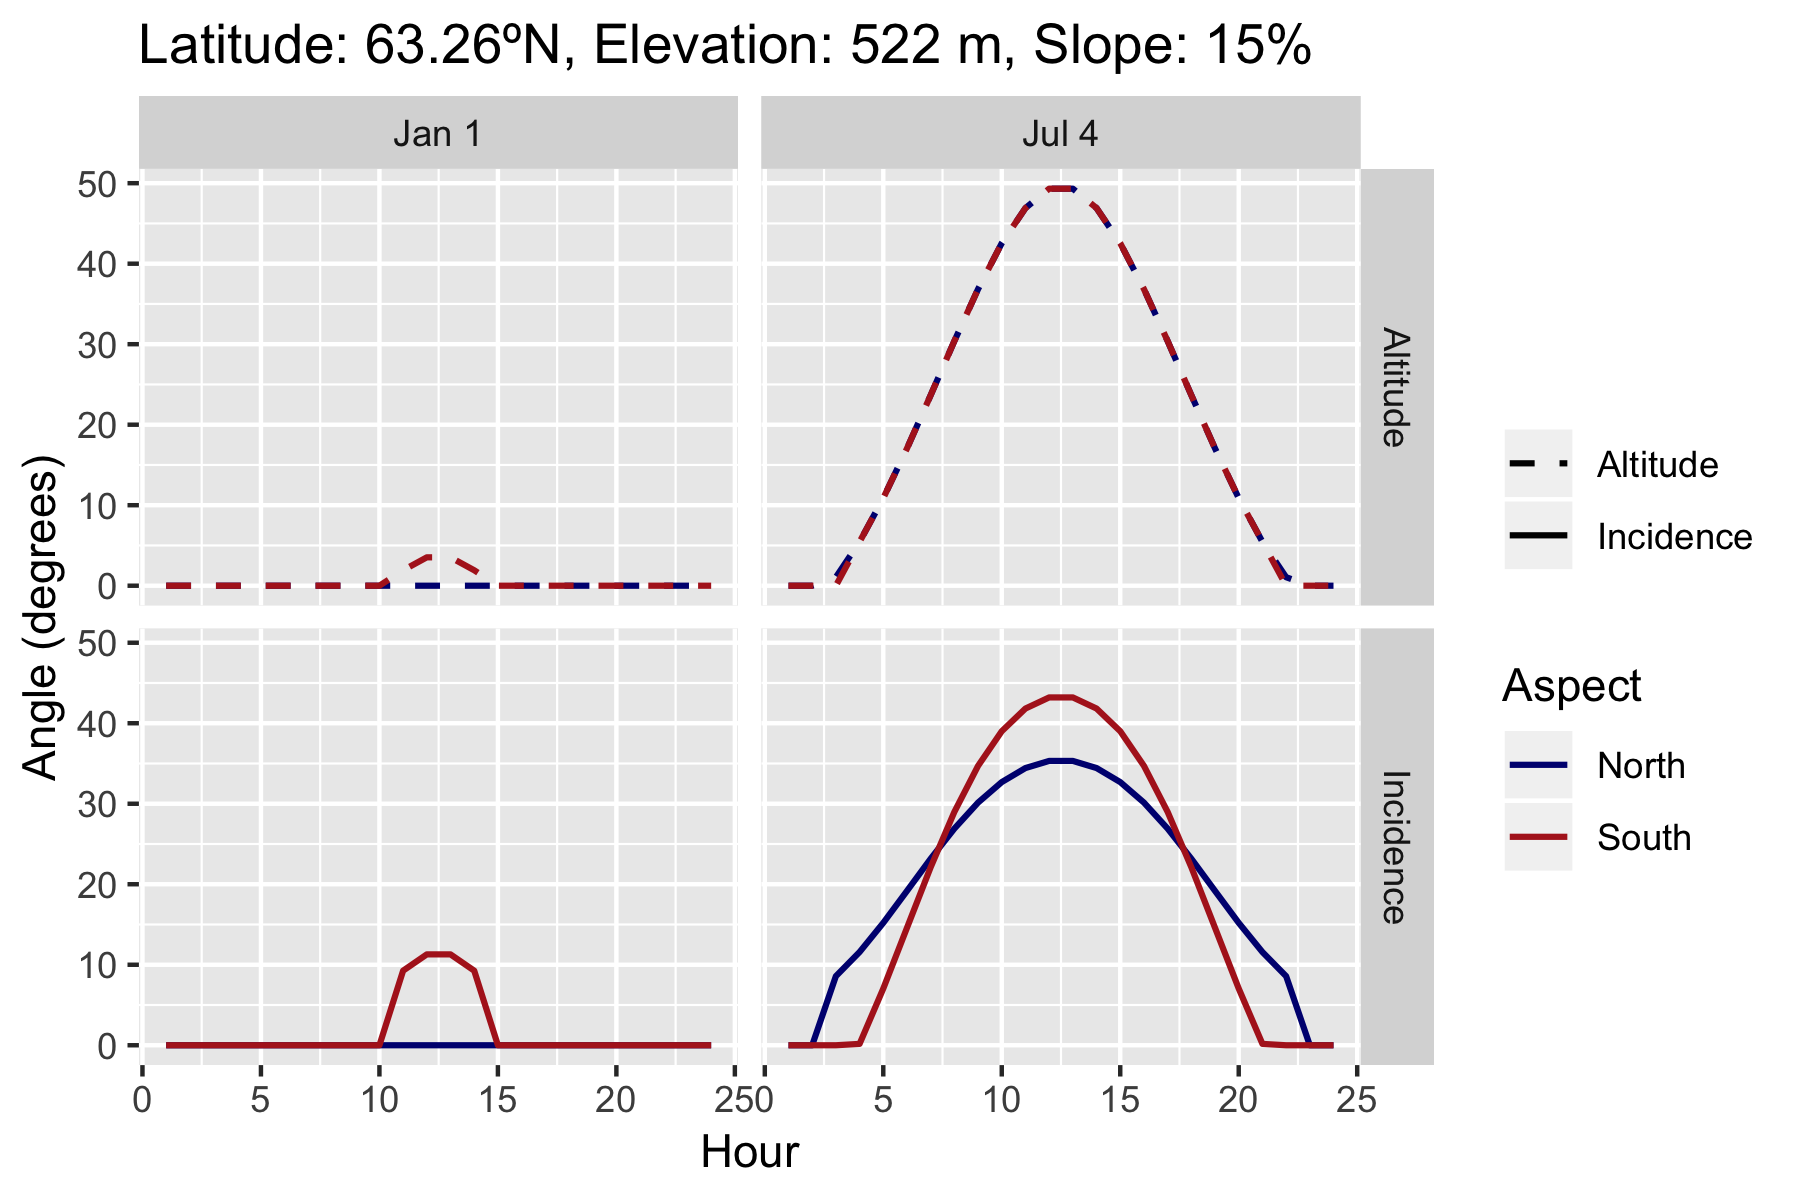
\includegraphics[width=0.8\linewidth]{Figures/Solar_Angles.png}
  \caption{Calculation of hourly incidence and altitude angles for two days at north- and south-facing slopes in interior Alaska.}
  \label{fig:angles}
\end{figure}

The cosine of hourly incidence and sine of hourly altitude angles are summed for each day to derive daily sums of altitude and incidence angles. It is assumed that the Sun is not above the horizon or in front of the surface when $A_t \le 0$º or when $I_t \ge 90$º. At these times, the angles are not added to the daily sums.

The direct beam tilt factor ($F_b$) is then calculated as:

\begin{equation}
F_b = \frac{I_{sum}}{A_{sum}}
\end{equation}

where $I_{sum}$ is the incidence angle sum, and $A_{sum}$ is the altitude angle sum (radians). The diffuse radiation tilt factor ($F_d$) is calculated as:

\begin{equation}
F_d = \Big(\cos(\frac{z}{2})\Big)^2
\end{equation}

These tilt factors are used to calculate the diffuse, direct, and total solar radiation received at the surface (cal cm$^{-2}$ day$^{-1}$):

\begin{equation}
R = F_bR_{Hb} + F_dR_{Hd}
\end{equation}

In this way, south-facing and north-facing slopes at the same latitude will receive different amounts of solar radiation throughout the year (Fig. \ref{fig:finalrad}), impacting the amount of PET and thus the site's moisture dynamics.

\begin{figure}
  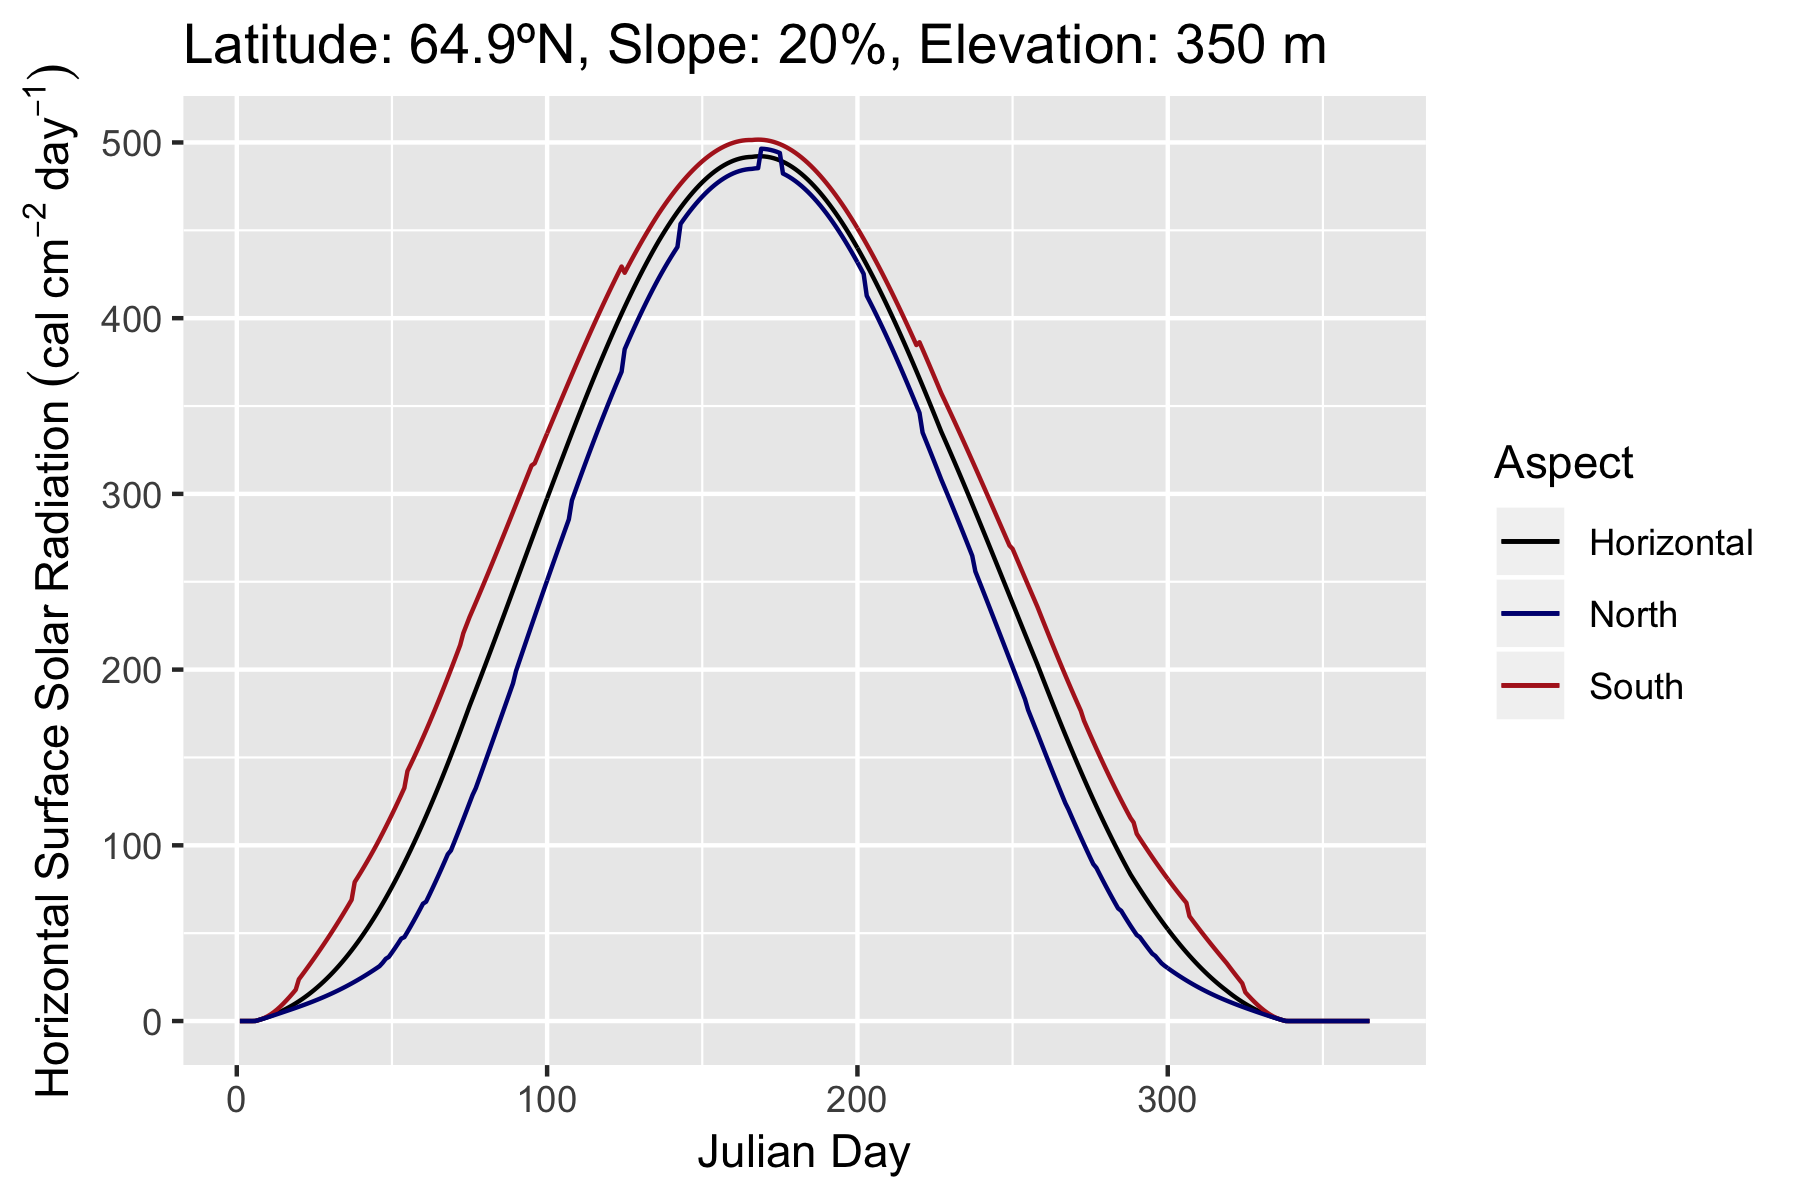
\includegraphics[width=0.8\linewidth]{Figures/Final_Radiation.png}
  \caption{Example simulation of daily surface solar radiation (cal cm$^{-2}$ day$^{-1}$) for a location in interior Alaska with no slope and with 20\% north- and south-facing slopes.}
  \label{fig:finalrad}
\end{figure}

\subsection{Potential Evapotranspiration} \label{pet}
In previous versions of UVAFME, top-of-atmosphere radiation was used to calculate potential evapotranspiration (PET) using Hargreave's evaporation formula \cite{fosterValidationApplicationForest2017}, however, studies have shown this equation to overestimate PET at high latitudes \shortcite{rosenbergMicroclimate1983, bonanComputerModelSolar1989}. In Version 3 of the model, the formulation for PET was updated to use a modified Priestley-Taylor equation as in \citeA{bonanComputerModelSolar1989}, which uses surface solar radiation, allowing for the incorporation of topographic effects on PET \cite{campbellIntroductionEnvironmentalBiophysics1977}:

\begin{equation}
PET=\begin{cases}
	\frac{a(t_{av} - b)R}{h_{vap}}, & \text{$t_{av} > 0$}.\\
	0 & \text{$t_{av} \leq 0$}.
  \end{cases}
\end{equation}

where $t_{av}$ is the mean daily temperature (ºC), $h_{vap}$ is the latent heat of vaporization (kcal kg$^{-1}$), calculated as $h_{vap} = 597.391 - 0.5680t_{av}$, and $a$ and $b$ are site-specific coefficients, calculated using the average minimum and maximum daily temperatures of the warmest month of the year \cite{bosenFormulaApproximationSaturation1960}:

\begin{equation}
a = \frac{1}{38 - \frac{2E}{305} + \frac{380}{e_2 - e_1}}
\end{equation}

\begin{equation}
b = -2.5 - 0.14(e_2 - e_1) - \frac{E}{550}
\end{equation}

where $E$ is the site's elevation (m), and $e_1$ and $e_2$ are the saturation vapor pressures (mbar) at the mean minimum and maximum daily temperatures ($t_m$), respectively, of the warmest month of the year, calculated as:

\begin{equation}
e = 33.8639\Big((0.00738t_m + 0.8072)^8 - 0.000019|1.8t_m + 48| + 0.001316\Big)
\end{equation}

Using this updated formulation, PET can differ between cold north-facing sites and warm south-facing sites (Fig. \ref{fig:pet}), impacting soil moisture and plant growth.

\begin{figure}
  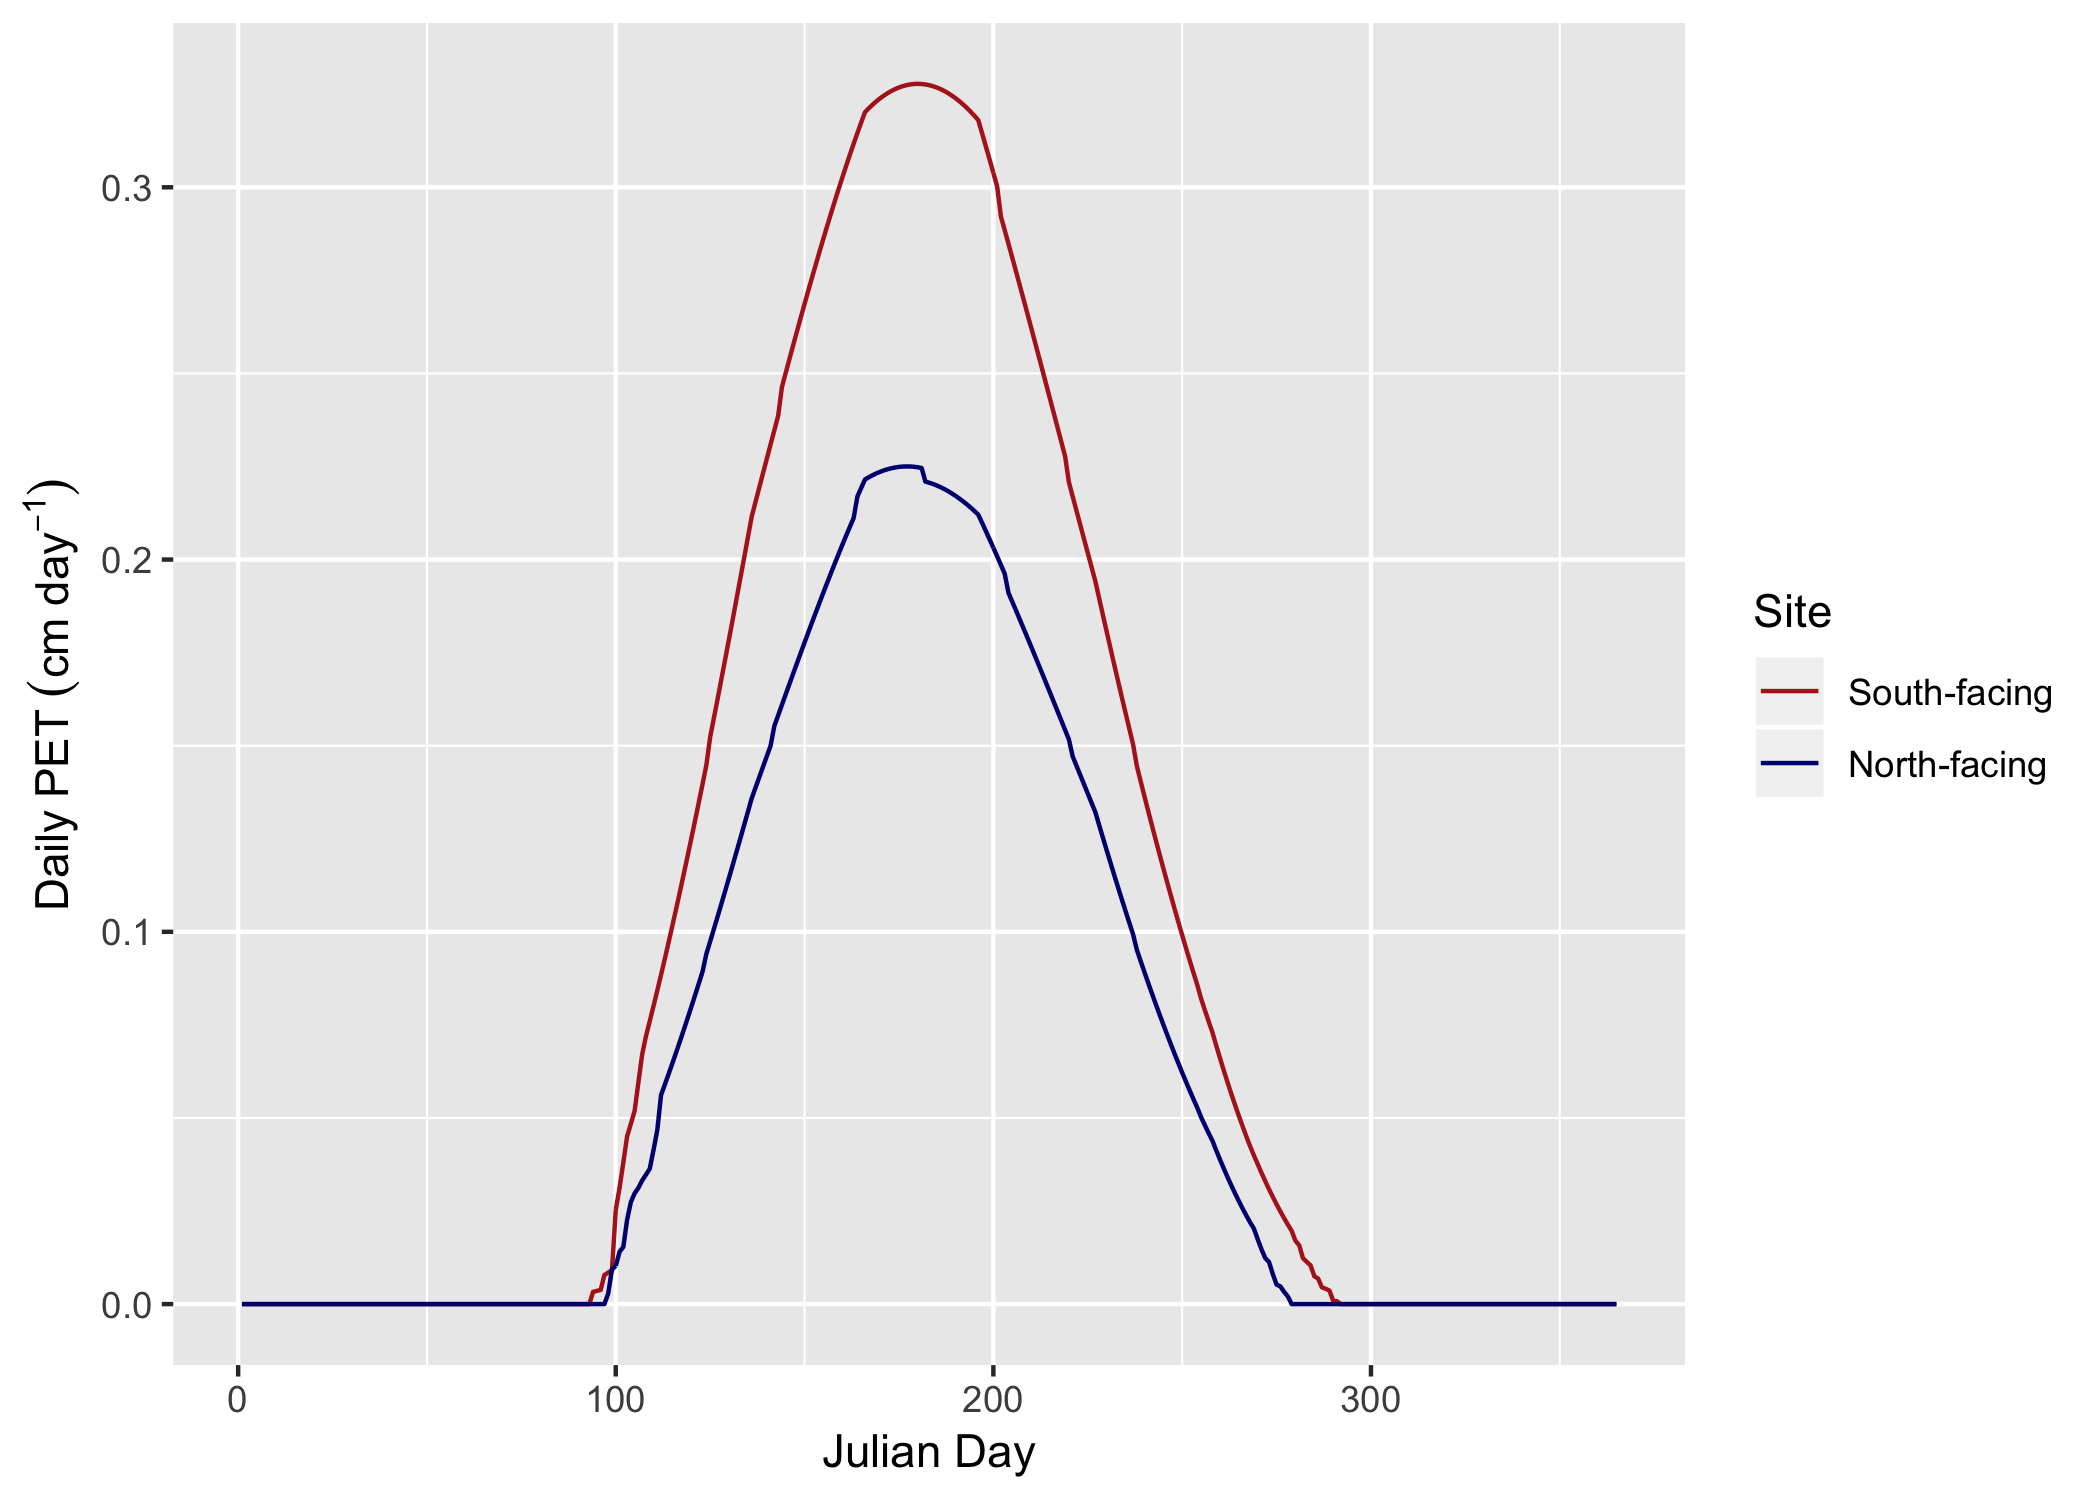
\includegraphics[width=0.85\linewidth]{Figures/PET.png}
  \caption{Example simulation of daily PET (cm day$^{-1}$) for a warm south-facing and a cold north-facing site in interior Alaska.}
  \label{fig:pet}
\end{figure} 

\section{Soil Processes} \label{soil}
\numberwithin{equation}{section}

\subsection{Soil Water} \label{soilwater}

Soil water balance in UVAFME is partitioned into two layers, a moss-organic layer containing a mixture of moss, humus, and litter, and a mineral (A) layer. Outputs are aggregated over the year to influence yearly vegetation growth. Using this simple model allows for relatively little inputs: slope, canopy LAI, organic layer depth, drainage quality, soil texture, PET, and precipitation. These inputs are received from site input parameters, the plant canopy module (Section \ref{gmult}), the soil nutrient submodel (Section \ref{nutrients}), and the climate module (Section \ref{climate}). 

This updated version of UVAFME also allows for the incorporation of permafrost depth effects on soil moisture dynamics (Section \ref{perm}). Each day in the simulation, soil moisture is partitioned into liquid and frozen water in each soil layer, based on the calculation of depths of freezing and thawing in the permafrost submodel. As in \citeA{bonanComputerModelSolar1989}, for areas with continuous or discontinuous permafrost, it is assumed that the moss-organic and mineral layers are above field capacity at the beginning of each year (i.e. January 1, $jd$ = 1). This effect of near-saturated conditions on moisture dynamics is implemented via drainage condition variables, which are set up at the beginning of each simulation year, based on the previous' years maximum depth of thaw ($alt$, m):

\begin{equation}
z_{drain} = \frac{m_{sat}(1 - alt) + m_{fc}(alt - 0.32)}{1 - 0.32}
\end{equation}

where $m_{sat}$ and $m_{fc}$ are the saturation and field capacities of the soil layer (volumetric). These drainage parameters are corrected so that they are between the soil layer's field capacity and saturation capacity. The organic and mineral layer field capacity, saturation capacity, and wilting point for each site are set to default values as in \citeA{bonanComputerModelSolar1989}, based on the site's drainage class (i.e. well-, moderately, or poorly drained) (Table \ref{tab:soiltable}).

\begin{table}
  \begin{center}
    \caption{Input soil parameters (volumetric). Values taken from \protect\citeA{bonanComputerModelSolar1989}.}
    \label{tab:soiltable}
     \resizebox{\textwidth}{!}{\begin{tabular}{c|c|c|c|c} 
      \textbf{Soil Layer} & \textbf{Variable} & \textbf{Well drained} & \textbf{Moderately drained} & \textbf{Poorly drained}\\
      \hline
      \multirow{3}{*}{organic} & saturation capacity & 0.39 & 0.39 & 0.39\\
      & field capacity & 0.39 & 0.39 & 0.39\\
      & permanent wilting point & 0.039 & 0.039 & 0.039\\
      \hline
      \multirow{3}{*}{\begin{tabular}{c}mineral\\
(A-layer)
\end{tabular}} & saturation capacity & 0.35 & 0.44 & 0.53\\
      & field capacity & 0.20 & 0.29 & 0.38\\
      & permanent wilting point & 0.06 & 0.06 & 0.06\\
    \end{tabular}}
  \end{center}
\end{table}

This drainage variable ($z_{drain}$) is used to modify the actual field and saturation capacities of soil (see below) and to calculate each soil layer's gravimetric moisture content at the beginning of the year as $gw = \frac{\rho_{water}z_{drain}}{bd_s}$, where $bd_s$ is the soil layer's bulk density, set to 85 kg m$^{-3}$ for the organic layer and 1250 kg m$^{-3}$ for the mineral layer \cite{bonanComputerModelSolar1989}. Additionally,  it is assumed that all soil moisture at the beginning of the year is frozen (i.e. $w_i = z_{drain}d_s$ and $w_l = 0.0$, where $w_i$ and $w_l$ are the amounts of frozen and liquid water, respectively in the soil layer (m), and $d_s$ is the depth of the soil layer (m)).

\subsubsection{Soil Moisture Dynamics}

The amount of soil moisture (liquid and frozen) is updated on a daily time step, incorporating effects from precipitation, canopy interception, runoff, snowpack melt, soil freezing and thawing, soil water infiltration, and evaporation (Fig. \ref{fig:soildiagram}).

\begin{figure}
  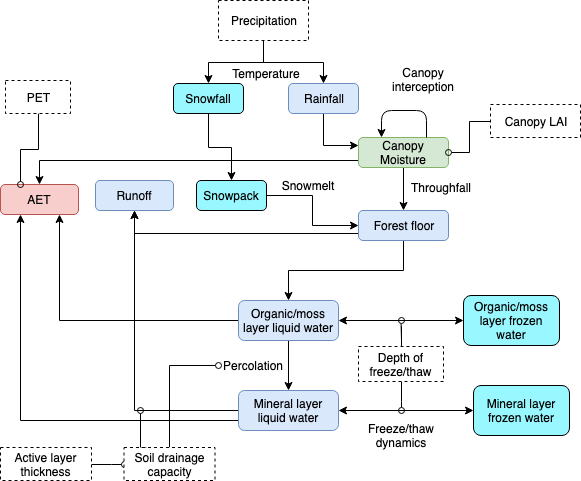
\includegraphics[width=0.8\linewidth]{Figures/SoilMoisture.png}
  \caption{Flow diagram showing moisture dynamics simulated in UVAFME.}
  \label{fig:soildiagram}
\end{figure} 

 Precipitation (input from the climate module) is initially received at the surface. As in previous versions of UVAFME, precipitation is partitioned into liquid rainfall and snow, depending on temperature. In this updated version, a new equation was used for simulating a mixture of snow and rain when the air temperature is near freezing. If the mean daily temperature is greater than or equal to 3.3ºC, all precipitation is assumed to be liquid rainfall. If $t_{av}$ is at or below -1.1ºC, all precipitation is assumed to be snow. If $t_{av}$ is between 3.3ºC and -1.1ºC, precipitation is assumed to be a mixture of snow and liquid water, with the portion  that falls as snow calculated as \shortcite{wigmostaDistributedHydrologyvegetationModel1994}:

\begin{equation}
P_{snow} = \frac{(3.3 - t_{av})}{(3.3 - -1.1)}P 
\end{equation}

where $P$ is total precipitation (m) and $P_{snow}$ is snowfall in snow-water-equivalent (m). All snowfall is then accumulated in an annual snowpack and snow-water equivalent (SWE) bank. Canopy interception ($I$, m) from liquid rainfall is calculated as:

\begin{equation}
I = \min\Big(\max(laiw_{max} - laiw, 0.0), P_{rain}\Big)
\end{equation}

where $laiw_{max}$ is the maximum water content of the canopy (m), calculated as $0.0015LAI$, and $laiw$ is the current water content of the canopy (m). Throughfall is then calculated as $t_{fall} = \max(P_{rain} - I, 0.0)$, and the water content of the canopy is increased by the interception amount.

When there is snow on the ground and the air temperature is above freezing, the snowpack melt amount (m) is calculated using the degree method \shortcite{singhDegreedayFactorsSnow2000}:

\begin{equation}
s_{melt} = 0.001\Big(c_m(t_{av} - t_c)\Big)
\end{equation}

where $c_m$ is a site-specific coefficient, set to 4.0 for forested sites \shortcite{dewalleSpatialTemporalVariations2002}, and $t_c$ is the critical freezing temperature, set to 0.0ºC. The snow-water equivalent bank is then decreased by the snowmelt amount, and the snowpack depth is updated as:

\begin{equation}
d_{snow} = \frac{swe}{\frac{\rho_{snow}}{\rho_w}}
\end{equation}

where $swe$ is snow-water equivalent (m), $\rho_{snow}$ is the density of snow, set to 217 kg m$^{-3}$ \cite{sturmEstimatingSnowWater2010}, and $\rho_w$ is the density of water (1000 kg m$^{-3}$) (Fig. \ref{fig:snow}). 

\begin{figure}
  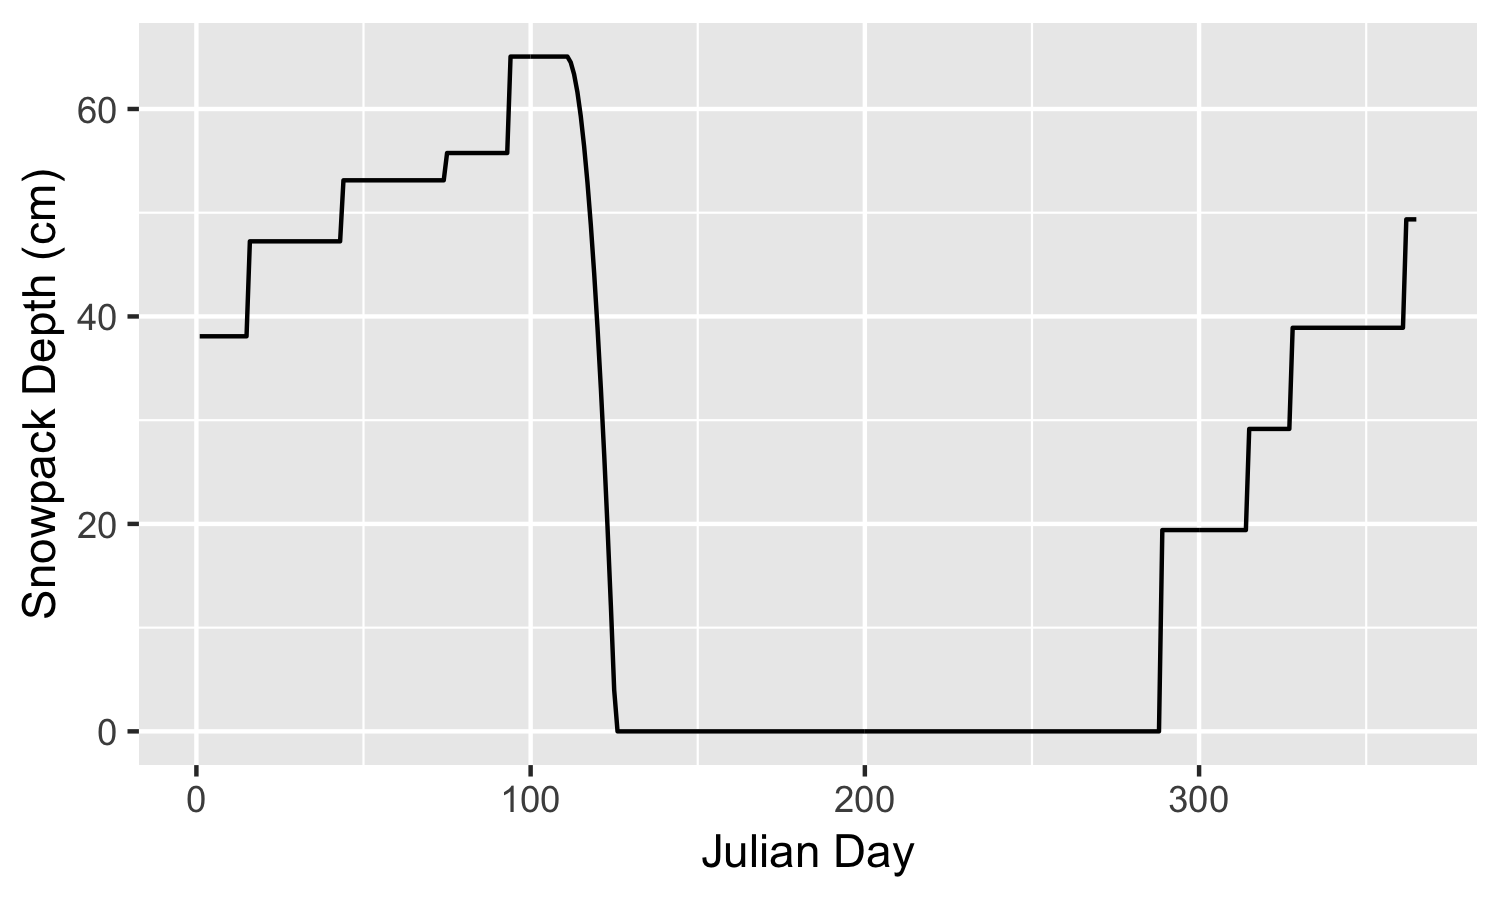
\includegraphics[width=0.8\linewidth]{Figures/SnowPack.png}
  \caption{Example simulation of snowpack accumulation and melt (cm day$^{-1}$) for a site in interior Alaska.}
  \label{fig:snow}
\end{figure} 

Slope runoff is then calculated as:

\begin{equation} \label{slr}
R_s = \Big({\frac{\theta}{90}}\Big)^2t_{fall}
\end{equation}

where $\theta$ is the slope of the site (degrees). Potential water loss or gain for the simulation day is calculated as:

\begin{equation} \label{pwl}
pw = t_{fall} + s_{melt} - R_s - PET
\end{equation}

In this updated version of UVAFME, the amount of water that freezes and thaws each day is also calculated based on \citeA{bonanComputerModelSolar1989} and incorporated into the soil moisture dynamics. For each soil layer (i.e. the moss-organic and mineral layers), the amount of water released in soil thawing ($w_t$, m) is calculated as a proportion of the change in depth of thaw from the previous day to the current simulation day:

\begin{equation}
w_t= \min\Big(z_{drain}(d_{thaw} - d'_{thaw}), w_i\Big)
\end{equation}

where $d_{thaw}$ is the depth of thaw in that layer (see Section {\ref{perm}}) on the current day (m), $d'_{thaw}$ is the depth of thaw from the previous day (m), and $w_i$ is the ice content of that layer (m). This amount is subtracted from the ice water content of the soil layer and added to the liquid water content. The depth of thaw is also used to update that layer's saturation capacity, field capacity, and wilting point:

\begin{equation} \label{ms}
m'_{sat} = m_{sat}d_{thaw}
\end{equation}

\begin{equation} \label{mfc}
m'_{fc} = m_{fc}d_{thaw}
\end{equation}

\begin{equation} \label{mpw}
m'_{pwp} = m_{pwp}d_{thaw}
\end{equation}

After the soil thawing is accounted for, if there is a positive water balance from precipitation (i.e. $pw \ge 0.0$ from Eq. \ref{pwl}), actual evapotranspiration ($AET$, m) is set equal to PET, and the positive water balance is added to the organic-moss layer, adjusting for excess water from infiltration and thawing. Excess water ($w_{exs} = \max(w_l - m_{fc}, 0.0)$, in m) within a layer is removed using a modified equation from \citeA{botkinForestDynamicsEcological1993}. This formulation assumes that as rainfall/water input intensity increases or as the soil layer becomes more saturated, the amount of runoff/soil percolation increases (Fig. \ref{fig:exs}). The proportion of excess water that runs off or percolates to a lower layer is calculated as:

\begin{equation} \label{exseq}
f_{exs} = b\Big(\frac{{w_{exs}}^2}{PET + w_{exs}}\Big)\Big(1 - (m_{fc} - m_{pwp})\Big)
\end{equation}

where $b$ is based on soil texture and is set to 2.0 for coarse-grained soils and 0.6 for fine-grained soils. Excess water is then subtracted from the soil layer as:

\begin{equation} \label{wl}
w_l = w_l - w_{exs}f_{exs}
\end{equation}

\begin{figure}
  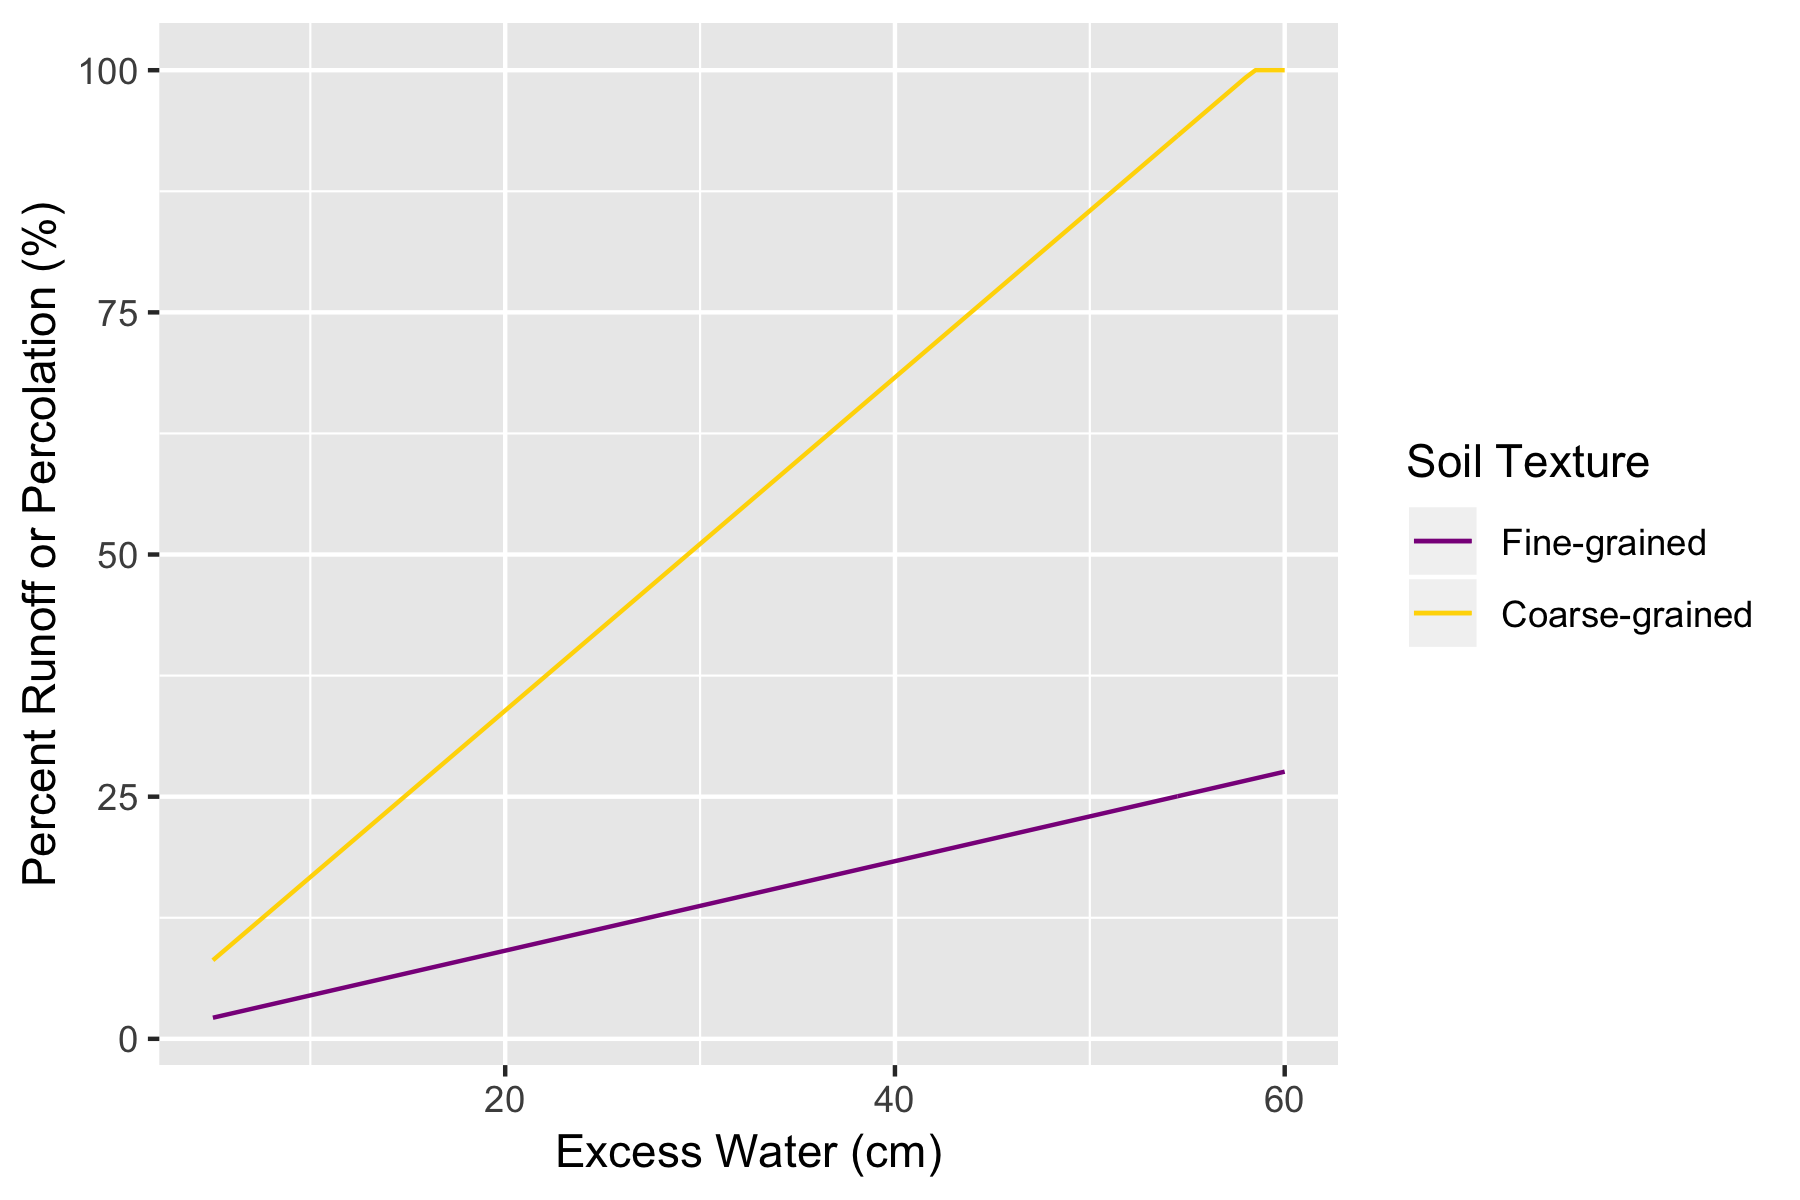
\includegraphics[width=0.8\linewidth]{Figures/Exs.png}
  \caption{Example calculation of fraction of excess water (above field capacity) that runs off or percolates to a lower soil layer for a coarse-grained and fine-grained soil with PET = 0.3 cm day$^{-1}$ (Eq. \ref{exseq}).}
  \label{fig:exs}
\end{figure} 

The excess water from the moss-organic layer is transferred to the mineral layer, and excess water from the mineral layer is calculated and subtracted (Fig. \ref{fig:liquid}, \ref{fig:liquidcumm}).

\begin{figure}
  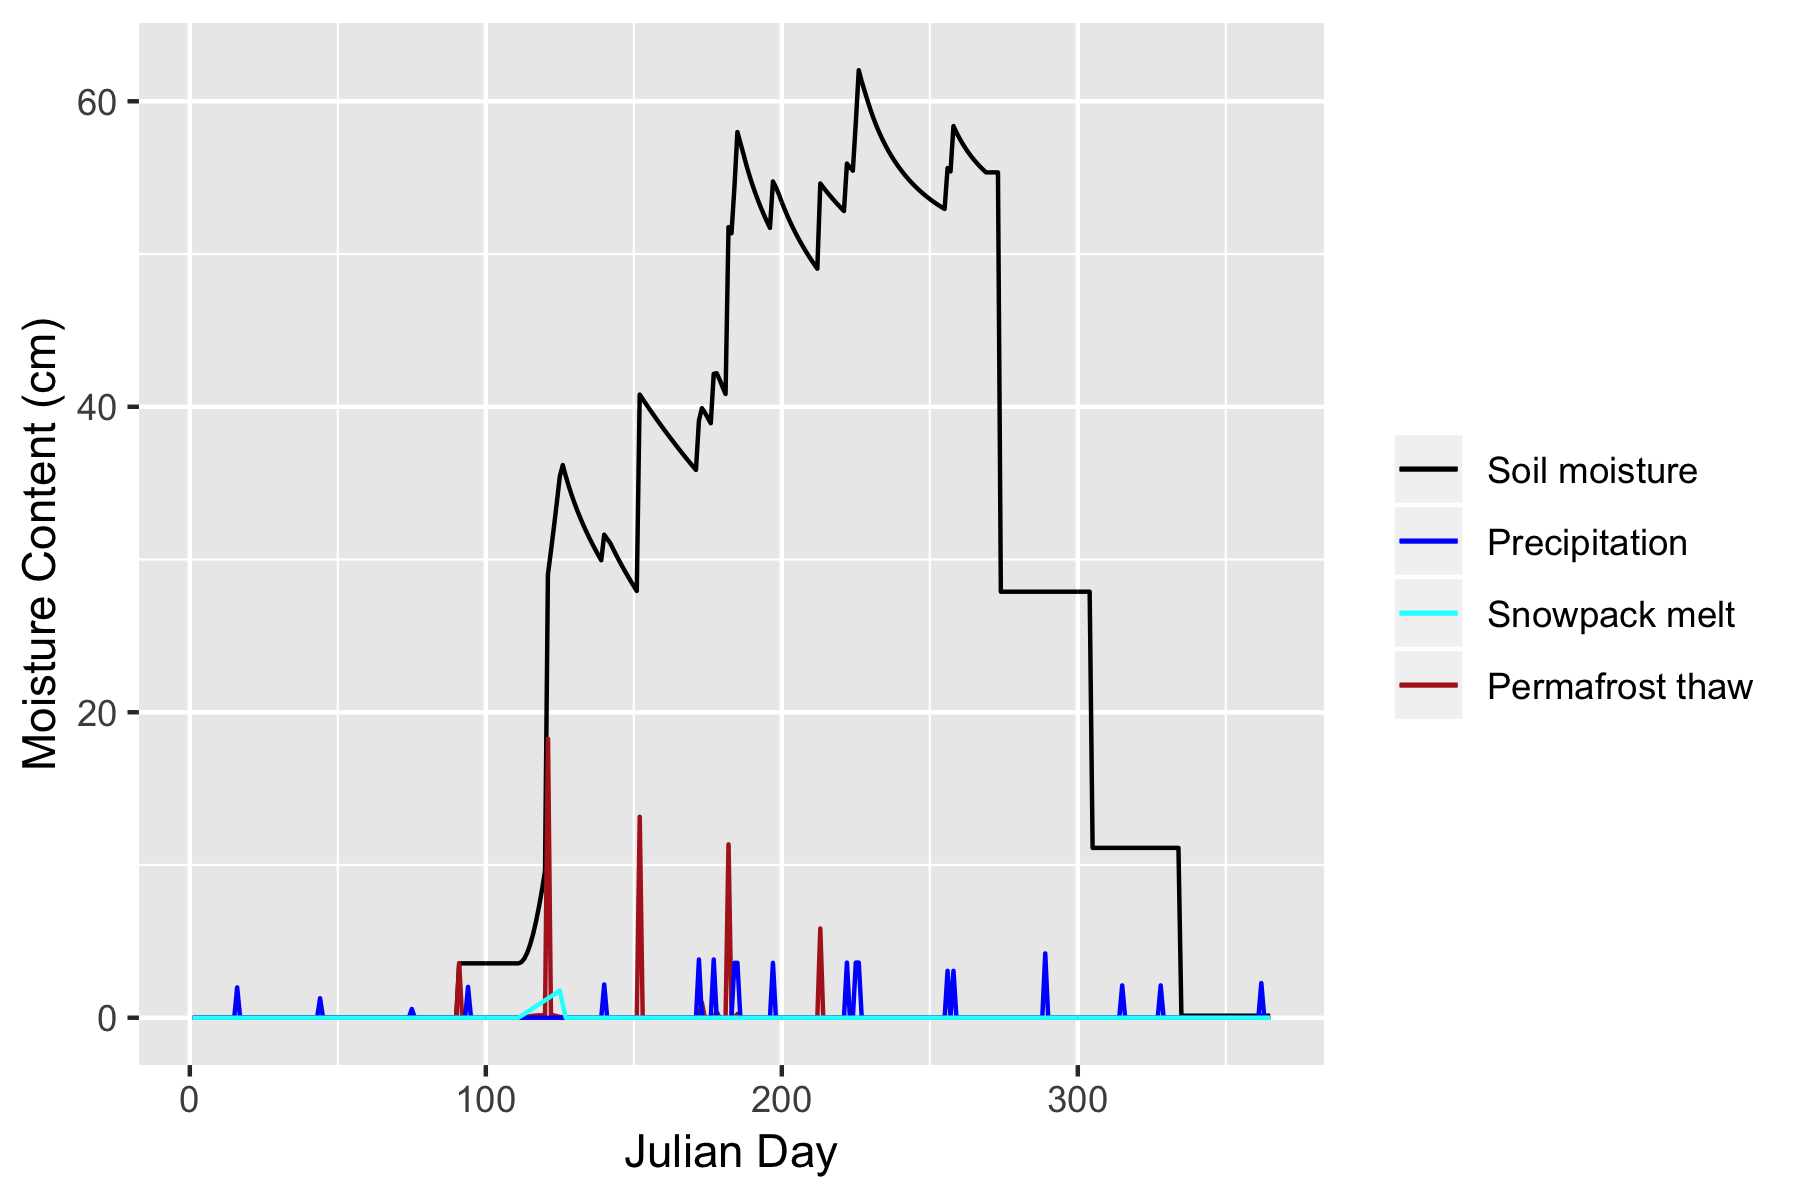
\includegraphics[width=0.8\linewidth]{Figures/Water.png}
  \caption{Example simulation of liquid soil moisture (cm) throughout the year for a site in interior Alaska. Dark blue lines indicate precipitation inputs, red lines indicate water from soil thawing, and cyan lines indicate water from snowpack melt.}
  \label{fig:liquid}
\end{figure}

\begin{figure}
  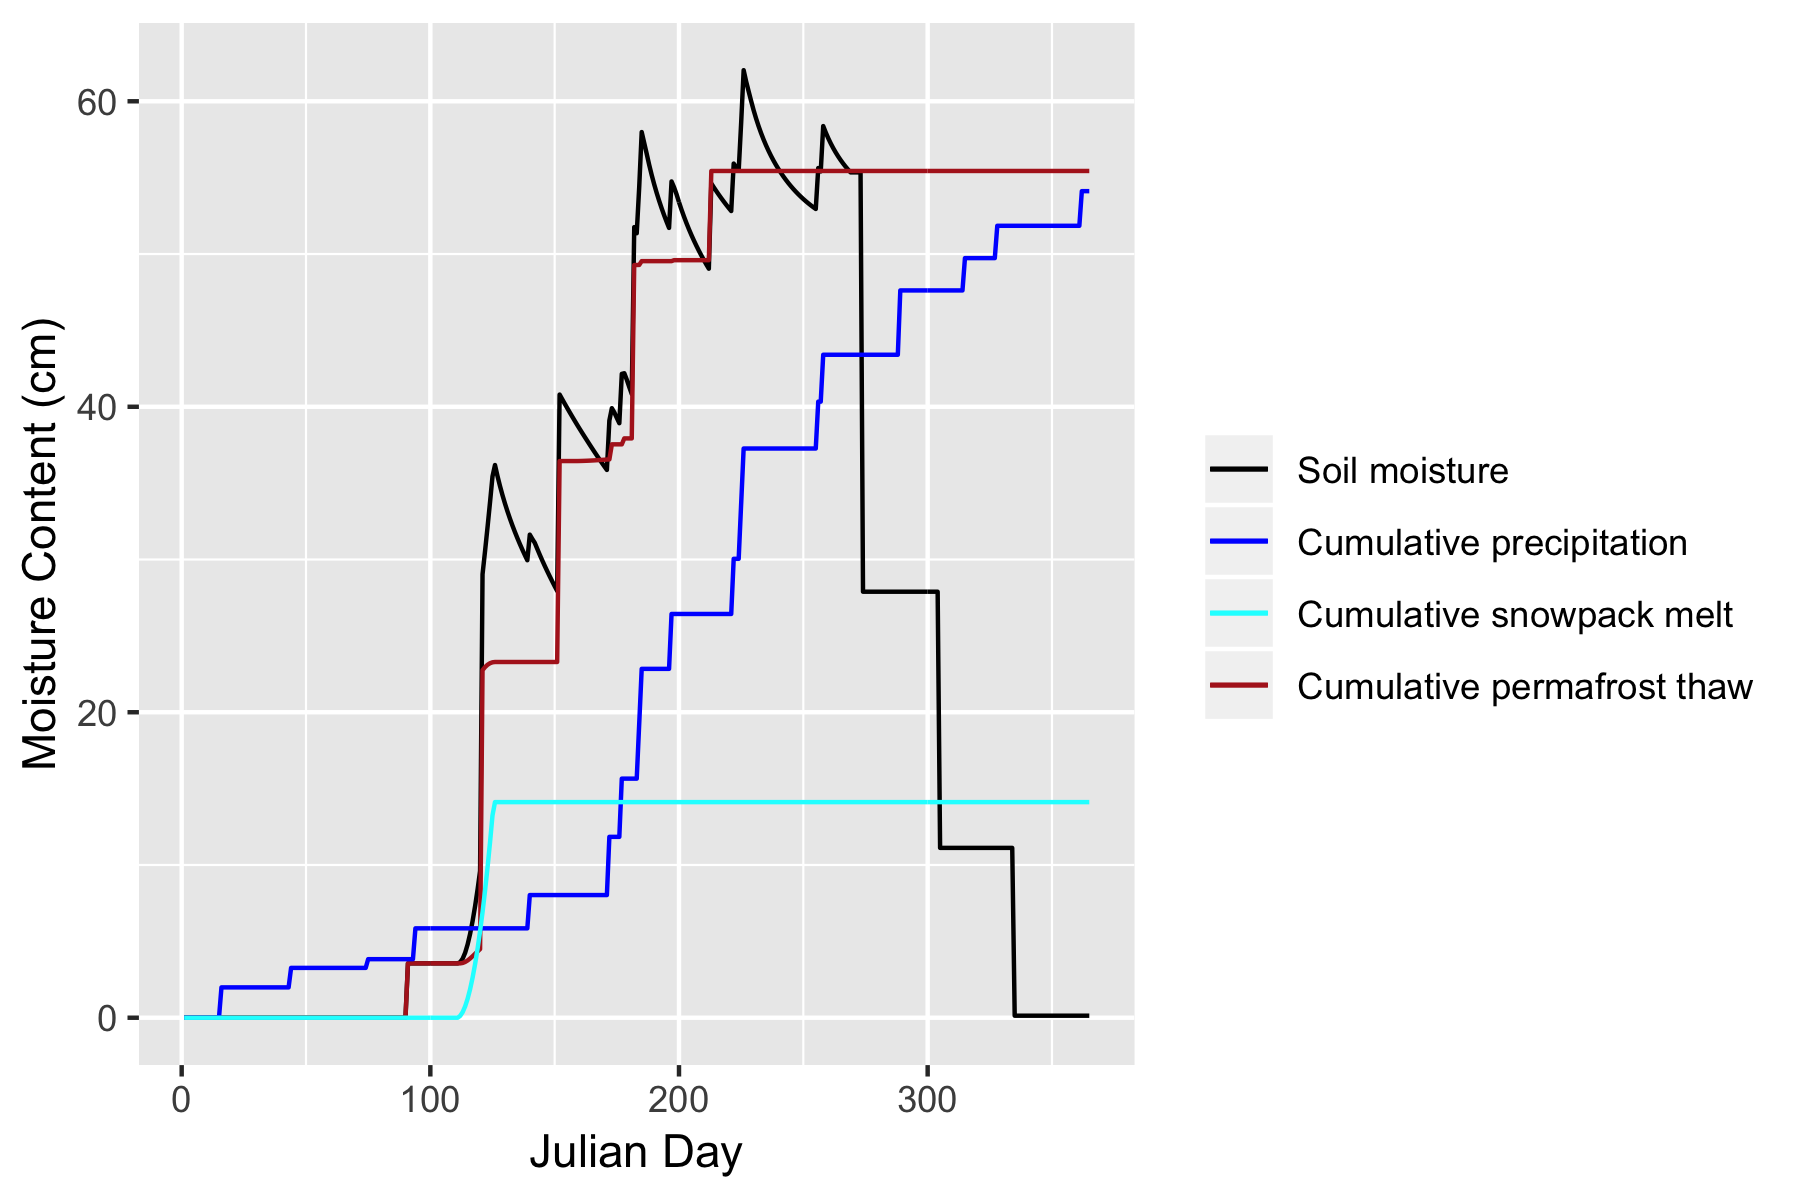
\includegraphics[width=0.8\linewidth]{Figures/Water_cumm.png}
  \caption{Example simulation of liquid soil moisture (cm) throughout the year for a site in interior Alaska. Dark blue lines indicate cumulative precipitation inputs, red lines indicate cumulative permafrost thaw, and cyan lines indicate cumulative snowpack melt.}
  \label{fig:liquidcumm}
\end{figure} 

If there is a negative water balance due to high PET or low moisture inputs (i.e. $pw < 0.0$, from Eq. \ref{pwl}), evaporation from the canopy and both soil layers occurs. Canopy evaporation ($E_{can}$, m) is calculated as:

\begin{equation}
E_{can} = \min\Big(-pw, \max(laiw - laiw_{min}, 0.0)\Big)
\end{equation}

where $laiw_{min}$ is the minimum water content of the canopy (m), calculated as $1.0\times10^{-4}LAI$. This evaporation amount is subtracted from the canopy water content, and $pw$ is increased (i.e. made less negative) to account for canopy evaporation:

\begin{equation}
pw = \min(pw + E_{can}, 0.0)
\end{equation}

If $pw$ is still negative, and there is at least some amount of unfrozen soil moisture (i.e. $d_{thaw} > 0.0$), evaporation occurs from the soil layers. The amount lost from each layer is dependent on the relative root distribution of each layer. As in \citeA{bonanComputerModelSolar1989}, the relative root distribution ($r_z$) for the organic layer is calculated as:

\begin{equation} \label{rooteq}
r_z =\Big( \frac{2d_{org}}{\min(d_{org} + alt, 1.0)}\Big)\Big(1 - \frac{d_{org}}{2(\min(d_{org} + alt, 1.0))}\Big)
\end{equation}

where $d_{org}$ is the depth of the organic layer (m) and $alt$ is the maximum depth of thaw from the previous year (m). Thus, with a deeper organic layer and a shallower active layer, more of the roots are distributed within the organic layer (Fig. \ref{fig:roots}).

\begin{figure}
  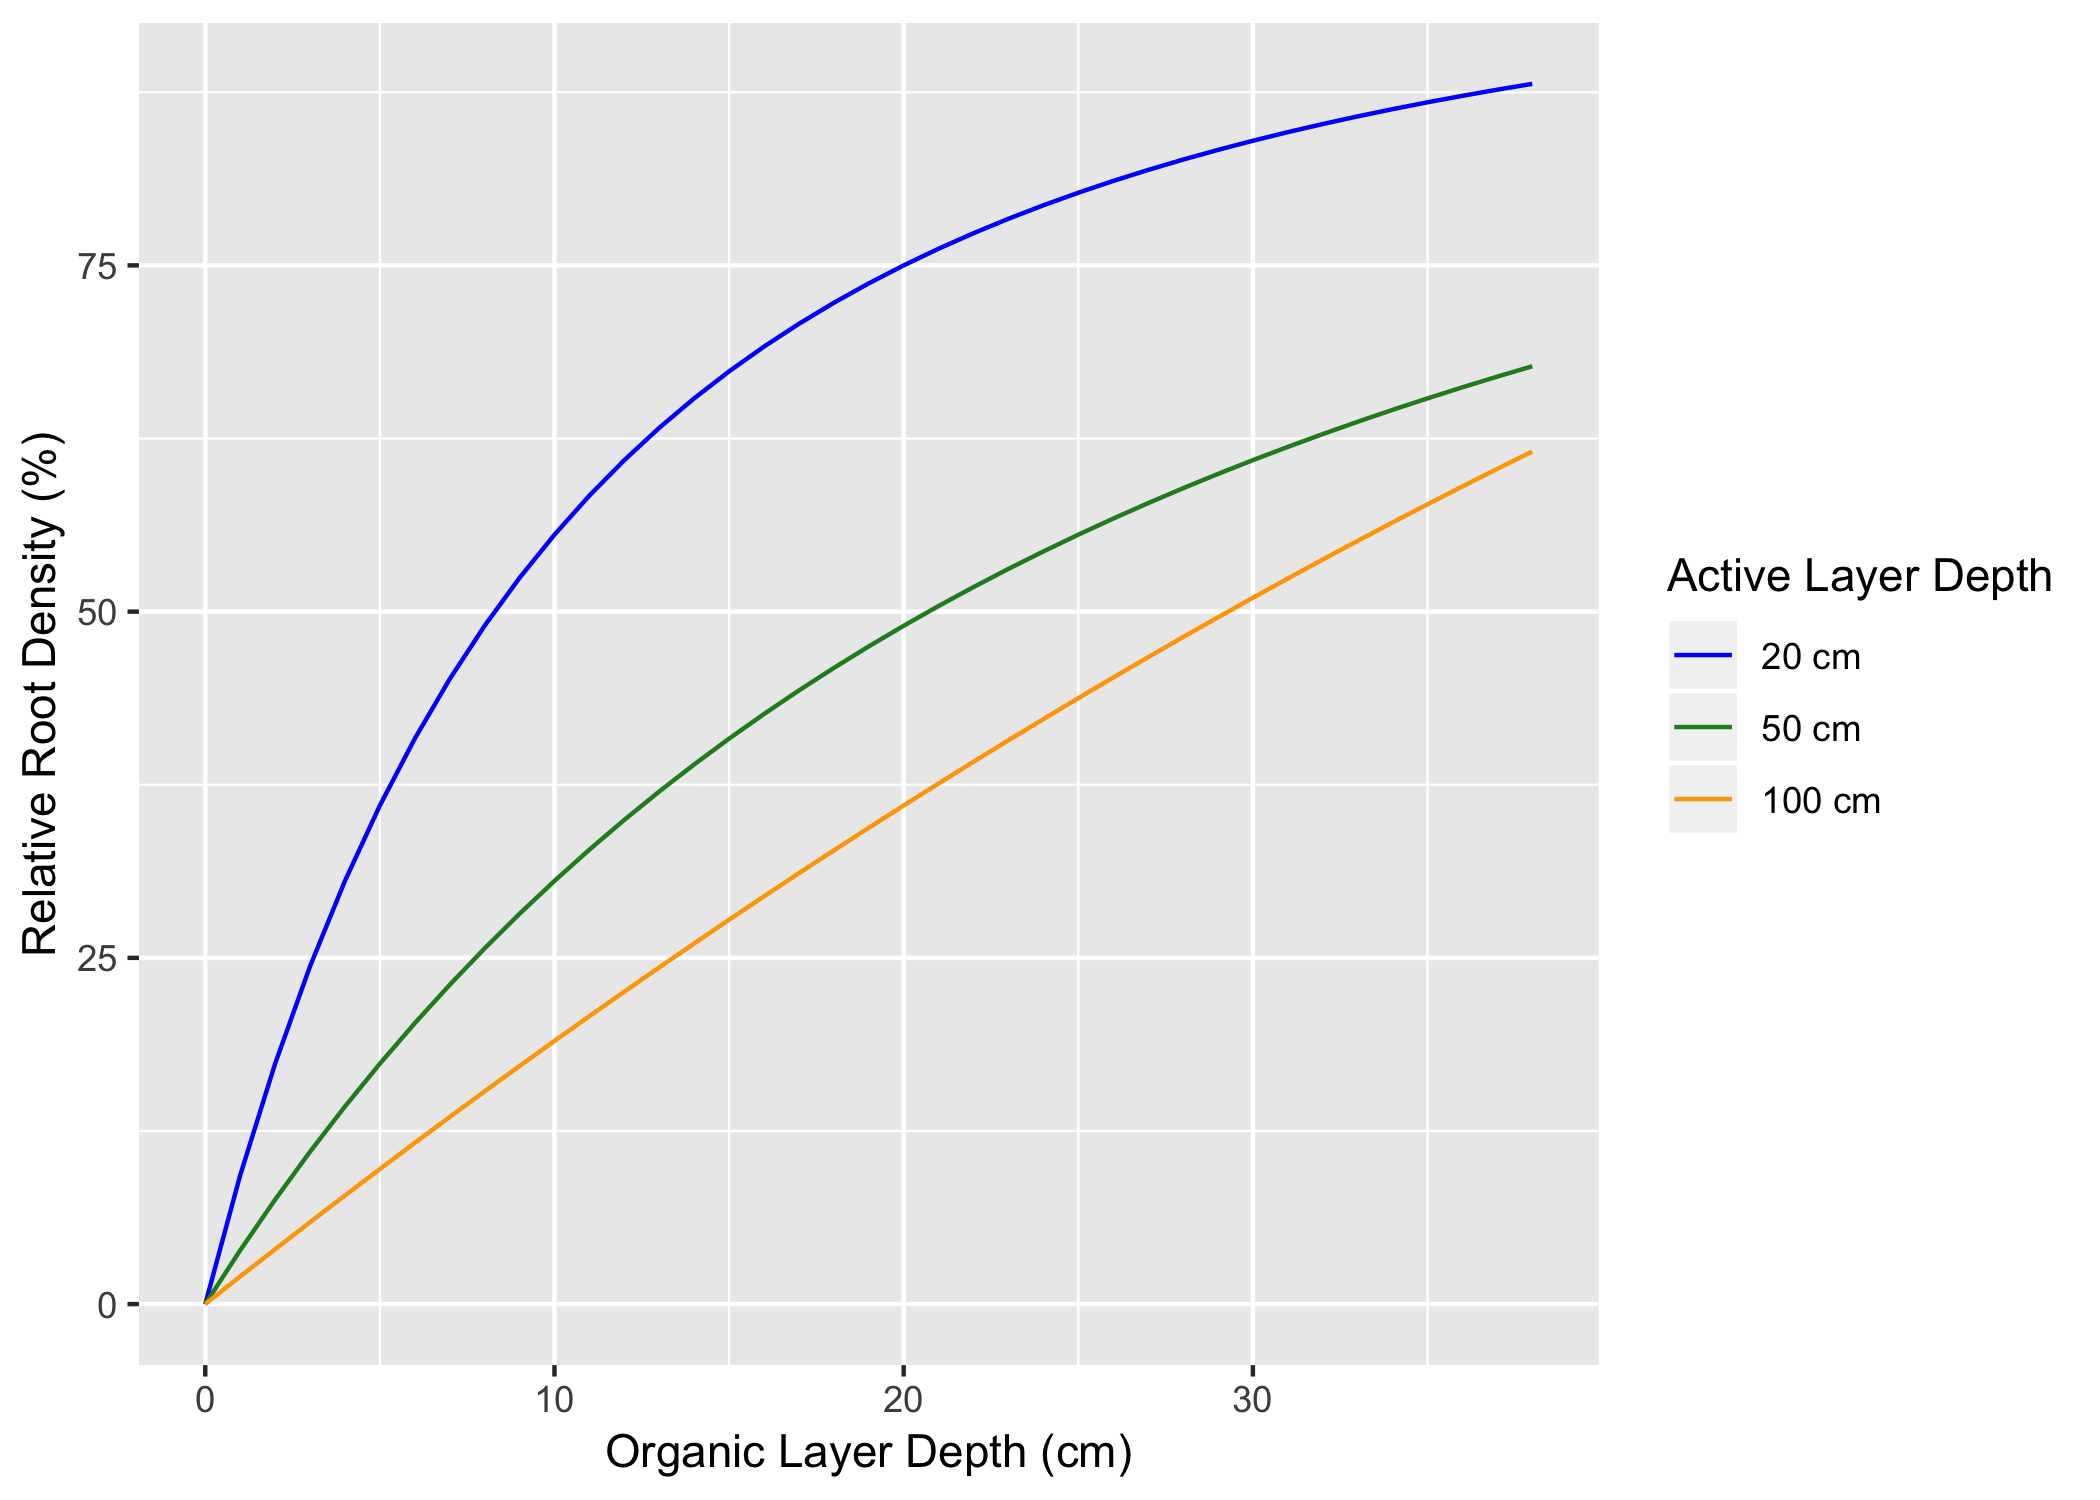
\includegraphics[width=0.8\linewidth]{Figures/RootDens.png}
  \caption{Relative root density in the organic layer with changing organic layer and active layer depths (Eq. \ref{rooteq}).}
  \label{fig:roots}
\end{figure}

The potential water loss from each soil layer is then calculated as:

\begin{equation} \label{pwl1}
pwl_{org} = \min(pw \times r_z, 0.0)
\end{equation}

\begin{equation} \label{pwl2}
pwl_{min} = \min\Big(pw(1.0 - r_z), 0.0\Big)
\end{equation}

Actual water loss from each layer ($E_s$, m) is calculated using an exponential equation for water retained for a given evaporative demand from \citeA{pastorDevelopmentLinkedForest1985, pastorCalculatingThornthwaiteMather1984} and \citeA{bonanComputerModelSolar1989}:

\begin{equation}
E_s= w_l - w_l{\rm e}^{B|pwl_s|}
\end{equation}

where $pwl_s$ is the potential water loss from the layer (Eq. \ref{pwl1}-\ref{pwl2}), and $B = 0.461 - 1.10559/(z_{drain}d_s)$. Finally, the amount of liquid water that freezes in each later ($w_f$, m) is calculated. As in \citeA{bonanComputerModelSolar1989}, water freezes in proportion to the change depth of freezing (Section \ref{perm}):

\begin{equation}
w_f= \Big(\frac{w_l}{d_{thaw}}\Big)(d_{freeze} - d'_{freeze})
\end{equation}

where $d_{freeze}$ is the current day's depth of freezing (m) and $d'_{freeze}$ is the previous day's depth of freezing (m). This amount is subtracted from the liquid water pool and added to the frozen water pool (Fig. \ref{fig:icewater}).

\begin{figure}
  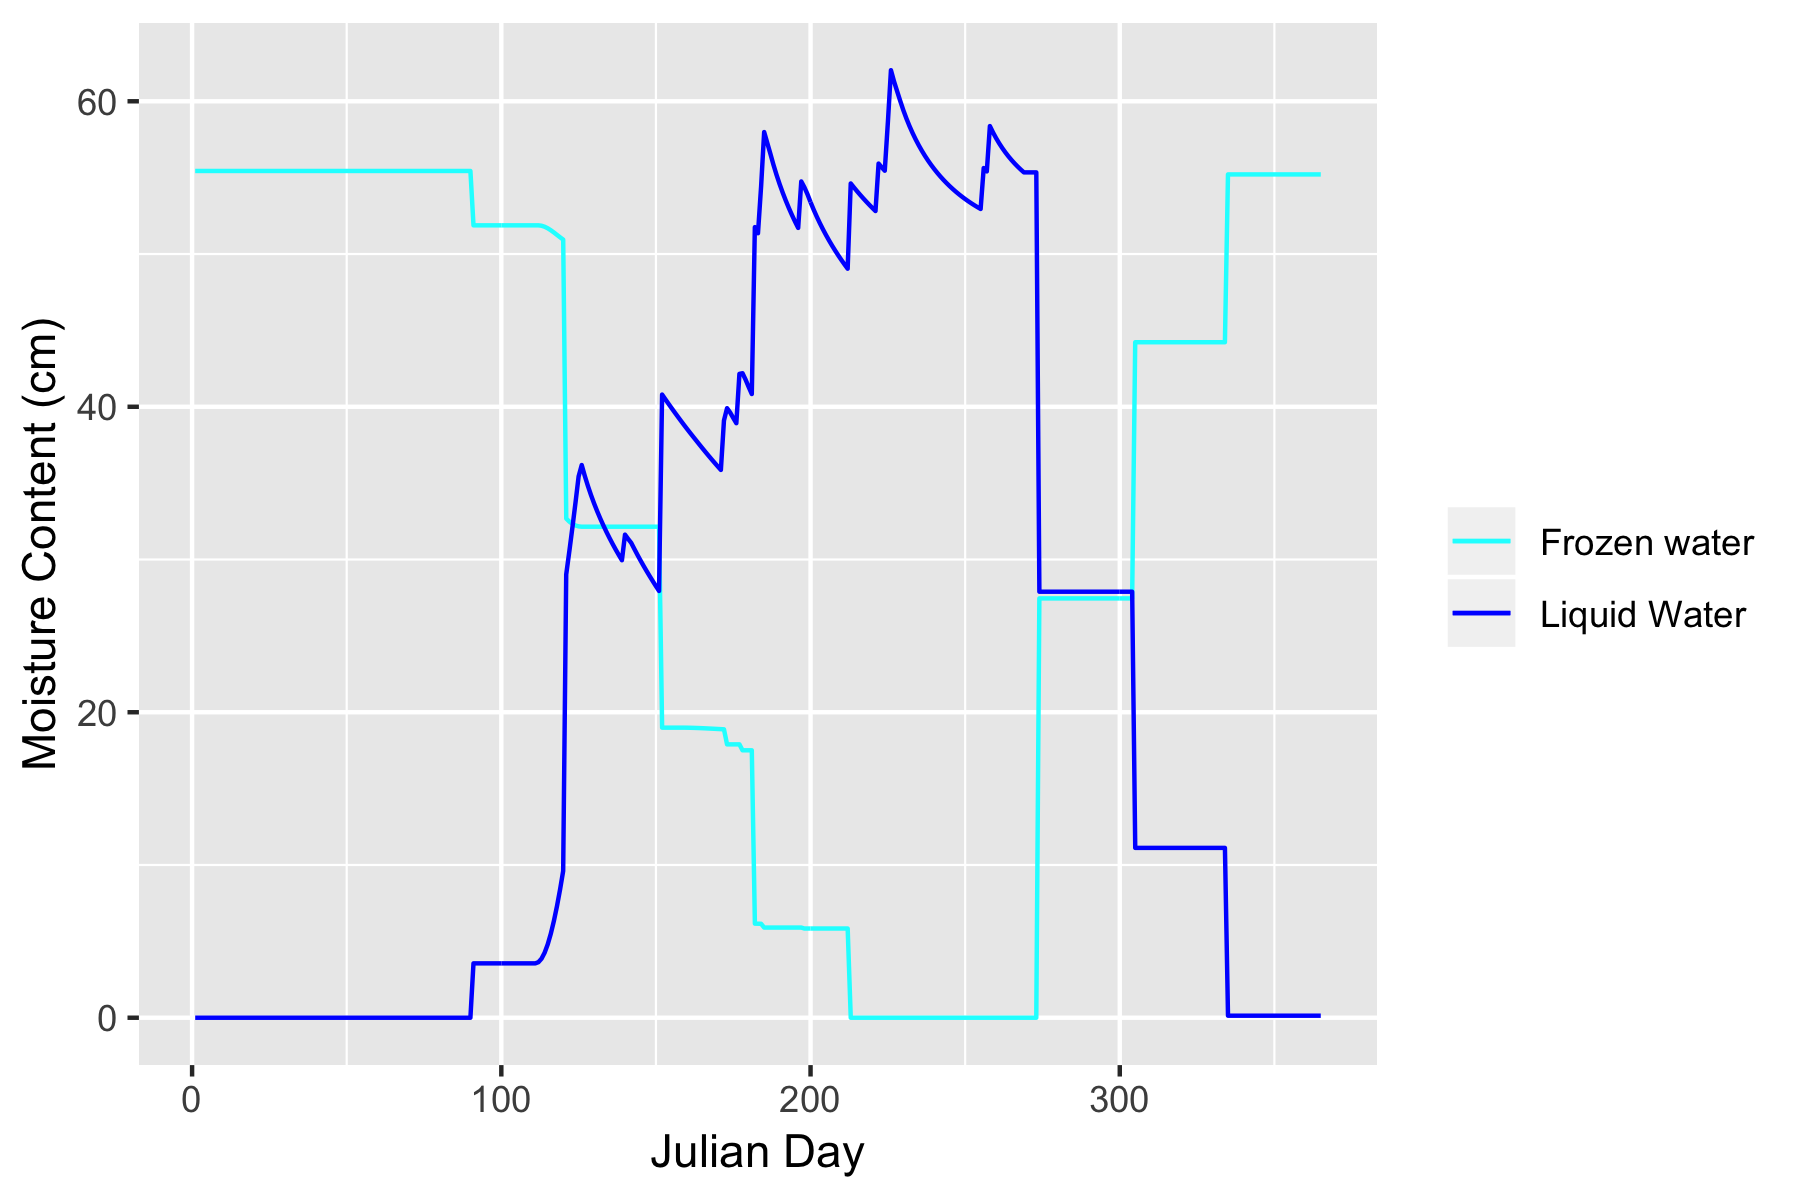
\includegraphics[width=0.8\linewidth]{Figures/Ice.png}
  \caption{Example simulation of frozen and liquid water amounts in the soil (cm) throughout a simulation year for a site in interior Alaska.}
  \label{fig:icewater}
\end{figure}

Total runoff for that day ($R_{tot}$, m) is calculated as the sum of excess water from the soil and that due to slope runoff (Eq. \ref{slr}):

\begin{equation}
R_{tot} = w_{exs_{min}} + R_s
\end{equation}

Total AET (m) is calculated as evaporation from the canopy and soil layers (Fig. \ref{fig:aet}):

\begin{equation}
AET = E_{can} + E_{org} + E_{min}
\end{equation}

The daily soil water contents are used to calculate daily indices of soil dryness and saturation which are aggregated to create annual drought and saturation indices, used throughout the rest of the simulation. In this updated version, organic and mineral layer water contents are scaled by the updated wilting point and field capacity (i.e. $m'_{pwp}$ and $m'_{fc}$, Eqs. \ref{ms} - \ref{mpw}), rather than by the static input values (see Section \ref{growth}). Note: when the thaw depth is greater than the soil layer depth, this scaling would not impact the input wilting point and field capacity values.

\begin{figure}
  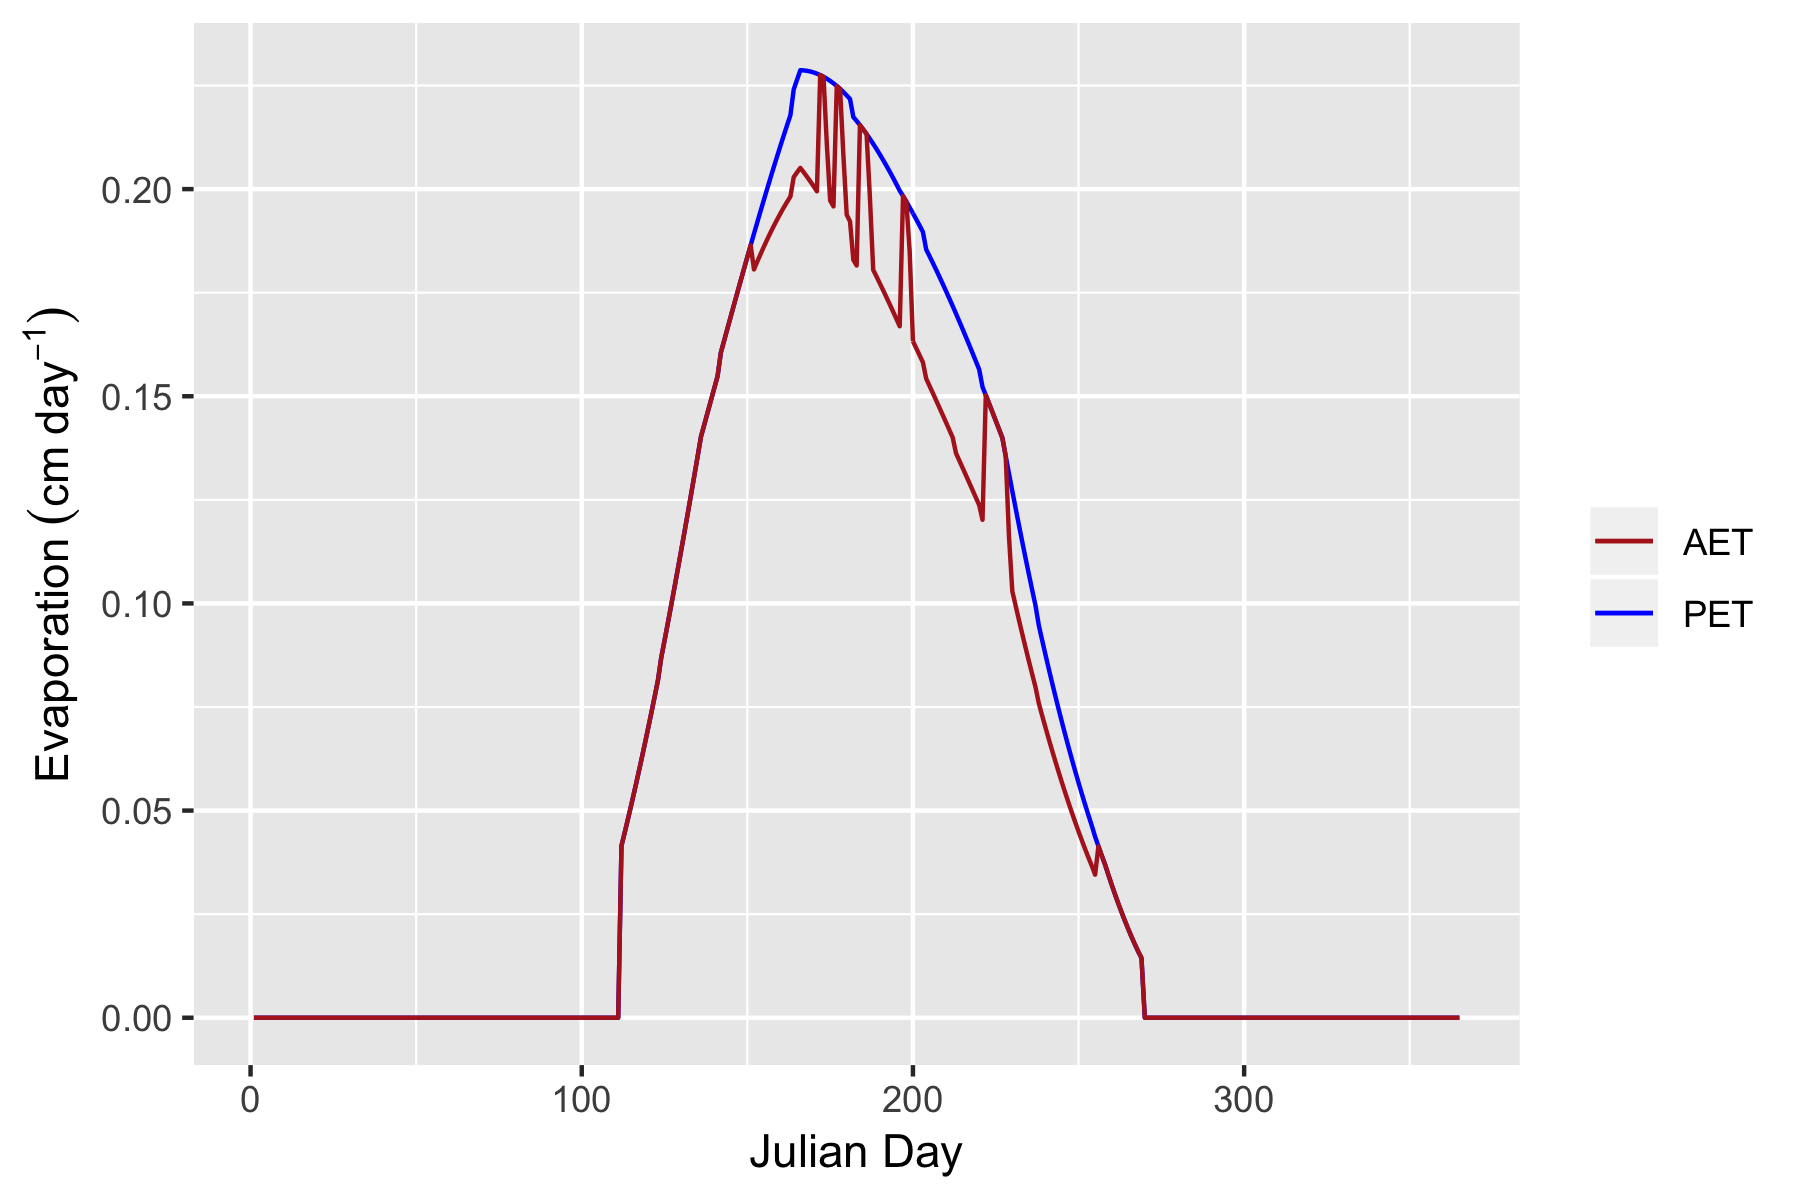
\includegraphics[width=0.8\linewidth]{Figures/AET.png}
  \caption{Example simulation of AET and PET for a site in interior Alaska.}
  \label{fig:aet}
\end{figure}

\subsection{Soil Decomposition and Soil Nutrients} \label{nutrients}
In previous versions of UVAFME, any plants that died and all annual litterfall were added to site-wide pools of C and N, regardless of litter type (i.e. boles, leaves, etc.) or species \cite{fosterValidationApplicationForest2017, yanFAREASTForestGap2005}. These C and N amounts along with temperature and soil moisture were used to calculate soil respiration and plant-available nitrogen. This previous submodel was based on the CENTURY model's soil nutrient cycling \shortcite{partonGeneralModelSoil1994} and performed well in simulating vegetation-soil interactions in previous applications of UVAFME \cite{yanFAREASTForestGap2005, shumanFireDisturbanceClimate2017, fosterValidationApplicationForest2017}. The updated version described below allows for finer-scale interactions between climate, soils, vegetation, and disturbances through explicit tracking and decomposition of individual forest litter ``cohorts". Within the simulation, any litter from branch thinning, annual leaf-off, or plant mortality is added to a litter array along with moss litter (see Section \ref{moss}), depending on its type and genus (for leaf litter). Litter is accumulated within the array throughout each simulation year and decomposed the following year in the updated soil decomposition subroutine (Fig. \ref{fig:nutrientdiagram}).

For bare-ground initiation runs, it is assumed that a severe fire has initiated secondary succession and thus some amount of litter and humus remain at the site. For each plot to be simulated, woody litter is initialized to a default amount of 53.5 t ha$^{-1}$, whereas all other litter types (i.e. leaves, twigs, roots, well-decayed wood, and moss) remain at 0.0 t ha$^{-1}$. Organic matter (humus) is initialized to 75 t ha$^{-1}$, and humus N content is initialized to 0.6 t ha$^{-1}$, as in Bonan (1990). Initial organic layer depth ($d_{org}$, m) is then calculated as \shortcite{keaneFireBGCv2LandscapeFire2011}:

\begin{equation}
d_{org} = (1/plotsize)(\frac{M_{hum}}{bd_{hum}})
\end{equation}

where $plotsize$ is the plot area (default to 500 m$^2$), $M_{hum}$ is the amount of humus (kg plot$^{-1}$), and $bd_{hum}$ is the bulk density for humus, set to a default value of 76.94 kg m$^{-3}$ as in \citeA{bonanCarbonNitrogenCycling1990}.

\subsubsection{Litter Cohorts and Characteristics}
In this updated nutrient submodel, different types of litter decay at different rates according to input litter characteristics. Each year, litter from each of these different types is placed into separate cohorts which decay until they reach a critical weight at which they are transferred to either humus or well-decayed wood (Fig. \ref{fig:nutrientdiagram}). Input litter parameters (Table \ref{tab:litterparms}) are taken from \citeA{pastorDevelopmentLinkedForest1985} and \citeA{bonanCarbonNitrogenCycling1990}.

\begin{figure}
  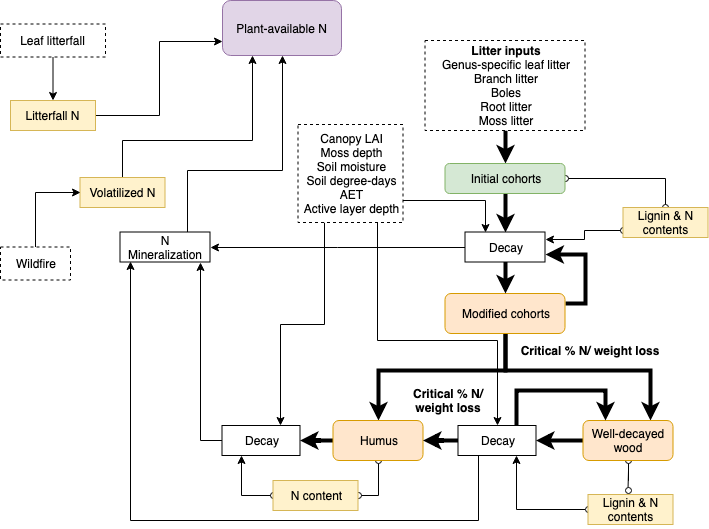
\includegraphics[width=\linewidth]{Figures/SoilNutrients.png}
  \caption{Flow diagram showing litter and decomposition dynamics simulated in UVAFME.}
  \label{fig:nutrientdiagram}
\end{figure}

\begin{table}
 \begin{center}
    \caption{Input litter parameters. Values taken from \protect\citeA{pastorDevelopmentLinkedForest1985} and \protect\citeA{bonanCarbonNitrogenCycling1990}.}
    \label{tab:litterparms}
 \resizebox{\textwidth}{!}{\csvautotabular{UVAFME2018_litterpars.csv}}
\end{center}
\end{table}

The ash parameter ($\alpha$) is a correction factor to calculate ash-free weight of litter from the initial input weight. This value is multiplied by the initial cohort's weight at the beginning of decomposition. The initial N parameter, $pN_{init}$ is the proportion of the litter cohort's weight that is nitrogen. This value is multiplied the the cohort's initial ash-free weight to derive initial N weight ($N_{init}$, tN ha$^{-1}$). The immobilization parameter determines how much N (g) is immobilized per gram weight loss of the litter type, and is used to decrease the N content of decaying litter and to calculate total N immobilized during decomposition. The critical N parameter ($pN_{crit}$) is the critical proportion of N at which a decaying litter cohort is transferred to either well-decayed wood (for boles) or humus (all other litter types). The initial lignin parameter ($pL_{init}$) is the litter cohort's initial lignin percent. The initial lignin percent is also used to calculate the critical fraction remaining ($pM_{crit}$) at which a decaying litter cohort is transferred to humus or well-decayed wood:

\begin{equation}
pM_{crit} = 1.7039pL_{init} + 0.0955
\end{equation}

Finally, the parameters $A$ and $B$ are used to update litter lignin percent as the litter cohort decays.

\subsubsection{Litter Decay}

Cohort decay is dependent on different site conditions such as litterfall rate, light level, moisture, permafrost depth, moss cover, as well as litter characteristics.  A factor to incorporate the effects of canopy gaps on litter decay ($f_g$) is calculated as in \citeA{pastorDevelopmentLinkedForest1985} that depends on actual litterfall relative to a closed canopy litterfall variable. Closed canopy litterfall is calculated as:

\begin{equation}
P_{can} = 1.54 + 0.0457(w_{fc} - w_{pwp})
\end{equation}

where $w_{fc}$ and $w_{pwp}$ are the combined field capacities and wilting points of the organic and mineral layers (cm). The total leaf litter that year ($l_{leaves}$, t ha$^{-1}$) along with $P_{can}$ is used to calculate the canopy gap factor (Fig. \ref{fig:flit}):

\begin{equation} \label{fliteq}
f_{g} = \begin{cases}
1.0 + \Big(-0.5 + 0.075(w_{fc} - w_{pwp})\Big)\Big(1.0 - \frac{l_{leaves}}{P_{can}}\Big), & \text{$l_{leaves} \leq P_{can}$}. \\
1.0, & \text{$l_{leaves} > P_{can}$}.
\end{cases}
\end{equation}

As the actual litterfall decreases relative to the calculated closed canopy litterfall amount, $f_g$ increases and thus acts to increase litter decay rate (Eq. \ref{ppeq}).

\begin{figure}
  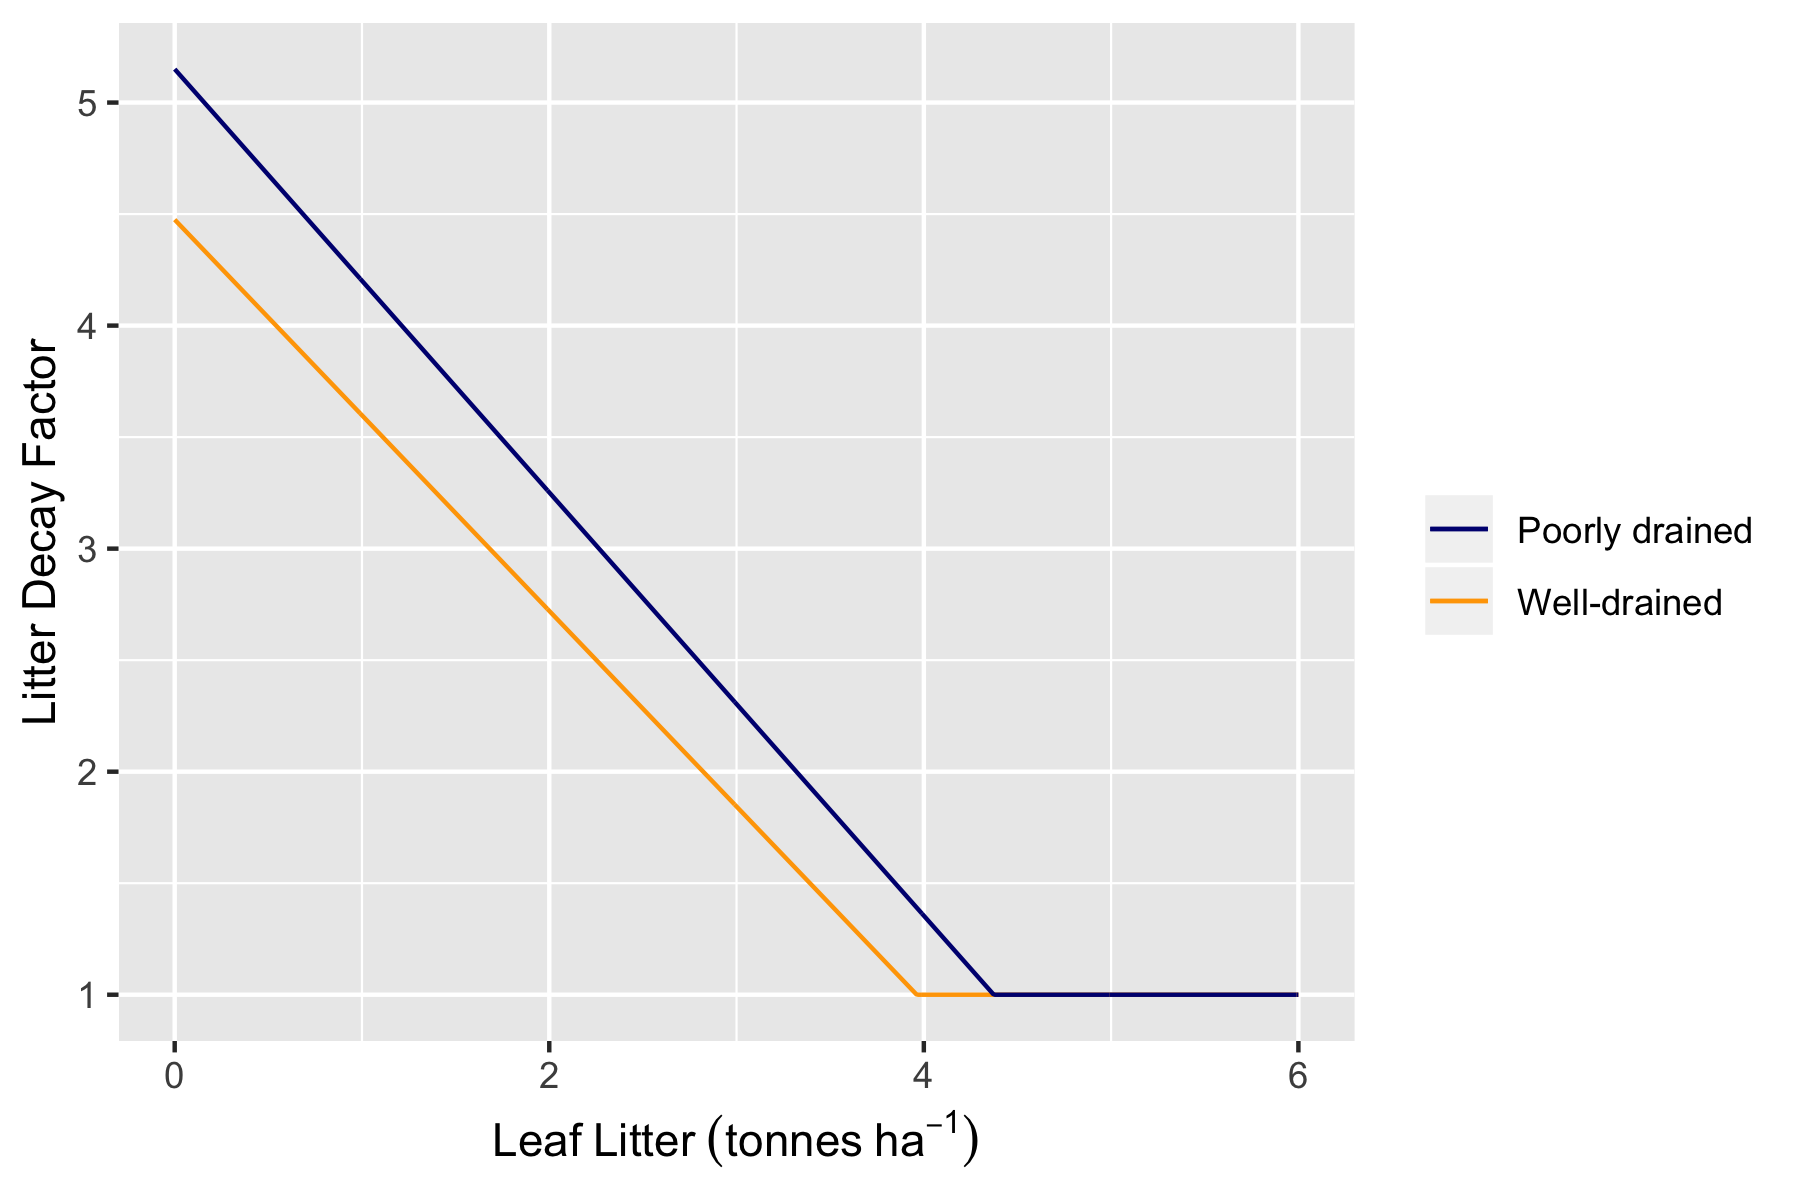
\includegraphics[width=0.9\linewidth]{Figures/Flit.png}
  \caption{Example calculation for the litter decay factor ($f_g$) for a poorly drained ($w_{fc} =$ 68 cm) and well-drained ($w_{fc} =$ 59 cm) site (Eq. \ref{fliteq}).}
  \label{fig:flit}
\end{figure}

An additional light level decay multiplier from \citeA{bonanCarbonNitrogenCycling1990} is used that incorporates LAI:

\begin{equation} \label{flai}
f_{LAI} = \begin{cases}
1.0, & \text{$LAI \ge 2.5$}. \\
1.0 + 1.5\sqrt{1.0 - LAI/2.5}, & \text{$LAI < 2.5$}
\end{cases}
\end{equation}

As in the previous equation, as LAI decreases, the LAI factor increases above 1.0 (Fig. \ref{fig:fLAI}), thus increasing the decay rate (Eq. \ref{bbeq}).

\begin{figure}
  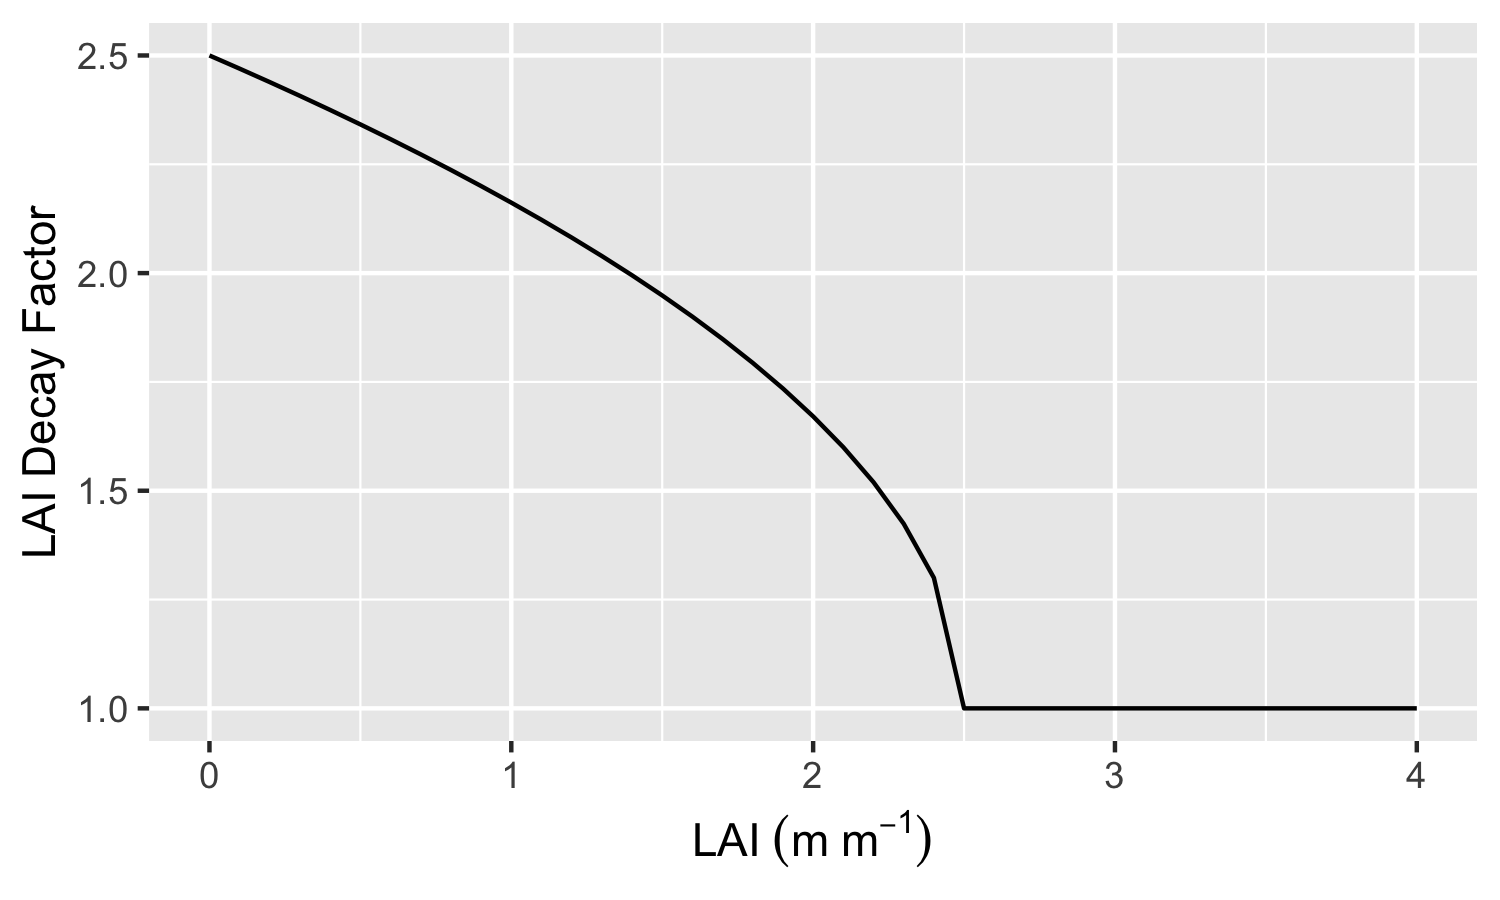
\includegraphics[width=0.9\linewidth]{Figures/fLAI.png}
  \caption{The LAI decay factor ($f_{LAI}$) increases with decreasing LAI; Eq. \ref{flai} \protect\cite{bonanCarbonNitrogenCycling1990}.}
  \label{fig:fLAI}
\end{figure}

As in previous versions of UVAFME, a soil moisture factor ($f_{moist}$) is used to simulate the effects of soil moisture on decomposition \cite{fosterValidationApplicationForest2017}. In this updated version moss depth is also incorporated into this factor. 

\begin{equation} \label{mossmoist}
  \begin{aligned}
f_{moist} = 0.5\Bigg[ & \max\Big(1.6 - \sqrt{4(d_{moss} + d_{mlitter})}, 0.0\Big) + \\
  & \max\Big(3(1 - 1.25SI)^2, 0.2\Big)\Bigg]
 \end{aligned}
\end{equation}

where $d_{moss}$ and $d_{mlitter}$ are the depths of live moss and moss litter (cm), and $SI$ is a saturation index, based on the percent of the growing season with mineral soil moisture above field capacity. As the saturation index increases and moss depth increases, $f_{moist}$ decreases (Fig. \ref{fig:moistfig}), thus impacting litter decay.

\begin{figure}
  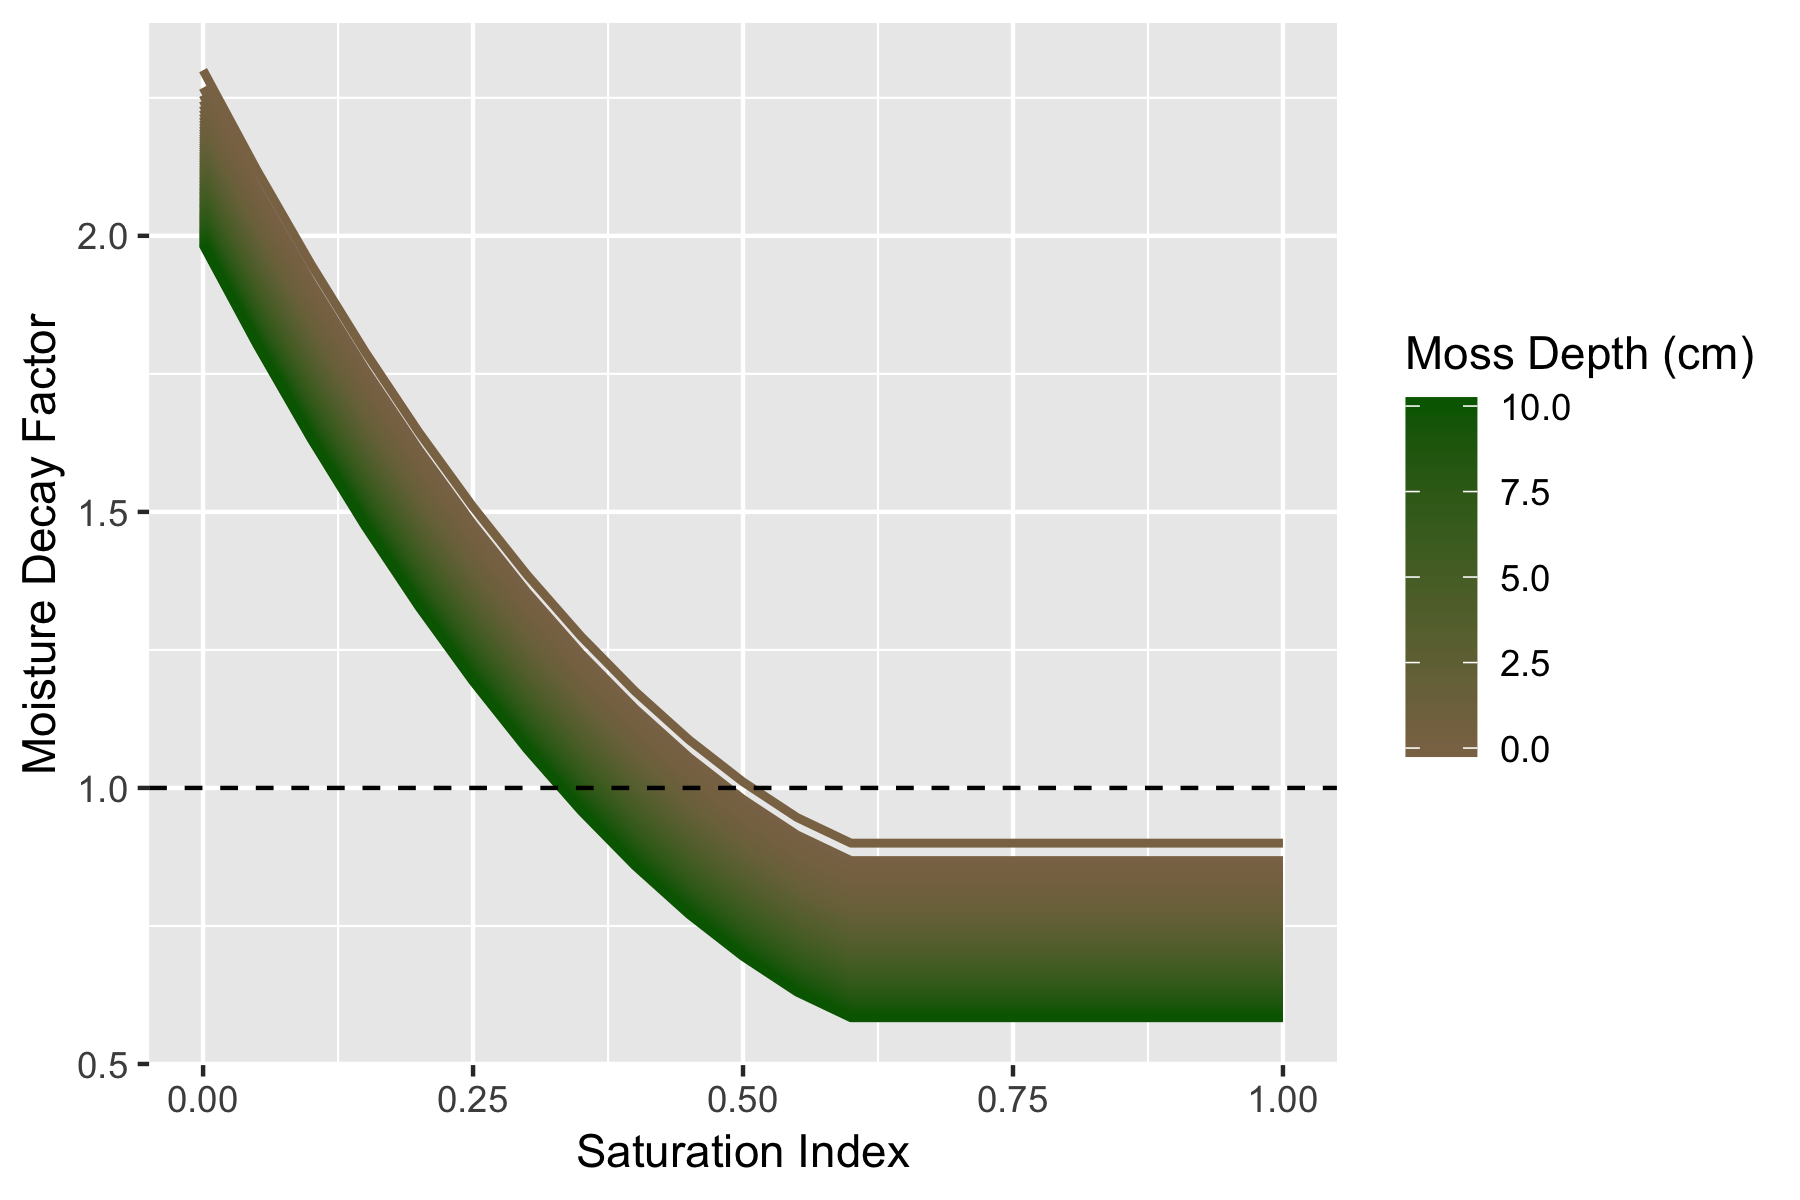
\includegraphics[width=0.9\linewidth]{Figures/MossMoistFact.png}
  \caption{The moisture decay factor ($f_{moist}$) decreases with increasing saturation and increasing moss depth (Eq. \ref{mossmoist}).}
  \label{fig:moistfig}
\end{figure}

The temperature decay factor ($f_{temp}$) from the previous version of UVAFME is modified for this updated version as:

\begin{equation} \label{tempdecay}
f_{temp} = 2^{0.005(SD - 1950)}
\end{equation}

where $SD$ is soil degree-days (cumulative sum of temperatures above 0ºC). This equation is based on a temperature coefficient Q$_{10}$ relationship, with parameters estimated using decay rates from a litterbag study by \citeA{yarieLitterbagDecompositionStudy1997} (Fig. \ref{fig:tempfact}).

\begin{figure}
  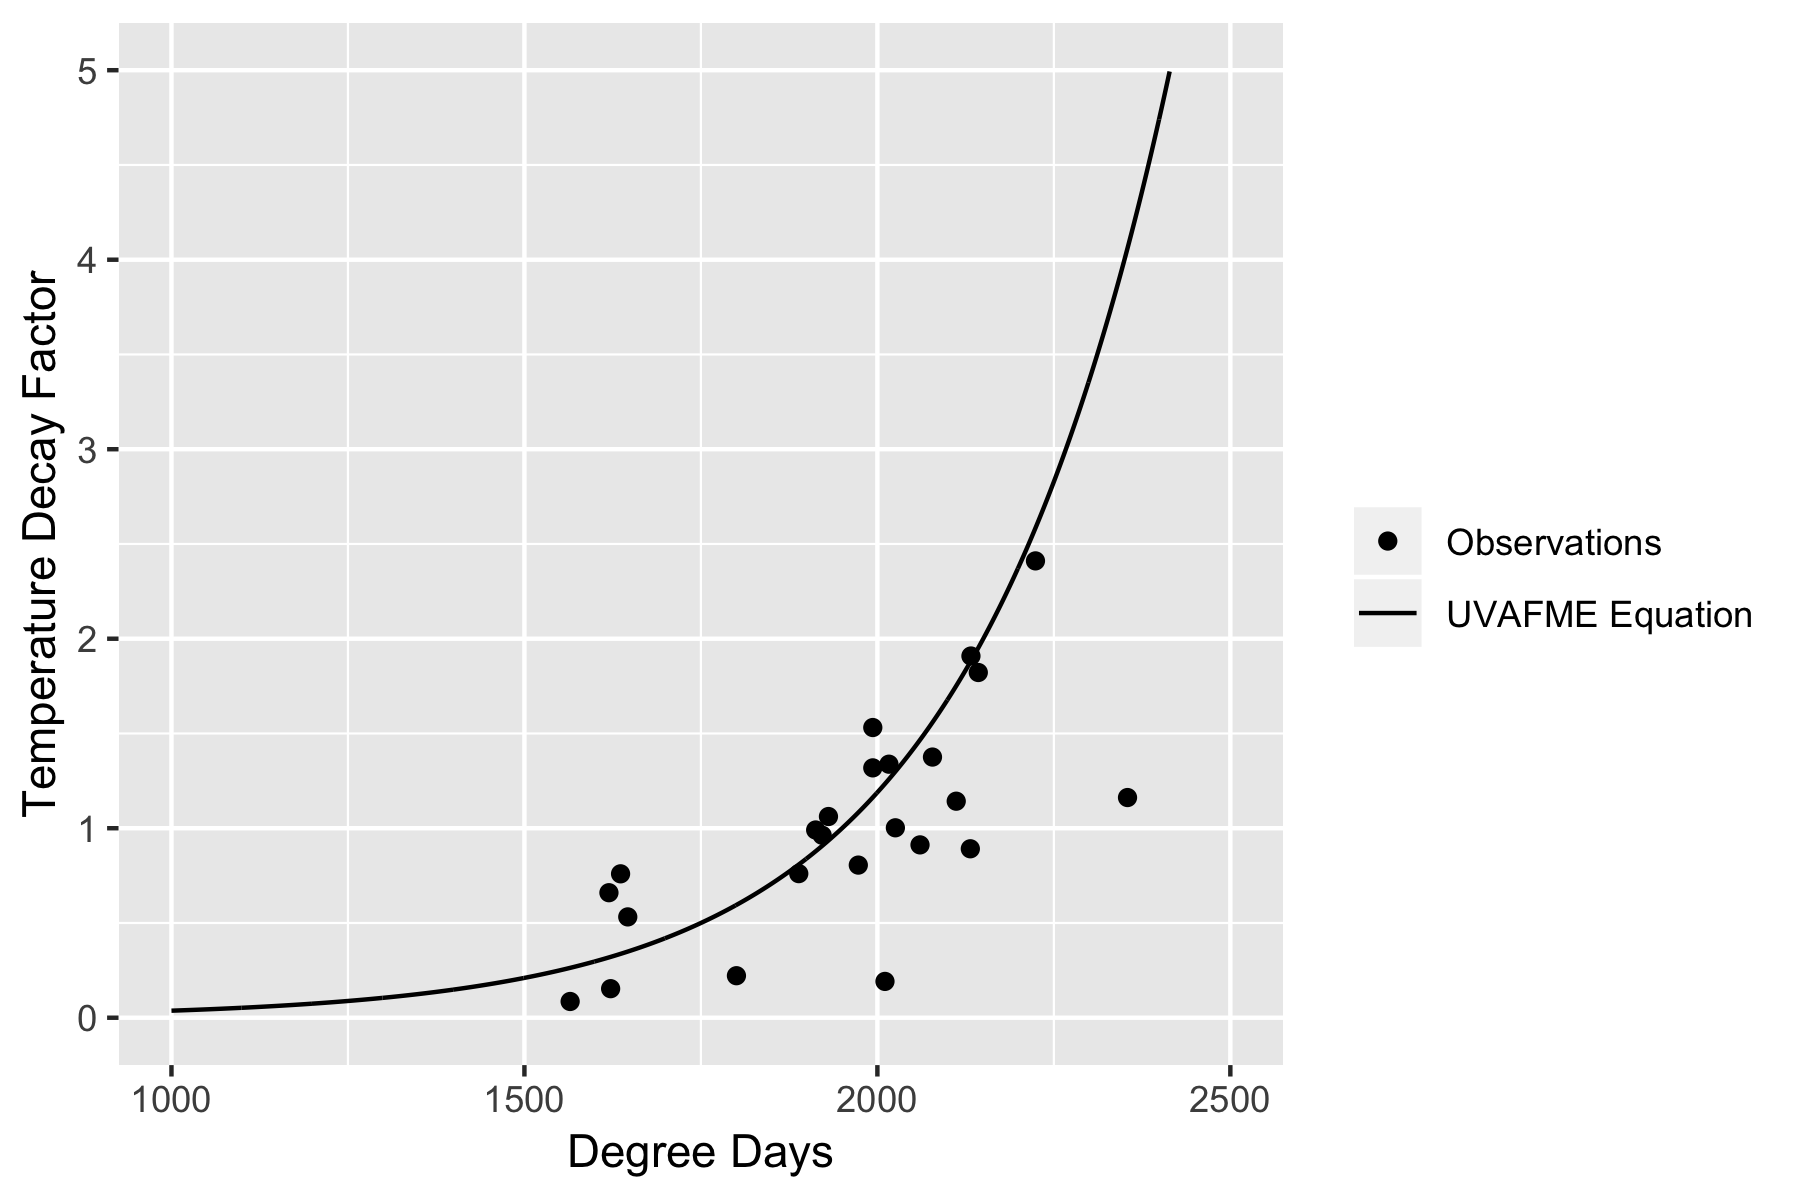
\includegraphics[width=0.8\linewidth]{Figures/TempFact.png}
  \caption{Annual decay rates normalized by average decay rate versus degree-days above 0ºC along with the UVAFME temperature decay factor (Eq. \ref{tempdecay}). Observation data are from a litterbag study from 1989 to 1997 at several Bonanza Creek LTER sites \protect\cite{yarieLitterbagDecompositionStudy1997} and from temperature data from the same sites and years \protect\cite{vancleveBonanzaCreekLTER2017}.}
  \label{fig:tempfact}
\end{figure}

Percent weight loss ($pM_{loss}$) is then calculated as a function of these multipliers in addition to other site-level metrics. For this updated version a combination of two different equations for percent weight loss is used from \citeA{pastorDevelopmentLinkedForest1985} and \citeA{bonanCarbonNitrogenCycling1990}. Pastor and Post's equation uses $f_g$ as well as site-level evapotranspiration ($AET$, mm), and the lignin:N ratio of the litter to calculate annual percent weight loss:

\begin{equation} \label{ppeq}
  \begin{aligned}
pM_{lossPP} = 0.01f_g\Bigg(\Big(0.9804 + 0.09352AET\Big) - \\
		\Big(pL:pN(-0.4956 + 0.00193AET)\Big)\Bigg)
\end{aligned}
\end{equation}

where $pL$ and $pN$ are the cohort's current percent lignin and percent N. Bonan's equation uses the percent N of the litter as well as $f_{LAI}$ and active layer depth ($alt$, m):

\begin{equation} \label{bbeq}
pM_{lossB} = f_{LAI}\Big((-0.0052 + 2.08pN)\text{e}^{0.898alt}\Big)
\end{equation}

In this updated version, if the active layer depth is less than 1.5 m, the percent weight loss ($pM_{loss}$) is calculated as an average of Bonan's (Fig. \ref{fig:bon}) and Pastor and Post's equation (Fig. \ref{fig:pp}), otherwise only Pastor and Post's equation is used (note: for decay of moss litter, only Bonan's equation is used, regardless of active layer depth).

\begin{figure}
  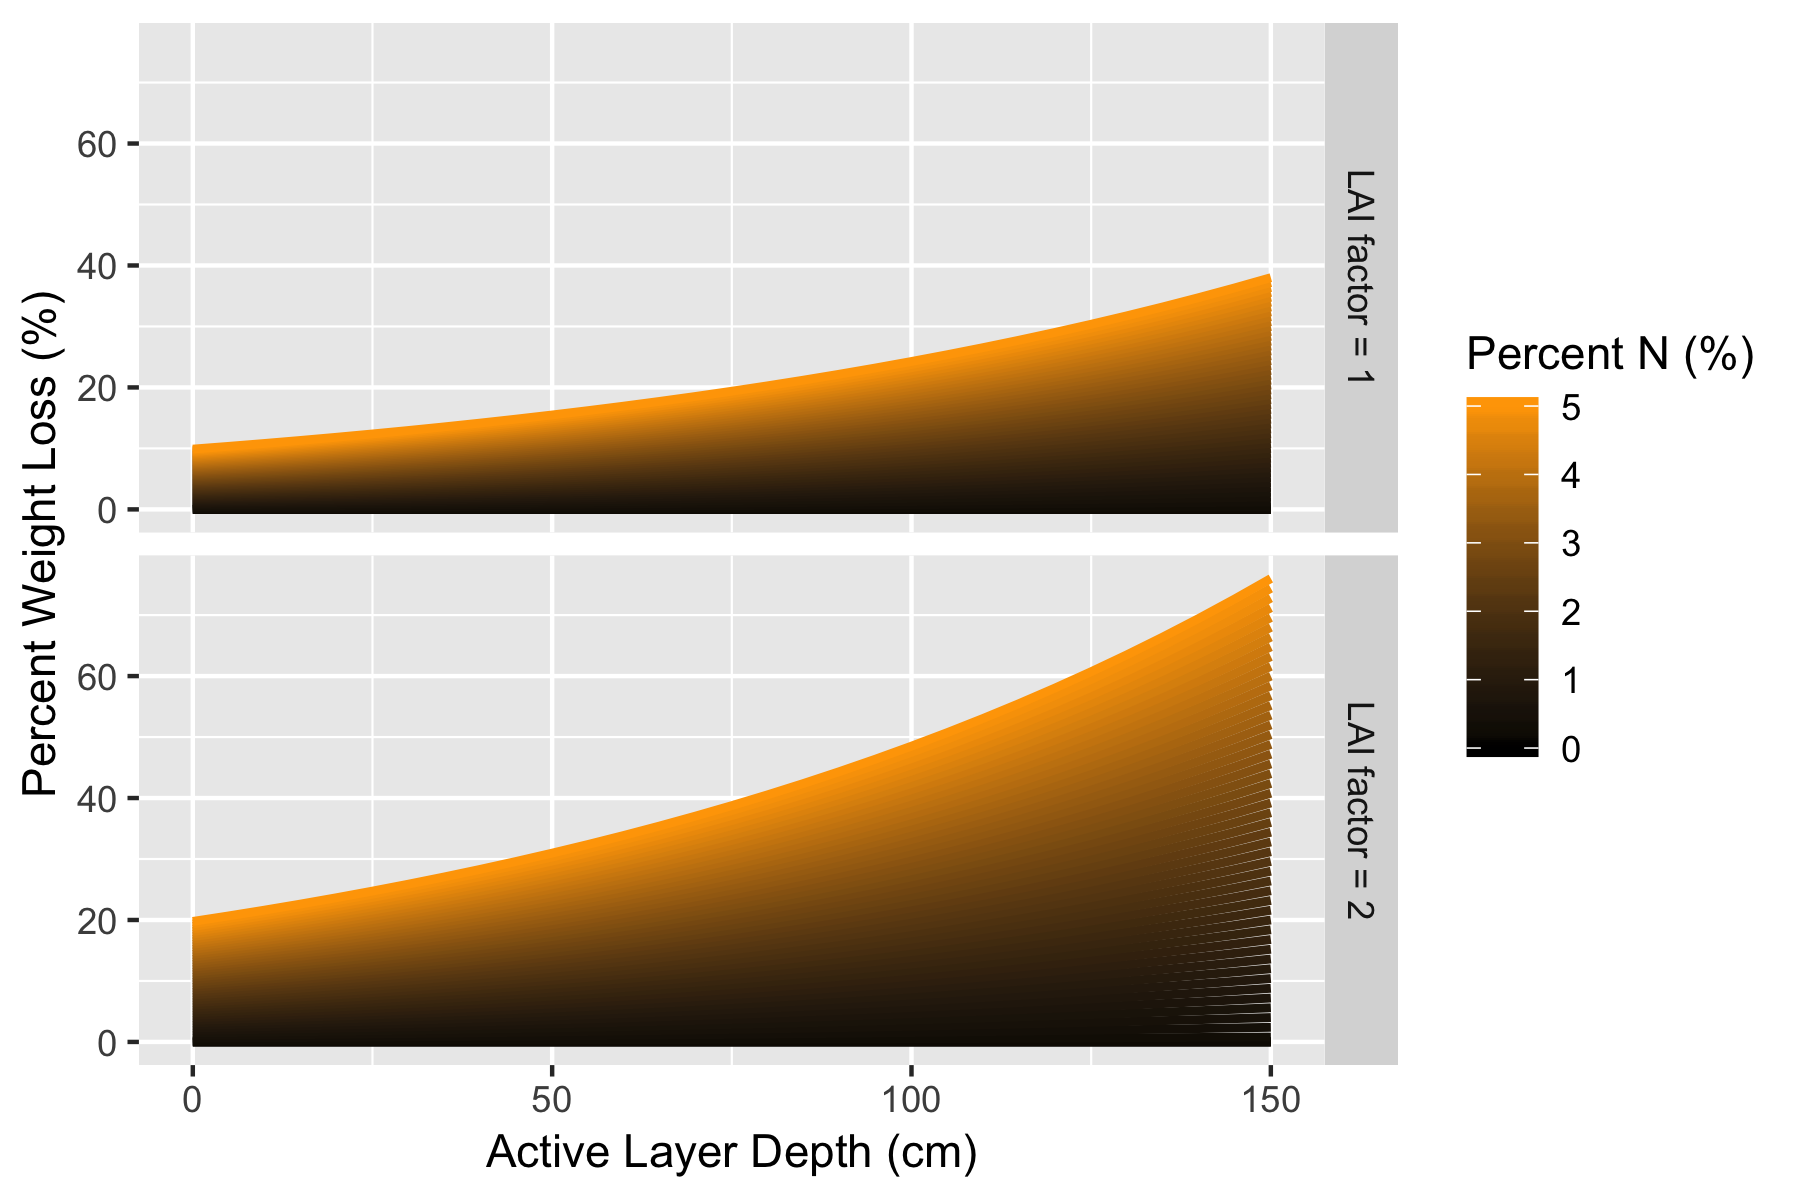
\includegraphics[width=0.8\linewidth]{Figures/Bonan.png}
  \caption{Example calculation of percent weight loss from \protect\citeA{bonanCarbonNitrogenCycling1990} (Eq. \ref{bbeq}).}
  \label{fig:bon}
\end{figure}

\begin{figure}
  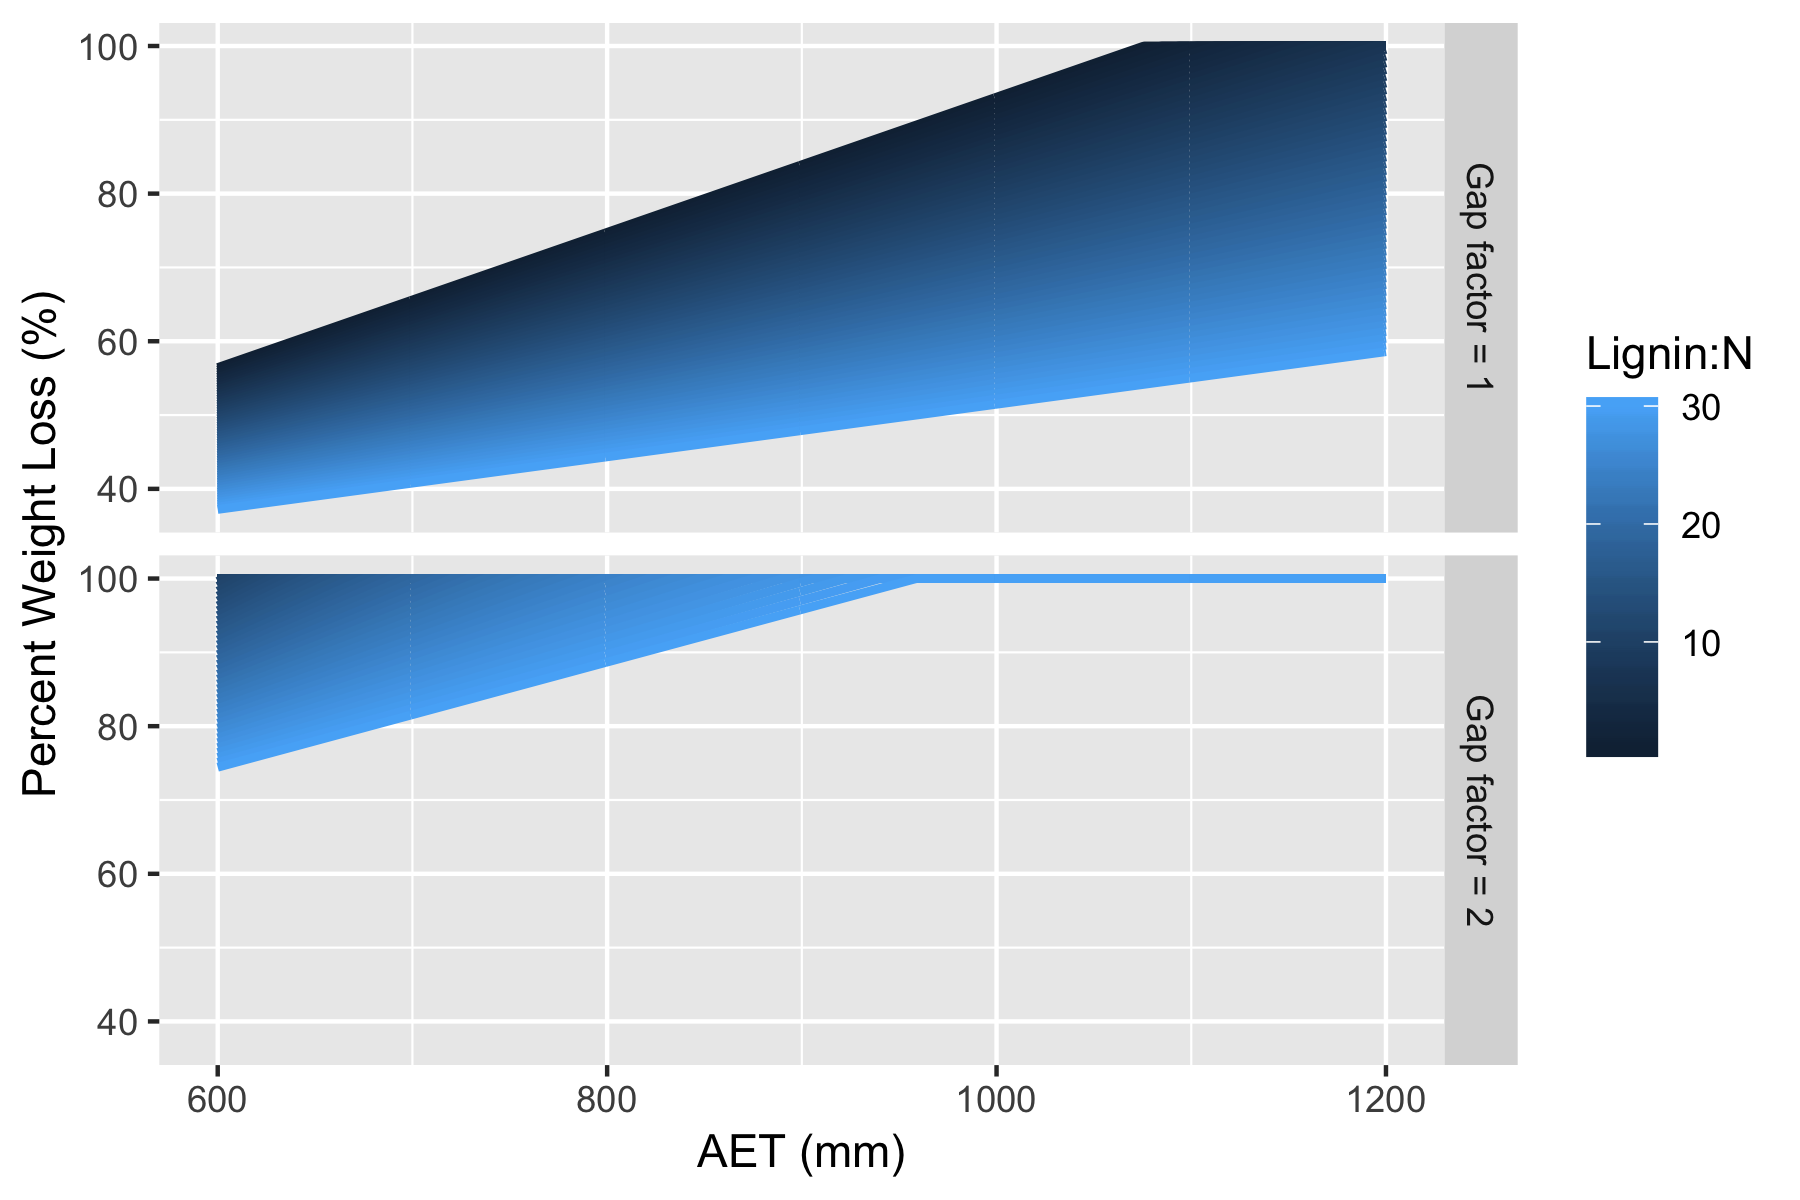
\includegraphics[width=0.8\linewidth]{Figures/PP.png}
  \caption{Example calculation of percent weight loss from \protect\citeA{pastorDevelopmentLinkedForest1985} (Eq. \ref{ppeq}).}
  \label{fig:pp}
\end{figure}

These percent weight loss calculations are then modified as: $pM_{loss} = \min\Big(\max(pM_{loss}f_{temp}f_{moist}, 0.0), 1.0\Big)$, and further modified as in \citeA{pastorDevelopmentLinkedForest1985}  such that the weight loss of large boles is 3\%, weight loss of small boles is 10\%, weight loss of well-decayed wood is 5\%, and weight loss of twigs is a maximum of 20\%.

The actual weight loss is calculated as the percent weight loss times the current weight of the litter cohort ($M_{loss} = pM_{loss}M$), and the fraction of the original input organic matter remaining is then calculated as:

\begin{equation} 
pM_{rem} = (M - M_{loss})/M_{init}
\end{equation}

The new N concentration after weight loss is calculated as:

\begin{equation} 
pN = gN - pN_{crit}pM_{rem}
\end{equation}

where $gN$ is an input litter parameter (Table \ref{tab:litterparms}) representing the grams of N immobilized per gram weight loss. These values are used to determine if each cohort will remain to decay further the following year or if the remaining organic matter will be transferred to humus or well-decayed wood. If the percent remaining is less than the critical fraction remaining ($pM_{crit}$), then the cohort is transferred. When this occurs, the actual weight loss and N concentration are recalculated as:

\begin{equation} 
M_{loss} = M - pM_{crit}M_{init}
\end{equation}

and

\begin{equation} 
pN = gN - pN_{crit}pM_{crit}
\end{equation}

The absolute change in N content as a result of decay is calculated as the difference between the N content before this year's decay and the N content of the litter cohort as a result of this year's decay: $\delta N = M_N - pN(M - M_{loss})$. If this value is negative, then the total year's N immobilization is increased by $|\delta N|$, otherwise the total year's N mineralization is increased by $\delta N$. The final weight and N content of these cohorts are then transferred to either humus (all litter except boles) or well-decayed wood (boles). For moss litter, transferal to humus is calculated using critical weight loss rather than critical percent remaining, as in \citeA{bonanCarbonNitrogenCycling1990}. Critical weight loss is calculated as the weight loss required for the current N concentration to equal the N concentration at which moss is transferred to humus (Table \ref{tab:litterparms}):

\begin{equation} 
M_{losscrit} = \frac{pN_{crit}M - M_N}{gN + pN_{crit}}
\end{equation}

If the actual weight loss is greater than or equal to the critical weight loss, then the moss cohort is transferred to humus and weight loss is set equal to the critical weight loss amount. The N concentration of the moss cohort is updated to equal the critical N concentration. The N content that is transferred to the humus N pool is then calculated as $M_{loss}gN$ and the remaining moss weight is transferred to the humus pool. The immobilization/mineralization amount is updated as with the other litter cohorts.

If the percent organic matter remaining is greater than the critical percent (for all cohorts but moss), the litter cohort is not transferred and is left to decay further the following year. The current weight and N amount are updated to reflect the weight loss and the lignin concentration is updated as:

\begin{equation} 
pL = A - B\frac{M}{M_{init}}
\end{equation}

where $A$ and $B$ are lignin change parameters (Table \ref{tab:litterparms}). For moss cohorts, if the weight loss is less than the critical weight loss, the cohort is not transferred to humus and the current weight is updated with the weight loss amount. The N content and concentrations are then updated as: $M_N = M_N + M_{loss}gN$ and $pN = M_N/M$.

\subsubsection{Humus Decomposition}

Humus decomposition occurs according to the active layer depth, the N concentration of the humus layer, as well as the previous decay multipliers. When the active layer depth is below 1.5 m, the percent weight loss equation from \citeA{bonanCarbonNitrogenCycling1990} is used, otherwise a separate equation, modified from \citeA{pastorDevelopmentLinkedForest1985} is used:

\begin{equation} 
pM_{loss} = \begin{cases}
f_{moist}f_{temp}f_{LAI}\Big((-0.0052 + 2.08pN)\text{e}^{0.898alt}\Big), & \text{$alt \leq 1.5$} \\
0.035f_gf_{moist}f_{temp}, & \text{$alt > 1.5$}
\end{cases}
\end{equation}

The humus N mineralization is calculated as $N_{hummin} = M_NpM_{loss}$ and the organic and N contents of the humus pools are updated as $M'_{N} = M_N - N_{hummin}$ and $M = M(M'_{N}/M_{N}$). Humus N mineralization and litter cohort mineralization are added together to derive total N mineralization ($N_{min}$) for the year. This value is used to calculate the plant-available N (tN ha$^{-1}$) for the year:

\begin{equation} 
N_{avail} = N_{min} - N_{immob} + N_{fire} + N_{tfall}
\end{equation}

where $N_{fire}$ is volatilized N from fires (see Section \ref{disturbances}), and $N_{tfall}$ is N mineralized from throughfall, set as 16\% of total leaf litter N.

The organic layer depth (m) is then updated as:

\begin{equation}
d_{org} = (1/plotsize)\Bigg(\Big(\frac{M_{con}}{bd_{con}}\Big) + \Big(\frac{M_{dec}}{bd_{dec}}\Big) + \Big(\frac{M_{twigs}}{bd_{twigs}}\Big) + \Big(\frac{M_{moss}}{bd_{moss}}\Big) + \Big(\frac{M_{hum}}{bd_{hum}}\Big)\Bigg)
\end{equation}

where $M_{con}$, $M_{dec}$, $M_{twigs}$, $M_{moss}$ and $M_{hum}$ are the weights of conifer leaf litter, deciduous leaf litter, twig litter, moss litter, and humus (kg plot$^{-1}$), and $bd_{con}$, $bd_{dec}$, $bd_{twigs}$, $bd_{moss}$, and $bd_{hum}$ are their corresponding bulk densities (Table \ref{tab:bulkdens}).

\begin{table}
  \begin{center}
    \caption{Default bulk density values (kg m$^{-3}$) taken from  \protect\citeA{bonanCarbonNitrogenCycling1990}.}
    \label{tab:bulkdens}
\begin{tabular}{c|c} 
      \textbf{Litter Type} & \textbf{Bulk Density (kg m$^{-3}$)}\\
      \hline
	conifer leaf litter & 28.6 \\
	deciduous leaf litter & 100.0 \\
	twig litter & 44.1 \\
	moss litter & 28.6 \\
	humus & 76.94 \\
    \end{tabular}
  \end{center}
\end{table}

\subsection{Permafrost} \label{perm}

The daily depths of freeze and thaw are calculated in the permafrost subroutine using the Stefan equation as in \citeA{bonanComputerModelSolar1989}, by determining the required number of monthly cumulative degree-days to freeze or thaw each soil layer completely, and evaluating that against the actual number of available monthly degree-days for freezing/thawing (Fig. \ref{fig:permdiagram}). 

\begin{figure}
  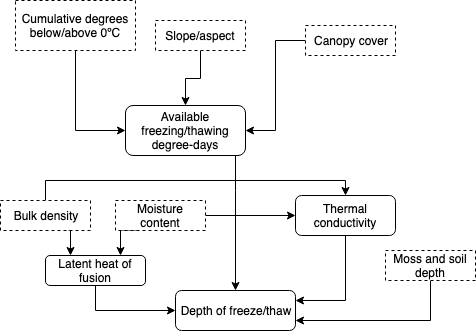
\includegraphics[width=\linewidth]{Figures/Permafrost.png}
  \caption{Flow diagram showing permafrost dynamics simulated in UVAFME.}
  \label{fig:permdiagram}
\end{figure}

The required number of degree-days to thaw a layer of depth $d_s$ (m) is:

\begin{equation}
DD_{req} = Q_ld_s/24\Big(r_{above} + r_s/2\Big)
\end{equation}

where $Q_l$ is the latent heat of fusion of the soil layer (kcal m$^{-3}$), $r_{above}$ is the sum of the thermal resistances of the above soil and moss layers (m$^2$ ºC hr kcal$^{-1}$), and $r_s$ is the thermal resistance of the current soil layer \cite{jumikisThermalSoilMechanics1966, bonanComputerModelSolar1989}. The latent heat of fusion is calculated as:

\begin{equation}
Q_l = (80gw)bd_s
\end{equation}

where $gw$ is soil layer's gravimetric water content ($gw = \frac{1000m_w}{bd_s}$, where $m_w$ is the volumetric moisture content), and $bd_s$ is the bulk density of the soil layer (kg m$^{-3}$) (see Section \ref{soilwater}). The thermal resistance of the soil layer is calculated as $r_s = d_s/k_s$ where $k_s$ is the soil layer's thermal conductivity (kcal m$^{-1}$ hr$^{-1}$ ºC$^{-1}$).

The available degree-days for thawing and freezing (i.e. cumulative monthly degrees above/below 0ºC) are adjusted to account for vegetation cover and light on the forest floor, as well as slope and aspect. Using the canopy openness on the plot, calculated as: $al = \text{e}^{-0.25LAI}$, separate correction factors are determined for freezing ($c_f$) and thawing ($c_t$) degree-days. For $al > 0.75$, $c_t = 0.92$ and $c_f = 0.36$. For $0.50 < al \leq 0.75$, $c_t = 0.77$ and $c_f = 0.37$. For $al \leq 0.50$, $c_t = 0.62$ and $c_f = 0.38$. The topographic correction factor is calculated as: $c_s = R/R_H$ where $R/R_H$ is the ratio of actual surface radiation to horizontal surface radiation (see Section \ref{solar}). The available freezing ($DD_f$) and thawing ($DD_t$) degree-days are then modified as:

\begin{equation}
DD_f = DD_fc_f(2 - c_s)
\end{equation}

and

\begin{equation}
DD_t = DD_tc_tc_s
\end{equation}

Thus, available freezing degree-days decrease with increasing light (i.e. decreasing vegetation cover). The topographic factor acts to decrease available freezing degree-days with sites that have higher actual surface radiation than horizontal surface radiation (i.e. south-facing slopes), and increase freezing degree-days for sites with lower actual surface radiation than horizontal surface radiation (i.e. north-facing slopes). The available thawing degree-days decrease less with increasing available light. The topographic factor acts to increase available thawing degree-days with south-facing slopes, and decreases them for north-facing slopes.

The thermal conductivities of the moss-organic layer and the mineral layer are calculated using the moisture contents, bulk densities, wilting points, and field capacities of the soil layers. As in \citeA{bonanComputerModelSolar1989}, the frozen ($k_f$) and unfrozen ($k_u$) thermal conductivities of the moss-organic layer are calculated as:

\begin{equation}
k_u=\frac{\Big(0.5(m_{pwp}-m_w)+ 0.08(m_w-m_{fc})\Big)}{m_{pwp}-m_{fc}}
\end{equation}

and

\begin{equation}
k_f=\frac{\Big(2.0k_u(m_{pwp}-m_w)+ k_u(m_w-m_{fc})\Big)}{m_{pwp}-m_{fc}}
\end{equation}

where $m_{fc}$ and $m_{pwp}$ are the field capacity and wilting points (volumetric) of the layer. Also as in \citeA{bonanComputerModelSolar1989}, the thermal conductivities for the mineral soil layer (here in Btu in ft$^{-2}$) are calculated using equations from \citeA{lunardiniHeatTransferCold1981}, using separate equations for fine-textured and granular soils:

Fine-textured:

\begin{equation}
k_u = \Big(0.9\log_{10}(100gw) - 0.2\Big) \times 10^{0.01bde_s}
\end{equation}

\begin{equation}
k_f= 0.01 \times 10^{0.022bde_s} + 0.085(100gw) \times 10^{0.008bde_s}
\end{equation}

Granular:

\begin{equation}
k_u = \Big(0.7\log_{10}(100gw) + 0.4\Big) \times 10^{0.01bde_s}
\end{equation}

\begin{equation}
k_f= 0.076 \times 10^{0.013bde_s} + 0.032(100gw) \times 10^{0.0146bde_s}
\end{equation}

where $bde_s$ is the bulk density of the soil in lb ft$^{-3}$. Once the available degree-days and required degree-days for each layer are calculated, the two values are compared. If the available degree-days is greater than or equal to the required degree-days, the depth of freeze/thaw of that layer is set to the entire layer’s depth, and the available degree-days is decremented by that layer’s required degree-days. The model then moves to the lower layer and compares the available degree-days again to the required degree-days.

If the required degree-days is greater than the available degree-days, the available degree-days is set to 0.0, and the depth of freeze/thaw for that layer is calculated using a quadratic formulation:

\begin{equation}
x = \frac{-b + \sqrt{b^2 - 4ac}}{2a}
\end{equation}

where $a = \frac{0.5Q_l}{k_{f,t}}$, $b = Q_lr_{above}$, and $c = -24DD_{f,t}$. Finally, the depths of freeze/thaw for each layer are summed to derive the total depth that day ($d_{melt}$ and $d_{freeze}$). These values are used to update the seasonal maximum depths of freeze ($z_{freeze}$) and thaw ($alt$), and also impact soil water dynamics, decomposition, and plant growth (see Sections \ref{soilwater}, \ref{nutrients}, and \ref{growth}).

\section{Moss} \label{moss}
\numberwithin{equation}{section}

A moss growth and decay subroutine was added to this updated version of UVAFME to calculate the annual growth and decay of moss. As in \citeA{bonanSimulationMossTree1989}, moss growth is modeled as the difference between carbon assimilation and decay/respiration. Due to bryophyte's simple allocation scheme, the relationship between moss photosynthesis and growth/productivity is fairly tight compared to vascular plants \cite{oechelRoleBryophytesNutrient1986}, and thus this relatively simple model of moss growth is appropriate. Carbon assimilation is assumed to be proportional to maximum moss biomass reported for interior Alaska (0.2 kg m$^{-2}$; \citeA{vancleveForestSuccessionRelation1981}), and is modified based on plot conditions such as light level, soil moisture, and litterfall.

\subsection{Moss Growth Factors}

\subsubsection{Light Extinction and Forest Floor Light Conditions}

As in \citeA{bonanSimulationMossTree1989}, a light extinction factor is derived to simulate the effect of light availability on moss photosynthesis. Here, light availability is calculated as:

\begin{equation}
L_{avail} = \text{e}^{-\gamma S_\mu M_{biom}/2}
\end{equation}

where $M_{biom}$ is current moss biomass (kg m$^{-2}$), $S_\mu$ is a specific leaf area parameter, set to 1.7, and $\gamma = 3.5$. Parameter values are taken from Bonan and Korzukhin, where they were derived from data on moss growth from \shortciteA{vancleveProductivityNutrientCycling1983} and \citeA{larcherPhysiologicalPlantEcology1980}. The effect of this light availability on assimilation is then calculated as:

\begin{equation}
f_{ext} = \frac{a_1(L_{avail} - a_3)}{1.0 + a_2L_{avail}}
\end{equation}

where $a_1$ and $a_2$ are light curve parameters, set to 3.41 and 2.14 from \citeA{bonanSimulationMossTree1989}, and $a_3$ is a light compensation point for factor, set to 0.08 from \citeA{bonanSimulationMossTree1989}. A second light factor is calculated to simulate the effect of the forest canopy on moss growth \cite{bonanSimulationMossTree1989}. Increases in canopy openness leads to desiccation of moss and thus this factor decreases with increasing canopy openness above 50\%:

\begin{equation}
f_{can} = \begin{cases}
1.25 - al^2, & \text{$al > 0.5$}.\\
1.0, & \text{$al \leq 0.5$}.
\end{cases}
\end{equation}

where $al = \text{e}^{-0.25LAI}$. To simulate the effect of the forest canopy lowering light availability for moss photosynthesis, another light factor is calculated that increases with increasing canopy  openness below 50\%:

\begin{equation}
f_{shade} = \begin{cases}
b_1 + b_2\sqrt{al}, & \text{$al \leq 0.5$}.\\
1.0, & \text{$al > 0.5$}.
\end{cases}
\end{equation}

where $b_1$ and $b_2$ are parameters, set to 0.8 and 0.8 in this updated version based on moss growth data from  \shortciteA{jeanMurphyDomeMoss2017}. Together, these factors create a parabolic function with moss biomass increasing to a point (50\% cover) and then subsequently decreasing.

\subsubsection{Deciduous Litter and Soil Moisture}
A deciduous litter factor ($f_{decid}$) is calculated to incorporate deciduous litter's inhibition of moss growth and establishment. Using data from \cite{jeanMurphyDomeMoss2017}, this factor is calculated as:

\begin{equation}
f_{decid} = \begin{cases}
1.0 - 75M_{decid}, & \text{$M_{decid} > 0.0$}.\\
1.0, & \text{$M_{decid} = 0.0$}.
\end{cases}
\end{equation}

where $M_{decid}$ is the mass of deciduous leaf litter on the plot (t ha$^{-1}$). As in \citeA{bonanSimulationMossTree1989}, a soil moisture growth factor ($f_{moist}$) is used to simulate desiccation of the moss layer at low moisture levels. If the drought index ($DI$, see Section \ref{growth}) for the year is below 0.10 moss is not allowed to grow. Otherwise, moss is allowed to grow normally:

\begin{equation}
f_{moist} = \begin{cases}
1.0, & \text{$DI \leq 0.10$}.\\
0.0, & \text{$DI > 0.10$}.
\end{cases}
\end{equation}

\subsection{Moss Growth and Decay}

The assimilation rate ($A_r$, kg kg$^{-1}$) is calculated as a function of the maximum moss growth and the previous growth factors:

\begin{equation}
A_r = \mu f_{shade}f_{ext}f_{moist}f_{can}f_{decid}
\end{equation}

where $\mu$ is maximum moss productivity (kg m$^{-1}$). Moss respiration ($R$), is then calculated as a function of moss biomass, deciduous litter, and soil moisture:

\begin{equation}
R = S_\mu M_{biom}(q + b_1) + sf_{moist}f_{decid}
\end{equation}

where $q$, $b_1$, and $s$ are parameters taken from \citeA{bonanSimulationMossTree1989}, set to 0.12, 0.136, and 0.001. Moss growth for the year is then calculated as the difference between assimilation and respiration:

\begin{equation}
P = S_\mu M_{biom}A_r - R
\end{equation}

This value can be positive (for moss growth) or negative (if respiration is greater than assimilation). The growth amount is then added to the current year's biomass. If this value is positive (i.e. moss growth occurred or mortality did not exceed the current biomass), moss biomass is updated to reflect the growth ($M'_{biom} = M_{biom} + P$). If the value is negative, $P$ is set to $-M_{biom}$ and $M'_{biom}$ is then set to 0.0.

Moss litter ($M_{litter}$, kg m$^{-2}$) is calculated as a function of the current year's moss biomass, deciduous litter, soil moisture and growth that year.

\begin{equation}
M_{litter} = S_\mu M_{biom}(A_r - q) + sf_{moist}f_{decid} - P
\end{equation}

This litter amount is added to the set of litter cohorts for decomposition (see Section \ref{nutrients}). The depth of live moss (m) is calculated as $\frac{M'_{biom}}{bd_{moss}plotsize}$, where $plotsize$ is the area of the plot (default to 500 m$^2$ in UVAFME), and $bd_{moss}$ is live moss bulk density, set to a default value of 5.2 kg m$^{-3}$. This moss depth acts to influence permafrost dynamics (see Section \ref{perm} as well as plant regeneration (Section \ref{regen}).

\section{Tree and Shrub Growth} \label{growth}
\numberwithin{equation}{section}

Tree and shrub growth in UVAFME is modeled annually as diameter increment growth, based on first simulating optimal diameter increment growth from \citeA{botkinEcologicalConsequencesComputer1972} and \citeA{leemansFORSKAGeneralForest1989} and subsequently modifying that optimal growth based on environmental conditions and species- and tree/shrub size-specific tolerances \cite{yanFAREASTForestGap2005}. Each year the updated diameter is used to calculate other plant characteristics such as height, leaf area, and biomass using allometric equations.

\subsection{Tree and Shrub Allometry} \label{allometry}

We simulate both trees and shrubs with differing allometry, depending on the growth form of the plant. We use data from \citeA{bernerBiomassAllometryAlder2015} and the Biomass and Allometry Database (BAAD) \cite{falsterBAADBiomassAllometry2015} to develop and parameterize shrub allometric equations.

\begin{figure}
  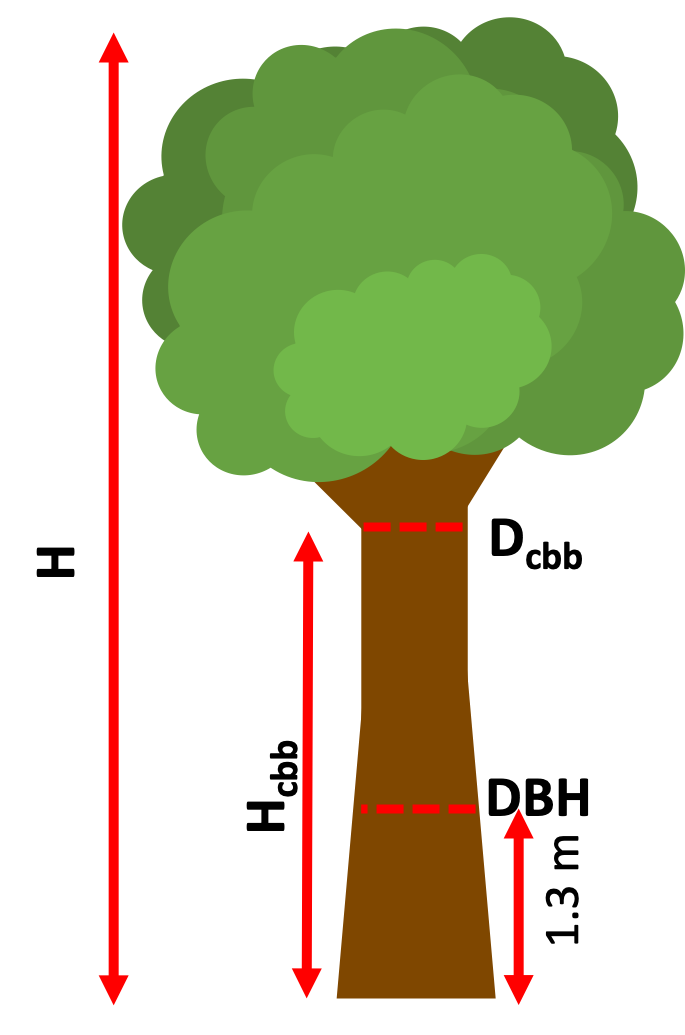
\includegraphics[width=0.5\linewidth]{Figures/Tree_allometry.png}
  \caption{Tree measurements used in tree allometric equations.}
  \label{fig:allometry}
\end{figure}

Optimal diameter growth of a tree ($\delta DBH_{opt_{\text{tree}}}$, cm) is calculated as \cite{botkinEcologicalConsequencesComputer1972}:

\begin{equation} \label{opt}
\delta DBH_{opt_{\text{tree}}} = gDBH\frac{1.0 - \frac{DBH \times H}{DBH_{max}/H_{max}}}{2.0H + sDBH\text{e}^{\frac{-sDBH}{H_{max} - 1.3}}}
\end{equation}

where $H$ is the current tree height (m), $DBH$ is the current diameter at breast height (cm), $H_{max}$ is the species' average maximum height (m), $DBH_{max}$ is the species' average maximum DBH (cm), and $s$ and $g$ are species-specific growth parameters. As in \citeA{botkinEcologicalConsequencesComputer1972}, $g$ is related to the initial rapid rise in diameter of an individual and higher values of $g$ result in faster growth initially (Fig. \ref{fig:optDBH}). The parameter $s$ is the initial slope of the optimal height-diameter relationship of a tree species. 

For non tree-like shrub growth forms, we modify this equation to use basal diameter ($D$, cm), instead of DBH and remove the 1.3 term:

\begin{equation} \label{opt_shrub}
\delta D_{opt_{\text{shrub}}} = gD\frac{1.0 - \frac{D \cdot H}{D_{max}/H_{max}}}{2.0H + sD\text{e}^{\Big(\frac{-sD}{H_{max}}\Big)}}
\end{equation}

\begin{figure}
  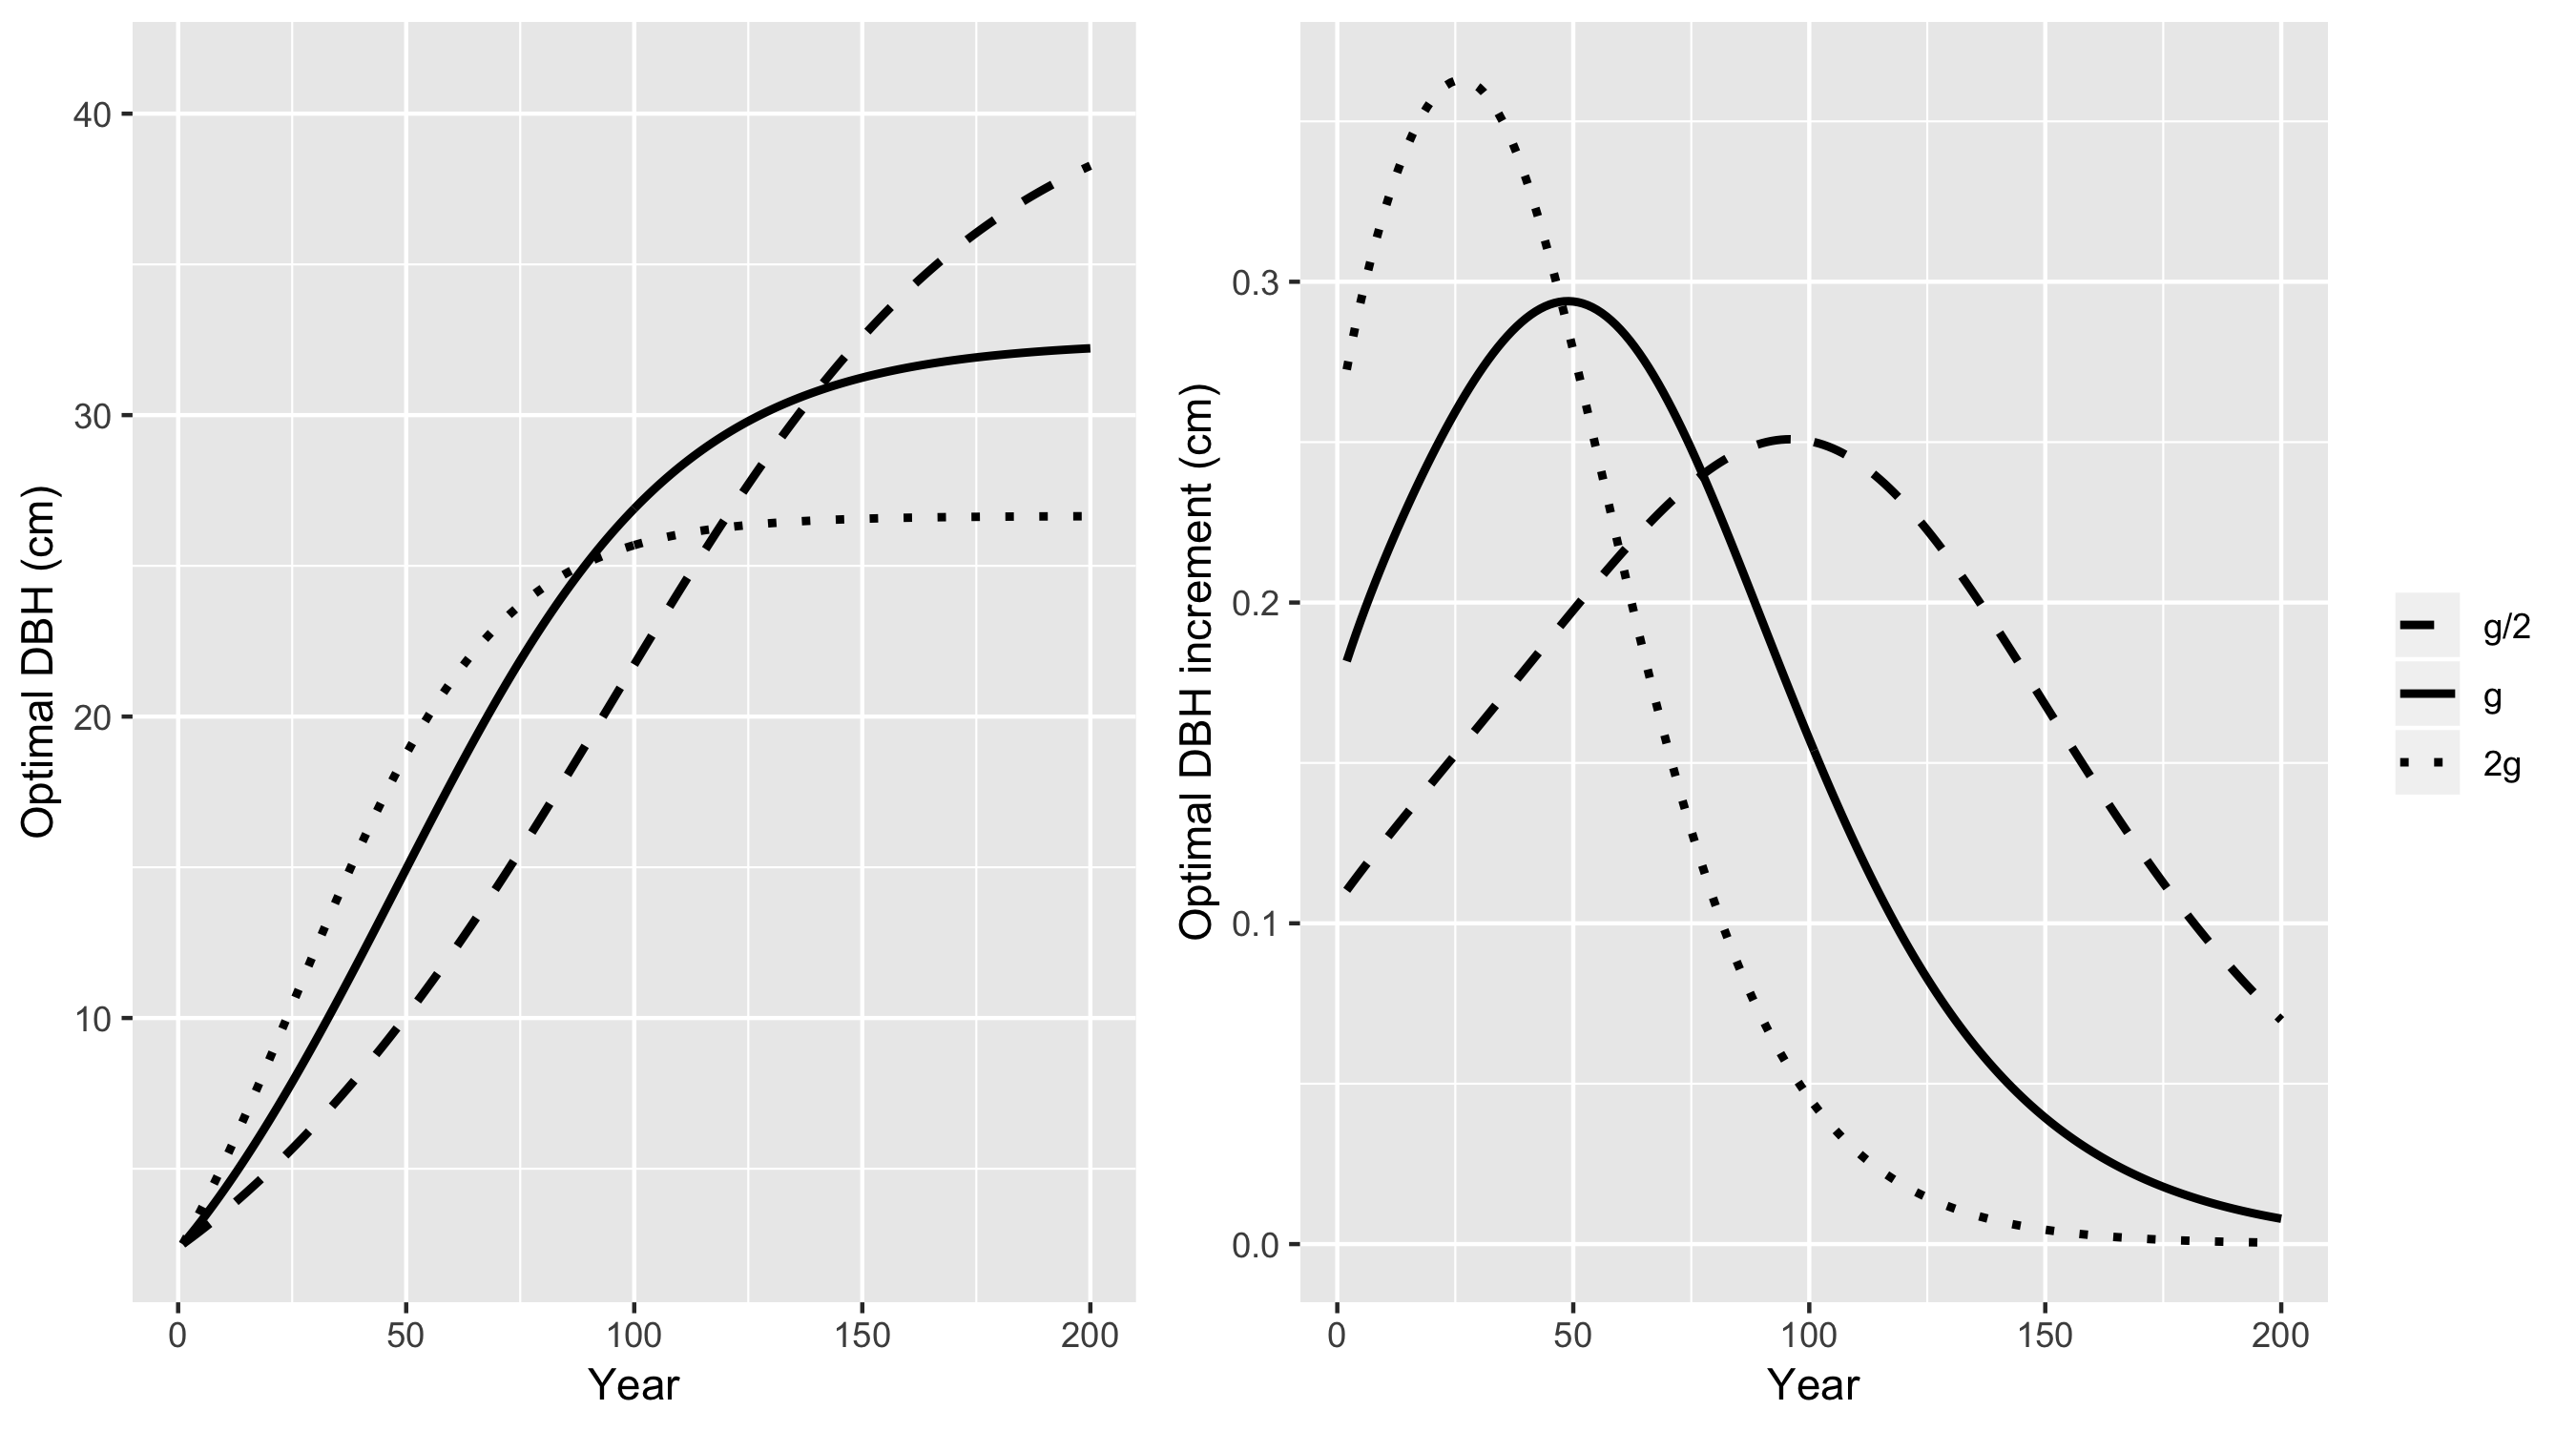
\includegraphics[width=0.9\linewidth]{Figures/optDBH.png}
  \caption{Example calculation of optimal tree diameter over time with changing growth parameter $g$ ($s = 2.02; g = 0.748; H_{max} = 22$ m; $DBH_{max} = 23$ cm; $AGE_{max} = 140$ years) (Eq. \ref{opt}).}
  \label{fig:optDBH}
\end{figure}

Tree height is calculated based on an equation from the FORSKA model \cite{leemansFORSKAGeneralForest1989}.

\begin{equation} \label{height}
H_{\text{tree}} = 1.3 + (H_{max} - 1.3)(1.0 - \text{e}^{-\frac{sDBH}{H_{max} - 1.3}})
\end{equation}

Here, higher values of the input parameter $s$ result in faster  height growth (Fig. \ref{fig:height}).

\begin{figure}
  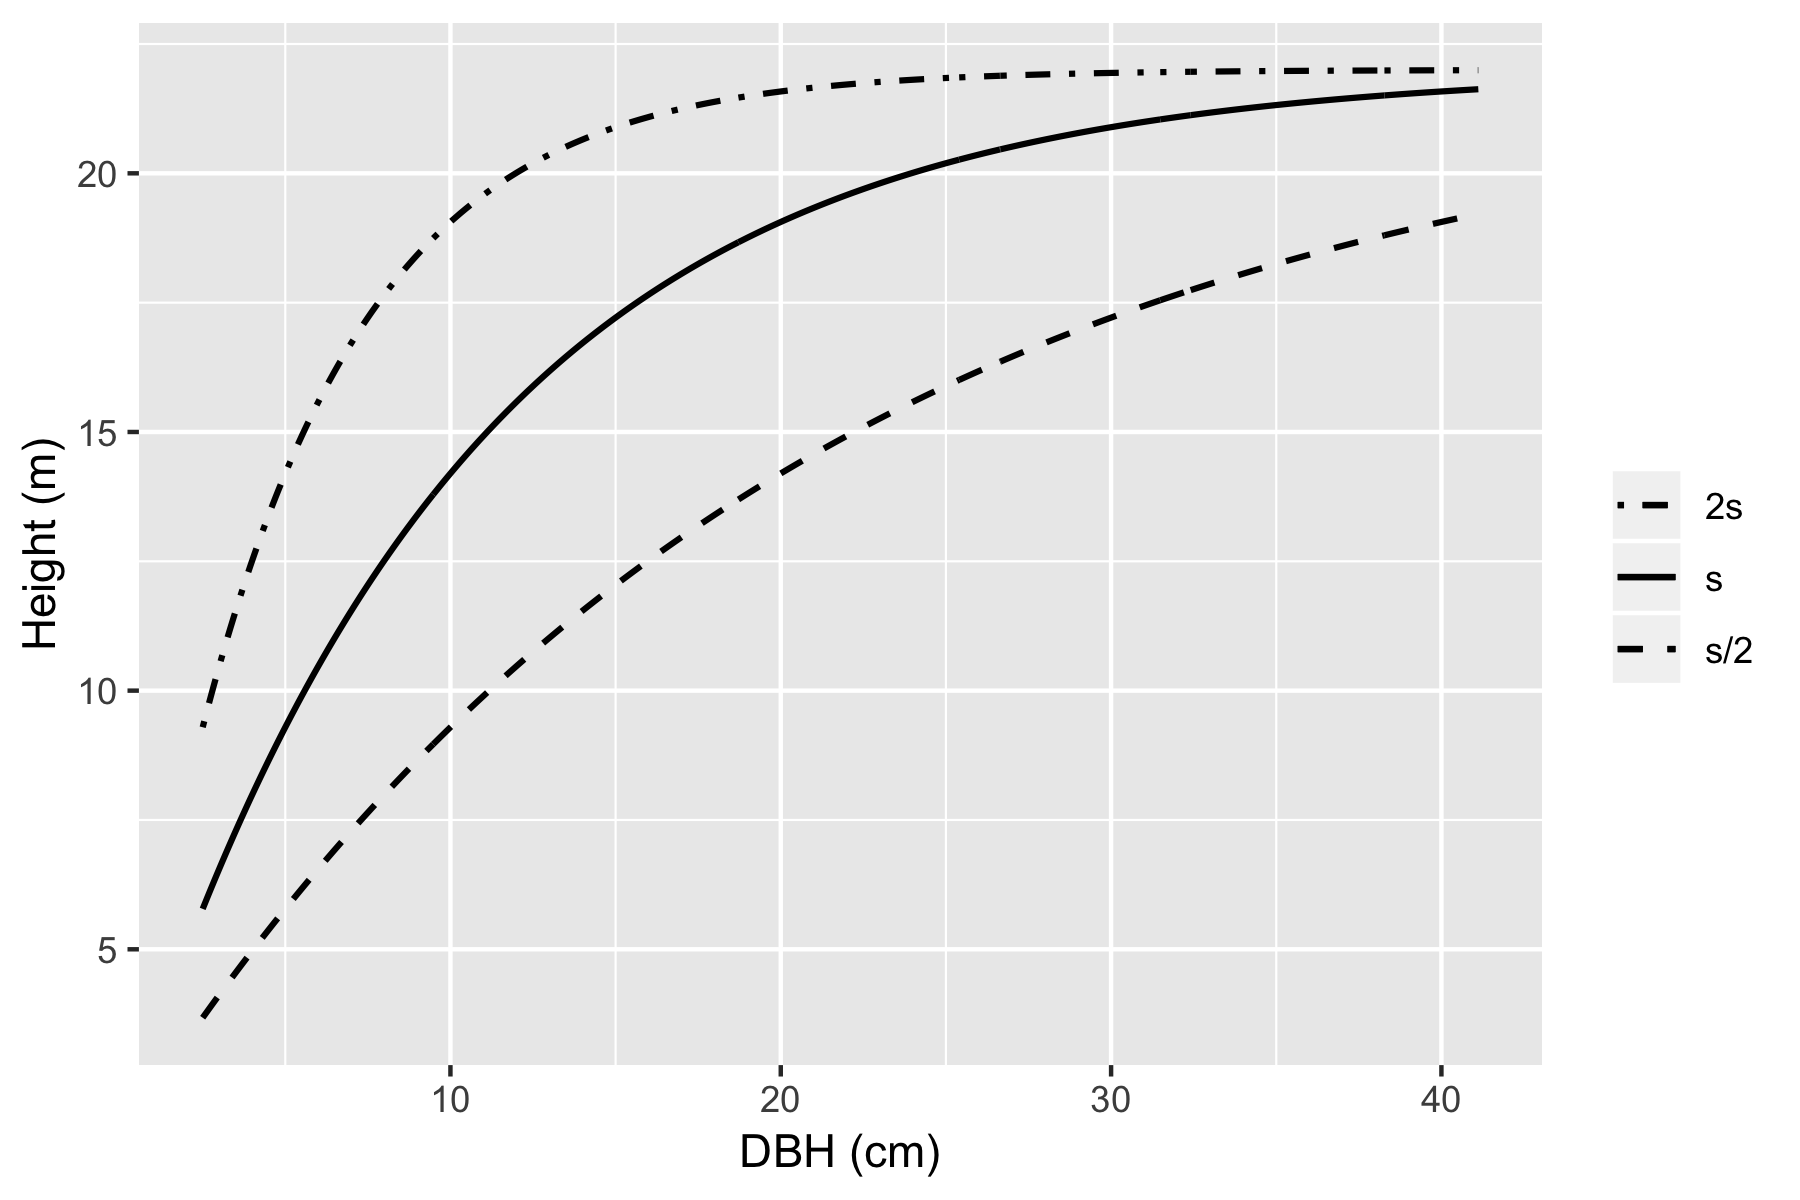
\includegraphics[width=0.9\linewidth]{Figures/height.png}
  \caption{Example calculation of height vs. DBH with changing values of $s$ ($s = 2.02; g = 0.748; H_{max} = 22$ m; $DBH_{max} = 23$ cm; $AGE_{max} = 140$ years) (Eq. \ref{height}).}
  \label{fig:height}
\end{figure}

For shrubs, we use a similar form, but again use basal diameter:

\begin{equation}\label{eq:ht_shrub}
	H_{\text{shrub}} = H_{max}\Bigg(1 - \text{e}^{\Big(-\frac{sD}{H_{max}}\Big)}\Bigg)
\end{equation}

Leaf area of trees ($LA_\text{tree}$, m$^2$) is calculated as a function of the diameter at clear branch bole height, based on the Shinozaki pipe model \shortcite{shinozakiQuantitativeAnalysisPlant1964, yanFAREASTForestGap2005}:

\begin{equation} \label{leafarea}
LA_\text{tree} = D_{cbb}^2D_L
\end{equation}

where $D_{cbb}$ is the diameter at clear branch bole height (cm) (Fig. \ref{fig:allometry}), and $D_L$ is a species input parameter, which ranges from 0.225 to 0.255 depending on species-specific shade tolerance. Diameter at clear branch bole height is calculated assuming a conical bole shape \cite{yanFAREASTForestGap2005}:

\begin{equation} \label{dcbb}
D_{cbb} = \begin{cases}
DBH, & \text{$H \le 1.3$}\\
DBH\Big(\frac{H - H_{cbb}}{H - 1.3}\Big)^{\frac{1}{\beta}}, & \text{$H > 1.3$}
\end{cases}
\end{equation}

where $H_{cbb}$ is clear branch bole height (m) and $\beta$ is a stem shape parameter. In UVAFME, $H_{cbb}$ is not calculated allometrically but set to an initial value (1.0 m) when a tree is first initialized (Section \ref{regen}). It can then increase annually (or not) via lower branch thinning (Section \ref{tgrowth}) \cite{yanFAREASTForestGap2005}. 

Leaf area of shrubs is calculated similarly, but using basal diameter instead of clear branch bole height diameter:

\begin{equation} \label{leafarea_shrub}
	LA_\text{shrub} = D^2D_L
\end{equation}

Wood volume of trees (i.e. biomass) is calculated assuming the bole shape is a simple cone. This volume is then multiplied by the bulk density of the wood (a species-specific input parameter) and divided by 2 to derive biomass in tonnes of C.

\begin{equation}  \label{bbole}
B_{bole} = \Big(\frac{1\times10^{-4}\pi 0.25\rho DBH^2H\beta}{\beta + 2}\Big)0.5
\end{equation}

where $\rho$ is the wood bulk density of the species (tonnes m$^{-3}$). Biomass of branches and the bole above the diameter at clear branch bole height is calculated also assuming the volume is a cone and applying similar scaling factors to derive tonnes C:

\begin{equation}  \label{btwigs}
B_{branch} = \Big[1\times10^{-4}\pi0.25 \rho \Big(\frac{2}{\beta + 2} -0.33\Big)DBH^2H\Big]0.5
\end{equation}

The lateral root volume is assumed to be half of the branch volume, and the root ball volume is calculated by assuming a cone at DBH height downwards to the root depth ($d_{roots}$, m):

\begin{equation}  \label{broots}
B_{roots} = 0.5B_{branch} + B_{bole}\frac{d_{roots}}{H}
\end{equation}

The final total tree woody biomass is derived by summing all parts of the tree ($B_{tree} = B_{bole} + B_{branch} + B_{roots}$). 

Aboveground woody biomass of shrubs ($B_{woody_\text{shrub}}$) is calculated as:

\begin{equation} \label{eq:woodybiom}
	B_{woody_\text{shrub}} = 0.45\frac{(1\times10^{-4}\pi0.25)1.8\rho D^2H\beta}{\beta + 2.0}
\end{equation}

Root biomass of shrubs ($B_{roots_\text{shrub}}$) is calculated as:

\begin{equation} \label{eq:rootbiom_shrub}
	B_{roots_\text{shrub}} = 0.3127B_{woody_\text{shrub}}\frac{d_{roots}}{H}
\end{equation}

Leaf biomass of trees and shrubs is derived using leaf area:

\begin{equation} \label{bleaf}
B_{leaf} = 2.0LMA \times LA
\end{equation}

where $LMA$ is leaf mass per area  (tonnes C m$^{-2}$), set to $5 \times 10^{-5}$ for evergreen and $3.16 \times 10^{-5}$  for deciduous species.

\subsection{Growth Modifiers} \label{gmult}

Annual plant growth is simulated using the above allometric equations for growth, modified by the current environmental conditions on the plot as well as species- and tree/shrub size-specific tolerances. Optimal diameter increment growth (via equation \ref{opt}) is decreased based on soil moisture, temperature, light conditions, nutrient availability, and permafrost conditions (if present). For each of these potential stressors, growth factors are calculated (0 to 1) on a species- and plant-level basis and used to decrease the optimal growth of each plant to derive actual diameter increment growth. For a given plot on a given year, the environmental conditions determine how well each individual plants grows that year. Thus, plants of differing species and sizes will respond differently each year and can compete with one another for resources.

\subsubsection{Temperature}

Plant growth response to temperature is modeled using response to growing degree-days (i.e. cumulative sum of daily temperatures above 5ºC). As in \citeA{fosterValidationApplicationForest2017} and \citeA{shumanFireDisturbanceClimate2017}, temperature response is modeled as an asymptotic increase with increasing growing degree-days, depending on species-specific growing degree-day tolerances. This asymptotic growth response does not penalize species' growth at or above it's optimum growing degree-days, but does restrict growth below this value, with no growth occurring below a species' minimum growing degree-days.

\begin{equation} \label{tempF}
f_{gdd} = 
\begin{cases}
0.0, & \text{$GDD \leq GDD_{min}$}\\
{\frac{GDD - GDD_{min}}{GDD_{opt} - GDD_{min}}^a}{\frac{GDD_{max} - GDD}{GDD_{max} - GDD_{opt}}}^b, & \text{$GDD_{min} < GDD < GDD_{opt}$}\\
1.0, & \text{$GDD \geq GDD_{opt}$}
\end{cases}
\end{equation}

where $a = \frac{GDD_{opt} - GDD_{min}}{GDD_{max} - GDD_{min}}$, $b = \frac{GDD_{max} - GDD_{opt}}{GDD_{max} - GDD_{min}}$, and $GDD_{min}$, $GDD_{opt}$, and $GDD_{max}$, are the minimum, optimum, and maximum growing degree-days for a species.

\begin{figure}
  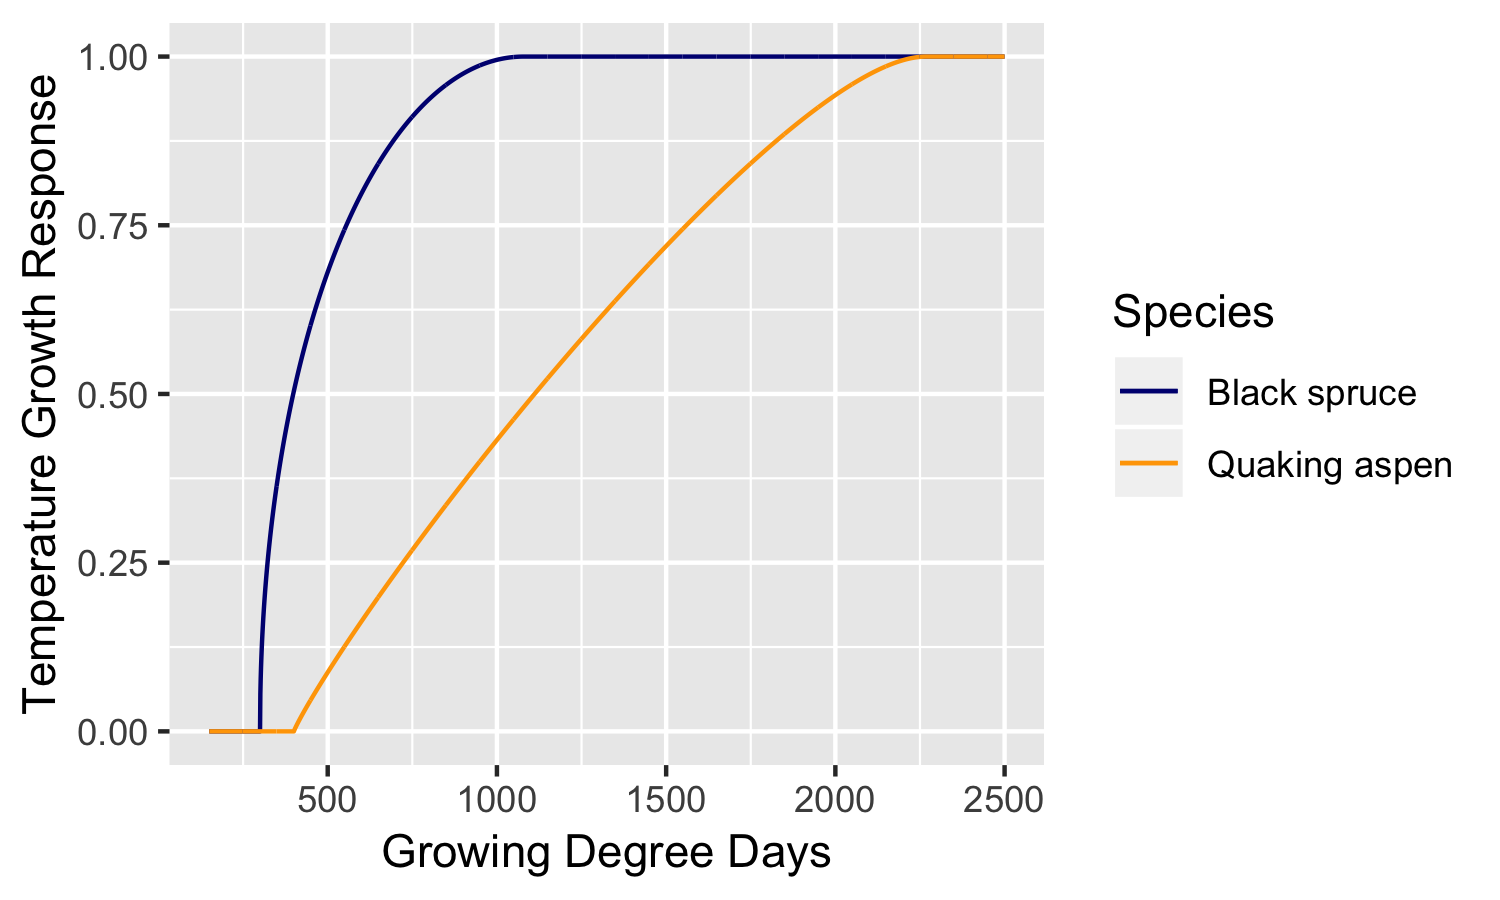
\includegraphics[width=0.9\linewidth]{Figures/tempResp.png}
  \caption{Example species growth response to growing degree-days. Black spruce: $GDD_{min} = 300$, $GDD_{opt} = 1079$, $GDD_{max} = 1911$. Aspen: $GDD_{min} = 400$, $GDD_{opt} = 2268$, $GDD_{max} = 2461$.  (Eq. \ref{tempF}).}
  \label{fig:temp}
\end{figure}

\subsubsection{Soil Moisture}
The growth factor for moisture availability is calculated based on soil moisture conditions throughout the year as well as the ratio of precipitation to PET and AET to PET. Using the daily simulation of soil moisture (section \ref{soilwater}), indices are derived that relate a single day's soil moisture to the field capacity and wilting point of the soil. Two drought indices (ranging from 0 to 1) are utilized: $DI_u$ and $DI_b$. $DI_u$ represents the proportion of the growing season where $SW_{FC} < 0.75$, where $SW_{FC} = \frac{w_{l_{min}}}{m_{FC_{min}}}$. Here, $w_{l_{min}}$ is mineral layer liquid water content (m) and $m_{fc_{min}}$ is mineral layer field capacity (m). $DI_b$ is represents the percent of the growing season where $SW_{WP} < 1.2$, where $SW_{WP} = \frac{w_{l_{min}}}{m_{pwp_{min}}}$. Here $m_{pwp_{min}}$ is mineral layer wilting point (m). The growing season is defined as the part of the year where the average daily temperature is above 5ºC.

$DI_u$ is further modified as the average of $DI_u$ and $DI_{clim}$, where 

\begin{equation}
DI_{clim} = 1.0 -  \max\Bigg(\min\Big(\frac{P}{PET}, 1.0\Big), \min\Big(\frac{AET}{PET}, 1.0\Big)\Bigg)
\end{equation}

These drought indices are used to calculate an annual drought growth factor (ranging from 0 to 1, with 0 indicating soil moisture as completely limiting to growth, and 1 indicating no effect of soil moisture on growth) based on species-specific drought tolerance. 

\begin{equation} \label{drf}
f_{drought} = \sqrt{\frac{ \max(k_{dry} - DI, 0.0)}{k_{dry}}}
\end{equation}

where $k_{dry}$ ranges from 0.50 to 0.01 depending on species drought tolerance. Input species-level drought tolerance ranges from 1 to 6, with 1 being the most tolerant, and 6 being the least tolerant. For species with a tolerance level of 1 (i.e. very tolerant), $DI = DI_b$, whereas for all other species $DI = DI_u$. For very tolerant species, $f_{drought}$ is further modified as the maximum (i.e. least limiting) of $b(f_{drought})$ and $f_{drought}$ calculated as above but using $DI = DI_u$, where $b = 0.33$ for evergreen species and $b = 0.2$ for deciduous species. This allows for the most tolerant species to have an extra advantage with regards to soil moisture availability (Fig. \ref{fig:drought}).

\begin{figure}
  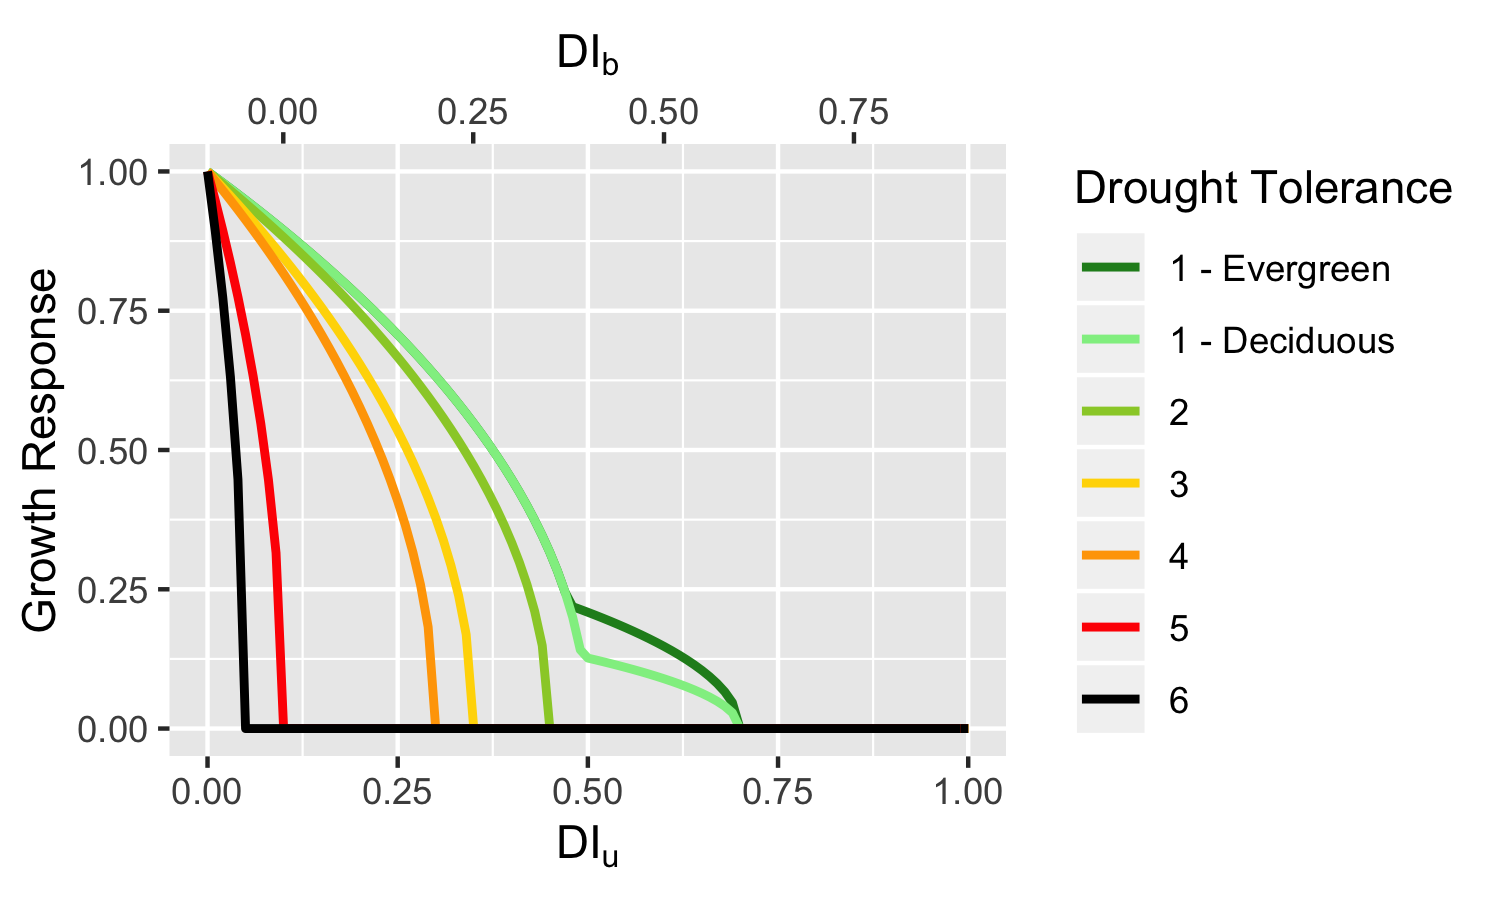
\includegraphics[width=0.9\linewidth]{Figures/drought.png}
  \caption{Species growth response to drought indices. $DI_b$ is used for species with high tolerance (1). $DI_u$ is used for all other species (Eq. \ref{drf}).}
  \label{fig:drought}
\end{figure}

\subsubsection{Light and Shading}

Plant growth response to shading is modeled using available light, calculated according to the vertical distribution of leaf area (Eq. \ref{leafarea}) on the plot. The canopy subroutine is used to calculate this vertical distribution of leaf area. This subroutine uses the leaf area from each tree/shrub on each plot to calculate an overall plot-level cumulative leaf area, distributed vertically depending on the heights of the plants on the plot (Fig. \ref{leafarea}). Shrub species that are of a ``prostrate" form (e.g. \textit{Betula glandulosa}), do not extend vertically into the canopy beyond 1 m in height. These individuals may grow in stem length, but do not contribute to canopy biomass or shading above 1 m.


\begin{figure}
  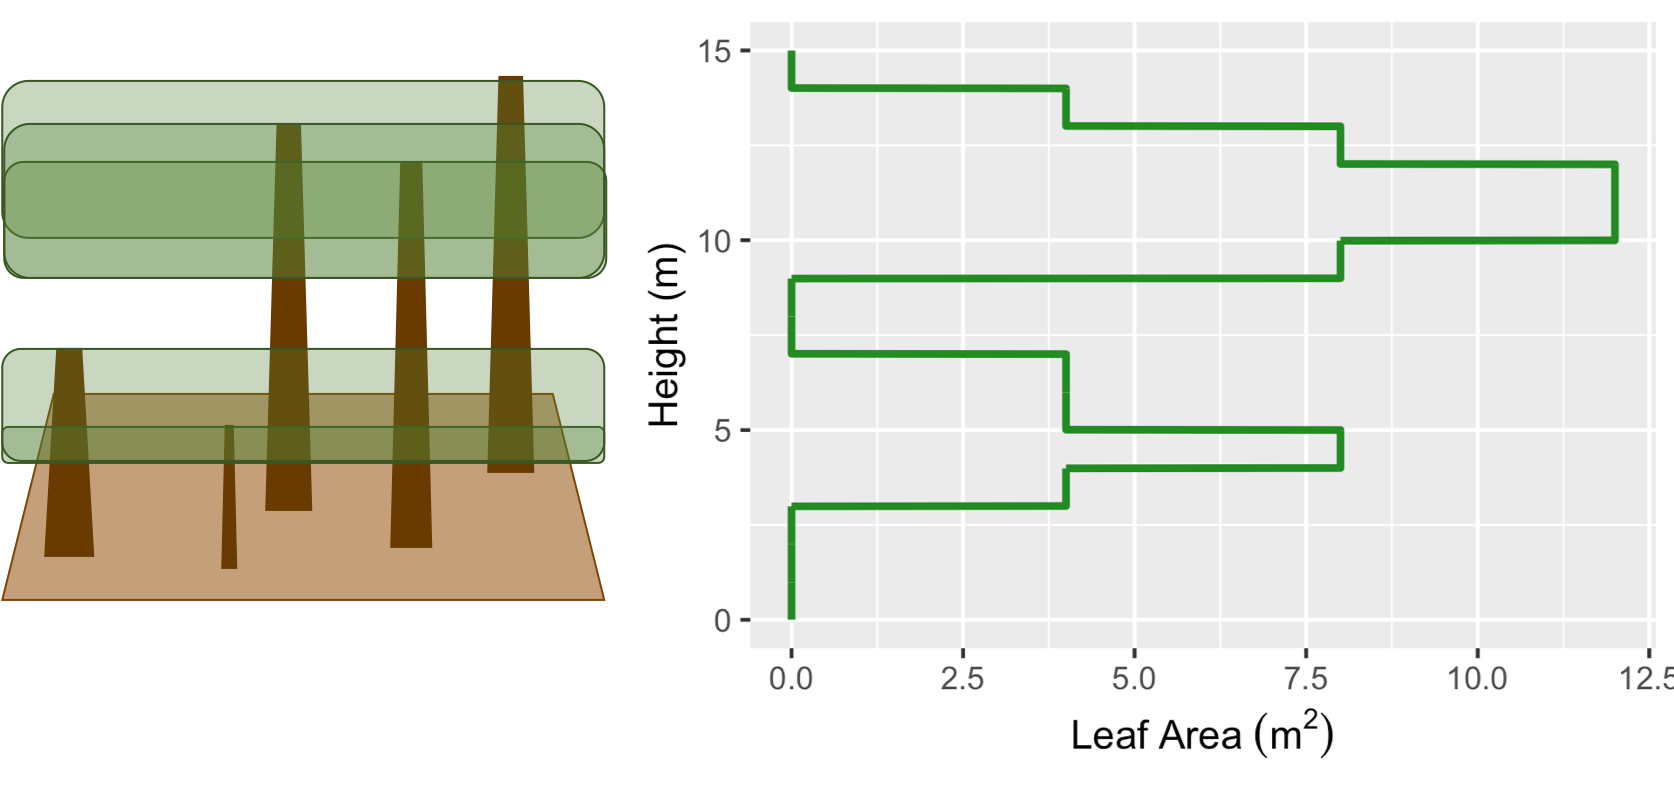
\includegraphics[width=0.9\linewidth]{Figures/Forest_LeafARea.png}
  \caption{Example of vertically distributed leaf area of a plot in UVAFME. Forest canopies are assumed to be horizontally homogenous within a plot.}
  \label{fig:leafarea}
\end{figure}

\begin{figure}[H]
  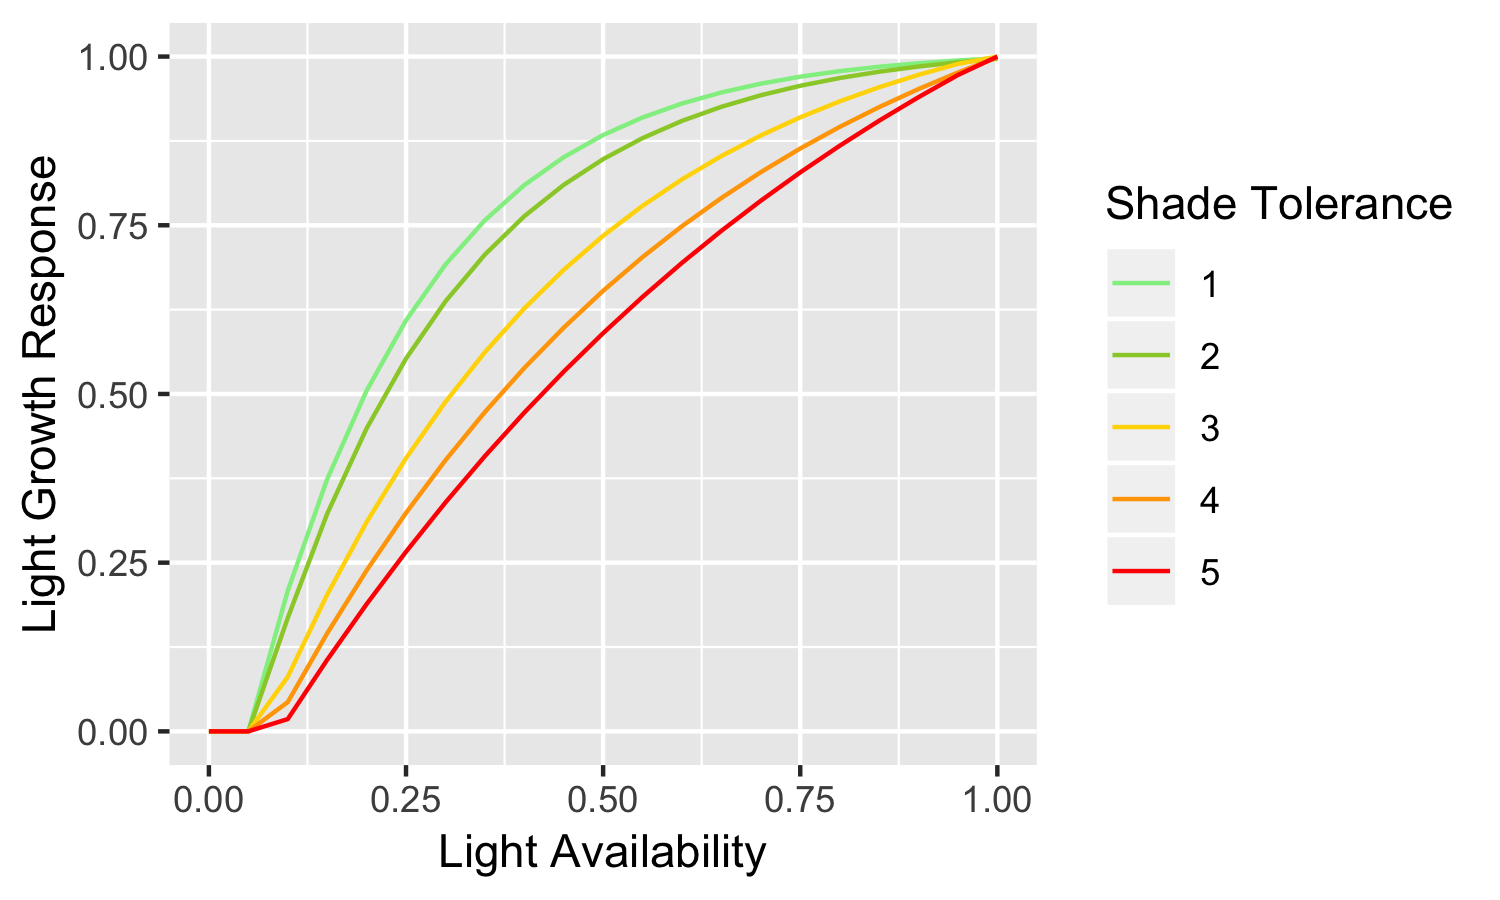
\includegraphics[width=0.9\linewidth]{Figures/lightResp.png}
    \caption{Species growth response to light availability (Eq. \ref{lightf}). A shade tolerance of 1 corresponds to very shade tolerant, a shade tolerance of 5 corresponds to very intolerant.}
  \label{fig:flight}
\end{figure}

This height-structured leaf area is then used to determine light extinction through each 1-meter layer in the canopy. Deciduous leaf area experienced by evergreen species is reduced by 80\% to account for the part of the year without deciduous leaf cover. This reduced leaf area results in a higher light environment for evergreen species relative to deciduous species. Light availability in the $i$th layer is calculated via the Beer-Lambert law:

\begin{equation} \label{beerlaw}
L_i = \text{e}^{-cLAI_{i+1}}
\end{equation}

where $c$ is an extinction coefficient, set to 0.40, and $LAI_{i+1}$ is the cumulative leaf area index (i.e. cumulative leaf area divided by plotsize, m m$^{-1}$) of the layer above the $i$th layer.

The plant growth response to light availability is calculated as:

\begin{equation} \label{lightf}
f_{light} = k_{l1}(1.0 - \text{e}^{-k_{l2}(L_h - k_{l3})})
\end{equation}

where $k_{l1}$, $k_{l2}$, and $k_{l3}$ depend on species-specific shade tolerance (1 through 5, 5 being least tolerant), and $L_h$ is the light availability at the plant's height (Fig. \ref{fig:flight}).

\subsubsection{Nitrogen Availability}

\begin{figure}[H]
  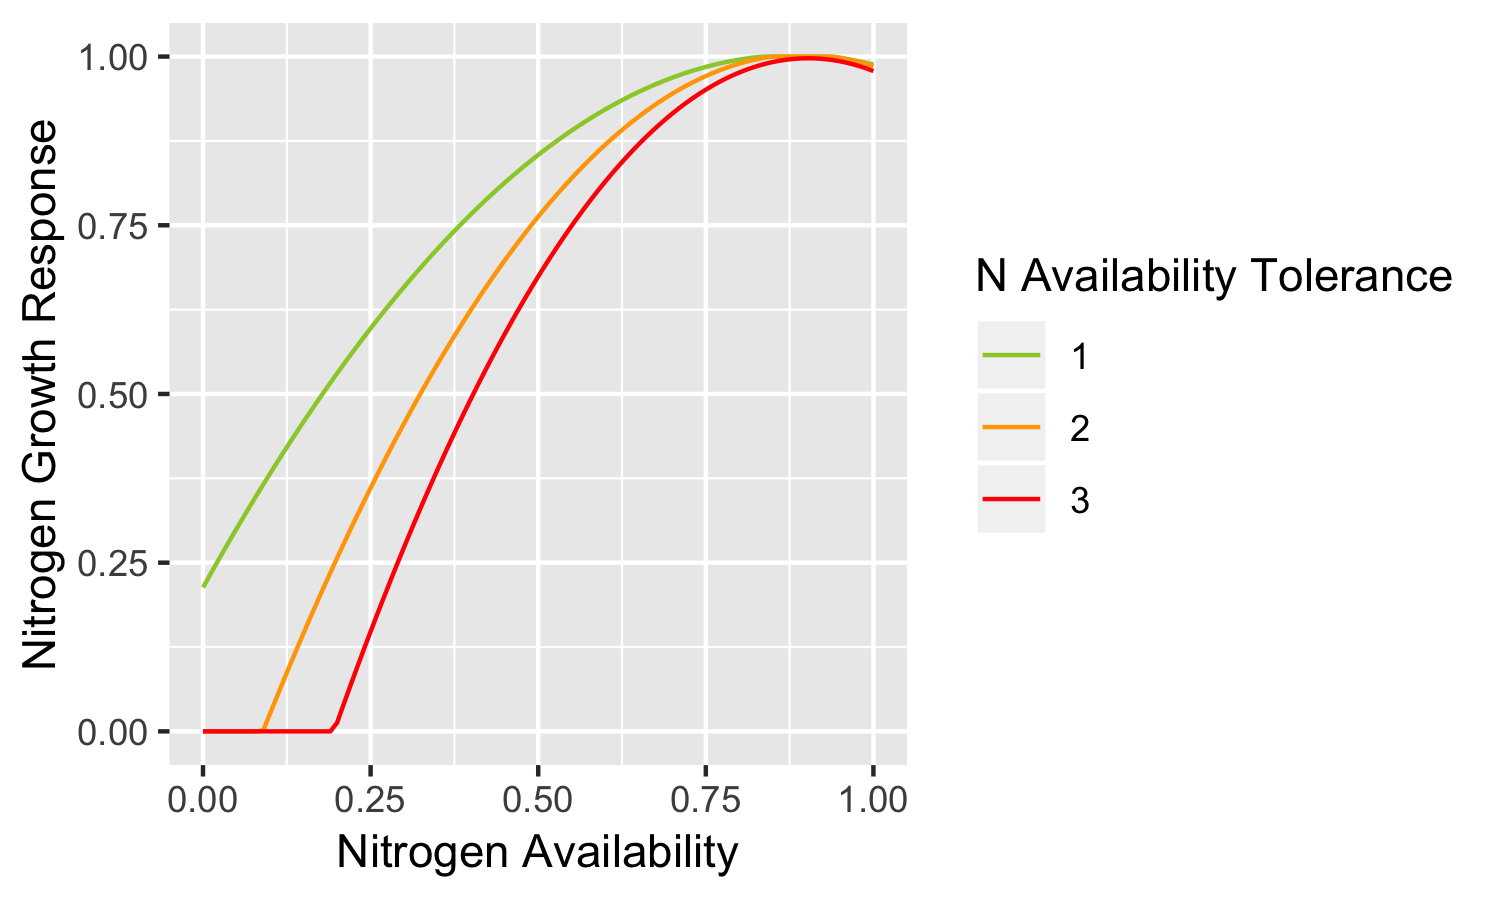
\includegraphics[width=0.9\linewidth]{Figures/fertResp.png}
  \caption{Species growth response to N availability (Eq. \ref{Nf}). A nitrogen tolerance of 1 corresponds to very tolerant, a nitrogen tolerance of 3 corresponds to very intolerant.}
  \label{fig:fpoor}
\end{figure}

Growth response to nitrogen availability is modeled in response to a relative N availability variable, calculated using the ratio of available N to required N. Available N is calculated in the soil decomposition subroutine (Section \ref{nutrients}). Required N is calculated by determining the actual diameter increment growth using all growth modifiers except N availability and then calculating the amount of N required for that potential growth (see Section \ref{tgrowth}). 

The plant growth response to this availability ratio is:

\begin{equation} \label{Nf}
f_{N} = k_{N1} + k_{N2}N_r + k_{N3}N_r^2
\end{equation}

where $k_{N1}$, $k_{N2}$, and $k_{N3}$ depend on species-specific nutrient availability tolerance (1 to 3, 3 being least tolerant), and $N_r$ is the ratio of available N to required N (Fig \ref{fig:fpoor}).


\subsubsection{Permafrost}

If permafrost is present, optimal plant growth is also decreased based on active layer depth (see Section \ref{perm}) and species-specific permafrost tolerance ($tol_{perm}$, 1: tolerant, 2: intolerant). Plant growth response to permafrost presence is based on equations from Bonan (1989) (Fig. \ref{fig:permff}):

\begin{equation} \label{permf}
f_{perm} = \begin{cases}
1.28alt, & \text{$alt \leq 0.6$ and $tol_{perm} = 1$}\\
0.494alt, & \text{$alt \leq 0.6$ and $tol_{perm} = 2$}\\
1.0, & \text{$0.6 < alt \leq 1.0$ and $tol_{perm} = 1$}\\
0.8alt, & \text{$0.6 < alt \leq 1.0$ and $tol_{perm} = 2$}\\
1.0, & \text{$alt > 1.0$}\\
\end{cases}
\end{equation}

where $alt$ is active layer thickness (m).

\begin{figure}
  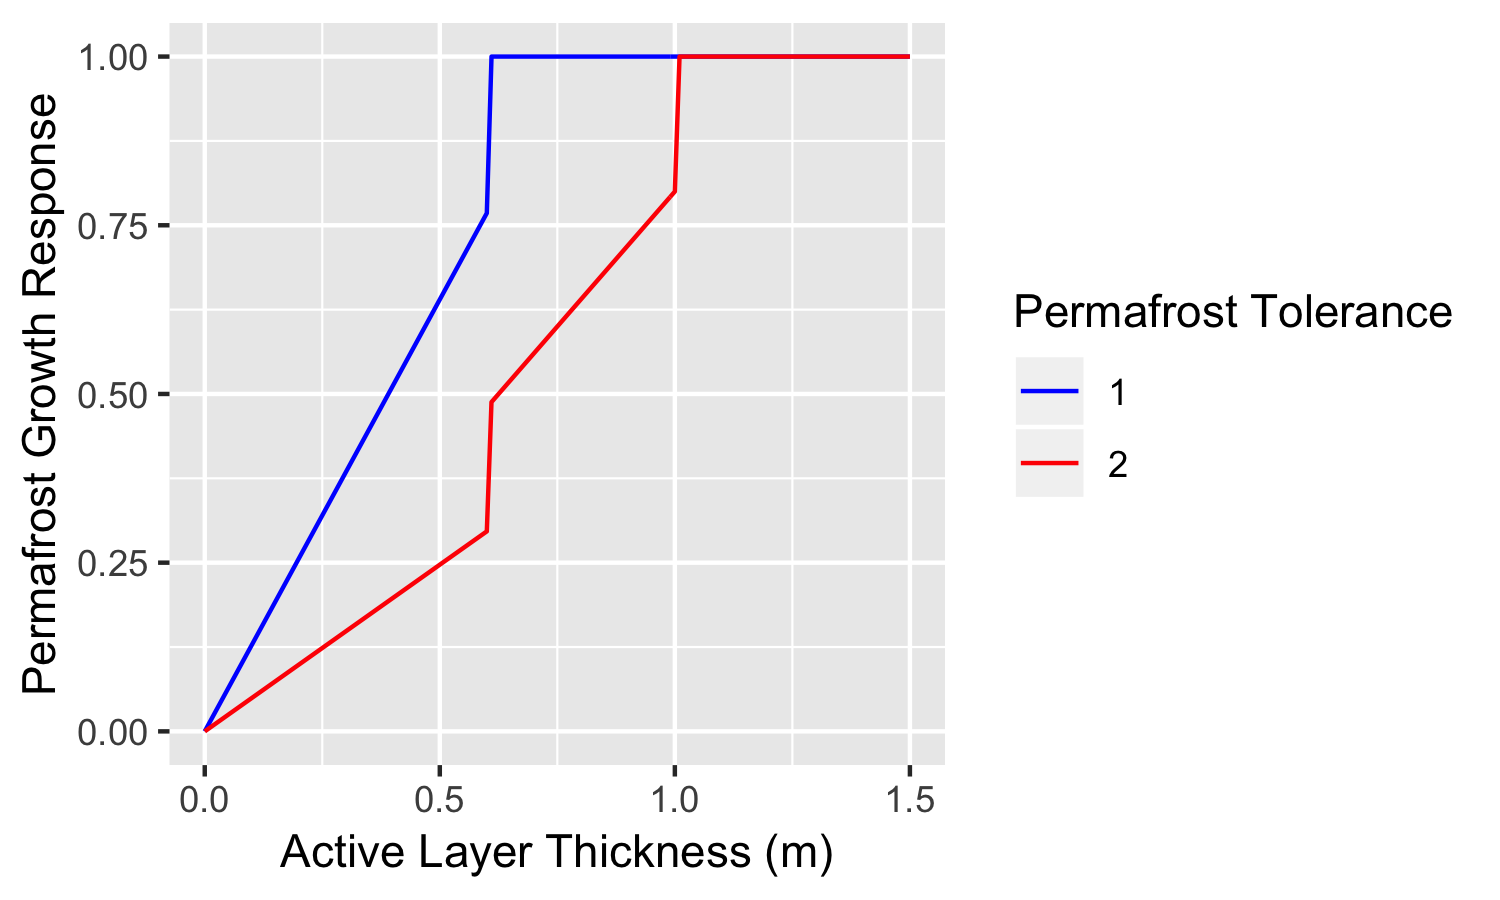
\includegraphics[width=0.9\linewidth]{Figures/permf.png}
  \caption{Species growth response to active layer depth (Eq. \ref{permf}) for tolerant (1) and intolerant (2) species.}
  \label{fig:permff}
\end{figure}

\subsubsection{Inundation}

 Limitation from inundation (i.e. a water table close to the surface) is simulated using equations from \citeA{botkinForestDynamicsEcological1993}. The effect of inundation on vegetation growth is calculated as:

\begin{equation} 
	f_{inun} = \sqrt{\frac{\text{max}(\gamma - ID, 0.0)}{\gamma}}
\end{equation}

where $ID$ is a inundation index, indicating the proportion of the growing season with inundated conditions, and $\gamma$ is a species-specific parameter ranging from 0.99 for very tolerant species to 0.1 for very intolerant species. The inundation index is calculated as the proportion of the growing season where $\frac{m_A}{m_{SAT_A}} > 0.8$, where $m_A$ is the soil moisture (m$^3$ m$^{-3}$) of the mineral layer, and $m_{SAT_A}$ is the saturation capacity (m$^3$ m$^{-3}$) of the mineral layer. As with other growth factors, the inundation factor ($f_{inun}$) is multiplied by the optimal diameter increment growth to obtain actual diameter increment growth (see \citeA{fosterImportanceTreeSpecieslevel2019}), and is also multiplied by other growth factors to reduce species-specific regeneration capacity.

\subsection{Annual Growth} \label{tgrowth}

Annual plant growth is modeled based on first calculating optimal diameter increment growth (Eq. \ref{opt}), and then decreasing that growth based on soil moisture, light availability, temperature, and permafrost (if present). This version of UVAFME uses Liebig's Law of the Minimum (as in \citeA{pastorDevelopmentLinkedForest1985}) to decrease growth, assuming that plants are only growth limited by their most limiting stressor (apart from permafrost, which is used as a multiplicative factor):

\begin{equation} 
\delta D'_{actual} = \delta D_{opt}f_{perm}f_{inun} \times \min(f_{gdd}, f_{drought}, f_{light})
\end{equation}

where $\delta D'_{actual}$ and $ \delta D_{opt}$ are the actual and optimal diameter growth (cm) of the tree (DBH) or shrub (basal diameter, respectively). Here the effect of N availability on plant growth is not yet incorporated into the intermediate value of DBH growth. This intermediate $\delta D'_{actual}$ is used to calculate intermediate values of height ($H'$, Eq. \ref{height}), diameter at clear branch bole height ($D'_{cbb}$, Eq. \ref{dcbb}), leaf biomass ($B'_{leaf}$, Eq. \ref{bleaf}), and woody biomass ($B'_{plant}$, Eq. \ref{bbole} - \ref{broots}). The amount of N required ($N_{req}$, tonnes N) for this potential growth is then calculated as:

\begin{equation} \label{Nreq}
N_{req} = \begin{cases}\!
\begin{aligned}
& (b_lB'_{leaf} - B_{leaf})/CN_{ev} + \\
& (B'_{plant} - B_{plant})/CN_{stem}, \end{aligned} & \text{\footnotesize{evergreen species}} \\
B'_{leaf}/CN_{dec} + (B'_{plant} - B_{plant})/CN_{stem}, & \text{\footnotesize{deciduous species}} 
\end{cases}
\end{equation}

where $b_l$ a conifer:deciduous leaf ratio parameter, set to 1.3, $B'_{leaf}$ is the intermediate value for leaf biomass before calculating N limitation (tonnes C), $B_{leaf}$ is the current leaf biomass (prior to this year's growth), $CN_{ev}$ and $CN_{dec}$ are the C:N ratios of evergreen and deciduous species, set to 60 and 40, respectively, $B'_{plant}$ is the intermediate value for woody biomass, $B_{plant}$ is the current woody biomass, and $CN_{stem}$ is the C:N ratio of woody material, set to 450. The required N is then used to calculate an N availability ratio:

\begin{equation} \label{Nr}
N_r = N_{avail}/\Big(\frac{10000N_{req}}{plotsize}\Big)
\end{equation}

where $N_{avail}$ is plant-available N (tonnes N ha$^{-1}$, see Section \ref{nutrients}), and $plotsize$ is the plot area (in m$^2$). This N availability ratio is used to calculate plant growth response to N availability as in Equation \ref{Nf}. The new actual diameter increment growth is then calculated as:

\begin{equation} 
\delta D'_{actual} = \delta D_{opt}f_{perm}f_{inun} \times \min(f_{gdd}, f_{drought}, f_{light})
\end{equation}

The updated plant diameter is then used to calculate new values for plant height ($H$), diameter at clear branch bole height ($D_{cbb}$), leaf biomass ($B_{leaf}$), and stem C and N weights ($B_{plant}$, $B_{Nplant}$). The amount of N in the plant is calculated as $B_{plant}/CN_{stem}$. The  amount of N used in plant growth this year is calculated as:

\begin{equation} \label{Nused}
N_{used} = \begin{cases}
\begin{aligned}
& \delta B_{plant}/CN_{stem} + \\
& (b_lB'_{leaf} - B_{leaf})/CN_{ev}, \end{aligned}  & \text{for evergreen species} \\
\delta B_{plant}/CN_{stem} + B_{leaf}/CN_{dec}, & \text{for deciduous species}
\end{cases}
\end{equation}

where $\delta B_{plant}$ is the difference between the previous year's stem biomass and this year's stem biomass (tonnes C).

The actual diameter increment growth is also used to check for growth stress-related mortality. A plant has a potential for mortality given two checks: (1) The actual diameter increment growth is checked against a minimum diameter growth parameter, $c_{g}$ (Eq. \ref{cage}), and (2) the growth delimiter (i.e. $f_{lim} = f_{perm}\min(f_{gdd}, f_{drought}, f_{light}, f_N)$) is checked against a minimum growth threshold, $\delta DBH_{min}$, set to a default value of 0.03 cm.

\begin{equation} \label{cage}
c_{g} = \min\Big(\frac{D_{max}}{0.1AGE_{max}}, \delta D_{min}\Big)
\end{equation}

If $\delta D_{actual} \leq c_{g}$ or if $f_{lim} \leq \delta D_{min}$ then the plant's mortality counter ($m_{count}$) is increased by 1.  If this value reaches 2 (i.e. if the plant experiences low growth or stressful conditions for 2 consecutive years), the plant is flagged for potential growth stress-related mortality (Section \ref{stress}). Otherwise, $m_{count}$ is (re)set to 0 and no stress flag is added.

The N used by plant growth on the plot is subtracted from the overall available N (tonnes N ha$^{-1}$; $N_{avail} = \max(N_{avail} - \frac{10000}{plotsize}N_{used}, 0.0)$, where $plotsize$ is plot area in m$^2$) and used in the regeneration subroutine (Section \ref{regen}) to determine whether and how many new plants may be established.

\subsubsection{Lower Branch Thinning} \label{thinning}

UVAFME also checks for stress-induced lower branch thinning, which would increase the clear branch bole height ($H_{cbb}$). If $f_{lim} \leq \delta DBH_{min}$, then lower branch thinning occurs via an increase in $H_{cbb}$ at a rate of 1.01 m in height. $H_{cbb}$ is increased by 1.01 m (checking first to make sure this would not cause $H_{cbb} > H$), and then updated values for $D_{cbb}$ and $B_{plant}$ are calculated. 

The litterfall from this branch thinning is added to the appropriate litter cohort pools (i.e. genus-specific leaf litter, and twig, stem, and root litter; Section \ref{nutrients}). 

\section{Mortality} \label{mortality}
\numberwithin{equation}{section}
Trees and shrubs in UVAFME may die from stress- or age-related factors (Section \ref{tgrowth}) or from disturbances by wildfire, windthrow, and bark beetles \cite{fosterModelingInteractiveEffects2018, shumanFireDisturbanceClimate2017, fosterValidationApplicationForest2017}. Currently, fire and windthrow occurrence are probabilistic, based on site-specific input mean return intervals. If no fire or windthrow disturbance occurs on the plot, only mortality from low growth, age, or insect infestation is considered. 

\subsection{Growth Stress or Age} \label{stress}

\subsubsection{Stress}
Plants that had a potential mortality flag from prolonged low growth or stress (Section \ref{tgrowth}) are checked for stress-related mortality via an input species-specific stress tolerance parameter. A uniform random number between 0 and 1 (see Section \ref{random}) is generated and checked against $c_{stress}$, which ranges from 0.21 to 0.33 depending on the input stress tolerance (1-5; 1: high tolerance, 5: low tolerance). If the random number is below $c_{stress}$ then the plant is set to die from low growth.

\subsubsection{Age}
Plants also have a chance of dying each year based on the input species-specific probability of reaching its maximum age. Again, a random uniform number between 0 and 1 is checked against a parameter, $p_{mage} =1 - \text{e}^{-k_{age}/AGE_{max}}$, where $k_{age}$ is a parameter equalling 4.605, 6.908, or 11.51, depending on the species-specific age parameter (1-3; 1: high probability of reaching $AGE_{max}$, 3: low probability of reaching $AGE_{max}$). These parameters are based on a plant having a 1\%, 0.1\%, and 0.0001\% chance of reaching the plant species' average maximum age \cite{shugartModelingForestLandscapes1985, botkinEcologicalConsequencesComputer1972}.

 If the random number is below $p_{mage}$ then the individual is set to die from random mortality. It is important to note that $p_{mage}$ does not change with individual plant age, but is only related to the species' average maximum age and its probability of reaching that age. 

\subsubsection{Litter}
Trees and shrubs that die and the associated litter is placed in appropriate litter cohorts for decomposition (Section \ref{nutrients}). Leaf litter biomass ($B_{leaf}/c$, $c = 0.45$, tonnes) is added to a genus-specific annual litter pool, $M_{gen}$. Twig litter ($B_{twigs}/c$) is added to a twig litter ($M_{twigs}$, tonnes) pool, and root litter ($B_{roots}/c$) is added to a root litter pool ($M_{roots}$, tonnes). If the plants's diameter is below 10 cm, the stem biomass ($B_{bole}/c$) is added to a small wood litter pools ($M_{Swood}$, tonnes), otherwise it is added to a large wood litter pool ($M_{Lwood}$, tonnes). 

If the plant does not die, the amount of annual litter is calculated as: 

\begin{equation} \label{annlit}
M_{leaves} = \begin{cases}
B_{leaf}(1 - b_l)/c, & \text{for evergreen species} \\
B_{leaf}, & \text{for deciduous species} 
\end{cases}
\end{equation}

where $b_l$ is a coniferous leaf area ratio parameter, set to 1.3.

\subsection{Fire Disturbance} \label{disturbances}
 
As of version 3 \cite{foster_bottom-up_2022}, we represent interactions between fuels, fire weather, climate, and fire mortality and post-fire regrowth. These updates are based on equations from \citeA{rothermelMathematicalModelPredicting1972}, \citeA{thonickeInfluenceVegetationFire2010}, and others.

\subsubsection{Fuel Characteristics}

Fuel characteristics are calculated based on input litter from the plant growth and mortality routines \cite{fosterImportanceTreeSpecieslevel2019}. Litter input from leaf senescence, lower branch thinning, and mortality are added annually to decaying litter type-specific cohorts. These cohorts decay in response to litter characteristics (e.g. N and lignin content) as well as site conditions (e.g. moisture and active layer depth). See \citeA{fosterImportanceTreeSpecieslevel2019} for more details. As in \citeA{thonickeInfluenceVegetationFire2010}, litter is broken into four different classes for the updated fire equations, which are further subdivided into a total of eight different types:

\begin{enumerate}
	\item 1-hour fuels -- dead needles and leaves, twig litter, live and dead moss, and live foliage and twigs from trees and shrubs less than 1.83 m (6 ft) in height
	\item 10-hour fuels -- small branches
	\item 100-hour fuels -- large branches
	\item 1000-hour fuels -- boles
\end{enumerate}

The 1000-hour fuels are not considered in rate of spread or fire intensity equations, but are combusted during a fire. Rate of spread, fire intensity, and fuel combustion are determined based on several fuel conditions - fuel loading ($w$, kg m$^{-2}$), bulk density ($BD$, kg m$^{-3}$), surface area-to-volume ratio (SAV) ($\sigma$, cm$^{-1}$), moisture ($m$, m$^3$ m$^{-3}$) and moisture of extinction ($m_x$, m$^3$ m$^{-3}$). Weighted averages across all fuel types are calculated for each of these variables. Litter is added annually to the litter pools, so weight, bulk density, SAV, and moisture of extinction are updated annually. Litter moisture is based on fire weather conditions and is updated daily. 

As litter decays from initial fresh litter to fibric and eventually to humic organic material, its bulk density and SAV also change. This is simulated in UVAFME by accounting for the percent weight loss of each decaying cohort that is added to the respective litter pools.

\begin{equation} 
	BD = \frac{BD_{fresh} - BD_{humic}}{1.0 - p_{crit}}(p_{rem} - 1.0) + BD_{fresh}
\end{equation}

\begin{equation} 
	\sigma = \frac{\sigma_{fresh} - \sigma_{humic}}{1.0 - p_{crit}}(p_{rem} - 1.0) + \sigma_{fresh}
\end{equation}

where $BD_{fresh}$ and $\sigma_{fresh}$ are the initial bulk density (kg m$^{-3}$) and SAV (cm$^{-1}$), respectively, of the litter type, $BD_{humic}$ and $\sigma_{humic}$ are the bulk density (kg m$^{-3}$) and SAV (cm$^{-1}$) of the litter in its humic stage, $p_{crit}$ is the critical percent remaining of the litter cohort when it is transferred to humus, and $p_{rem}$ is the percent remaining of the litter cohort.

A weighted average of all the decaying cohorts of each litter type is used to calculate the average bulk density and SAV of each litter type annually. Live moss bulk density and SAV are set to default values of 18 kg m$^{-3}$ and 70 cm$^{-1}$, respectively \cite{cronanHowSuccessionAffects2008}.

Fuel loads simulated by UVAFME will differ based on species composition and site and soil conditions. For example, Fig. \ref{fig:fueltypes} shows a deciduous site and a spruce site simulated by UVAFME. The deciduous site has less than 1 kg m$^{-2}$ of total fuel and no moss litter, whereas the spruce site has greater fuel loading and more 1-hr fuels and moss litter than the deciduous site.

\begin{figure}
	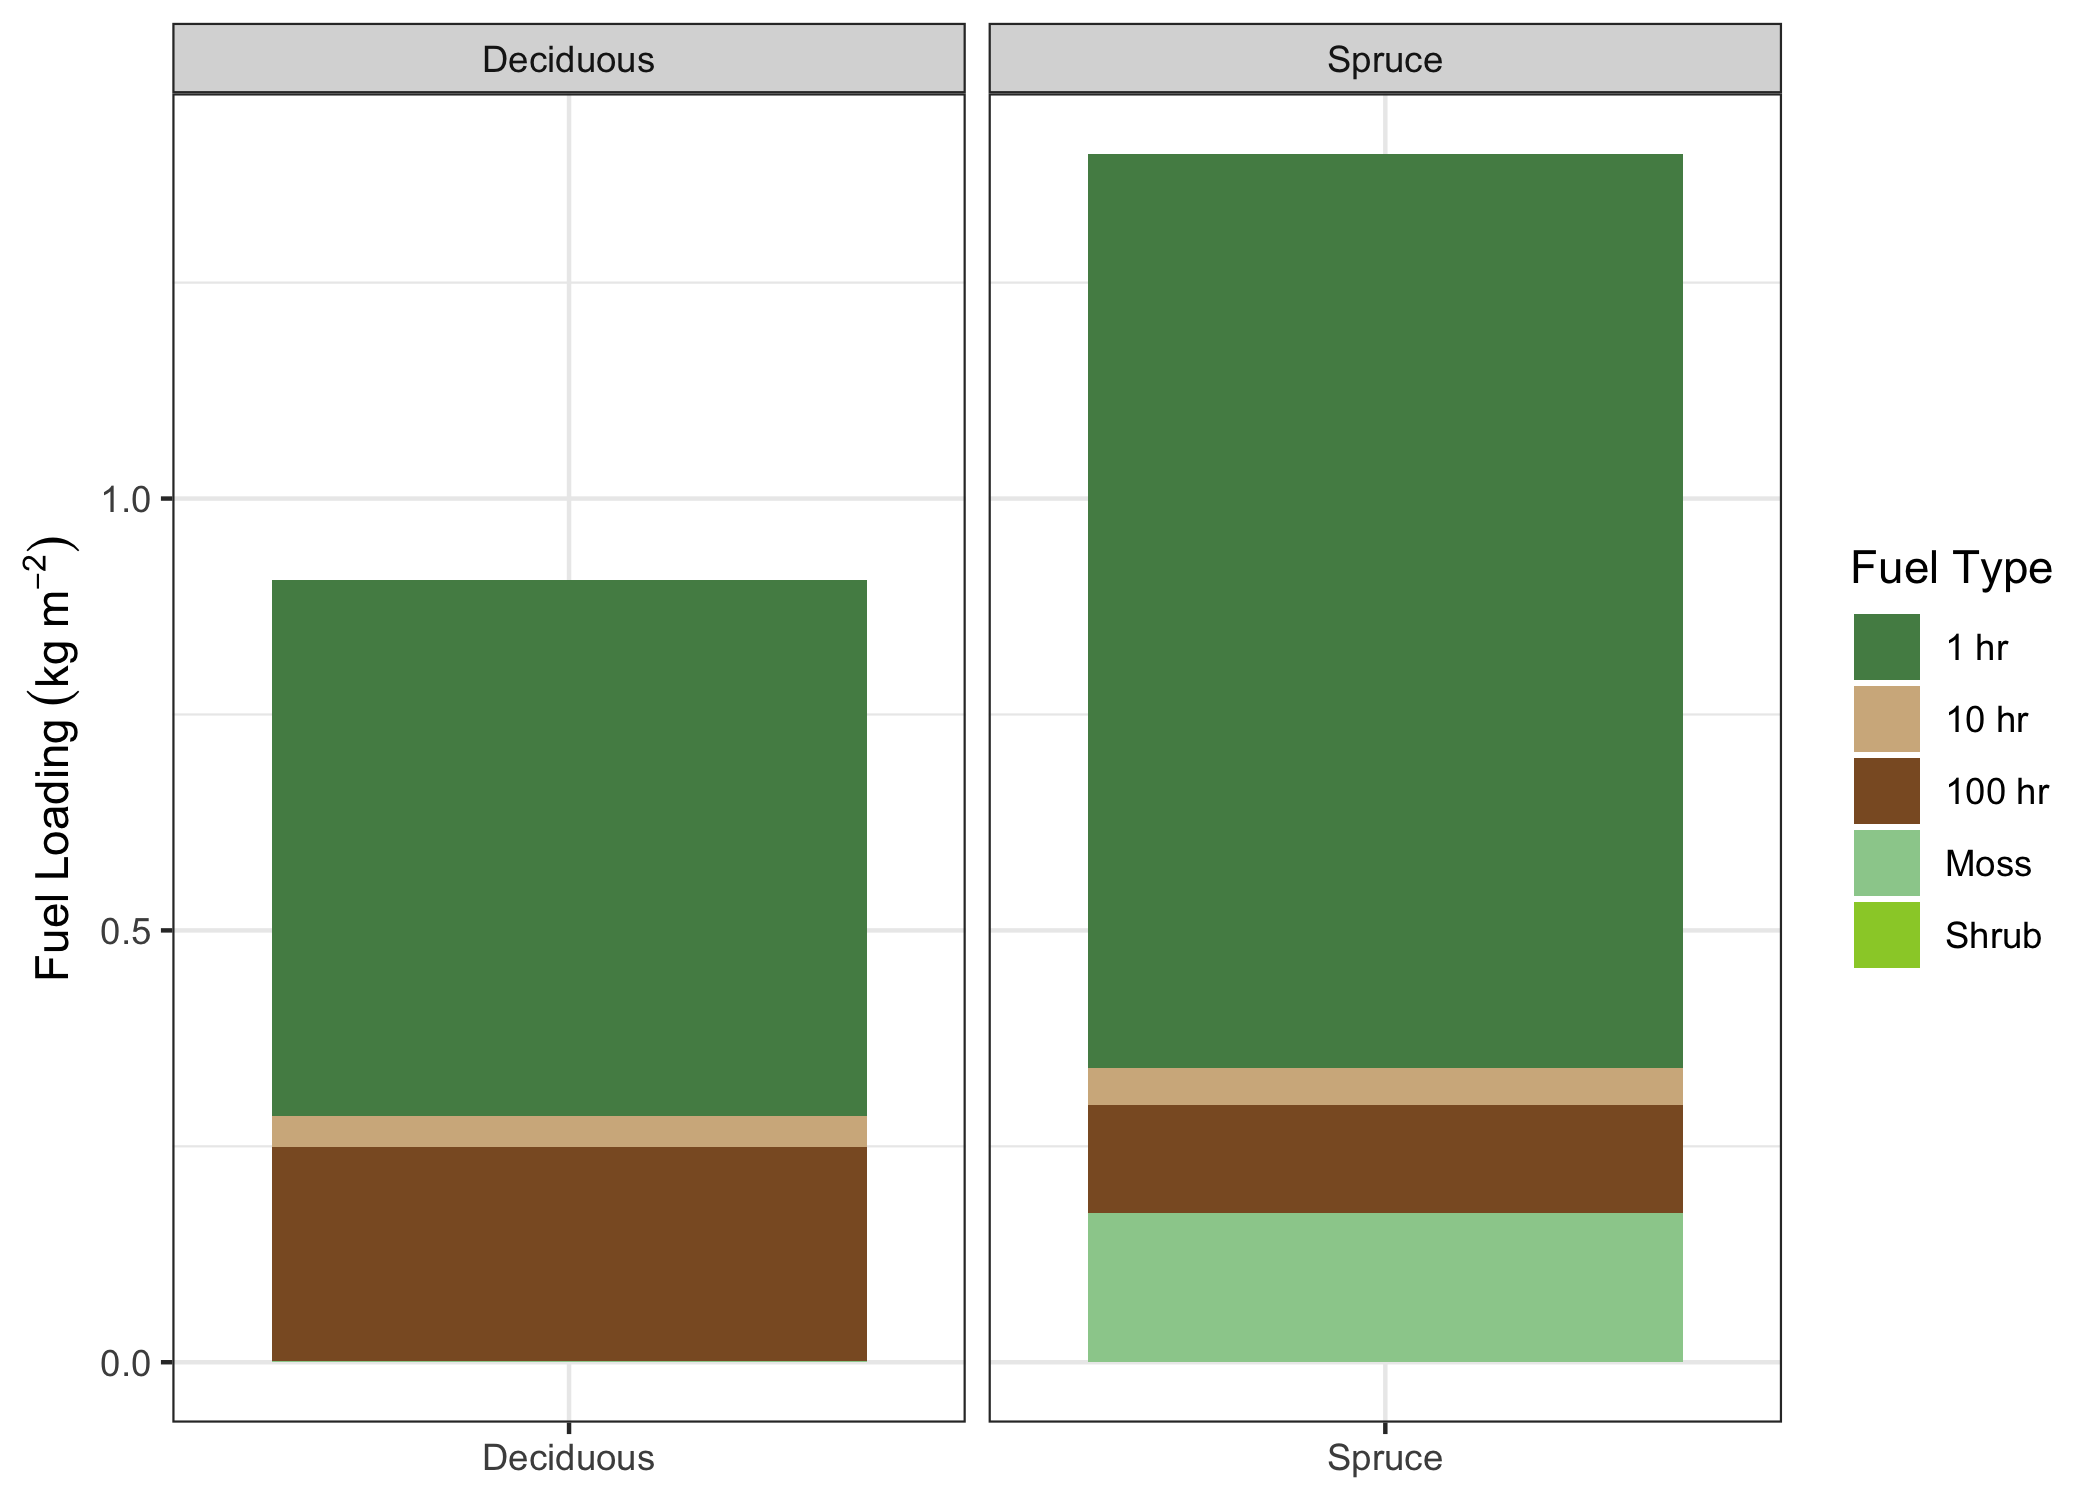
\includegraphics[width=1\linewidth]{Figures/fuel_loading.png}
	\caption{UVAFME-simulated fuel loading by fuel type for a deciduous site and a spruce site.}
	\label{fig:fueltypes}
\end{figure}

As in \citeA{thonickeInfluenceVegetationFire2010}, overall litter bulk density and SAV are calculated as a weighted average of all the litter types' (excluding boles) bulk density and SAV:

\begin{equation} 
	BD = \sum_{i=1}^{8} BD_i\frac{w_i}{w}
\end{equation}

\begin{equation} 
	\sigma = \sum_{i=1}^{8} \sigma_i\frac{w_i}{w}
\end{equation}

where $BD_i$ and $\sigma_i$ are the bulk density and SAV of each litter type and $w_i$ is the fuel loading of each litter type (kg m$^{-2}$), and $w$ is the total fuel loading (kg m$^{-2}$).

Daily fuel moisture of each litter type is calculated based on the Canadian Forest Fire Danger Rating System (CFFRDS) \cite{wangUpdatedSourceCode2015}, which calculates fuel moisture and potential fire conditions based on temperature, precipitation, wind speed, and relative humidity. For this model, we calculate the fine fuel moisture code (FFMC) and duff moisture code (DMC) based on CFFRDS equations. We use the FFMC to calculate fuel moisture for all 1-hr, 10-hr, and 100-hr fuels. We use the DMC to calculate moisture of 1000-hr fuels (i.e. boles) and root litter.  We use equations from the CFFRDS to convert FFMC and DMC to fuel moisture, additionally modified by fuel surface area-to-volume ratio:

\begin{equation} 
	m_{FFMC} = (1/100)\frac{147.2(101.0 - FFMC)}{59.5 + FFMC}\alpha
\end{equation}

\begin{equation} 
	m_{DMC} = (1/100)\Big(20.0 + \frac{100.0}{\text{e}^{(0.023DMC)}}\Big)\alpha
\end{equation}

where $\alpha$ is a litter-type specific parameter for fuel drying, and is calculated based on fuel SAV, modified from an equation in \citeA{thonickeInfluenceVegetationFire2010}.

\begin{equation} 
	\alpha = \text{e}^{(-\sigma/250.0)}
\end{equation}

Moss moisture is calculated as:

\begin{equation} 
	m_{moss} = (1/100)\Big(\frac{199.2(101.0 - FFMC)}{59.5 + FFMC} + 12.0\Big)
\end{equation}

Live shrubs and tree fuel moisture is calculated using the DMC as:

\begin{equation} 
	m_{live} = (1/100)\Big(90.0 + \frac{30.0}{\text{e}^{0.232DMC}}\Big)
\end{equation}

Most fuels can range from over 200\% moisture at very low FFMC or DMC values to close to 0\% moisture at very high FFMC/DMC values (Fig. \ref{fig:fuelmoist}).

\begin{figure}
	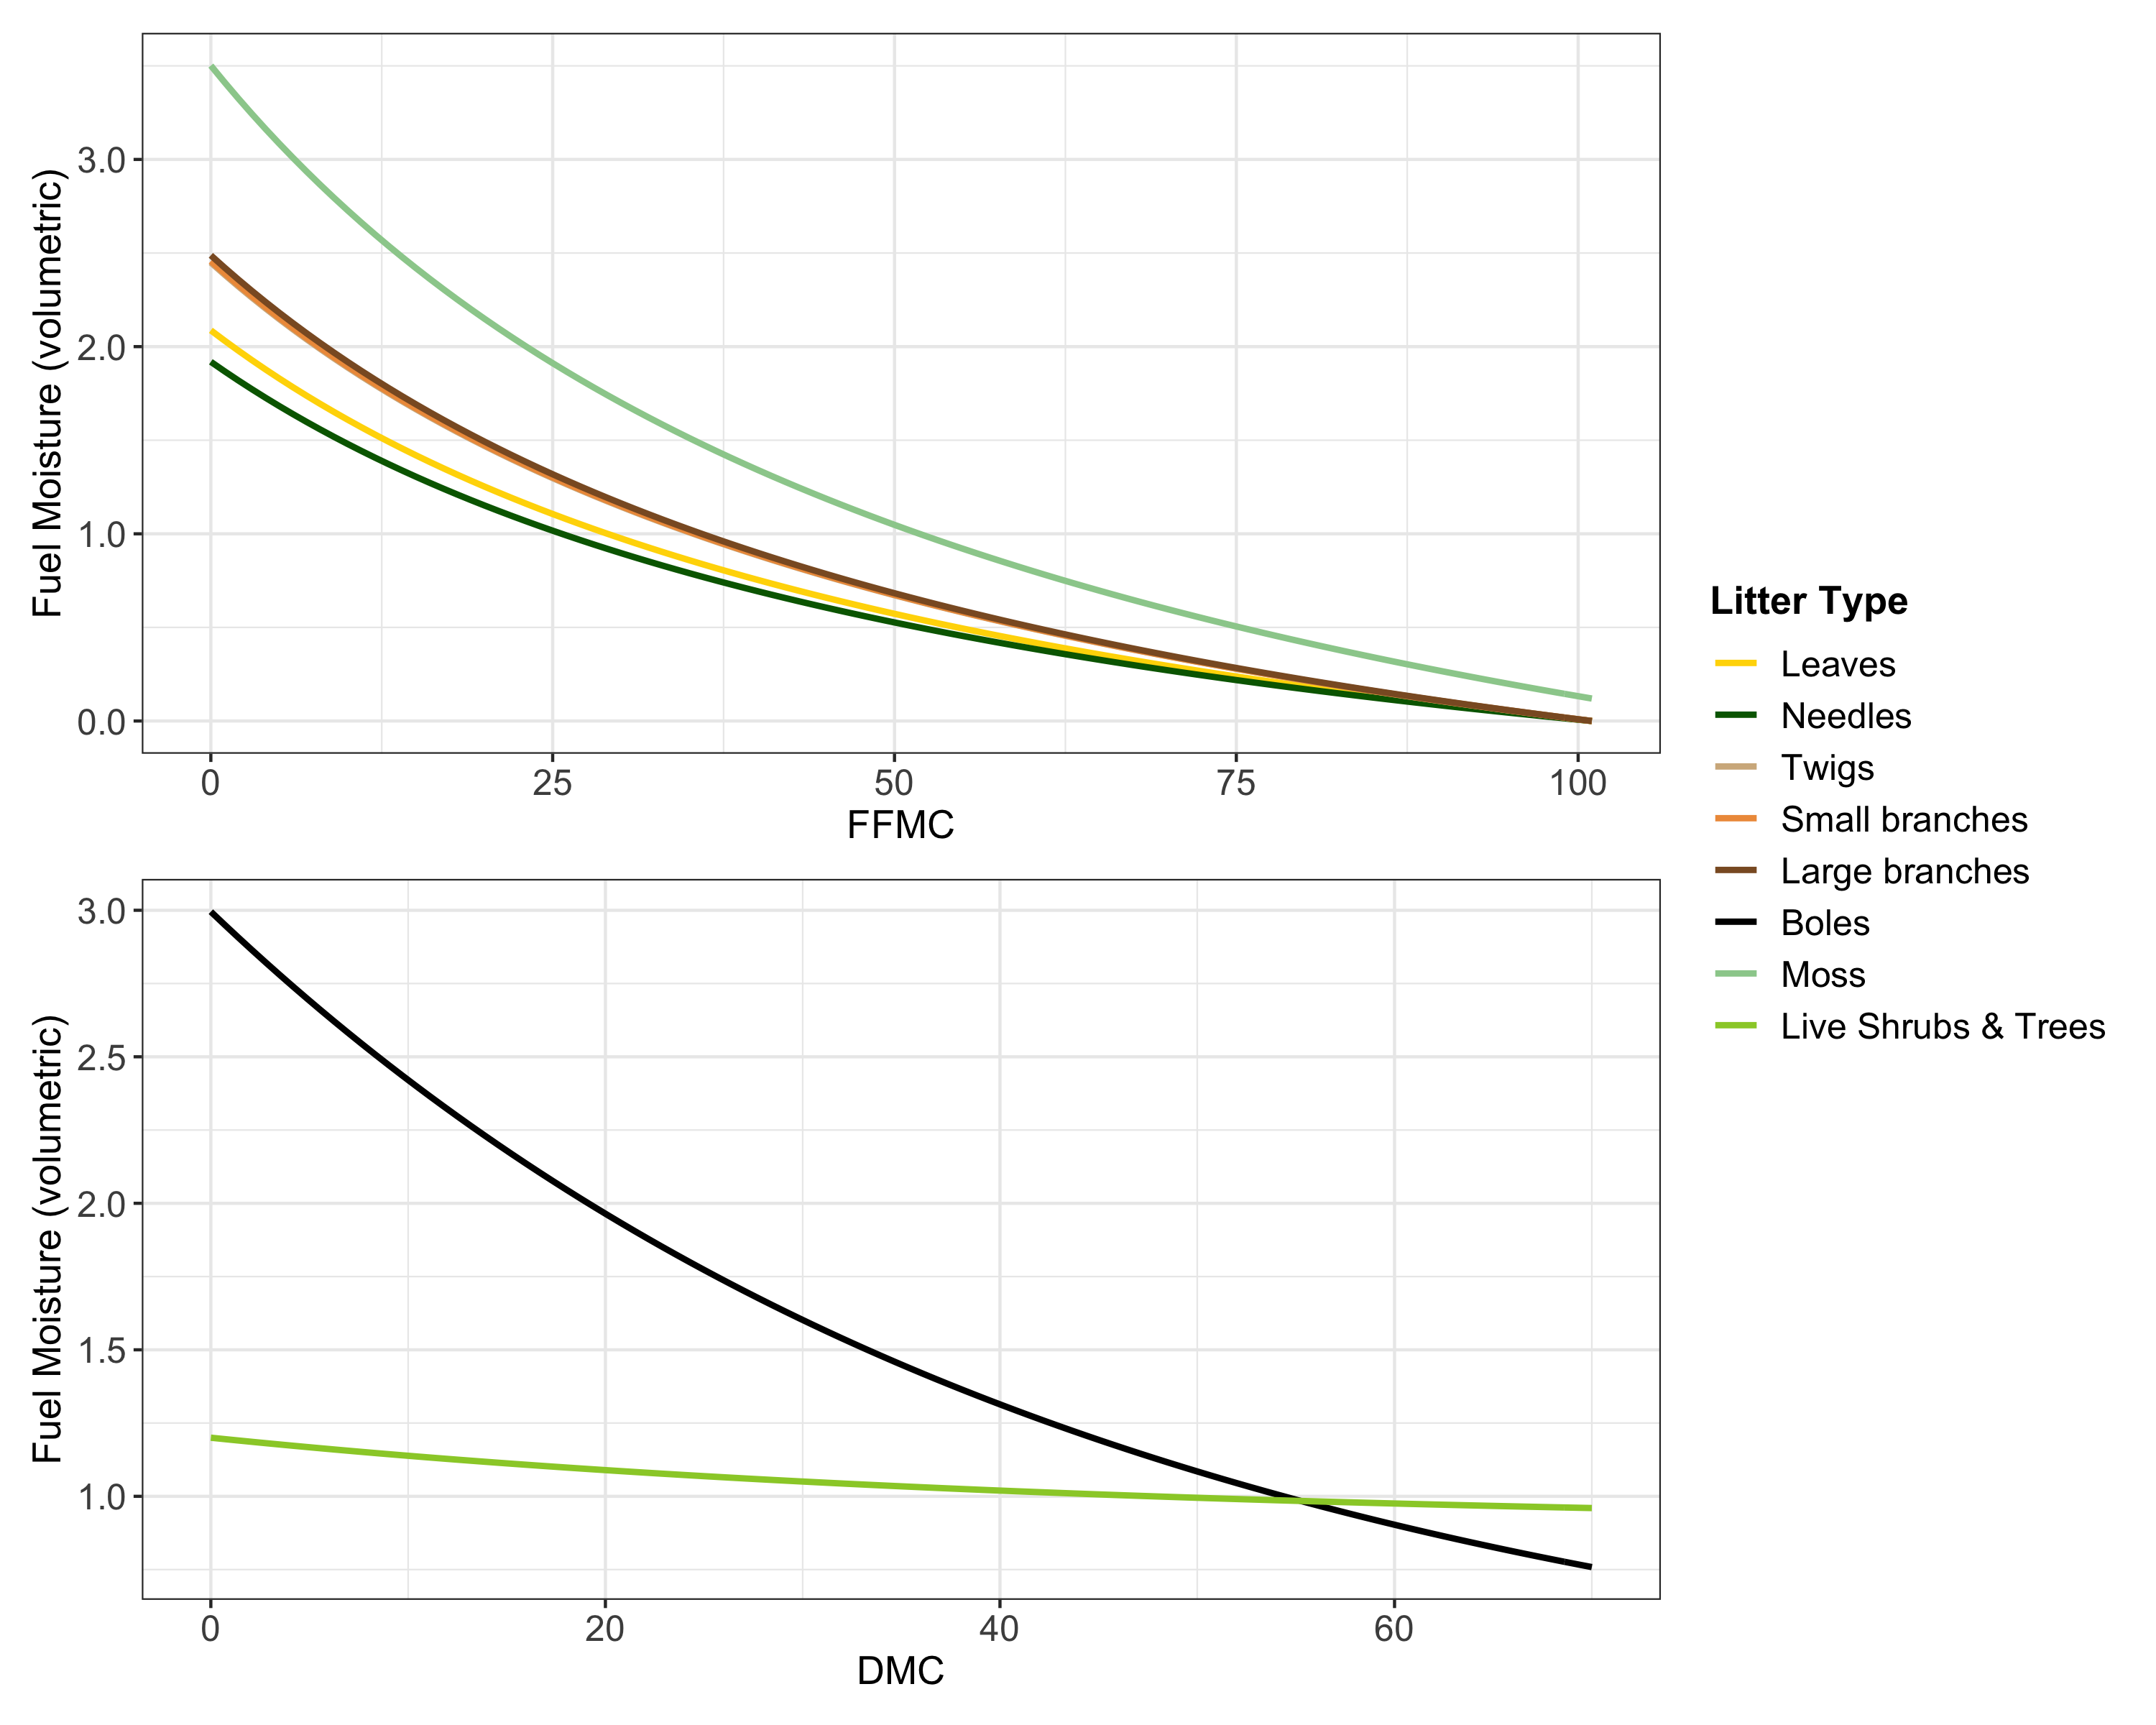
\includegraphics[width=\linewidth]{figures/FuelMoisture.png}
	\caption{Fuel moisture for different fuel types at different FFMC and DMC values.}
	\label{fig:fuelmoist}
\end{figure}

Moisture of extinction, the moisture content (m$^3$ m$^{-3}$) at which the fuel can no longer burn, is calculated as in \cite{petersonModelingPostfireConifer1986}:

\begin{equation}
	m_x = 0.524 - 0.066\text{ln}(\sigma) 
\end{equation}

Moss moisture of extinction is set to 0.76 by default \cite{frandsenIgnitionProbabilityOrganic1997}, and live fuel moisture of extinction is set to 1.0.

Similar to average litter bulk density and SAV, weighted averages are taken of fuel moisture and moisture of extinction:

\begin{equation} 
	m = \sum_{i=1}^{8} m_i\frac{w_i}{w}
\end{equation}

\begin{equation} 
	m_x = \sum_{i=1}^{8} m_{x_i}\frac{w_i}{w}
\end{equation}

\subsubsection{Fire Danger and Ignition Events}

In this updated version, ignition events are considered probabilistic and based on mean average lightning strike frequency ($r_{light}$, strikes day$^{-1}$) and a fire danger index (FDI, 0-1).

\begin{equation} 
	p_{ign} = r_{light}FDI
\end{equation}

\begin{equation} 
	FDI = \text{max}\Big(0.0, 1 - \frac{m}{m_x}\Big)
\end{equation}

calculated as in \citeA{thonickeInfluenceVegetationFire2010} and \citeA{venevskySimulatingFireRegimes2002}. Thus, when lightning strike rates are zero (e.g. in the winter) or when FDI is zero (e.g. for zero fuel or very wet fuel conditions), an ignition event cannot occur. At FDI values of 0.3 or less, fire probability is considered low, FDI values between 0.3 and 0.75 are considered moderate, FDI values between 0.75 and 1.0 are considered high, and at FDI = 1.0, fire conditions are extreme (Fig. \ref{fig:FDIfig}).

\begin{figure}
	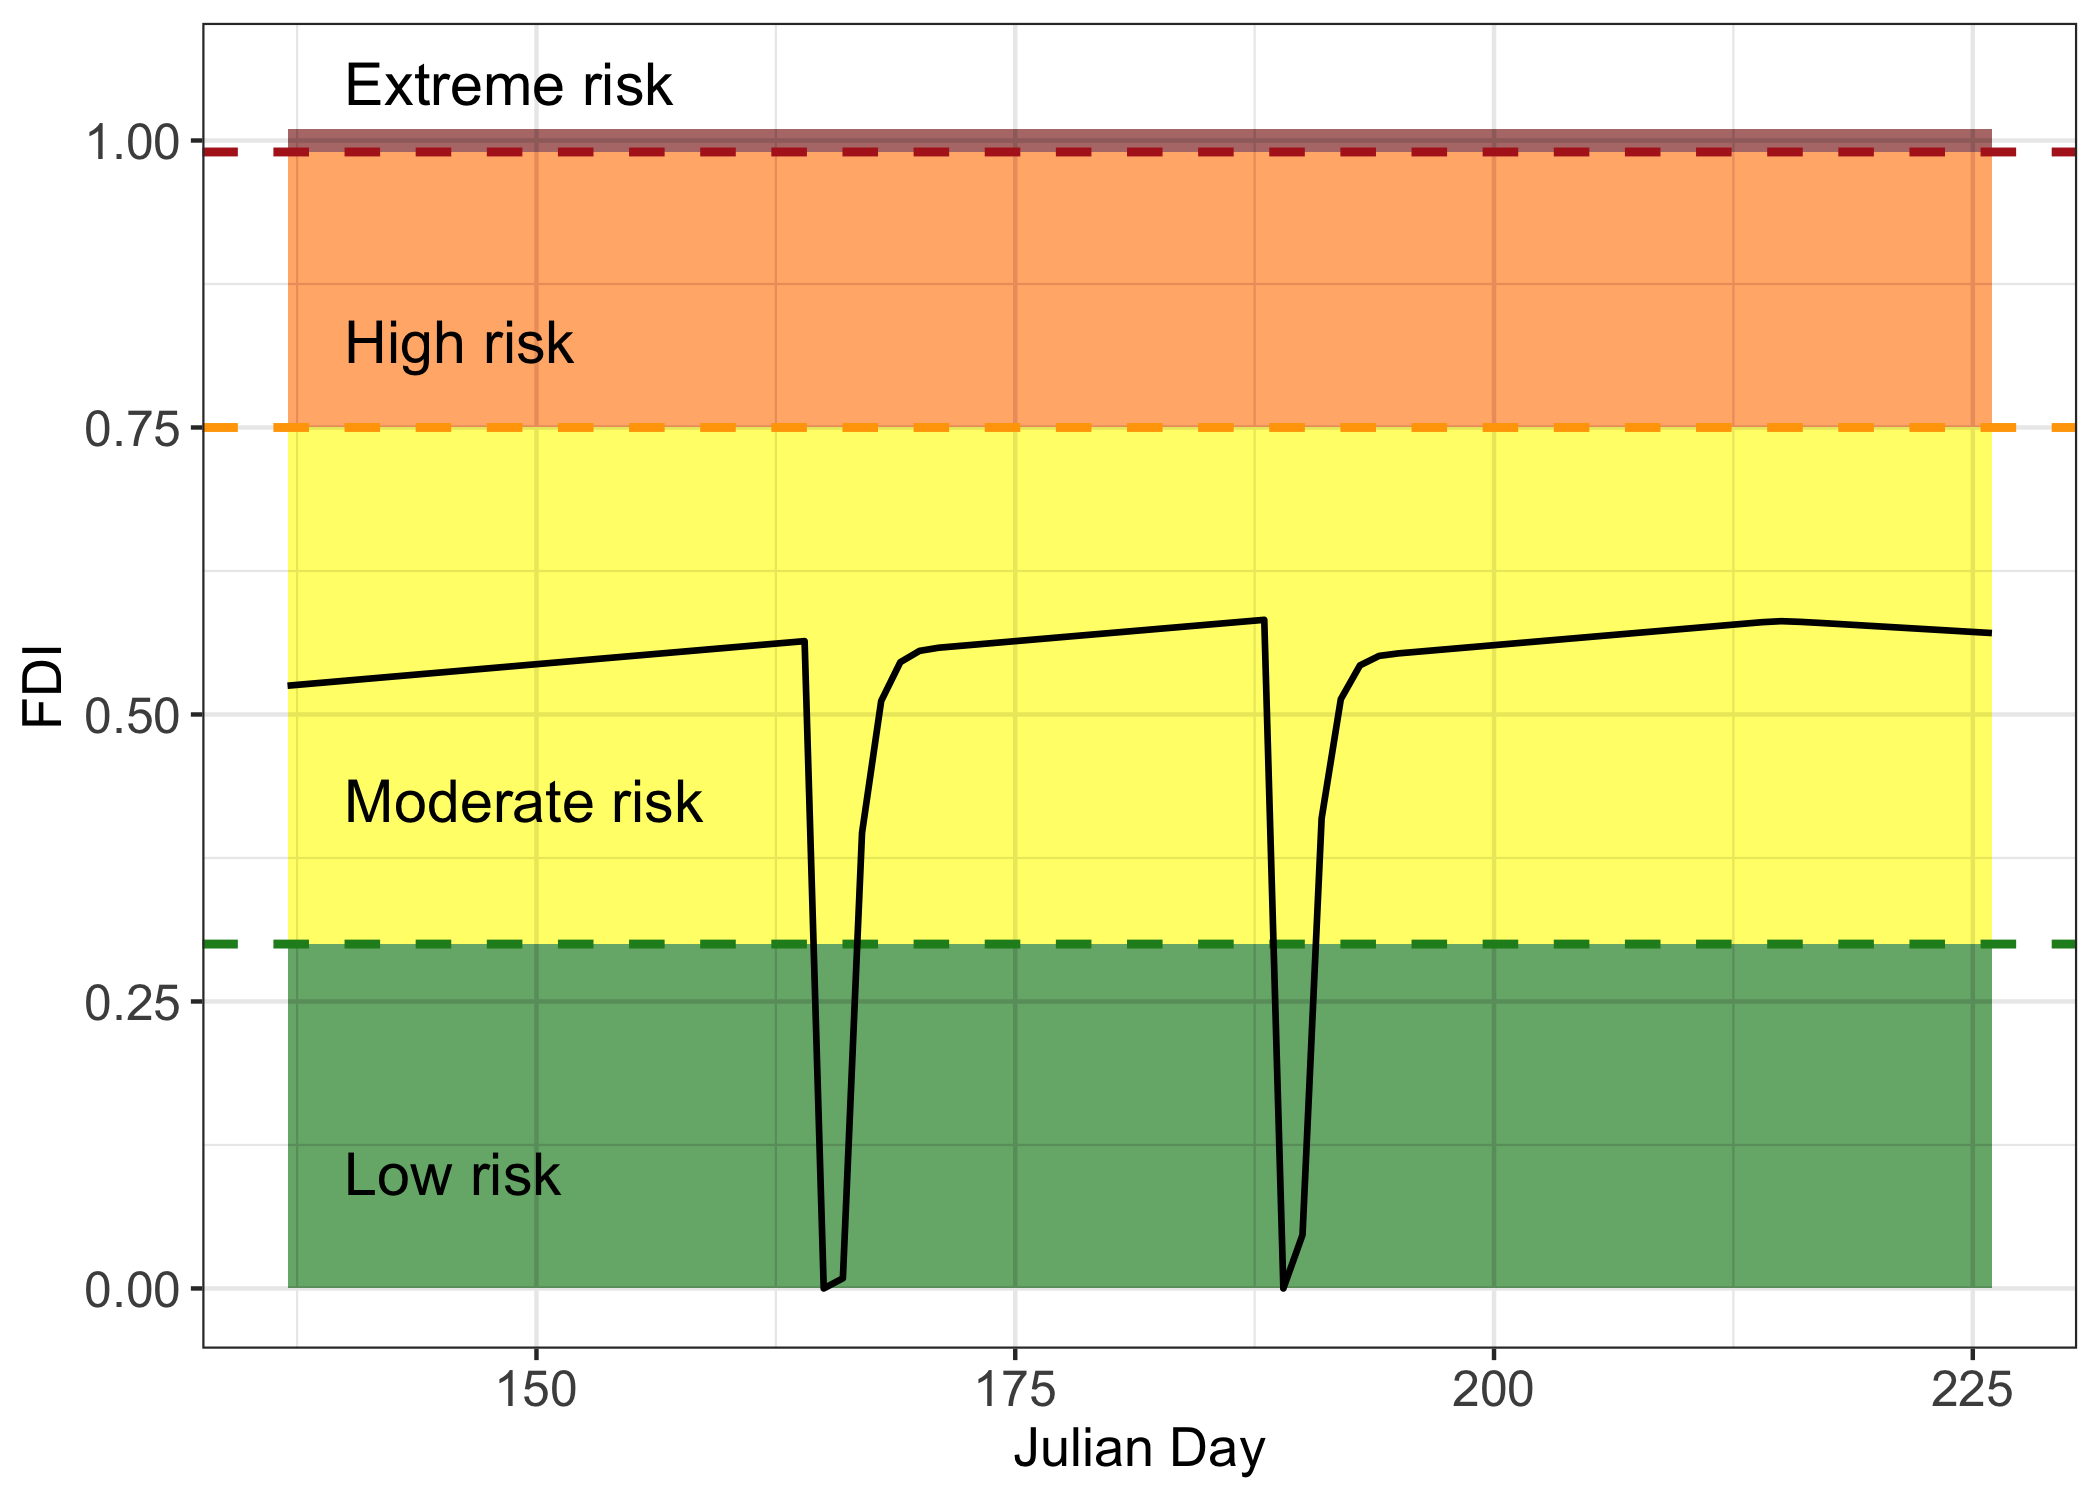
\includegraphics[width=\linewidth]{figures/FDI.png}
	\caption{Simulation of fire danger index (FDI) for one year at a black spruce site in interior Alaska.}
	\label{fig:FDIfig}
\end{figure}

\subsubsection{Rate of Spread}

Once an ignition event does occur, the potential rate of spread ($ROS$, m min$^{-1}$) is calculated based on equations from \citeA{rothermelMathematicalModelPredicting1972}. Fire spread rate can be modeled as the ratio between the heat flux from the flaming front (i.e. the energy available to heat unburned fuel) to the heat required for fuel ignition \cite{johnsonFireVegetationDynamics1992}.

\begin{equation*} 
	\text{ROS} = \frac{\text{energy available to heat unburned fuel}}{\text{heat required for fuel ignition}}
\end{equation*}

The available energy is based on the heat given off by fuel when it is combusted (J kg$^{-1}$) as well as the rate at which the fuel is being burned (kg area$^{-1}$ time $^{-1}$). The heat required is based on fuel physical and chemical properties such as bulk density, SAV, mass, and moisture. As in \citeA{rothermelMathematicalModelPredicting1972}, forward rate of spread ($ROS_f$, m min$^{-1}$) is calculated as:

\begin{equation} \label{eq:ros}
	ROS_f = \frac{I_R \cdot \xi \cdot (1 + \theta_w)}{BD \cdot \epsilon \cdot Q_{ign}}
\end{equation}

where $I_R$ is the reaction intensity (kJ m$^2$ min$^{-1}$) and represents the energy release rate per unit area of the fire front; $\xi$ is the propagating flux ratio, and represents the proportion of $I_R$ that heats adjacent fuel particles to ignition; $\theta_w$ is a wind factor; $\epsilon$ is the effective heating number and represents the proportion of fuel particles that are heated to ignition temperature; and $Q_{ign}$ is the heat of pre-ignition (kJ kg$^{-1}$), which is the amount of heat required to ignite a given mass of fuel. All the variables within this equation depend on the fuel characteristics described above as well as wind speed.

Reaction intensity ($I_R$, kJ m$^2$ min$^{-1}$) is calculated as:

\begin{equation} \label{eq:ir}
	I_R = \Gamma ' \cdot w_n \cdot h \cdot \eta_m \cdot \eta_s
\end{equation}

where $\Gamma '$ is the optimum reaction velocity (min$^{-1}$), which indicates completeness and rate of fuel consumption; $w_n$ is the mineral fuel load (kg m$^{-2}$), calculated as $w_n = w(1 - S_T)$, where $S_T$ is the fractional mineral content, set to 0.055 \cite{thonickeInfluenceVegetationFire2010}.  The heat content of the fuel ($h$) is set to a default value of 18,000 kJ kg$^{-1}$, and $\eta_m$ and $\eta_s$ are moisture- and mineral-dampening coefficients, respectively.

Optimum reaction velocity is calculated as the ratio of reaction zone efficiency to reaction time, and is based on fuel conditions (i.e. particle size and fuel bed bulk density). As in \citeA{pyneIntroductionWildlandFire1996}, $\Gamma '$ is calculated as:

\begin{equation} \label{eq:gamma}
	\Gamma ' = \Gamma_{max} \Big( \frac{\beta}{\beta_{opt}}\Big)^A\text{exp}\Big[A\Big(1 - \frac{\beta}{\beta_{opt}}\Big)\Big]
\end{equation}

where $\beta$ is the packing ratio, calculated as $\beta = BD/\rho_p$, where $\rho_p$ is the oven-dry particle density, set to 513 kg m$^{-3}$ \cite{pyneIntroductionWildlandFire1996}. $\beta_{opt}$ is the optimum packing ratio and is calculated as $\beta_{opt} = 0.200395\sigma^{-0.8189}$ \cite{thonickeInfluenceVegetationFire2010}; and $A = 8.9033\sigma^{-0.7913}$ \cite{brownPredictingVegetationTypes1994, pyneIntroductionWildlandFire1996}.

Maximum reaction velocity ($\Gamma_{max}$, min$^{-1}$) is calculated as:

\begin{equation} 
	\Gamma_{max} = \frac{1}{0.0591 + 2.926\sigma^{-1.5}}
\end{equation}

Higher optimum reaction velocities result in higher rates of spread (Eq. \ref{eq:ir} \& \ref{eq:gamma}), and thus the fuel geometry (i.e. bulk density and SAV) are highly influential on ROS. Low reaction velocities occur at two extremes of fuel compactness and particle size -- loose and dense. In loose beds, low reaction velocities and thus low ROS occurs due to heat transfer losses between particles. In dense beds, low reaction velocities and thus low ROS occurs due to low air-to-fuel ratios and poor penetration of heat at depth \cite{johnsonFireVegetationDynamics1992}. Thus, there is an optimum combination of compactness and particle size that will maximize reaction velocity (Fig. \ref{fig:velocity}).

\begin{figure}
	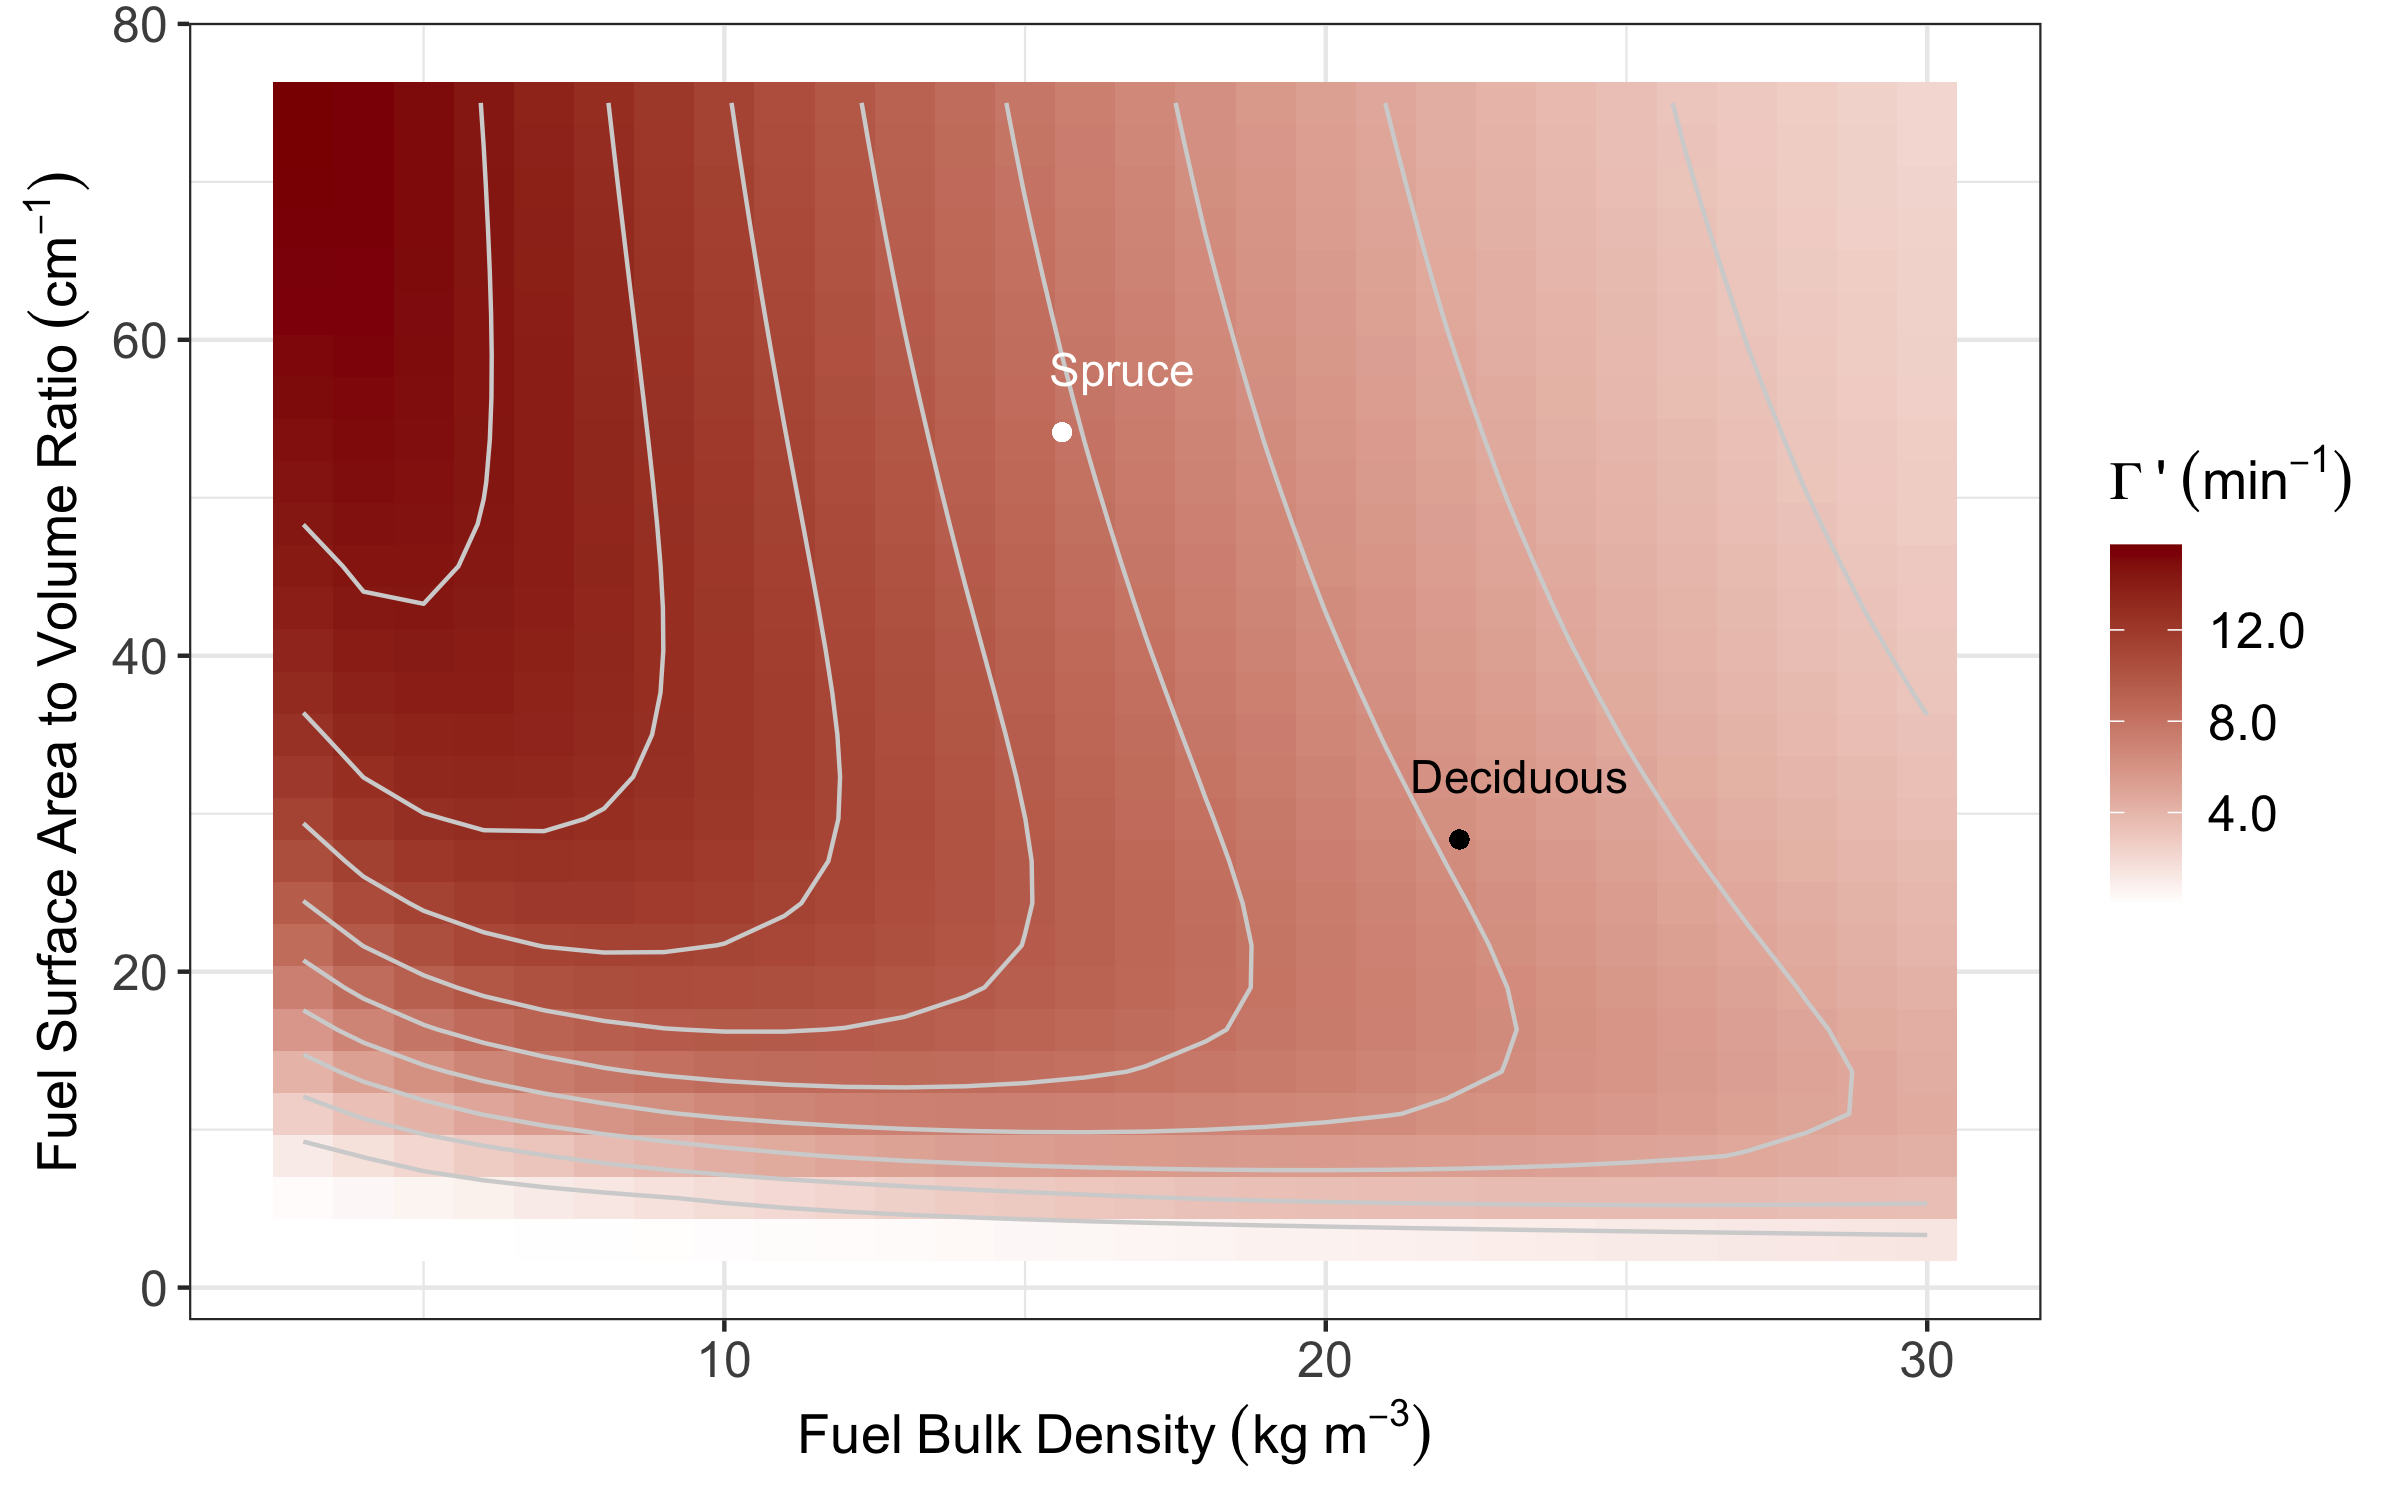
\includegraphics[width=\linewidth]{figures/rvol.png}
	\caption{Effect of fuel SAV and bulk density on optimum reaction velocity ($\Gamma '$, min$^{-1}$). Points show example fuel geometry values for a spruce ($BD \approx$ 16 kg m$^{-3}$, $\sigma \approx$ 54 cm $^{-1}$) and deciduous ($BD \approx$ 22 kg m$^{-3}$, $\sigma \approx$ 28 cm $^{-1}$) site. Spruce litter has lower bulk density and a higher SAV than the litter at the deciduous site, resulting in a higher optimum reaction velocity.}
	\label{fig:velocity}
\end{figure}

The moisture dampening coefficient ($\eta_m$, 0 to 1) is calculated based on the ratio of fuel moisture to moisture of extinction \cite{pyneIntroductionWildlandFire1996} (Fig \ref{fig:moistfig}).

\begin{equation} 
	\eta_m = \text{max}\Bigg(0.0, 1.0 - 2.59\Big(\frac{m}{m_x}\Big) + 5.11\Big(\frac{m}{m_x}\Big)^2 - 3.52\Big(\frac{m}{m_x}\Big)^3\Bigg)
\end{equation}

\begin{figure}
	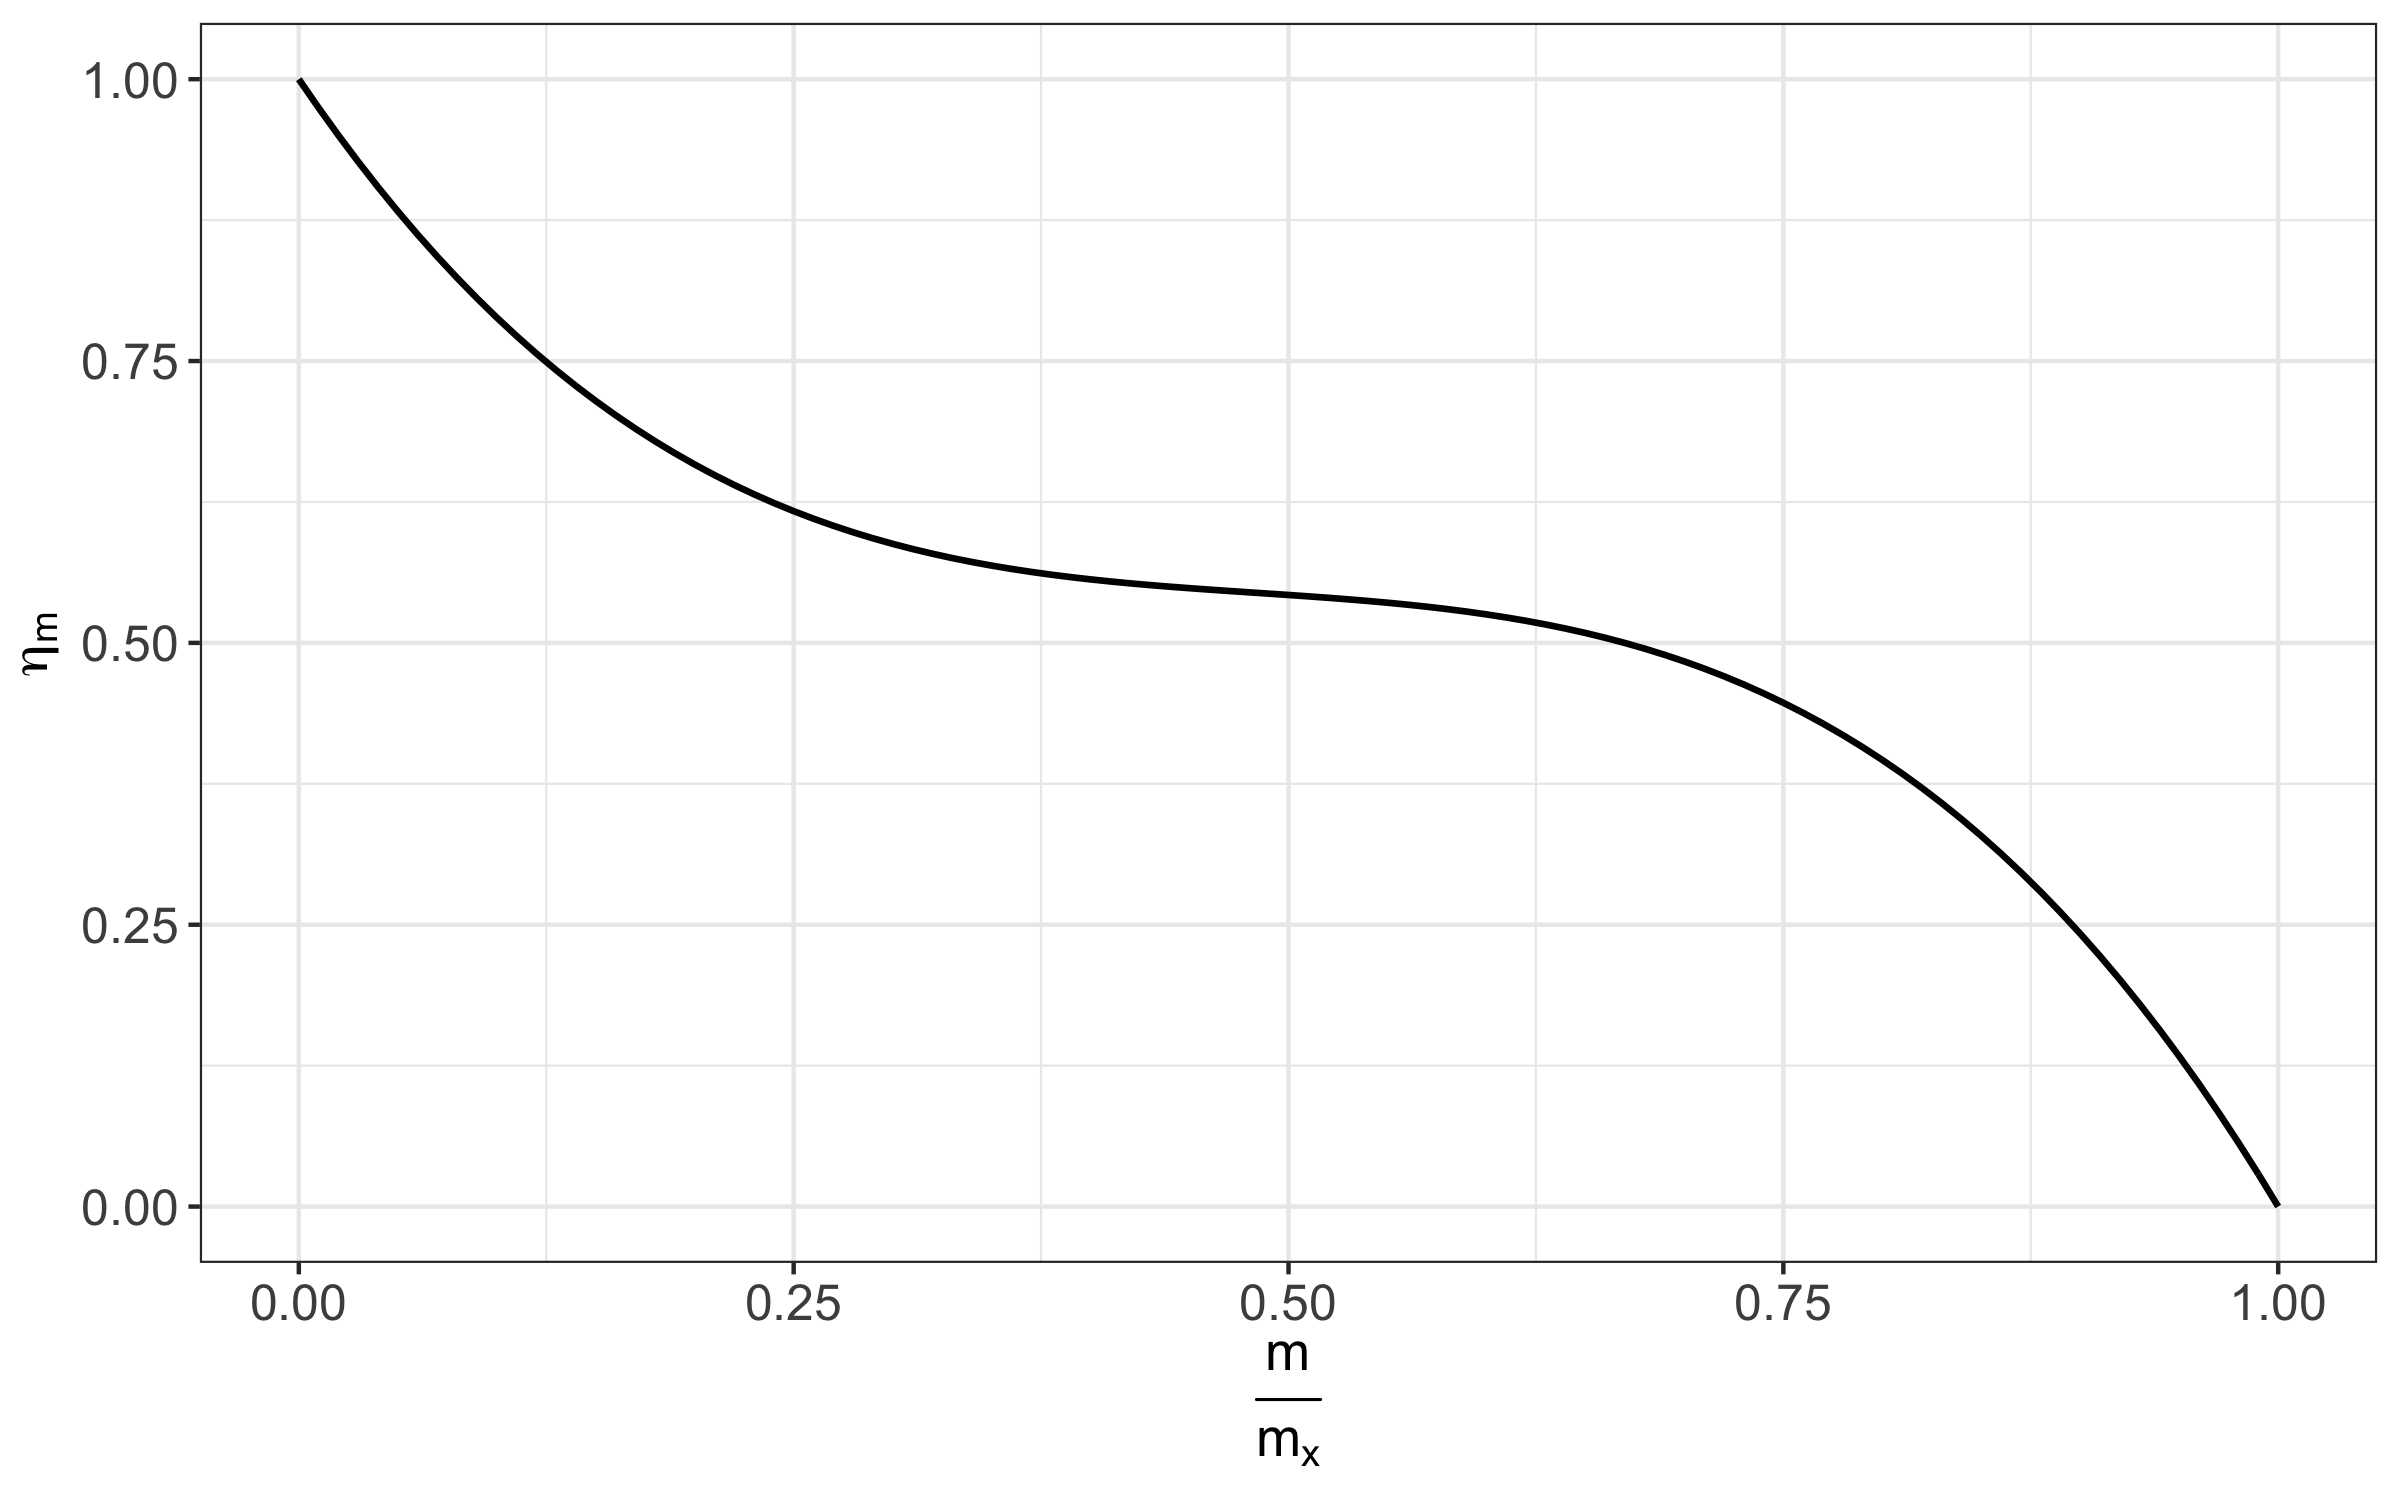
\includegraphics[width=\linewidth]{figures/moist.png}
	\caption{Relationship between the fraction of fuel moisture to moisture of extinction and the moisture dampening coefficient. Moisture values close to or above the moisture of extinction result in very low values of $\eta_m$.}
	\label{fig:moistfig}
\end{figure}

The mineral dampening coefficient ($\eta_S$, 0 to 1) is calculated as $\eta_S = 0.174S_E^{-0.19}$, where $S_E$ is the effective mineral content, set to a default of 0.01 such that $\eta_S$ is a default of 0.41739 \cite{pyneIntroductionWildlandFire1996}.

The propagating flux ratio ($\xi$), relates the propagating flux to the reaction intensity, and is based on fuel bulk density and SAV \cite{rothermelMathematicalModelPredicting1972}.

\begin{equation}
	\xi = \frac{\text{exp}\Big[(0.792 + 3.7597\sqrt{\sigma)}(\beta + 0.1)\Big]}{192.0 + 7.9095\sigma}
\end{equation}

Increasing values of $\xi$ lead to higher rates of spread and higher $\xi$ occurs with higher fuel bulk density and higher fuel SAV (Fig. \ref{fig:fluxrat}).

\begin{figure}
	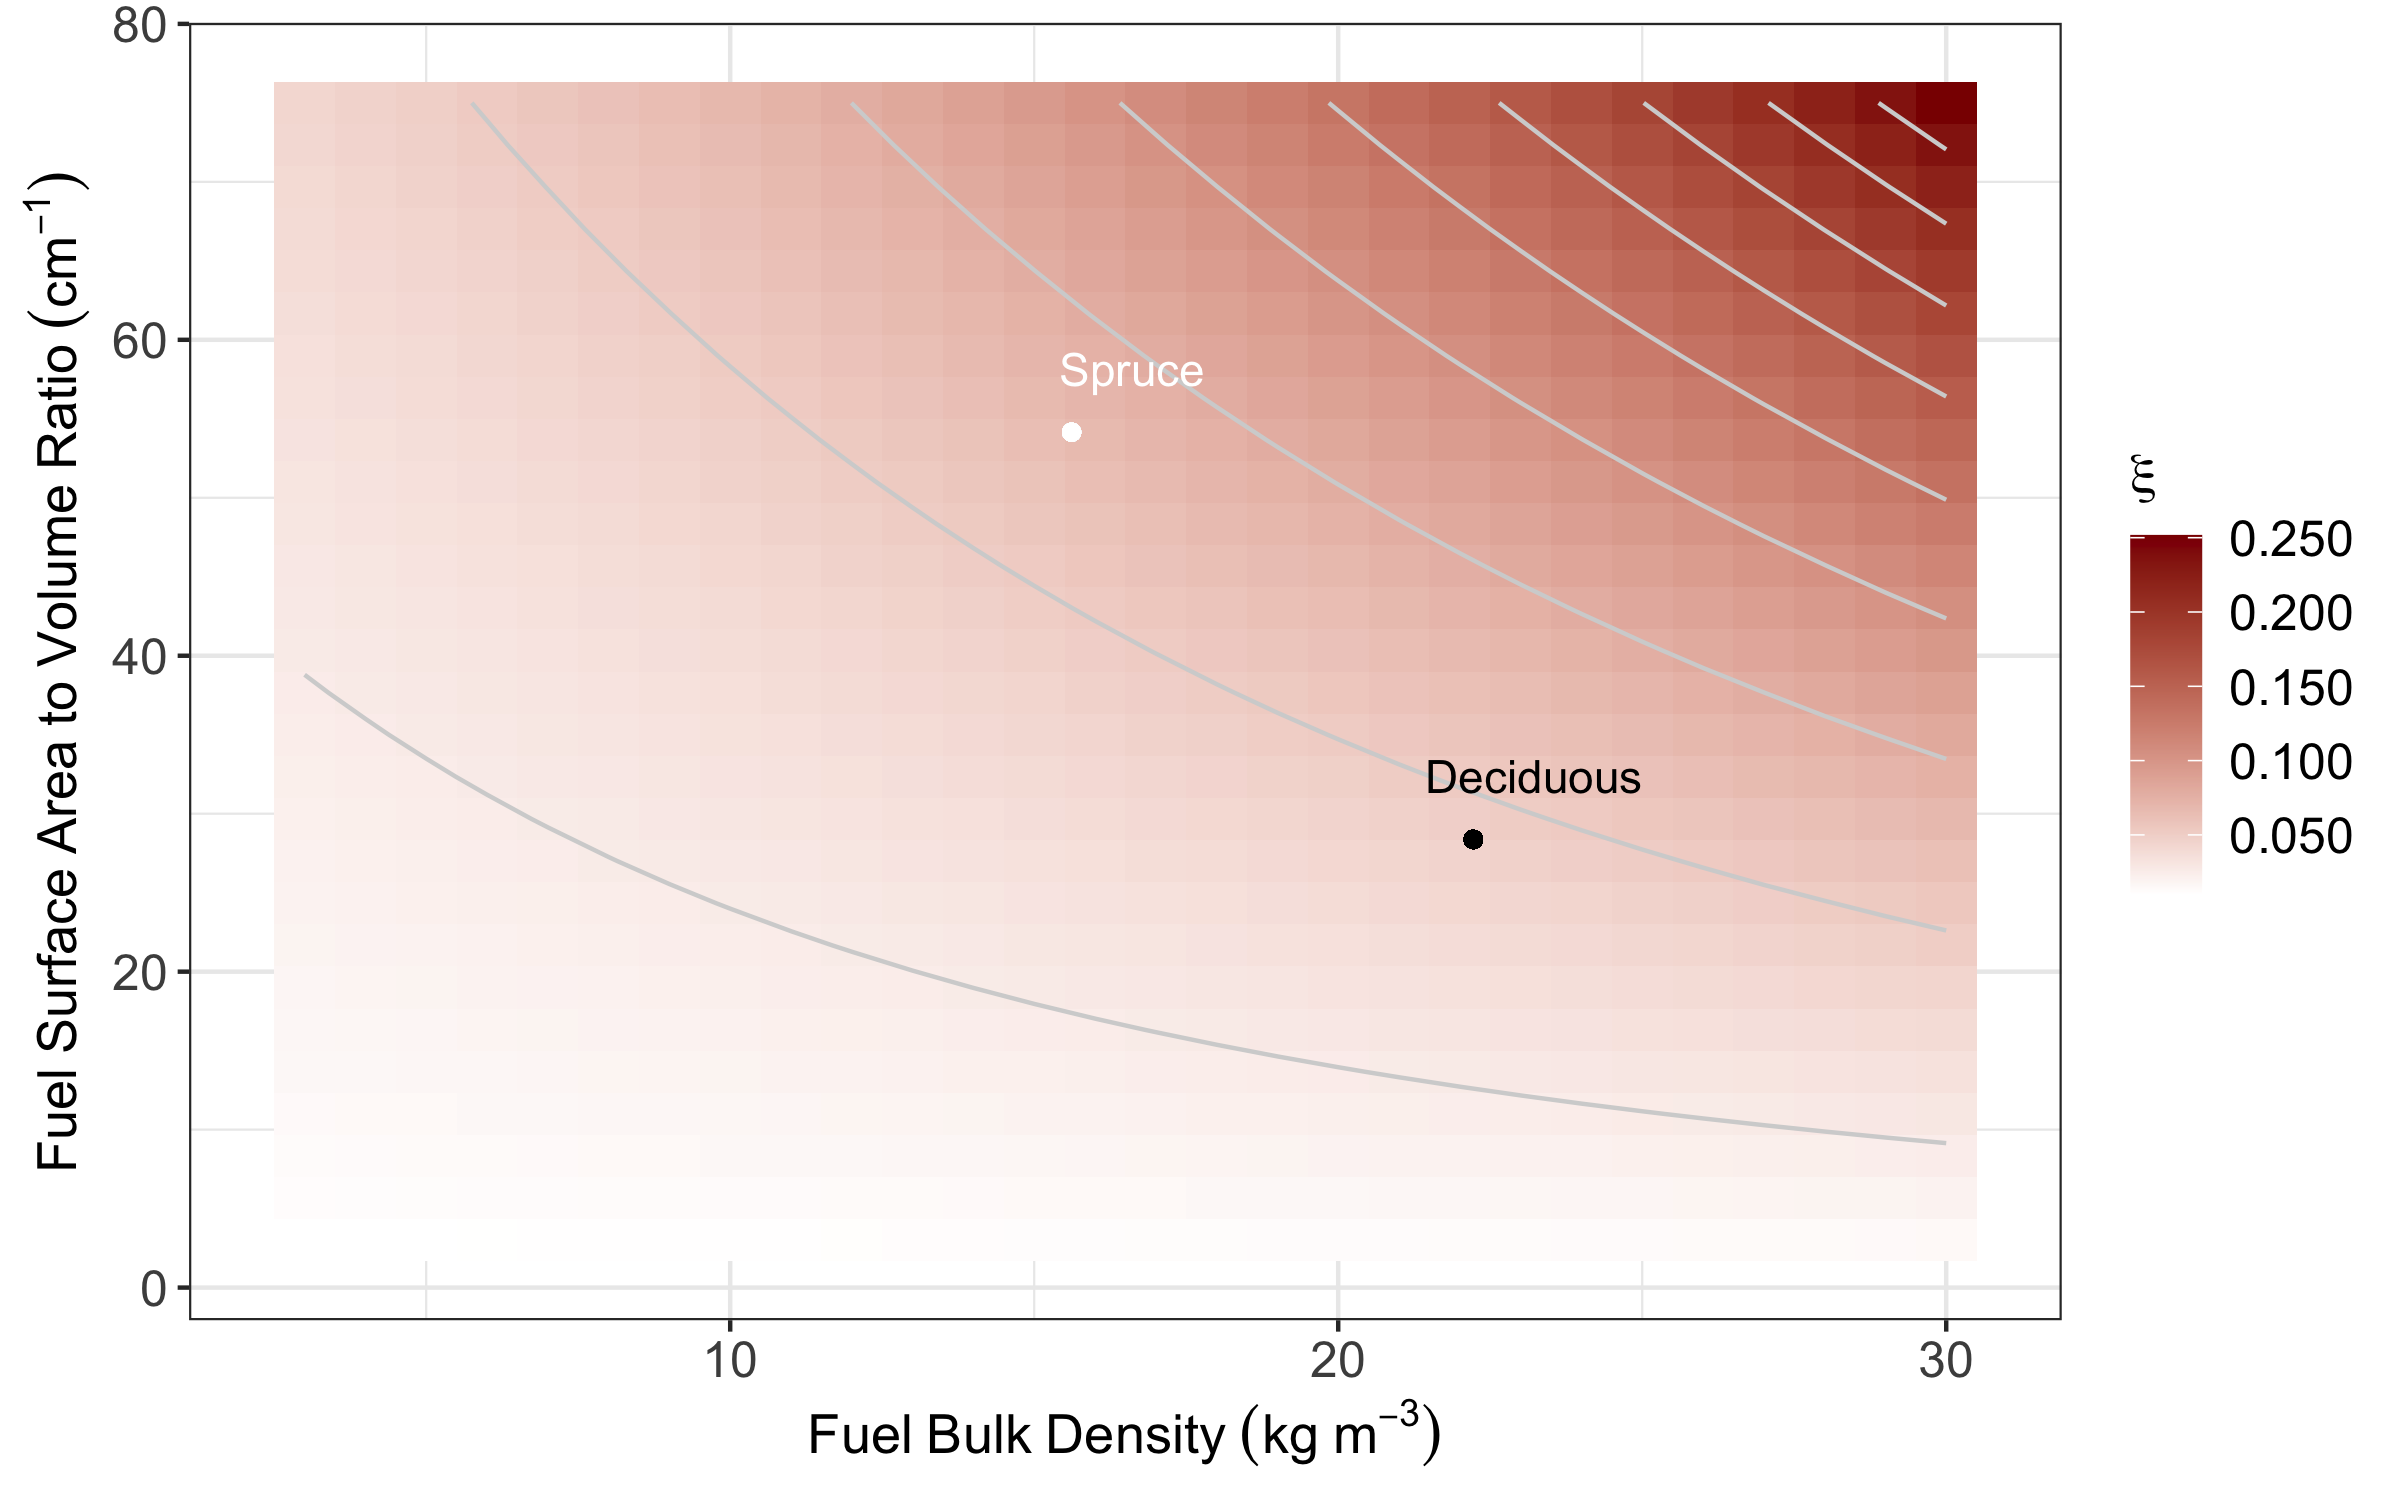
\includegraphics[width=\linewidth]{figures/fluxrat.png}
	\caption{Effect of fuel SAV and bulk density on propagating flux ratio ($\xi$). Points show example fuel geometry values for a spruce ($BD \approx$ 16 kg m$^{-3}$, $\sigma \approx$ 54 cm $^{-1}$) and deciduous ($BD \approx$ 22 kg m$^{-3}$, $\sigma \approx$ 28 cm $^{-1}$) site.}
	\label{fig:fluxrat}
\end{figure}

The combined effects of propagating flux ratio and reaction intensity show the relationship between available energy and fuel geometry, given equal fuel loading and moisture (Fig. \ref{fig:reaction}).

\begin{figure}
	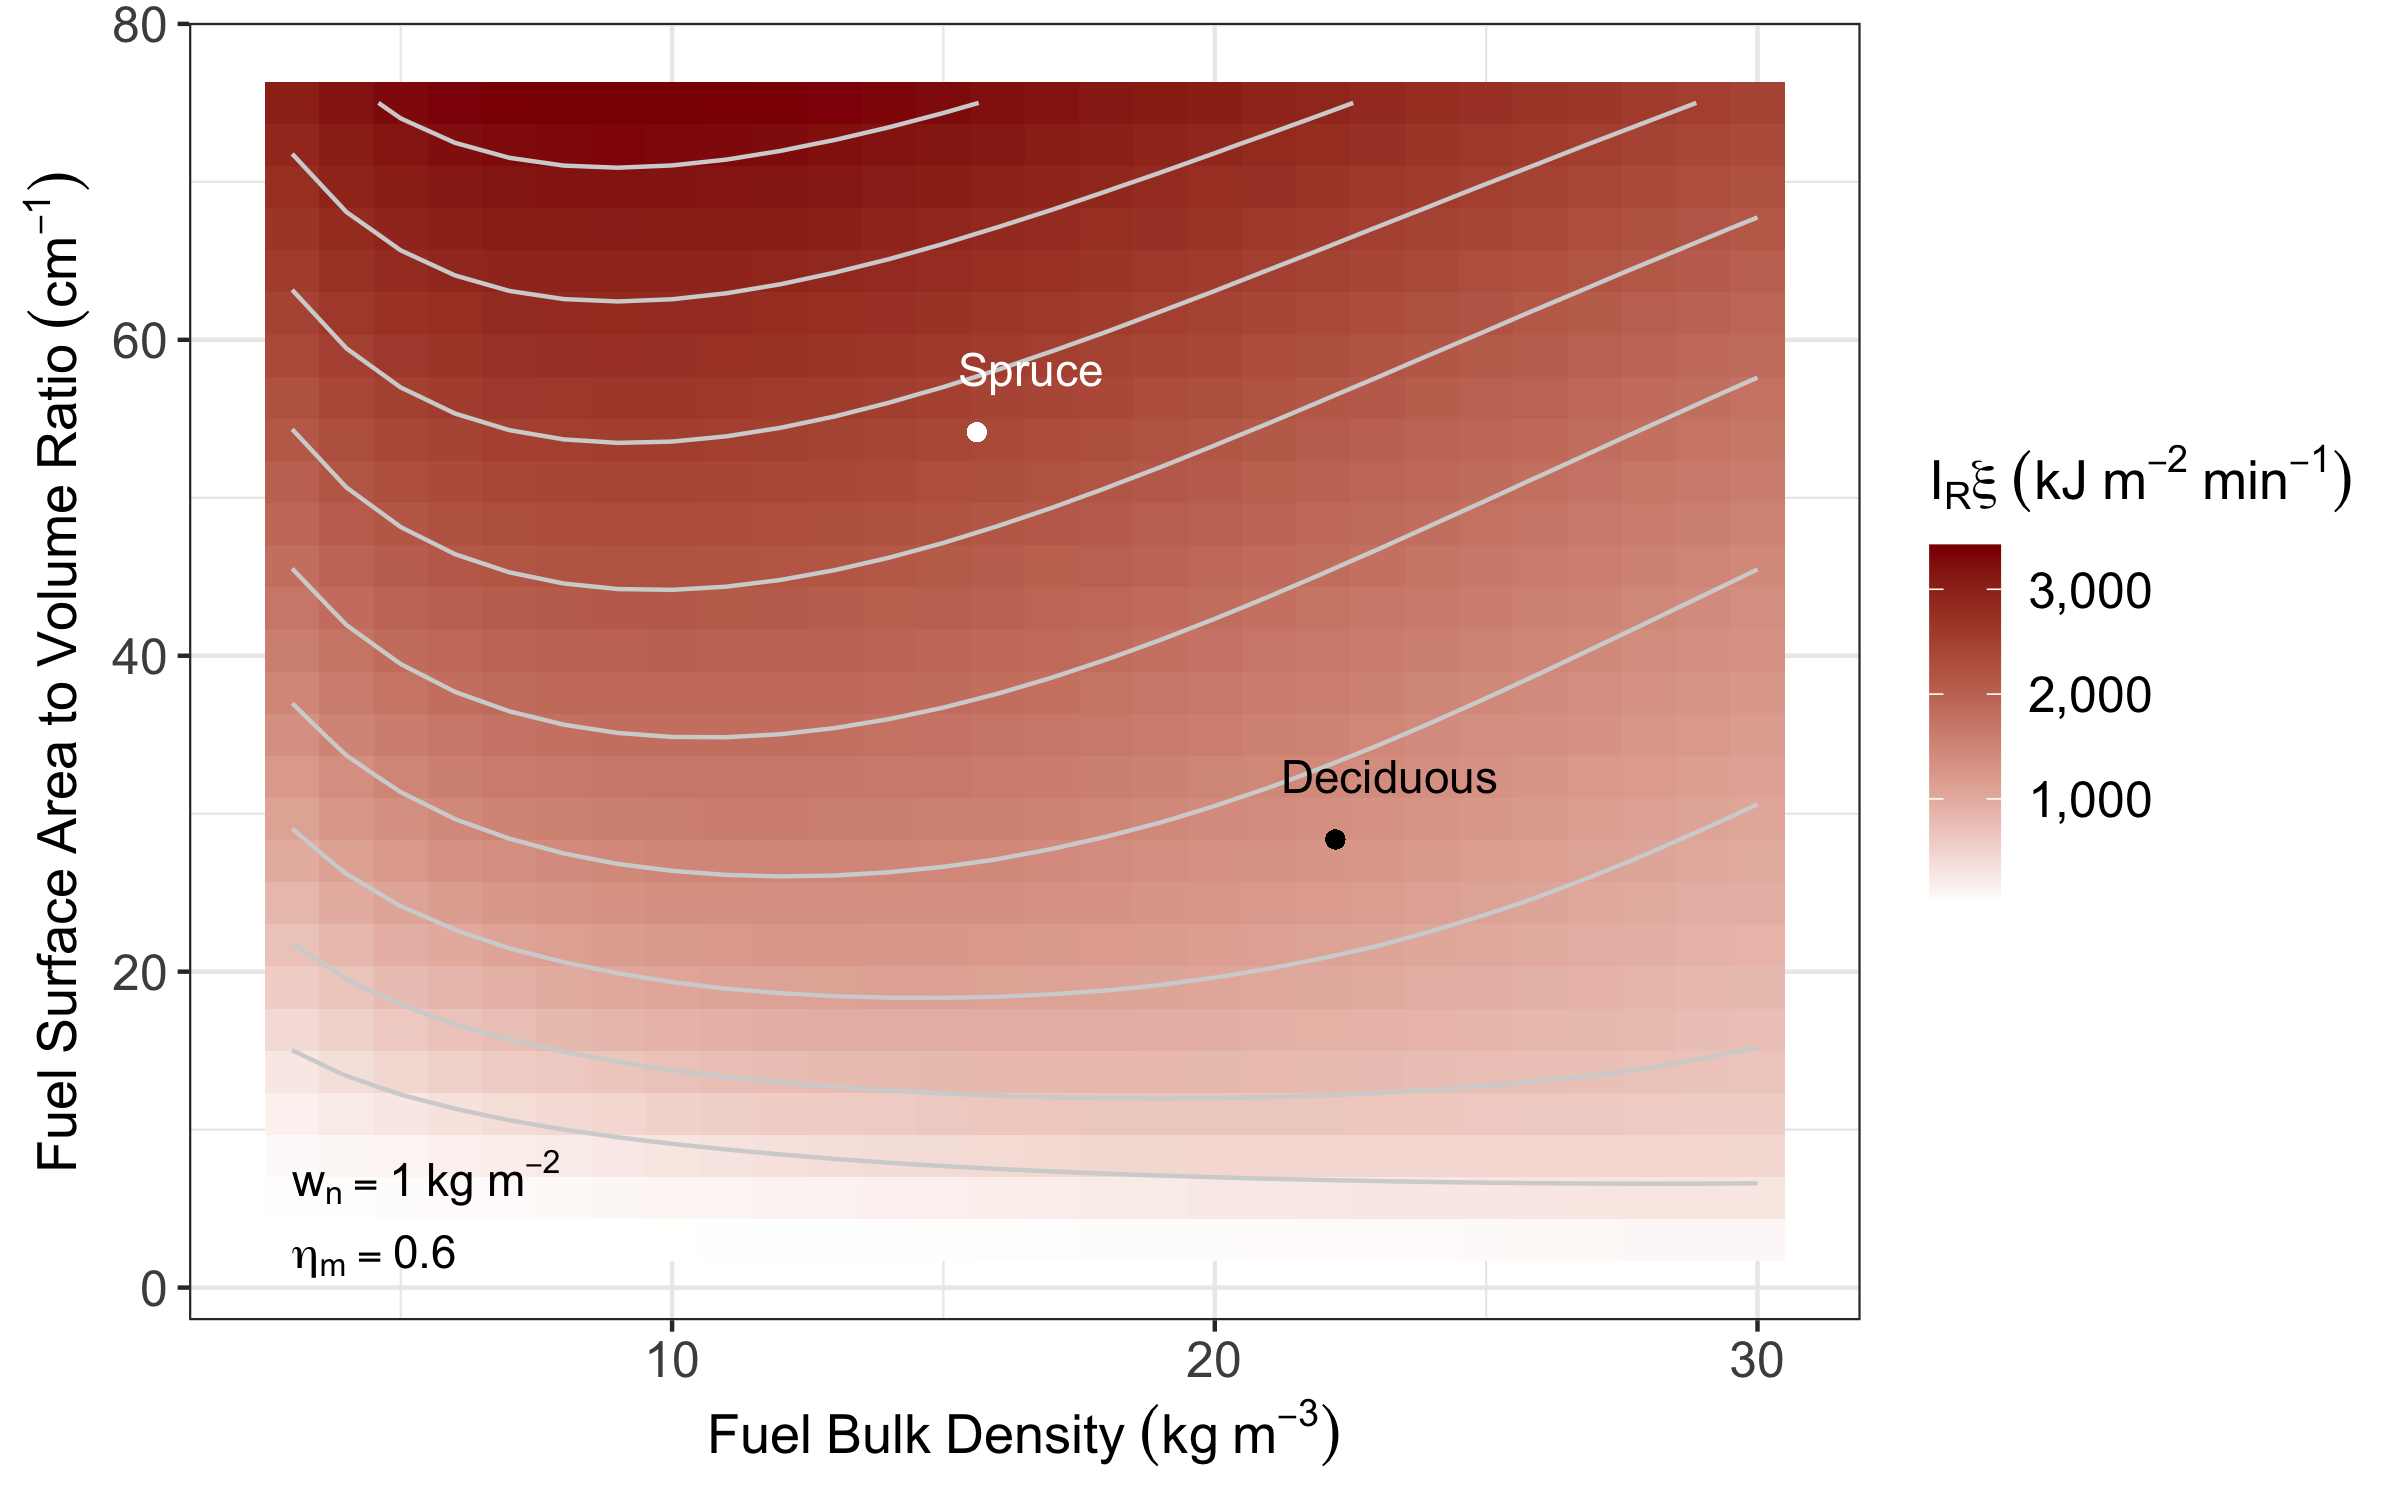
\includegraphics[width=\linewidth]{figures/reaction_intensity.png}
	\caption{Effect of fuel SAV and bulk density on reaction intensity and propagating flux ratio, given equal fuel loading and fuel moisture. Points show example fuel geometry values for a spruce ($BD \approx$ 16 kg m$^{-3}$, $\sigma \approx$ 54 cm $^{-1}$) and deciduous ($BD \approx$ 22 kg m$^{-3}$, $\sigma \approx$ 28 cm $^{-1}$) site.}
	\label{fig:reaction}
\end{figure}

The wind factor ($\theta_w$) is calculated based on wind speed ($U$, m min$^{-1}$) and fuel geometry \cite{thonickeInfluenceVegetationFire2010, rothermelMathematicalModelPredicting1972}. As in \citeA{andrewsExaminationWindSpeed2013} we cap wind speed at a maximum of $U_{max} = 13.12926{I_R}^{\frac{1}{3}}$.

\begin{equation}
	\theta_w = C3.281U^B\Big(\frac{\beta}{\beta_{opt}}\Big)^{-E}
\end{equation}

where $C = 7.747\text{e}^{(-0.8711\sigma^{-0.55})}$, $B = 0.15988\sigma^{0.54}$, and $E = 0.7515\text{e}^{(-0.01094\sigma)}$.

Given these equations, the available energy ($I_R \cdot \xi \cdot (1 + \theta_w)$, Eq. \ref{eq:ros}) differs between forest types (Fig. \ref{fig:energy}).

\begin{figure}
	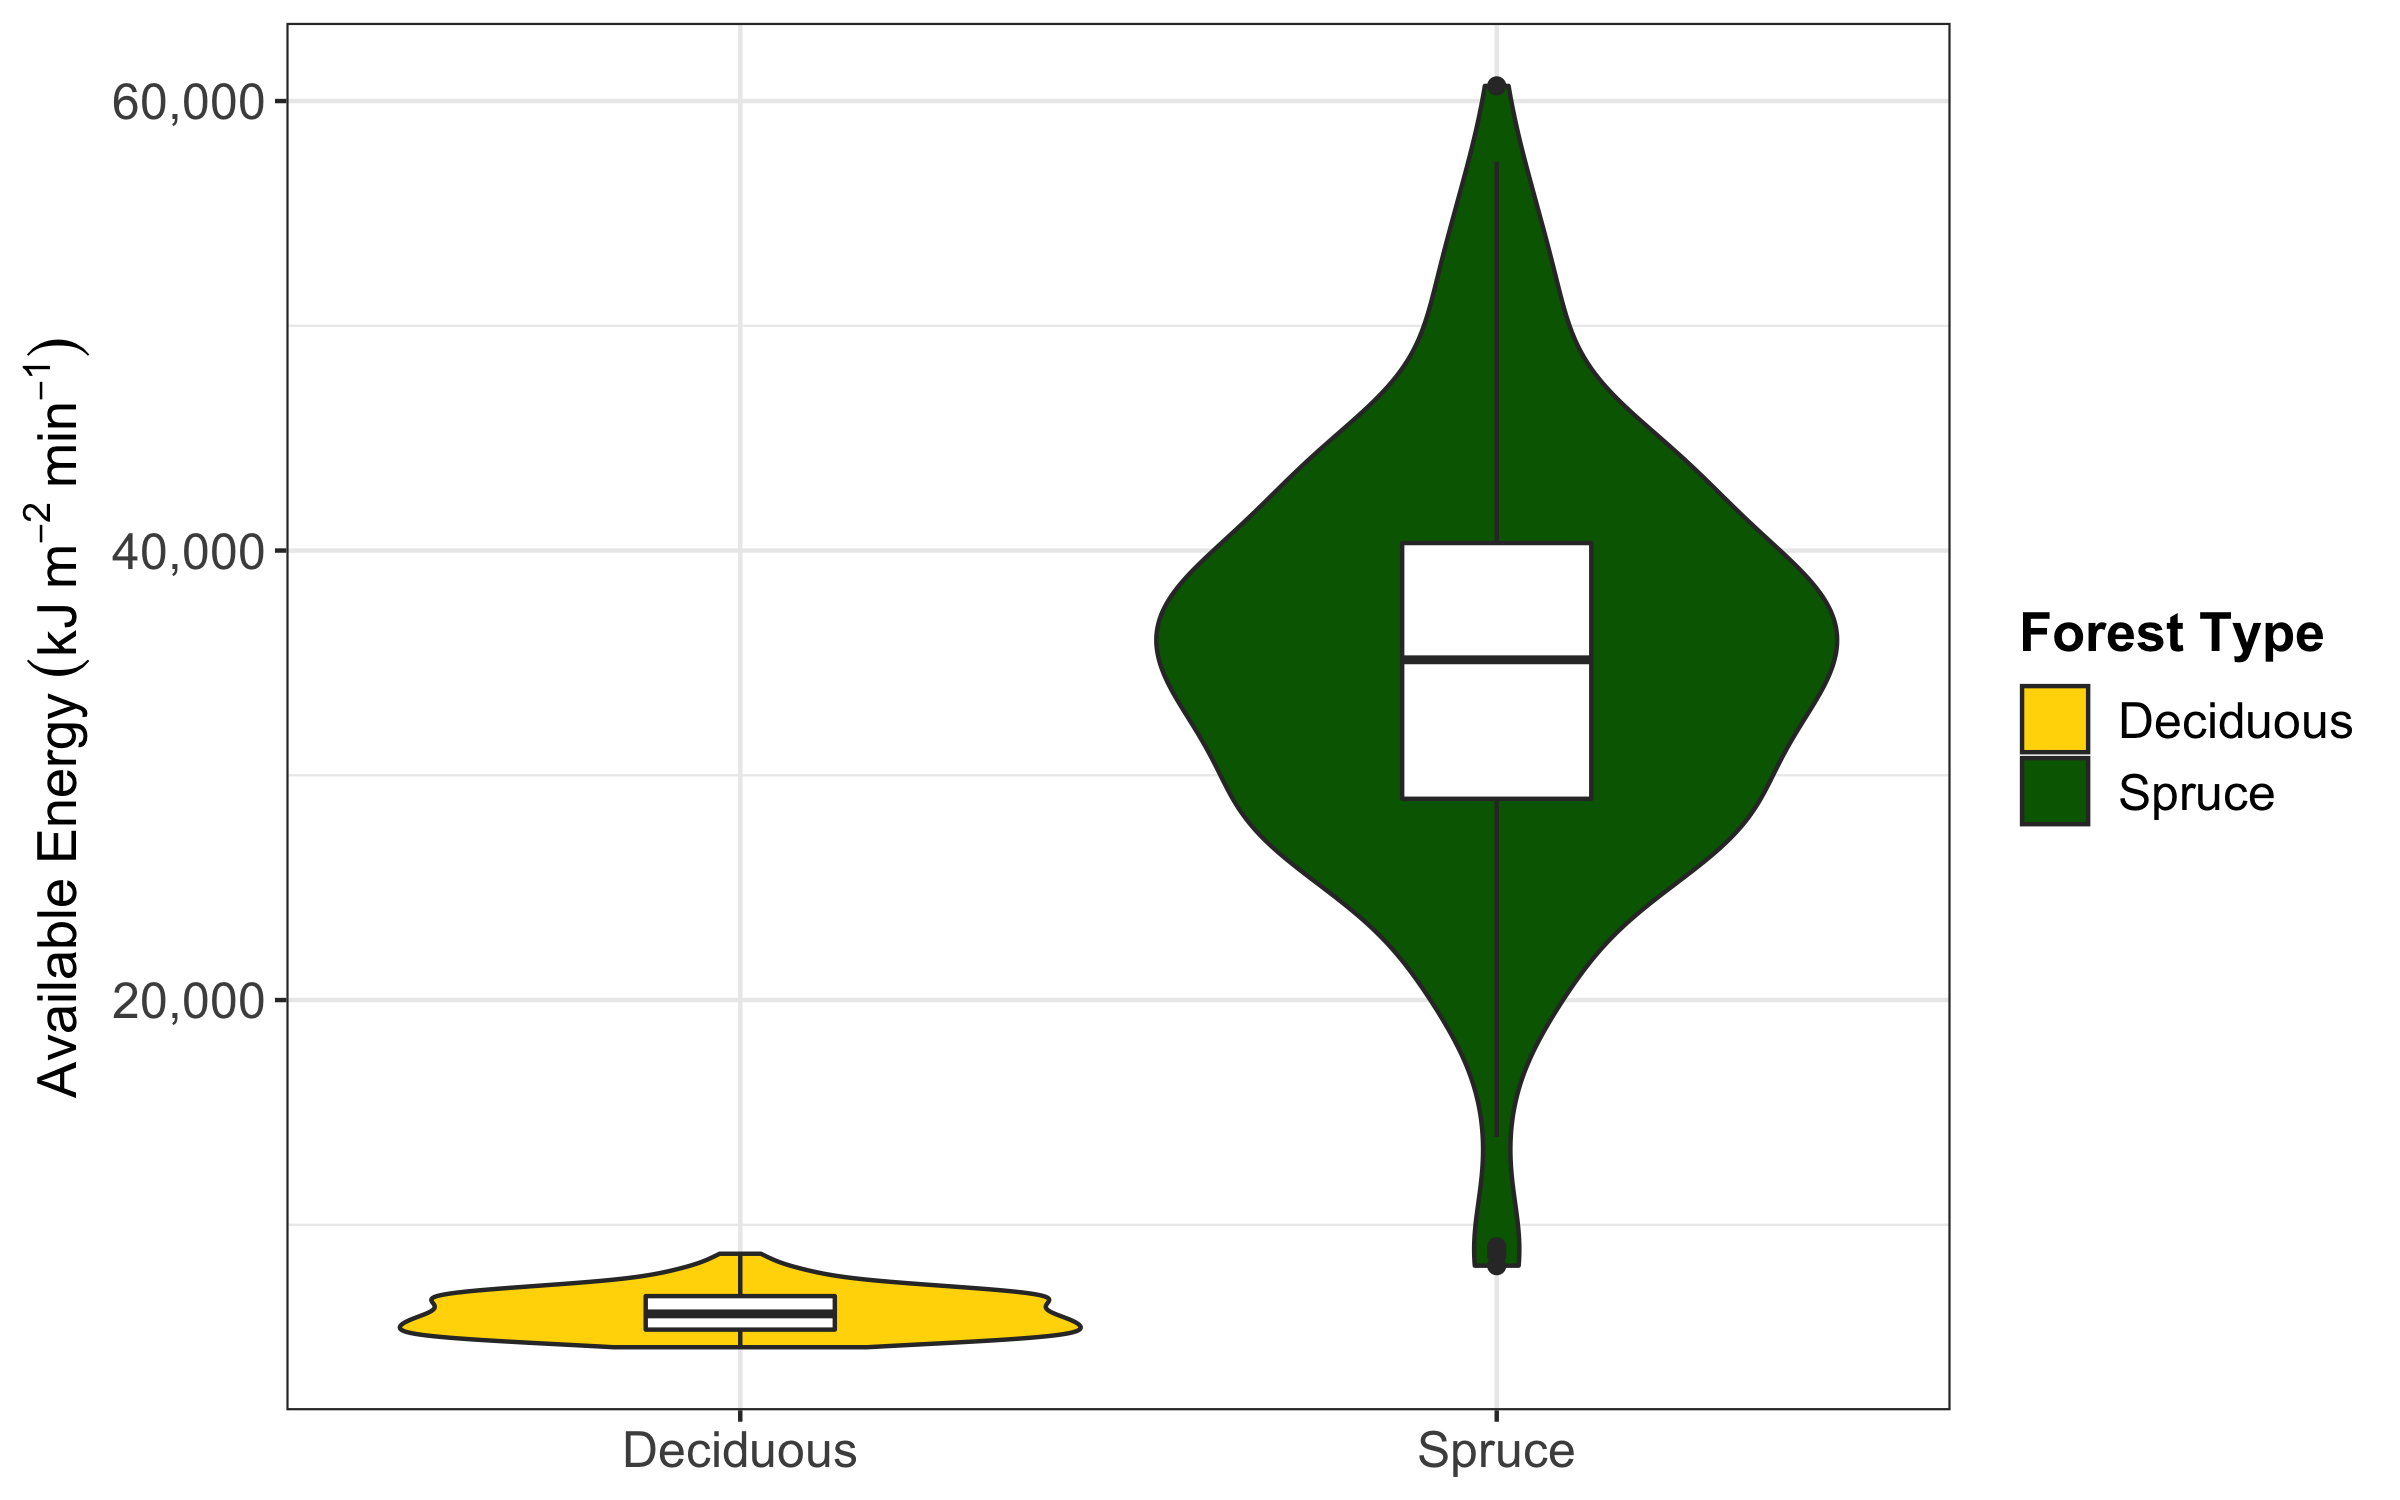
\includegraphics[width=\linewidth]{figures/avail_energy.png}
	\caption{Simulated available energy ($I_R\xi(1 + \theta)$, kJ m$^{-2}$ min$^{-1}$) for several hundred years at a black spruce site and a deciduous site. Due to the geometry and higher overall fuel loading, the spruce stand has much more energy available for combustion.}
	\label{fig:energy}
\end{figure}


The heat required for fuel ignition ($BD \cdot \epsilon \cdot Q_{ign}$) is calculated based on the fuel geometry and moisture. The effective heating number ($\epsilon$) determines the efficiency of fuel heating as a function of particle size \cite{rothermelMathematicalModelPredicting1972}:

\begin{equation}
	\epsilon = \text{e}^{\Big(\frac{-4.528}{\sigma}\Big)}
\end{equation}

A value of 1.0 would indicate 100\% of heating of zero-thickness fuel. The heat of preignition ($Q_{ign}$, kJ kg$^{-1}$) is based on fuel moisture:

\begin{equation}
	Q_{ign} = 581 + 2594m
\end{equation}

The ratio of available to required energy gives the rate of spread of a potential fire. As with available energy, ROS differs among different forest types (Fig. \ref{fig:rosf}).

\begin{figure}
	\includegraphics[width=\linewidth]{figures/rosf.png}
	\caption{Simulated rate of spread (m min$^{-1}$) for several hundred years at a black spruce site and a deciduous site.}
	\label{fig:rosf}
\end{figure}

\subsubsection{Fire Intensity} \label{fireintense}

Following potential rate of spread calculation, the surface fire intensity ($I_{surf}$, kW m$^{-1}$) is then calculated as in \citeA{thonickeInfluenceVegetationFire2010}:

\begin{equation}
	I_{surf} = h \cdot FC \cdot \frac{ROS}{60}
\end{equation}

where $FC$ is the fuel consumption (kg m$^{-2}$) from the fire. Fuel consumption for each litter type is calculated as:

\begin{equation}
	FC_i = w_{n_i}f_{b_i}
\end{equation}

where $w_{n_i}$ is the mineral fuel loading of each type (kg m$^{-2}$) and $f_{b_i}$ is the fraction burnt of each litter type, calculated as:

\begin{equation} \label{eq:fb}
	f_{b_i} = 
	\begin{cases}
		1.0, & \text{for } \frac{m}{m_x} \leq m_{min_i}  \\
		a_i\frac{m}{m_x}^2 + b_i\frac{m}{m_x} + c_i, & \text{for } m_{min_i}  < \frac{m}{m_x}  \leq 1 \\
		0.0, & \text{for } 1 < \frac{m}{m_x} 
	\end{cases}
\end{equation}

where $a_i$, $b_i$, and $c_i$ are litter type-specific parameters, and $m_{min_i}$ is the litter-specific threshold for relative moisture content. Individual fuel consumption values are summed to calculate the overall $FC$. Equation \ref{eq:fb} and parameters are modified from \citeA{thonickeInfluenceVegetationFire2010}.

\begin{figure}
	\includegraphics[width=\linewidth]{figures/frac_burnt.png}
	\caption{Relationship between relative fuel moisture and fraction burnt.}
\end{figure}

Fires with a surface intensity below 50 kW m$^{-1}$ cannot be sustained and are extinguished. Otherwise, the simulated fire burns plants, litter, and belowground material. Most fires in the North American boreal zone are high-intensity, stand-replacing fires \cite{rogersInfluenceTreeSpecies2015}, though they can vary between surface fires and very high-intensity crown fires \cite{vanwagnerFireBehaviorNorthern1983}. This updated fire model within UVAFME simulates this range of fire types based on fire intensity (Fig. \ref{fig:intensity}).

\begin{figure} 
	\includegraphics[width=\linewidth]{figures/Isurfhist.png}
	\caption{Distribution of UVAFME-simulated surface fire intensity (kW m$^{-1}$) for 300 sites across Canada and Alaska. Note the log-10 scale on the y-axis. Fire type categories are classified as in Van Wagner (1983).}
	\label{fig:intensity}
\end{figure}

\subsubsection{Crown Fires}

Many fires in the North American boreal zone become crown fires \cite{rogersInfluenceTreeSpecies2015},  either passive - when forest canopies burn but the fire does not spread through the canopy, or active - when the fire does spread through the canopy \cite{vanwagnerConditionsStartSpread1977}. 

We simulate crown fires in UVAFME using equations from \citeA{scottAssessingCrownFire2001} and \citeA{vanwagnerConditionsStartSpread1977}.  First, surface intensity must reach a critical level to allow passive crowning ($I_p$, kW m$^{-1}$), calculated as (Fig. \ref{fig:passivecrowning}):

\begin{equation}
	I_p = \Big(\frac{H_{cb}(460.0 + 25.9FMC)}{100.0}\Big)^{1.5}
\end{equation}

where $H_{cb}$ is the canopy base height (m), calculated as the minimum height in the canopy where canopy bulk density is greater than 0.011 kg m$^{-3}$, and $FMC$ is the foliar moisture content, set to a default of 100\%.  If the surface intensity is greater than this threshold value, crowning can occur.  If passive crowning is possible,  UVAFME then checks for an active crown fire.

\begin{figure} 
	\includegraphics[width=\linewidth]{Figures/passivecrowning.png}
	\caption{Relationship of canopy base height and the critical surface intensity for passive crowning in UVAFME - assuming foliar moisture content of 100\%.  With higher canopy base heights, a higher surface intensity is required for passive crown fires.}
	\label{fig:passivecrowning}
\end{figure}

For an active crown fire, the surface intensity needs to be high enough and the crown fuel needs to be dense enough to sustain the spread of a fire.  Critical rate of spread for an active crown fire ($ROS_a$, m s$^{-1}$) is calculated as (Fig. \ref{fig:activecrowning}):

\begin{equation}
	ROS_a = \frac{S_0}{\rho_c}
\end{equation}

where $S_0$ is the critical mass flow rate, default to 0.05 kg m$^{-2}$ s$^{-1}$, and $\rho_c$ is the canopy bulk density (kg m$^{-2}$). 

\begin{figure} 
	\includegraphics[width=\linewidth]{figures/activecrowning.png}
	\caption{Relationship of canopy bulk density and the critical rate of spread for active crowning in UVAFME. With lower canopy bulk densities, a higher ROS is required for active crown fires.}
	\label{fig:activecrowning}
\end{figure}

Actual active rate of spread is then calculated as:

\begin{equation} 
	ROS_{active} = 3.34\frac{I_R \cdot \xi \cdot (1 + \theta_w)}{BD \cdot \epsilon \cdot Q_{ign}}
\end{equation}

where the fuel characteristics (i.e.  loading and geometry) are based on fuel model (FM) 10,  as in \citeA{vanwagnerConditionsStartSpread1977}. 

Following \citeA{scottAssessingCrownFire2001}, the final rate of spread is calculated as 

\begin{equation}
	ROS_{final} = ROS_{surface} + CFB(R_{active} - R_{surface})
\end{equation}

where $CFB$ is the crown fraction burnt,  calculated as:


\begin{equation}
	CFM = \frac{ROS_{surface} - ROS_a}{R'_{SA} - ROS_a}
\end{equation}

where $R'_{SA}$ is the predicted surface fire spread rate that corresponds to the environmental conditions (i.e. wind speed) at which $R_{active} = R'_{active}$.  During an active crown fire, all crowns are assumed to burn at 100\%.

\subsubsection{Belowground Combustion}

In the North American boreal zone, combustion of belowground material is a highly important process. In contrast to aboveground flaming combustion, this belowground smoldering combustion occurs over longer time periods during and after the flaming front passage \cite{johnsonFireVegetationDynamics1992}. The total combustion and depth of burn depends on both organic layer moisture and the residence time of the fire \cite{johnsonFireVegetationDynamics1992, vanwagnerDuffConsumptionFire1972}.

Using an equation adapted from \citeA{vanwagnerDuffConsumptionFire1972}, we calculate combustion ($d$, kg m$^{-2}$) of the duff layer as (Fig. \ref{fig:duffcombust}):

\begin{equation}
	d = \frac{(60.0\tau_f)7.473\epsilon_f}{110.0 + 6.2(100.0m_{duff})}
\end{equation}

where $\epsilon_f$ is the emissivity of the fire (0-1), and $m_{duff}$ is the moisture content of duff (volumetric). $\tau_f$ is the residence time of the fire (min), calculated as \cite{petersonModelingPostfireConifer1986}:

\begin{equation} \label{eq:residence}
	\tau_f =  \sum_{i=1}^{9} \Big[3.94w_{n_i}\Big(1.0 - \sqrt{1.0 - f_{b_i}}\Big)\Big]
\end{equation}

where $f_{b_i}$ is the fraction burnt (0-1), $w_{n_i}$ is the mineral fuel loading (kg m$^{-2}$), and $i$ represents each fuel type, excluding boles and roots, and only including live canopy fuels (at $f_{b_i}$ = 1) under conditions of active crown fire.

\begin{figure} 
	\includegraphics[width=\linewidth]{figures/DuffCombust.png}
	\caption{Duff combustion relationship with duff moisture for two different fire residence times.}
	\label{fig:duffcombust}
\end{figure}

The fire emissivity ($\epsilon_f$) is calculated as \cite{vanwagnerDuffConsumptionFire1972}:

\begin{equation}
	\epsilon_f = 0.770 - 0.004(100.0m_{duff})
\end{equation}

and the duff moisture content is calculated using the duff moisture code (DMC):

\begin{equation}
	m_{duff} =20.0 + \text{exp}\Big(-1.0\frac{DMC - 244.72}{43.43})\Big) 
\end{equation}

Surface litter is combusted at the fraction ($f_b$) calculated in Section \ref{fireintense}. As in \citeA{fosterImportanceTreeSpecieslevel2019}, proportion nitrogen volatilization from combusted litter is calculated as:

\begin{equation}
	vol_N = 1.0 - \text{min}\Big(0.6426m_R + 3.34(z_{org} + z_{moss}), 0.7\Big)
\end{equation}

where $z_{org}$ and $z_{moss}$ are the depths (m) of the organic and moss layers, respectively, and $m_R$ is the relative moisture content, calculated as:

\begin{equation}
	m_R = \text{max}\Big(0.0, \frac{3.0 - m_{duff}}{3.0 - m_{pwp}}\Big)
\end{equation}

where $m_{pwp}$ is the permanent wilting point (volumetric) of the organic layer. Volatilized N is added to the plant-available N pool. 

\subsubsection{Fire Mortality, Live Fuel Combustion, and Post-Fire Regrowth}

As in \citeA{thonickeInfluenceVegetationFire2010} plant mortality from fire is considered based on both cambial damage and crown scorch. Damage from crown scorch is calculated based on scorch height ($SH$, m) of a fire \cite{petersonModelingPostfireConifer1986}.

\begin{equation}
	SH = F \cdot { I_{surf}}^{0.667}
\end{equation}

where $F$ is a species-specific parameter based on the lethal temperature for plant mortality. The value of $F$ depends on seasonality as well as whether buds or foliage are to be considered \cite{johnsonFireVegetationDynamics1992}. In this version, $F$ is set to a default of 0.11 for needle-leaved plants and 0.094 for broad-leaved plants \cite{thonickeInfluenceVegetationFire2010} (Fig \ref{fig:scorch}).

\begin{figure} 
	\includegraphics[width=0.75\linewidth]{figures/ScorchHeight.png}
	\caption{Scorch height relationship with surface fire intensity for broadleaf ($F$ = 0.095) and needleleaf ($F$ = 0.11) plants.}
	\label{fig:scorch}
\end{figure}

Assuming a cylindrical crown shape, the proportion of crown scorch ($CS$, 0 to 1) is calculated as:

\begin{equation}
	CS = \frac{SH - H + CL}{CL}
\end{equation}

where $H$ is the height of the plant (m) and $CL$ is the crown length of the plant (m). The probability of mortality from crown scorch is calculated as:

\begin{equation}
	p_{CS} = r(CS^p)
\end{equation}

where $r$ is the resistance factor for crown scorch survival, set to a default of 1.0, and $p$ is a parameter based on defoliation from crown scorch, set to a default of 3.0 \cite{thonickeInfluenceVegetationFire2010}.

Cambial damage is based on the residence time of the fire ($\tau_f$, Eq. \ref{eq:residence}) and the bark thickness of the plant. Probability of mortality from cambial damage is calculated as:

\begin{equation}
	p_{\tau} = 
	\begin{cases}
		0.0, & \text{for } \frac{\tau_f}{\tau_c} \leq 0.22  \\
		0.563\frac{\tau_f}{\tau_c} - 0.125, & \text{for } 0.22 \frac{\tau_f}{\tau_c}  \leq 2.0 \\
		1.0, & \text{for } 2.0 < \frac{\tau_f}{\tau_c} 
	\end{cases}
\end{equation}

where $\tau_c$ is a critical residence time (min) based on bark thickness:

\begin{equation}
	\tau_c = 2.8(DBH \cdot d_b)^2
\end{equation}

where $d_b$ is a bark thickness parameter (cm bark per cm DBH). Overall probability of mortality is calculated as:

\begin{equation}
	p_m = p_{\tau} + p_{CS} - p_{\tau}p_{CS}
\end{equation}


Within the proportion of crown scorched ($CS$), all of the 1-hr fuels are combusted (i.e. leaves and twigs), 50\% of the scorched small branches are combusted, 10\% of the scorched large branches are combusted, and 5\% of the scorched boles are combusted. Combustion occurs whether or not the individual dies by fire mortality. 

Non-combusted portions of plants that die from fire are added to the appropriate litter pools for decomposition (see \citeA{fosterImportanceTreeSpecieslevel2019}).

As in previous versions of UVAFME \cite{fosterImportanceTreeSpecieslevel2019, shumanFireDisturbanceClimate2017, fosterModelingInteractiveEffects2018}, immediately following a fire the seedbank ($s$, seeds m$^{-2}$) of each species is modified as $s = s\gamma$, where $\gamma$ ranges from 100.0 for fire-tolerant/serotinous species to 0.001 for fire-intolerant species.

The same year following a fire, no seedling establishment can occur. The subsequent years, seedling establishment is based on environmental conditions \cite{fosterImportanceTreeSpecieslevel2019} as well as organic and moss layer depth:

\begin{equation}
	f_{org} = 0.1 + \text{e}^{\Big(c(z_{org} + z_{moss})\Big)}
\end{equation}

where $c$ is a parameter ranging from -0.1 to -52.4 depending on species tolerance to regeneration on deep organic layers \cite{fosterImportanceTreeSpecieslevel2019}.

\subsection{Windthrow}

Windthrow disturbance is based on a site-specific input return intervals. Each plot run for a specific site has a probability windthrow ($p_{wind} = 1/WRI$) occurring each year. For each plot simulated and each year, a uniform random number between 0 and 1 is generated and if this value is below the wind probability ($p_{wind} = 1/WRI$) then a windthrow event occurs on the plot that year, independent from other plots or sites. The probability of windthrow mortality of each individual plant on the plot is based on plant size \shortcite{richWindthrowMortalitySouthern2007} (Fig \ref{fig:fpwind}):

\begin{equation}  \label{pwind}
p_{mwind} = \Big(1.0 + \text{e}^{-0.75\ln(D)}\Big)^{-1}
\end{equation}

\begin{figure}
  \includegraphics[width=0.65\linewidth]{Figures/pwind.png}
  \caption{Probability of windthrow mortality with increasing diameter (Eq. \ref{pwind}) \protect\cite{richWindthrowMortalitySouthern2007}.}
  \label{fig:fpwind}
\end{figure}

The components of plants that die by windthrow are added to the appropriate litter cohorts as with mortality from age- or growth-related stress. If the individual does not die, annual litterfall is calculated as above (Eq. \ref{annlit}).

\subsection{Insects}
UVAFME is also able to simulate mortality from the spruce beetle (\textit{Dendroctonus rufipennis} (Kirby)), a bark beetle which infests spruce (\textit{Picea} spp.) species. Mortality is simulated as the probability of infestation of each host tree based on climate-, site-, and plant-level characteristics \cite{fosterModelingInteractiveEffects2018}. 

Climate factors for this submodel were derived from studies on the phenology of spruce beetles and what influences their shift from a semivoltine to a univoltine life cycle \shortcite{hansenTemperaturebasedModelPredicting2001, sherriffClimateVariabilitySpruce2011, hansenPrepupalDiapauseInstar2011}. Based on a detailed spruce beetle phenology study by \citeA{hansenTemperaturebasedModelPredicting2001}, calculations were included to determine whether the beetle population on each plot has a semivoltine (two-year) or univoltine (one-year) life cycle. This calculation is based on the cumulative hours above 17ºC during the period of 40 to 90 days prior to the beetles’ peak flight. Cumulative hours above 17ºC during this period are calculated using a sinusoidal temperature formula from \citeA{reicoskyAccuracyHoulyAir1989} (Section \ref{climate}; Eq. \ref{hourlytemp}). This equation is then used to accumulate the number of hours above 17ºC ($H_{17}$) during 40 to 90 days prior to peak spruce beetle flight. Cumulative hours above 17ºC is equal across all plots within an individual site, but may change from year to year and from site to site. The probability of any one plot having beetles with a univoltine life cycle ($p_{uv}$; Eq. \ref{puv}; Fig \ref{fig:fpuv}), from \citeA{hansenTemperaturebasedModelPredicting2001}, is then calculated and is used to influence the infestation probability of each individual tree on that plot.

\begin{equation} \label{puv}
p_{uv} = \Big(1.0 + \text{e}^{3.954 - 0.01944H_{17}}\Big)^{-1}
\end{equation}

\begin{figure}
  \includegraphics[width=0.65\linewidth]{Figures/puv.png}
  \caption{Probability of univoltine (one year life cycle) beetle populations with cumulative hours above 17ºC during the period between 40 and 90 days prior to peak beetle flight (Eq. \ref{puv}) \protect\cite{hansenTemperaturebasedModelPredicting2001}.}
  \label{fig:fpuv}
\end{figure}

Plot-level factors are calculated each year based on individual plot characteristics, and thus will vary between the simulated plots at a given site. These plot-level factors are based on spruce beetle susceptibility stand ratings from \citeA{schmidStandRatingsSpruce1976}. As in their stand rating system, this model uses average DBH of live spruce above 25.4 cm DBH, plot-level spruce basal area, and percent of spruce in the canopy as factors for determining plot-wide susceptibility to spruce beetle attacks. Depending on the value of each of the three factors, each plot receives three factor ratings from 1 to 3 (Table \ref{tab:sbratings}), and the ratings from each individual factor are added together to produce an overall stand rating (possible values being 3 to 9). 

\begin{table}
  \begin{center}
    \caption{Values of plot factors associated with each factor rating used to calculate overall plot-wide susceptibility to spruce beetle infestation from \protect\citeA{schmidStandRatingsSpruce1976}.}
    \label{tab:sbratings}
\resizebox{\linewidth}{!}{%
\begin{tabular}{c|c|c|c|l}
\cline{2-4}
& \multicolumn{3}{c|}{\textbf{Plot Factor Value}} \\ \cline{1-4}
\multicolumn{1} {|c} {\begin{tabular}{c}\textbf{Susceptibility} \\ \textbf{Rating} \end{tabular}} & 
\multicolumn{1} {|c|}{\begin{tabular}{c} Basal area of \\ spruce in the \\stand (m$^2$ ha$^{-1}$)\end{tabular}} & 
\begin{tabular}{c} Mean DBH \\of live spruce \\ over 24.5 cm DBH (cm) \end{tabular} & 
\begin{tabular}{c} Percent spruce \\ in canopy (\%) \end{tabular} & \\ \cline{1-4}
\multicolumn{1}{ |c| }{Low (1)} & $<$ 22.95 & $<$ 30.48 & $<$ 50 & \\ \cline{1-4}
\multicolumn{1}{ |c| }{Medium (2)} & 22.95 to 34.43 & 30.48 to 40.64 & 50 to 65 & \\ \cline{1-4}
\multicolumn{1}{ |c| }{High (3)} & $\geq$34.43 & $\geq$40.64 & $\geq$65 & \\ \cline{1-4}
\end{tabular}}
  \end{center}
\end{table}

The overall stand rating is then used to calculate the probability for spruce beetle infestation in each tree due solely to plot characteristics ($f_{stand}$, 0 to 1; Eq. \ref{fstand}; Fig. \ref{fig:ffstand}). This stand-level probability is utilized to calculate the individual-tree infestation probability (Eq. \ref{ftree}) and is the same for every tree on the same plot in a given year.

\begin{equation} \label{fstand}
f_{stand} = 0.75\ln(f_{BA} + f_{DBH} + f_{can}) - 0.8
\end{equation}

\begin{figure}
  \includegraphics[width=0.65\linewidth]{Figures/fstand.png}
  \caption{Stand susceptibility with increasing stand ratings from Table 2.4. Stand ratings are derived from \protect\citeA{schmidStandRatingsSpruce1976}.}
  \label{fig:ffstand}
\end{figure}

where $f_{BA}$ is the factor rating from column one, $f_{DBH}$ is the factor rating from column two, and $f_{can}$ is the factor rating from column three of Table \ref{tab:sbratings}. This overall stand rating is then modified based on recent windthrow events to account for the high influence of blowdown on bark beetle outbreaks \shortcite{christiansenResistanceConifersBark1987, wichmannSpreadIpsTypographus2001, mezeiHostSiteFactors2014}. Following a windthrow event, the overall stand infestation probability is increased by 0.3 for the first three years, 0.2 from four to six years, and 0.1 from five to nine years. Because spruce beetle populations can utilize downed spruce trees (from windthrow or other mortality factors) for reproduction at low levels \cite{schmidSpruceBeetleRockies1977}, plot-wide susceptibility is also influenced based on the amount of coarse woody debris on the plot available for spruce beetle colonization. Spruce trees larger than 25.4 cm DBH that die from either windthrow, age, or low growth are added to a pool of coarse woody debris ($CWD_{spruce}$, tonnes C ha$^{-1}$). A plot-wide woody debris factor ($f_{cwd}$, 0 to 1) is then calculated, which increases linearly with increasing spruce woody debris:

\begin{equation} \label{fcwd}
f_{cwd} = \min\Big(\frac{CWD_{spruce}}{CWD_{base}}, 1.0\Big)
\end{equation}

where $CWD_{base}$ is set to 300 tonnes C ha$^{-1}$, corresponding to potential coarse woody debris that may occur from a very severe windthrow event, as in \shortciteA{temperliCrossscaleInteractionsBark2013}. Spruce coarse woody debris decays as with other large boles (Section \ref{nutrients}).

Tree-level factors that affect the probability of spruce beetle infestation include individual tree size ($f_{tDBH}$), stress level ($f_{stress}$), and scorch volume from recent fires ($f_{scorch}$). Under normal conditions, trees that are smaller than 30 cm DBH are not susceptible to spruce beetle attack \cite{deroseDroughtdrivenDisturbanceHistory2012}. Under epidemic conditions (i.e. greater than 10 m$^2$ ha$^{-1}$ of basal area killed per year) trees as small as 10 cm DBH may be killed by spruce beetles \cite{peetForestVegetationColorado1981, veblenDisturbanceRegimeDisturbance1994, deroseDroughtdrivenDisturbanceHistory2012}. Otherwise, based on information from relevant literature on bark beetle infestations \shortcite{furnissChronologyCharacteristicsDouglasfir1979, negronProbabilityInfestationExtent1998, hoodPredictingPostfireDouglasfir2007, zolubasModellingSpruceBark2009, mezeiHostSiteFactors2014} and inventory data from the US Forest Service, infestation probability due to tree size ($f_{tDBH}$, 0 to 1) increases linearly with increasing tree diameter (Eq. \ref{ftdbh}). 

\begin{equation} \label{ftdbh}
f_{tDBH} = \min(0.011DBH, 1.0)
\end{equation}

Many studies have shown that prolonged stress and associated low tree vigor, due to drought, age, or other factors, increases a tree’s susceptibility to bark beetle attacks \shortcite{kalksteinEffectsClimaticStress1976, waringSimpleModelHost1980, larssonAttacksMountainPine1983, christiansenResistanceConifersBark1987, mattsonRoleDroughtOutbreaks1987, malmstromBioticDisturbanceAgents2000, mckenzieChapter15Global2009}. In this model, tree stress is quantified as prolonged low diameter increment growth (i.e. less than 0.03 cm per year). Probability of spruce beetle infestation due to stress level ($f_{stress}$, 0 to 1) increases by 0.1 each year the tree in question has diameter growth below 0.03 cm, and is reset to 0 if the tree has higher than 0.03 cm growth in any given year. Damage due to fire has also been cited as a potential precursor to bark beetle attack \shortcite{geiszlerBarkBeetleInfestations1984, christiansenResistanceConifersBark1987, rasmussenBarkBeetleWood1996, hoodPredictingPostfireDouglasfir2007}. UVAFME calculates fire damage by percent crown volume scorched ($CS$, \%) based on fire dynamics equations from \citeA{keaneFireBGCv2LandscapeFire2011} and \citeA{schumacherModelingImpactClimate2006} (see above Fire section). In this spruce beetle model, susceptibility to beetle infestation based on fire damage ($f_{scorch}$, 0 to 1) is equal to the proportion of crown volume scorched by wildfire. 

As with the individual plot-level factors, these tree-level factors are combined, along with the overall plot-wide factors, to produce an overall tree-level susceptibility to spruce beetles ($f_{tree}$, 0 to 1; Eq. \ref{ftree}). 

\begin{equation} \label{ftree}
f_{tree} = \min\Big(0.3f_{stand} + 0.25f_{tDBH} + 0.2f_{stress} + 0.1f_{scorch} + 0.4f_{cwd}, 1.0\Big)
\end{equation}

Coefficients associated with each susceptibility factor are based on susceptibility ratings from relevant literature \shortcite{schmidStandRatingsSpruce1976, seidlModellingTreeMortality2007, hartTreeStandlevelAttributes2014}. This susceptibility is used to calculate the final tree-level probability for spruce beetle infestation (Eq. \ref{bprob}, Fig. \ref{fig:bbprob}):

\begin{equation} \label{bprob}
p_{beetle} = 1.0 - {\text{e}^{(-2.0{f_{tree}}^{1.3})}}^{gen}
\end{equation}

where $gen$ is equal to 1.8 if the plot in question has univoltine beetles (based on uniform random number draws compared to the probability for univoltinism - $p_{uv}$; Eq. \ref{puv}) and 0.5 if it does not. Equation \ref{bprob} was adapted from a bark beetle modeling study by \citeA{seidlModellingTreeMortality2007} on the European spruce bark beetle in Norway spruce forests.

\begin{figure}
  \includegraphics[width=0.8\linewidth]{Figures/pbeetle.png}
  \caption{Probability of beetle infestation increases with increasing tree susceptibility ($f_{tree}$, Eq. \ref{ftree}) and with univoltine beetle populations (Eq. \ref{bprob}).}
  \label{fig:bbprob}
\end{figure}

Once a tree becomes infested by spruce beetles, it ceases growth (i.e. $\delta DBH_{actual} = 0.0$ - see Section {\ref{tgrowth}}) \shortcite{frankEcosystemCOFluxes2014}, and loses its needles after two years (i.e. $LA = 0.0$ - see Section \ref{allometry}) \cite{schmidSpruceBeetleRockies1977}. Finally, after five years of being infested, the tree is set to fall and its component parts are added to the appropriate litter cohorts for decomposition (Section \ref{nutrients}). A study by \shortciteA{hartTreeStandlevelAttributes2014} found that proximity to infested spruce trees was an important factor in determining infestation probability. Thus, within this spruce beetle submodel, during the time when a tree is infested and still on a plot it increases the infestation probability of directly (by 0.3) and diagonally (by 0.1) adjacent spruce trees on the same plot (see Section \ref{treeregen} for more on tree positions). 

\section{Regeneration} \label{regen}
\numberwithin{equation}{section}

Annual establishment of new trees and shrubs in UVAFME is based on the species-specific seed and seedling banks on each plot as well as the current environmental conditions and species-specific tolerances. Similar to other gap models, the species of each new plant established is determined stochastically, weighted by each species' ability to survive in the current plot's environment. The seedbank and seedling bank of each species is additionally modified to account for seeding strategies (i.e. serotiny, sprouting etc.) and natural mortality of seeds and seedlings \cite{yanFAREASTForestGap2005}.

New plants are only established if the available N ($N_{avail}$) is still above 0 tonnes N ha$^{-1}$ from N use in annual plant growth (Section \ref{tgrowth}). If there is any available N, a species-specific regrowth variable ($r_{new_{sp}}$, 0 to 1) is calculated based on the current environmental conditions and species-specific tolerances:

\begin{equation} \label{rnew}
r_{new_{sp}} =  f_{perm}f_{gdd}f_{drought}f_{light}f_{N}
\end{equation}

This regrowth variable is additionally modified to account for the amount of reproductively mature plants on the plot. For each species, if any plants of that species are older than the minimum age for reproduction (default of 10 years for most species) then $r_{new_{sp}}$ is not modified. Otherwise, $r_{new_{sp}}$ is multiplied by 0.50 as in \citeA{bonanComputerModelSolar1989}. Finally, if $r_{new_{sp}}$ is at or below the minimum growth threshold ($\delta DBH_{min}$) then it is set to 0.0, otherwise no change is applied. The maximum regrowth variable ($r_{new_{max}}$, 0 to 1) is set as the maximum value of $r_{new_{sp}}$ across all species.

These values are used to calculate total number of plants to renew this year:

\begin{equation} 
nr_{max} = \min\Big(nt_{max}r_{new_{max}} - nt, nt_{max}\Big)
\end{equation}

and

\begin{equation}  \label{newtrees}
nr = \min\Big(\max(nr_{max}, 3), nt_{max} - nt\Big)
\end{equation}

where $nr_{max}$ is the maximum amount of renewable plants, $nt$ is the current number of plants on the plot, $nt_{max}$ is the maximum number of plants allowed on a plot and $nr$ is the number of plants to be renewed this year.

\subsection{Seed and Seedling Banks} \label{seeds}

The species of each plant to be established is determined using annual modifications to species-specific seed and seedling banks. The seedbank for each species (seeds m$^{-2}$) is updated as:

\begin{equation} \label{Sbank}
S_{bank} = S_{bank} + inv + s_{num}sp_{avail}
\end{equation}

where $inv$ is a species-specific input parameter indicating the number of seeds from outside the plot (seeds m$^{-2}$), with wind dispersed seeds generally have an $inv$ value of 1.0; $s_{num}$ is a species-specific input parameter indicating the number of seeds that could be produced from within the plot (seeds m$^{-2}$); and $sp_{avail}$ is a variable indicating the presence and reproduction ability of each species on the plot (Eq. \ref{avspec}).

\begin{equation} \label{avspec}
sp_{avail} = \begin{cases}
1.0, & \text{if any $D_{t_{sp}} - D_{max_{sp}}\delta D_{min} > 0.0$} \\
0.0, & \text{otherwise}
\end{cases}
\end{equation}

where $D_{t_{sp}}$ is the diameter of any tree (DBH) or shrub (basal diameter) of species $sp$ and $D_{max_{sp}}$ is the average maximum diameter of species $sp$. The seedbank is additionally modified to incorporate the effects of fire (if fire occurred that year):

\begin{equation} 
S_{bank} = S_{bank}k_{fire}
\end{equation}

where $k_{fire}$ is a parameter ranging from 0.001 to 1000, depending on the input species-specific regeneration tolerance to fire - ranging from 1 (fire is very beneficial to regeneration) to 5 (fire is very detrimental to regeneration).

If the species-specific regrowth variable calculated above ($r_{new_{sp}}$, Eq. \ref{rnew}) is greater than $\delta DBH_{min}$, then all seeds in the seed bank are moved to the species' seedling bank and the seedbank is set to 0.0. Otherwise, no seeds are added to the seedling bank and the seedbank is multiplied by the species-specific parameter $NDS$, which represents the annual percentage loss of seeds for each species. 

As in \citeA{bonanCarbonNitrogenCycling1990} and \citeA{bonanSimulationMossTree1989}, if seeds are added to the seedling bank, it is then modified by a variable related to the depths of the organic and moss layers, $d_{org}$ and $d_{moss}$ (m, Sections \ref{nutrients} and \ref{moss}):

\begin{equation} \label{forg}
f_{org} = \begin{cases}
\text{e}^{-7.4(d_{org} + d_{moss})}, & \text{$tol_{org} = 1$} \\
\text{e}^{-52.4(d_{org} + d_{moss})}, & \text{$tol_{org} = 2$} \\
\end{cases}
\end{equation}

where $tol_{org}$ is a species-specific organic/moss layer depth tolerance parameter (1: tolerant; 2: intolerant). This value is multiplied by the seedling bank number ($SL_{bank}$). The above equation was modified from \citeA{bonanSimulationMossTree1989} using data on post-fire seedling counts from \shortciteA{johnstoneChangesFireRegime2010}.  The seedling bank is then additionally modified to account for layering and sprouting. If the combined depths of the organic and moss layers is greater than 5 cm, and the species is able to reproduce by layering, the species' seedling bank is multiplied by 1.8 as in  \citeA{bonanComputerModelSolar1989}. 

If the species is able to produce sprouts, the species' seedling bank is updated as: $SL_{bank} = SL_{bank} + n_{sprouts}sp_{avail}$, where $n_{sprouts}$ is a species-specific input parameter indicating how many sprouts per plant the species can produce.

\subsection{Establishment} \label{treeregen}

New trees and shrubs are generated using the total number of plants to be established ($nr$, Eq. \ref{newtrees}), as well as the size of each species' seedling bank and each species' regrowth variable ($r_{new_{sp}}$, Eq. \ref{rnew}). Each species' seedling bank is converted from seedlings m$^{-2}$ to seedlings plot$^{-1}$ and used to calculate a species-specific establishment variable, $e_{sp}$ (seedlings plot$^{-1}$):

\begin{equation} 
e_{sp} = SL_{bank}r_{new_{sp}}
\end{equation}

Each individual $e_{sp}$ value is summed across all species to calculate an overall $e_{sum}$ value. Each species' $e_{sp}$ value is converted to a relative/probability of establishment parameter: $e_{r} = e_{sp}/e_{sum}$ (0 to 1), and then to a cumulative probability parameter ($e_{c}$, 0 to 1). 

Subsequently, $nr$ plants are renewed, and for each plant the species is determined by random uniform draws compared to the cumulative establishment probability. Once a species is determined, the seedling bank for that species is decreased by one. 

Plants in UVAFME are located on a grid (generally 30$\times$30). Currently, plants within the same plot interact spatially with one another with respect to insect infestation (Section \ref{disturbances}). When a new plant is established, its x/y location on the grid is drawn randomly from the set of empty grid spaces on the plot. The plant then carries this same grid cell location throughout its lifetime until its death, at which point that grid cell is once again empty.

New trees and shrubs that are established are assigned a random diameter via: $D = 1.5 + r$ for trees and $D = 0.3 + r$ for shrubs, where $r$ is a normally distributed random number (mean = 0.0; sd = 1.0). The new plant's diameter is restricted to be values between 0.5 and 2.5 cm for trees and 0.1 and 0.5 for shrubs. Tree clear branch bole height ($H_{cbb}$, m) is set to 1.0 m, and all other plant allometric characteristics (height, diameter at clear branch bole height, and biomass) are calculated using equations from Section \ref{allometry}.

Annual litter from newly established plants is calculated as with equation \ref{annlit}. After all new plants have been established and decremented from the relevant species' seedling bank, each species seedling bank is updated and converted back to seedlings m$^{-2}$ as:

\begin{equation} 
SL_{bank} = \frac{SL_{bank}NDE}{plotsize}
\end{equation}

where $NDE$ is a species-specific input parameter representing the percentage annual loss of seedlings. 

\section{Random Processes} \label{random}
\numberwithin{equation}{section}

Stochasticity is incorporated throughout UVAFME in the climate, (Section \ref{climate}), mortality (Section \ref{mortality}), and regeneration (Section \ref{regen}) subroutines via pseudorandom number generators.

\subsection{Random Number Seeds}

Random number generator seeds are used in the pseudorandom number generators. In this version, the seed can be fixed across all sites run ($fixed\_seed = \text{TRUE}$) or it can be different for each site. If the seed is fixed, the seed is reset for each site. Using the same seed ensures reproducibility (i.e. the same random numbers are generated each time the same site is run). 

If $fixed\_seed = \text{TRUE}$, the default seed or a user-supplied seed is used at the beginning of each site's run to set up the number generators. If $fixed\_seed = \text{FALSE}$ and no seed is supplied, new seeds are used for each site. In this case, the Fortran intrinsic function \textbf{date\_and\_time} is used to get the milliseconds of the current second ($idate$). The Fortran intrinsic \textbf{random\_seed} is then used to get a random seed ($iseed$). This value is then modified as:

\begin{equation} 
iseed = \begin{cases}
iseed \times idate, & \text{$iseed \neq 0$} \\
default\_seed \times idate, & \text{$iseed = 0$}
\end{cases}
\end{equation}

where $default\_seed$ is a default integer seed (size 7) within the model. This seed is set as the random number seed for subsequent random number calls.

\subsection{Pseudorandom Number Generators}

Four different pseudorandom number generators are used in the model: a uniform random number generator, a normally distributed random number generator, and two climate variable-specific uniform and normally distributed random number generators. The climate variable-specific generators are only used in creating the monthly and daily values of temperature, precipitation, and cloud cover from their input distributions. The other two generators are used for all other random number calls.

\subsubsection{Uniform Random Numbers}

The climate-specific uniform random number generator is created using a linear congruent method with a shuffle \shortcite{pressNumericalRecipesPascal1989}. The regular uniform random number generator (i.e. for all uniform random calls \textit{except} climate variables) uses the Fortran intrinsic function \textbf{random\_number} to generate a uniform random number. This generator uses two separate congruential generators and produces a period of $~10^{18}$ \shortcite{lecuyerEfficientPortableCombined1988, bratleyGuideSimulation1987}.

For both generators, the uniform random number is then modified as:

\begin{equation} 
urand = lb + (ub - lb)urand
\end{equation}

where $lb$ and $ub$ are lower and upper bounds for the number, respectively, default to $lb = 0.0$ and $ub = 1.0$. Both generators show pseudorandom results with a uniform distribution [0, 1) (Fig. \ref{fig:urand}).

\begin{figure}
  \includegraphics[width=0.8\linewidth]{Figures/Urand.png}
  \caption{Example simulation of uniform random numbers using the regular and climate-specific pseudorandom number generators (n = 2333100, mean$_{clim} \approx$ 0.5004, mean$_{reg} \approx$ 0.5002, sd$_{clim} \approx$ 0.2884, sd$_{reg} \approx$ 0.2887; $\sigma$ of a uniform distribution = $\sqrt{\frac{(lb - ub)^2}{12}}, \approx 0.2887$ when $lb = 0.0$ and $ub = 1.0$).}
  \label{fig:urand}
\end{figure}

\subsubsection{Random Normals}
The climate-specific normally distributed random number generator uses the climate-specific uniform random number generator and the Box-Muller polar method to generate a normally distributed random number with a specified mean and standard deviation (default to mean = 0.0, sd = 1.0). Two random uniforms are generated between -1 and 1 and these values are used to calculate:

\begin{equation} 
w = \sqrt{\frac{-2.0\ln({urand_1}^2 + {urand_2}^2)}{{urand_1}^2 + {urand_2}^2}}
\end{equation}

where ${urand_1}^2 + {urand_2}^2$ must not equal 0.0 or be greater than 1.0. The random normal is then calculated as:

\begin{equation} 
nrand = (urand_1w)sd + mn
\end{equation}

where $mn$ and $sd$ are the input/default mean and standard deviation. The regular normally distributed random number generator also uses the Box-Muller polar method, but with the regular uniform random number generator to generate the initial two random uniforms. Both generators show pseudorandom results with a normal distribution (mean = $mn$, standard deviation = $sd$) (Fig \ref{fig:nrand}).

\begin{figure}
  \includegraphics[width=0.8\linewidth]{Figures/Nrand.png}
  \caption{Example simulation of normally distributed random numbers using the regular and climate-specific pseudorandom number generators (n = 2333100, mean$_{clim} \approx$ -0.0042, mean$_{reg} \approx$ -0.00044, sd$_{clim} \approx$ 1.002, sd$_{reg} \approx$ 1.0002).}
  \label{fig:nrand}
\end{figure}

\bibliographystyle{apacite} 
 \bibliography{ReferencesNew}
 
\end{document}